\documentclass[letterpaper,12pt,oneside]{book}
\usepackage{blindtext}
\usepackage[utf8]{inputenc}
\usepackage[T1]{fontenc}
\setlength{\emergencystretch}{3em} % Evita líneas desbordadas.
\usepackage[spanish,es-noshorthands,es-tabla]{babel}
\usepackage{amsmath}
\DeclareMathOperator{\mcd}{mcd} % Máximo Común Divisor (versión en español de \gcd)
\DeclareMathOperator{\sen}{sen} % Seno en español.
\usepackage{amsfonts}
\usepackage{amssymb}
\usepackage{graphicx}
\usepackage{tabularx}
\graphicspath{{../assets/images/}{thesis/assets/images/}{Shack_Hartman_Con_corrimiento_de_puntos/thesis/assets/images/}}
\usepackage{wrapfig}
\usepackage{float}
% Parámetros de flotantes: evitan hojas de solo figura con grandes blancos.
\renewcommand{\topfraction}{.9}\renewcommand{\bottomfraction}{.8}\renewcommand{\textfraction}{.1}\renewcommand{\floatpagefraction}{.8}
\usepackage[font={small,it},labelfont={bf,up}]{caption}
% Títulos de sección y subsección alineados a la izquierda.
\makeatletter
\renewcommand\section{\@startsection{section}{1}{\z@}{-3.5ex \@plus -1ex \@minus -.2ex}{2.3ex \@plus.2ex}{\normalfont\Large\bfseries\raggedright}}
\renewcommand\subsection{\@startsection{subsection}{2}{\z@}{-3.25ex\@plus -1ex \@minus -.2ex}{1.5ex \@plus .2ex}{\normalfont\large\bfseries\raggedright}}
\makeatother
\usepackage{listings}
\usepackage{latexsym}
\usepackage[hidelinks]{hyperref}
\usepackage[absolute,overlay]{textpos}
\lstset{
	basicstyle=\footnotesize\ttfamily,  % Estilo básico del texto del código
	numbers=left,                       % Posición de los números de línea
	numberstyle=\tiny,                  % Estilo de los números de línea
	frame=single,                       % Añade un marco alrededor del código
	breaklines=true,                    % Permite romper líneas
	postbreak=\mbox{\textcolor{red}{$\hookrightarrow$}\space},  % Indicador de salto de línea
	keywordstyle=\color{blue},          % Estilo de las palabras clave
	commentstyle=\color{gray}           % Estilo de los comentarios
}

\author{Carlos Enrique Valderrama Juárez}
\title{Shack-Hartmann con corrimiento de puntos}




\begin{document}

	\begin{titlepage}
		\thispagestyle{empty}
		% Los elementos administrativos privados se cargan solo cuando están disponibles.
		\IfFileExists{private/frontmatter-approval.tex}{%
			\input{private/frontmatter-approval.tex}%
		}{}
		\begin{minipage}[c][0.17\textheight][c]{0.25\textwidth}
			\begin{center}


			\end{center}
		\end{minipage}
		\begin{minipage}[c][0.195\textheight][t]{0.75\textwidth}
			\begin{center}
				\vspace{0.3cm}
				\textsc{\large \textbf{UNIVERSIDAD NACIONAL AUTÓNOMA DE MÉXICO} \\	ciudad universitaria}\\[0.5cm]
				\vspace{0.3cm}
				\hrule height2.5pt
				\vspace{.2cm}
				\hrule height1pt
				\vspace{.8cm}
				\textsc{Maestría en ingeniería eléctrica - instrumentación óptica\\}
				\vspace{1.5cm} %
			\end{center}
		\end{minipage}
	
	 \begin{minipage}[c][0.81\textheight][t]{0.25\textwidth} 
		\vspace*{5mm}
		\begin{center}
			\hskip2.0mm
			\vrule width1pt height13cm 
			\vspace{5mm}
			\hskip2pt
			\vrule width2.5pt height13cm
			\hskip2mm
			\vrule width1pt height13cm \\
			\vspace{5mm}
			
		\end{center}
	\end{minipage}
\begin{minipage}[c][0.81\textheight][t]{0.75\textwidth}
	\begin{center}
		\vspace{1cm}
		
		{\large\scshape  \textbf{SHACK-HARTMANN CON CORRIMIENTO DE PUNTOS}}\\[.2in]
		
		\vspace{2cm}            
		
		\textsc{\LARGE T\hspace{1.5cm}E\hspace{1.5cm}S\hspace{1.5cm}I\hspace{1.5cm}S}\\[0.5cm]
		\textsc{\large que para obtener el t\'itulo de:}\\[0.5cm]
		\textsc{\large Maestro en ingeniería}\\[0.5cm]
		\textsc{\large presenta:}\\[0.5cm]
		\textsc{\large {Carlos Enrique Valderrama Juárez}}\\[2cm]          
		
		\vspace{0.5cm}
		
		{\large\scshape Tutor:\\[0.3cm] {Dr. José Rufino Díaz Uribe}}\\[.2in]
		
		\vspace{0.5cm}
		
		\large{Ciudad de México, México,}{ }{2026}
	\end{center}
\end{minipage}
\end{titlepage}


\clearpage
\thispagestyle{empty}
\null
\vfill
\begin{flushright}
	\emph{Dedico este trabajo principalmente a mis abuelas, Z y F, también a quien supo sostenerse y a quienes les enseñaron cómo.}
\end{flushright}
\vfill
\null
\clearpage

\chapter*{Agradecimientos}

Quiero agradecer a mis padres Carmen y Enrique que me siguen apoyando aún desde lejos.

Agradezco al Doctor Rufino Díaz por la confianza y el apoyo todos estos años a pesar de
los altibajos que he tenido para poder seguir adelante con mis metas.

A la Universidad Nacional Autónoma de México y al Instituto de Ciencias Aplicadas y
Tecnología por brindarme sus instalaciones y recursos para llevar a cabo esta parte de mi
formación.

Agradezco al Consejo Nacional de Ciencia y Tecnología (CONACyT) especialmente al Programa
Nacional de Posgrados de Calidad, que me becó para poder seguir adelante con mis estudios.
También agradezco al Laboratorio Nacional de Óptica de la Visión (LANOV) y a los
proyectos PAPIIT IT102520, ``Avances en la evaluación óptica de superficies no
convencionales'', e IT104725, ``Metrología de alta precisión de superficies de forma
libre'', por su apoyo al desarrollo de este trabajo.

Finalmente agradezco que mi familia y amigos se encuentren bien después de un contexto de
pandemia que marcó al mundo.

 	\tableofcontents

\chapter{Introducción} 

En 1971, apareció un breve artículo de B. C. Platt y R. V. Shack \cite{Shack} en el
boletín del Optical Sciences Center de la Universidad de Arizona, donde describieron el
uso de una pantalla lenticular Hartmann, lo que posteriormente se conocería como el sensor
de frente de onda Shack-Hartmann \cite{PlattShack,Tyson}. Esta técnica es ampliamente
utilizada en óptica adaptativa y en la fabricación de componentes ópticos de alta
precisión.

La prueba clásica de Hartmann  \cite{Hartmann} se basa en el uso de una pantalla del
tamaño de la óptica bajo prueba con un conjunto de agujeros distribuidos en un arreglo
regular (cuadrado, radial o espiral) \cite{Malacara, MalacaraDoblado}, colocada en la
pupila de entrada o, preferentemente, en la de salida de la óptica, pues así se obtiene
información directa del haz transmitido por el sistema. Un haz de luz de una fuente
puntual se propaga a través de la óptica y la pantalla hasta un detector o pantalla
difusora, donde aparece un conjunto de manchas luminosas, una por cada agujero en la
pantalla. Las posiciones de estas manchas se desplazan proporcionalmente a la pendiente
local del frente de onda evaluada en la posición de sus respectivas aberturas. Dado que el
frente de onda reflejado por (o transmitido a través de) la óptica bajo prueba contiene
información sobre las pendientes locales de sus superficies, el óptico puede inferir a
partir de dichos desplazamientos si las pendientes de la superficie que se está puliendo
son correctas.

La innovación del Prof. R. V. Shack fue reemplazar los agujeros con lentes, o en los
primeros años, lentes de cilindros cruzados \cite{Shack}. De esta manera, se aumenta la
relación señal a ruido (SNR), pues para la aplicación que se quería desarrollar, la imagen
de las manchas formadas a través de los agujeros de la pantalla de Hartmann era demasiado
tenue. Esto permite una mayor precisión en la medición de las pendientes de la superficie
y, por lo tanto, una mayor precisión en la evaluación de las aberraciones ópticas.

\section{Sensor Shack-Hartmann}

En un sensor de frente de onda Shack-Hartmann (S-H), el frente de onda bajo estudio incide
sobre un arreglo bidimensional de lentes o microlentes positivas, cada una de estas lentes
produce un punto o mancha sobre un detector colocado en el plano focal del arreglo de
microlentes. La mancha en el detector está limitada por difracción, con un tamaño mínimo
determinado por la apertura y la distancia focal de cada microlente \cite{Goodman}.

Las aberraciones en el frente de onda bajo estudio generan un desplazamiento $(T_x, T_y)$
con respecto a la intersección del eje óptico de cada microlente con el plano del
detector, punto en el cual incidiría la mancha con un frente de onda plano. Estos
desplazamientos son conocidos como la aberración transversal local del frente de onda,
como se muestra en la Fig.~\ref{fig:s-h}.

\begin{figure}[htbp!]
	\centering
	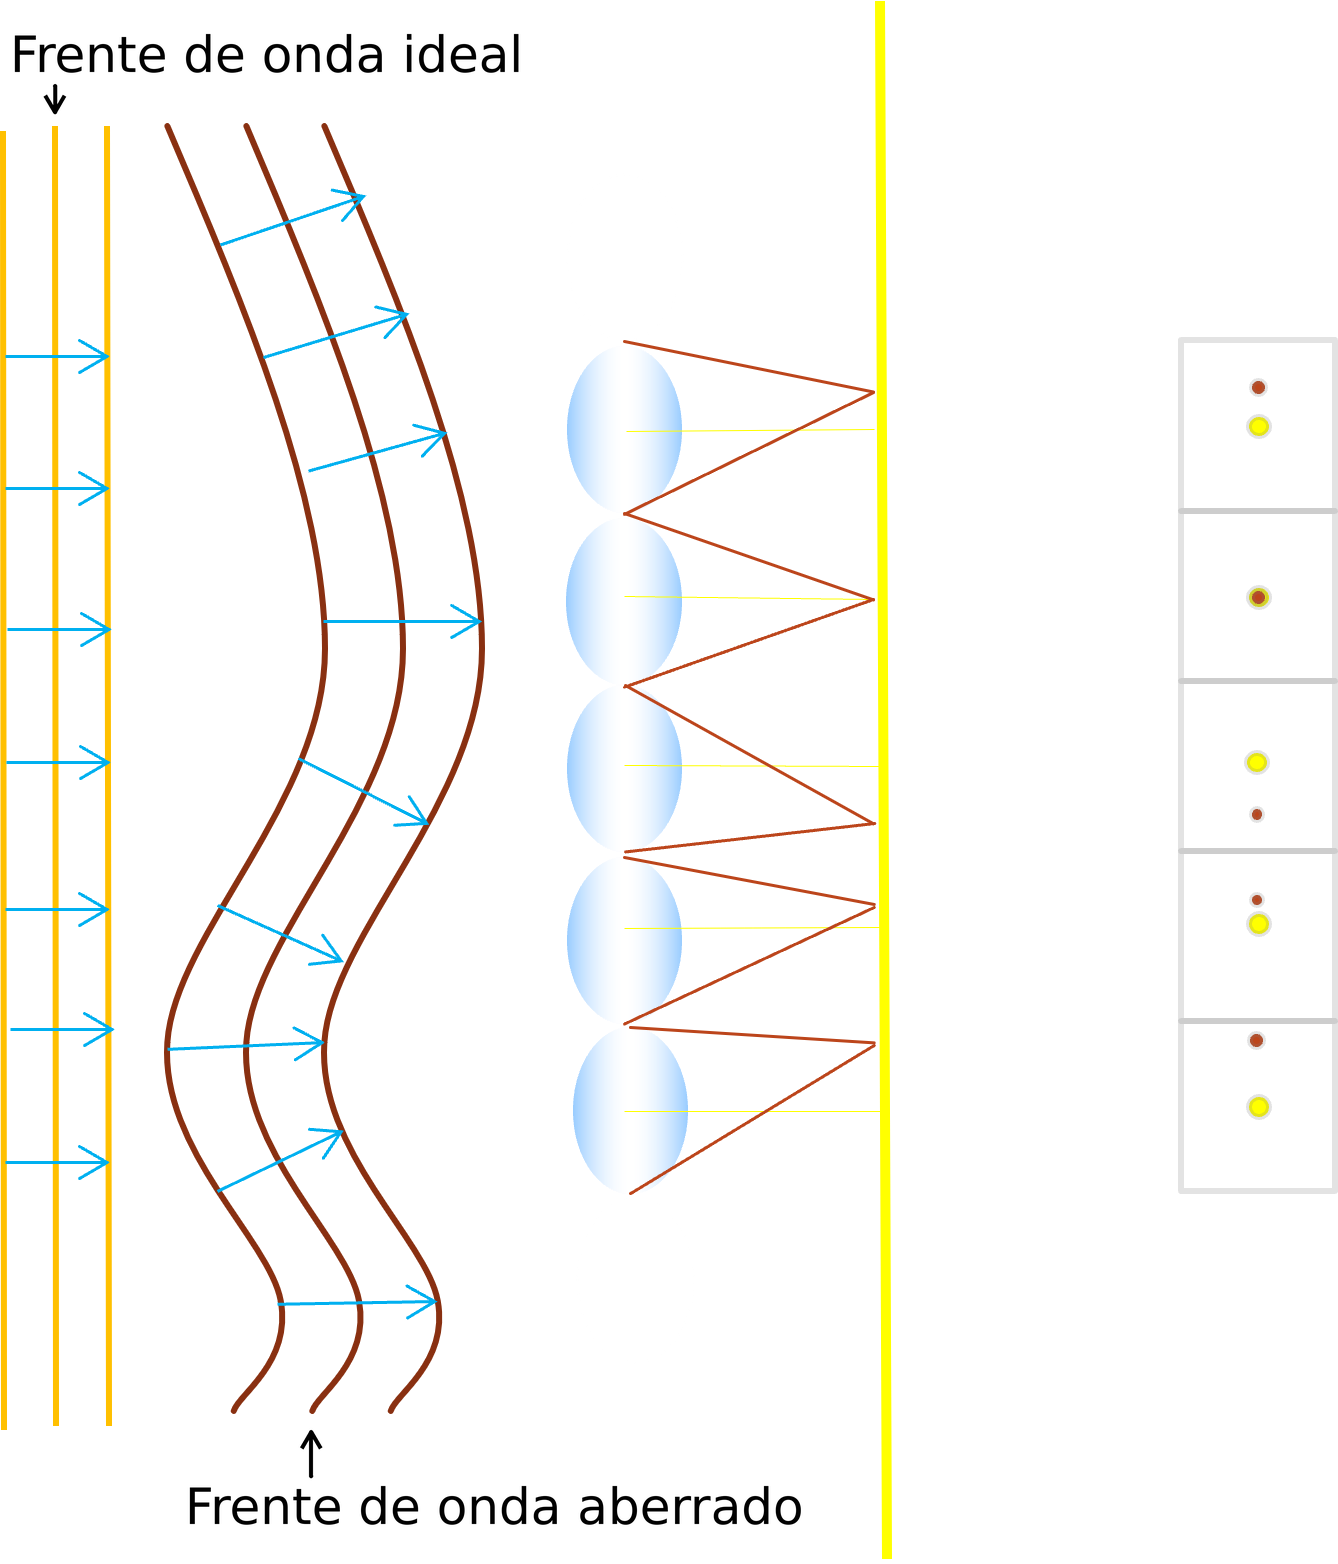
\includegraphics[width=0.5\linewidth]{S-H reoresebtacion-v2.png}
	\caption{Principio de funcionamiento sensor SH, Imagen extraida de \cite{Shack}.}
	\label{fig:s-h}
\end{figure}

Cualquier aberración de fase puede aproximarse mediante un conjunto de inclinaciones
discretas en el sensor de frente de onda Shack-Hartmann. Debido a que solo se miden las
inclinaciones, el método no puede detectar pasos discontinuos en el frente de onda ni el
pistón global, que queda como constante aditiva indeterminada en la reconstrucción.

Otro concepto importante a mencionar es el rango dinámico de un sensor Shack-Hartmann. Éste representa la máxima pendiente del frente de onda que el sensor puede medir sin ambigüedad, expresado típicamente en radianes (rad) \cite{AkondiDubra}. Matemáticamente, en la aproximación de ángulo pequeño ($\tan\alpha \approx \alpha$), se define como
\begin{equation}
\alpha_{max} \approx \frac{P_L}{2\,f_L},
\label{eq:alphamax}
\end{equation}
donde $P_L$ es el paso o distancia entre centros de microlentes adyacentes y $f_L$ es la distancia focal de las microlentes. Esta métrica determina la capacidad del sensor para medir frentes de onda con grandes variaciones locales de pendiente. Cuando la pendiente del frente de onda excede el rango dinámico, las manchas luminosas se desplazan más allá de la región asignada a cada microlente, causando ambigüedades en la asignación de manchas y errores en la reconstrucción del frente de onda \cite{AkondiDubra}. Esta expresión corresponde al límite en el que el tamaño del propio spot es despreciable frente al paso del arreglo ($D_i \ll P_L$); la forma general, que descuenta el diámetro $D_i$ del spot, puede consultarse en \cite{AkondiDubra}. Por tanto, preservar un rango dinámico adecuado es esencial para aplicaciones que involucran la medición de aberraciones ópticas pronunciadas. Como referencia, es conveniente señalar que los métodos interferométricos poseen un rango dinámico reducido, de hasta unas $10$ longitudes de onda ($\sim 5~\mu$m); no obstante, su alta precisión, de hasta $\lambda/1000$ ($\sim 5$~\AA), los convierte en una herramienta muy útil \cite{Greivenkamp}.

\subsection{Técnicas de escaneo en sensores Shack-Hartmann}


En el marco de nuestra investigación, identificamos cinco tipos principales de escaneo. El
primero se describe en el trabajo ``Design and validation of a scanning Shack Hartmann
aberrometer for measurements of the eye over a wide field of view''
\cite{ScanningAberrometer}, donde Wei y Thibos abordan la medición eficiente de las
aberraciones del ojo fuera del eje visual. Para ello incorporan un par de espejos de
escaneo $x$-$y$ que rotan el haz de prueba alrededor del centro de la pupila, permitiendo
que un único sensor Shack-Hartmann fijo capture múltiples líneas de visión en una sola
medición. Este enfoque amplía el campo angular efectivo del aberrómetro sin modificar el
sensor, y se emplea también en otros trabajos de aberrometría ocular.

El segundo método, conocido como Scanning Shack-Hartmann sensor, se utiliza para frentes
de onda divergentes y se describe en el trabajo ``Automated Measurement of Highly
Divergent Optical Wavefronts With a Scanning Shack–Hartmann Sensor''
\cite{FuerstDivergent}. En este caso, el sensor SH se reposiciona y reorienta angularmente
para superar su rango dinámico limitado y medir frentes de onda muy divergentes.

Un tercer enfoque consiste en utilizar un Modulador Espacial de Luz (SLM) para realizar un
``escaneo digital'' del arreglo de microlentes. Este método, propuesto por Guo et al.
\cite{GuoScanning}, reprograma un SLM para generar y desplazar virtualmente el patrón de
lentes difractivas, evitando así el movimiento mecánico y logrando una alta precisión en
el posicionamiento.  En una línea afín, Zhang et al. \cite{ZhangSLM} propusieron
recientemente un sensor basado en un arreglo bidimensional de lentes difractivas de
apertura mixta, orientado a equilibrar el rango dinámico y la resolución espacial.

Otro método importante es la prueba de Hartmann, en la que en lugar de obtener los spots
sobre la superficie o el sistema óptico a través de una pantalla de Hartmann, se utiliza
un haz colimado que recorre el sistema óptico para obtener las pendientes. Este método se
encuentra en el trabajo ``Large-aperture space optical system testing based on the
scanning Hartmann'' \cite{Largespaceopticalsystemtesting,LiuScanning}. Posteriormente, se
propuso una variante de este método con un arreglo de haces colimados llamado ``Multi-beam
array stitching method based on scanning Hartmann for imaging quality evaluation of large
space telescopes'' \cite{WeiMultibeam}.

Finalmente, el quinto tipo corresponde a los sensores Hartmann de apertura extendida de Xu
y Wu, en los que una máscara de Hartmann fija (arreglo de agujeros, no de microlentes) se
combina con un detector que barre el plano de detección: mediante un sensor lineal que
escanea la apertura (\textit{line-scanning}) en \cite{XuExtended}, o mediante un barrido
tipo \textit{raster} con un detector de menor tamaño en \cite{XuRaster}.

El método que se desarrolla en la presente tesis está inspirado en el trabajo de Rufino
Díaz-Uribe, ``Classical Hartmann test with scanning'' \cite{Rufinoangulo}, donde se
propone un sistema de escaneo para la prueba clásica de Hartmann. En este trabajo
adaptamos ese concepto al sensor Shack-Hartmann, desarrollando un sistema de corrimiento
de puntos que permite aumentar la densidad de muestreo bidimensional mediante un único
desplazamiento lineal en un ángulo específico.

Cada uno de estos métodos de escaneo responde a una necesidad específica de medición del
frente de onda.

A diferencia de los métodos basados en elementos difractivos (programables, como el SLM de
Guo et al. \cite{GuoScanning}, o especializados, como el arreglo de apertura mixta de
Zhang et al. \cite{ZhangSLM}), que requieren componentes ópticos adicionales, el enfoque
de corrimiento mecánico que se plantea en esta tesis busca ofrecer una solución más
directa y económica. Al mantener el arreglo físico de microlentes original, se conserva el
paso $P_L$ y la distancia focal $f_L$ del arreglo, parámetros que gobiernan el rango
dinámico geométrico por microlente $\alpha_{max}$ (Ec.~\ref{eq:alphamax}); la resolución
espacial, por su parte, se incrementa mediante el procesamiento conjunto de múltiples
imágenes tomadas con desplazamientos precisos en un ángulo específico. Esta aproximación
se plantea como una vía alternativa para abordar las limitaciones tradicionales del sensor
Shack-Hartmann sin recurrir a componentes ópticos adicionales; su validación cuantitativa
se presenta en el Capítulo 5.


\subsection{Limitaciones actuales}

A pesar de sus numerosas ventajas, los sensores Shack-Hartmann convencionales presentan
ciertas limitaciones. La principal es el compromiso inherente entre resolución espacial,
rango dinámico y sensibilidad \cite{AkondiDubra,GuoScanning}. Para aumentar la resolución
espacial, es necesario incrementar el número de microlentes en el arreglo, lo que implica
reducir el \textit{pitch} entre ellas y, en muchos diseños, también su apertura efectiva.
Esto mejora la densidad de muestreo del frente de onda, pero introduce restricciones
físicas y geométricas bien conocidas.

Por un lado, la mancha focal producida por cada microlente no puede reducirse
indefinidamente, pues su tamaño mínimo está limitado por difracción y depende de la
apertura y la distancia focal de la microlente \cite{Goodman,MalacaraDoblado}. Cuando la
apertura disminuye demasiado, la mancha se ensancha y la localización precisa del
centroide se vuelve más sensible al ruido, a la iluminación no uniforme y a la
discretización del detector; el efecto conjunto de la precisión finita en la determinación
de centroides sobre la reconstrucción del frente de onda fue caracterizado
cuantitativamente mediante simulaciones en~\cite{Takato}.

Por otro lado, reducir el tamaño o el \textit{pitch} de las microlentes disminuye el
desplazamiento máximo admisible del spot antes de invadir la región asignada a una
microlente vecina. En consecuencia, el rango dinámico geométrico por microlente se reduce,
pues la máxima pendiente medible sin ambigüedad depende de la relación entre el
\textit{pitch} y la distancia focal del arreglo \cite{AkondiDubra,FuerstDivergent}. Cuando
esta condición deja de cumplirse, aparecen ambigüedades en la asignación de manchas y
aumenta el riesgo de solapamiento entre spots vecinos \cite{GuoScanning,AkondiDubra}. Este
compromiso entre resolución espacial, sensibilidad y rango dinámico representa un desafío
importante en aplicaciones que requieren medir frentes de onda complejos con alta
fidelidad.

\section{Óptica adaptativa} \label{ch:optica-adaptativa}

La óptica adaptativa es una técnica que permite corregir en tiempo real las aberraciones
ópticas de un sistema, como las causadas por turbulencia atmosférica \cite{TysonAO}. Un
sistema típico consta de un sensor de frente de onda, generalmente Shack-Hartmann, un
espejo deformable y un bucle de control: en cada iteración el sensor mide el frente de
onda y, a partir de esa medición, se actualiza la forma del espejo hasta que el frente que
llega al sensor es plano; el proceso se repite en bucle cerrado cientos de veces por
segundo. En un arreglo de laboratorio como el de la Fig.~\ref{fig:optica-adaptativa}, un
haz láser expandido y colimado atraviesa un plano de muestra, donde puede colocarse el
elemento bajo prueba, incide en el espejo deformable y se releva mediante lentes hasta un
divisor de haz y el sensor. Cuando el bucle converge, el frente de onda bajo prueba se
relaciona con la deformación local del espejo por un factor de $2$ en condiciones de
reflexión próxima a la normal (con incidencia oblicua entra un factor adicional
$\cos\theta_i$) \cite[p.~31 y Anexo~1]{BribiescasTesis}; este punto se retoma en la
Sección~\ref{sec:sistema-optico}.

En este trabajo el kit de óptica adaptativa no se usa para corregir. Su primera parte
sirve únicamente para expandir y colimar el haz sobre el espejo deformable; el plano de
muestra queda vacío y el bucle de corrección no se cierra en ninguna medición. El espejo
deformable actúa como un elemento que genera frentes de onda con fase ajustable
(Sección~\ref{sec:sistema-optico}), y lo que se compara en el
Capítulo~\ref{cap:resultados} es una reconstrucción de ese frente contra otra, no el
desempeño del sistema de óptica adaptativa.

\begin{figure}[htbp] \centering 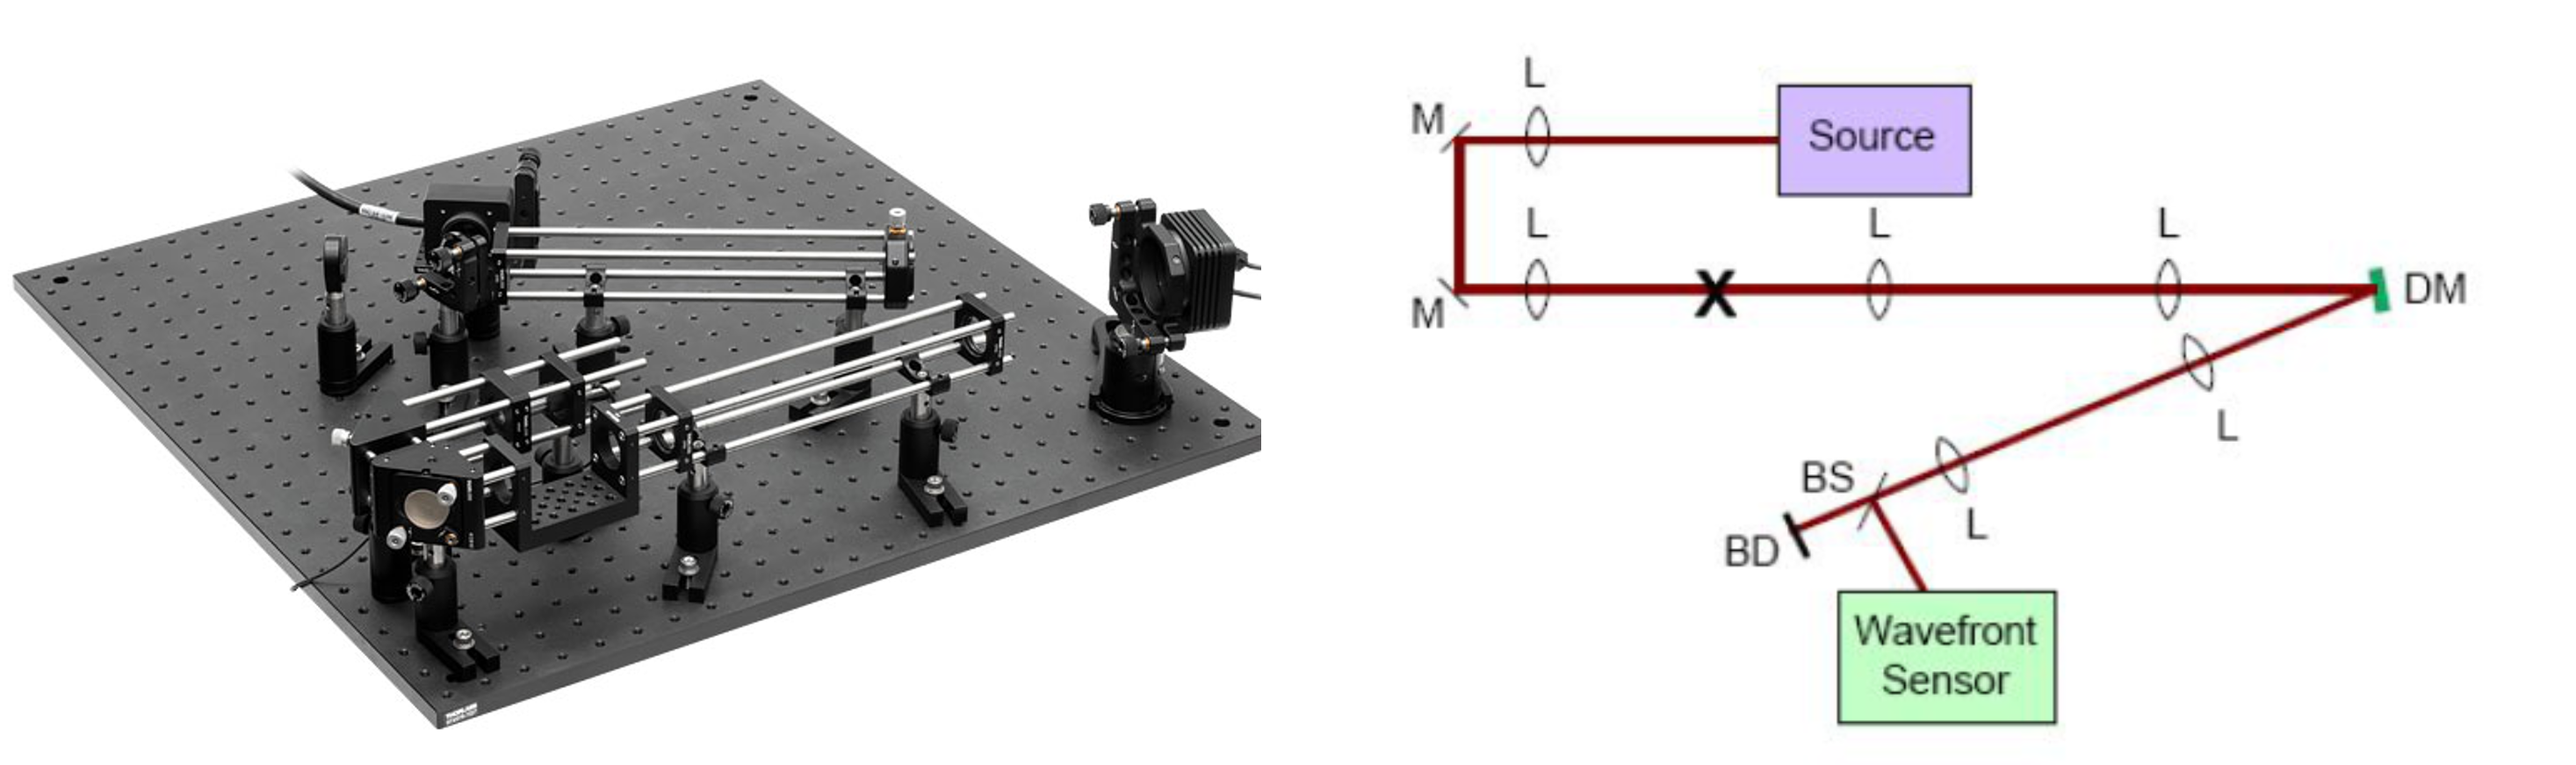
\includegraphics[width=0.85\linewidth]{sitemaOpticaAdaptativa.png} \caption{Diagrama general del kit de óptica adaptativa (tomado del manual del fabricante~\cite{ThorlabsAOKManual}). En este trabajo el plano de muestra queda vacío y el bucle de corrección no se utiliza: el kit sólo expande y colima el haz sobre el espejo deformable.} \label{fig:optica-adaptativa} 
\end{figure}

Aunque en este trabajo se emplea un espejo deformable comercial (modelo DMP40 de Thorlabs,
detallado en el Capítulo 3), sistemas equivalentes pueden construirse en el laboratorio a
partir de sus componentes básicos: una membrana o superficie reflejante, un arreglo de
actuadores y la electrónica de control asociada.

\section{Método de corrimiento de puntos}

El método de corrimiento de puntos (Point Shifting Method) fue originalmente desarrollado
para pruebas ópticas con pantallas nulas \cite{MorenoOliva, RodriguezDyPoS, Rufinoangulo}
y aplicado posteriormente a la evaluación de superficies asféricas mediante pantallas
nulas de prisma cuadrado \cite{ValderramaTesis2020}, donde demostró su eficacia para
aumentar la densidad de puntos de muestreo sin modificar físicamente la pantalla. Este
método consiste en realizar desplazamientos controlados de la pantalla o sensor a lo largo
de direcciones específicas, capturando una imagen diferente en cada posición, lo que
permite obtener información adicional del frente de onda bajo prueba.

En este trabajo se propone adaptar el método de corrimiento de puntos al sensor
Shack-Hartmann con el objetivo de incrementar su densidad transversal de muestreo sin
modificar físicamente el arreglo de microlentes. La hipótesis central es que, al desplazar
el sensor en un ángulo específico y combinar $k$ imágenes, la densidad total de puntos de
medición aumenta de $N$ a $kN$ mientras que el paso $P_L$ y la distancia focal $f_L$ del
arreglo permanecen invariables; en consecuencia, el rango dinámico geométrico por
microlente $\alpha_{max}$ (Ec.~\ref{eq:alphamax}) se conserva. De cumplirse esta
hipótesis, el método permitiría superar el compromiso clásico entre resolución espacial y
rango dinámico del sensor Shack-Hartmann sin requerir modificaciones del hardware ni
componentes ópticos adicionales. La innovación principal radica en el desarrollo
matemático que determina los ángulos óptimos de desplazamiento para garantizar una
distribución final simétrica y uniforme de los puntos de medición; dicho desarrollo se
presenta en el Capítulo 2.

A diferencia de soluciones que proponen reducir el tamaño de las microlentes (estrategia
que incrementa la resolución espacial a costa de disminuir el rango dinámico
$\alpha_{max}$), este enfoque mantiene las dimensiones originales del arreglo y traslada
la ganancia de resolución al procesamiento conjunto de múltiples imágenes desplazadas.
Frente a alternativas como el uso de elementos difractivos \cite{GuoScanning,ZhangSLM} o
esquemas basados en espejos de escaneo \cite{ScanningAberrometer,FuerstDivergent}, la
elección de un corrimiento mecánico se justifica por su simplicidad de implementación y su
compatibilidad directa con el hardware existente del sensor Shack-Hartmann, sin requerir
componentes ópticos adicionales ni programación de fase.

Resultados preliminares de esta investigación han sido ya publicados \cite{SHWS_scan},
demostrando que es posible incrementar significativamente la densidad de puntos de
evaluación mediante este método. En un caso específico, se logró aumentar de 526 a 2641 el
número de puntos de evaluación, manteniendo el rango dinámico original del sensor. Dicha
publicación es un reporte preliminar de los resultados obtenidos en esta tesis, no un
trabajo independiente. Estos resultados preliminares confirman la viabilidad de nuestra
propuesta y justifican el desarrollo detallado que se presenta en esta tesis, en la que se
extienden las evaluaciones a tres configuraciones experimentales que combinan dos modos de
Zernike del espejo deformable ($Z_{11}$ y $Z_{13}$, en la convención de índices del
software de control que se detalla en la Sección~\ref{sec:convencion-zernike}) y dos
factores de densificación ($\varepsilon = 5$ y $\varepsilon = 10$), y se incorpora el
reporte de métricas RMS de error comparadas con la reconstrucción del software de
Thorlabs.

\section{Hipótesis y objetivos}

Como elemento de contexto teórico para las hipótesis que siguen, hay que recordar que la integración por la regla del trapecio empleada tiene un error local acotado \cite{Chapra} por
\begin{equation}
E_k= \frac{1}{12}\left[\frac{\partial^2 f(x,y)}{\partial x^2}\Delta x^3\right]_k,
\label{eq:trapecio}
\end{equation}
donde $\Delta x$ es la distancia entre dos puntos sucesivos a lo largo de la trayectoria de integración y $f(x,y)$ es la forma del frente de onda. La Ec.~\ref{eq:trapecio} expresa el error \emph{local} en cada paso $k$; el error \emph{total} acumulado a lo largo de un camino de integración con $K$ pasos es la suma $E_{\text{total}} = \sum_{k=1}^{K} E_k$ de las contribuciones de cada paso. Esta cota motiva el interés del método: reducir $\Delta x$ mediante la densificación del muestreo abre, en principio, la posibilidad de mejorar la integración numérica en todo el dominio reconstruido.

Las hipótesis que guían este trabajo son:

\begin{enumerate}
	\item \textbf{Premisa central (preservación del rango dinámico):} Dado que el método de corrimiento de puntos no modifica el paso $P_L$ ni la distancia focal $f_L$ del arreglo de microlentes, el rango dinámico geométrico por microlente $\alpha_{max}$ (Ec.~\ref{eq:alphamax}) se conserva por construcción durante todo el proceso, mientras que la densidad total de puntos de muestreo se incrementa de $N$ a $kN$ al combinar $k$ imágenes desplazadas. Esto permite superar el compromiso clásico entre resolución espacial y rango dinámico, un resultado que un arreglo equivalente compuesto por $kN$ microlentes más pequeñas no podría alcanzar sin sacrificar $\alpha_{max}$.

	\item El método de corrimiento de puntos, aplicado sobre el mismo sensor y validado contra la reconstrucción que el software del fabricante produce sobre las mismas mediciones, debe arrojar frentes de onda cuantitativamente comparables a los de la referencia, con una diferencia residual del mismo orden o inferior a la magnitud de las aberraciones bajo prueba.

	\item Se evaluará si el aumento de la densidad muestral introducido por el método de corrimiento de puntos, al reducir el valor de $\Delta x$ y por tanto la cota de error de la Ec.~\ref{eq:trapecio}, se traduce en una mejora cuantificable del error de reconstrucción respecto a la referencia del fabricante en el régimen experimental cubierto. Esta cuestión es de particular interés en frentes de onda con curvaturas no constantes.
\end{enumerate}

Algunas de estas hipótesis han sido ya verificadas en trabajos preliminares
\cite{SHWS_scan}, lo que refuerza la validez de nuestro enfoque y justifica el desarrollo
detallado presentado en esta tesis.

El objetivo general de este trabajo es desarrollar e implementar un método de corrimiento
de puntos aplicado al sensor Shack-Hartmann que permita aumentar la resolución transversal
sin modificar físicamente el arreglo de microlentes.

Los objetivos específicos son:

\begin{itemize}
	\item Desarrollar el fundamento matemático para determinar los ángulos óptimos de desplazamiento que generen distribuciones simétricas bidimensionales.
	\item Diseñar e implementar un sistema experimental que permita el control preciso del desplazamiento del sensor.
	\item Desarrollar algoritmos para el procesamiento e integración de los datos obtenidos de múltiples imágenes.
	\item Evaluar la precisión y resolución del método propuesto mediante la medición de frentes de onda generados de forma controlada por un espejo deformable, comparando cuantitativamente la reconstrucción obtenida contra la del software comercial de Thorlabs aplicado a las mismas mediciones.
\end{itemize}

\section{Estructura de la tesis}

Esta tesis está organizada de la siguiente manera:

\begin{itemize}
	\item  \textbf{El Capítulo 1} presenta el contexto histórico, describe los principios básicos del sensor Shack-Hartmann y la óptica adaptativa, introduce el método de corrimiento de puntos y establece las hipótesis y objetivos del trabajo.
	
	\item \textbf{El Capítulo 2} desarrolla la evaluación por método Shack-Hartmann con corrimiento de puntos, describiendo detalladamente el diseño experimental y el fundamento matemático.
	
	\item  \textbf{El Capítulo 3} presenta el arreglo experimental utilizado, describiendo los componentes y su configuración.
	
	\item  \textbf{El Capítulo 4} detalla la metodología de evaluación, incluyendo el tratamiento de datos y el método de integración numérica.
	
	\item \textbf{El Capítulo 5} muestra los resultados obtenidos y su análisis.
	
	\item \textbf{El Capítulo 6} presenta las conclusiones y perspectivas futuras del trabajo.
\end{itemize}

Esta tesis se basa en una investigación experimental que involucró el diseño y
construcción de un sistema de posicionamiento y adquisición para un sensor de frente de
onda Shack-Hartmann comercial, orientado a la caracterización de frentes de onda generados
por un espejo deformable en un sistema de óptica adaptativa, implementando el método de
corrimiento de puntos para mejorar la resolución transversal, así como la precisión de la
integración de las ecuaciones de Rayces para la reconstrucción del frente de onda.

Se espera que la información presentada en esta tesis sea útil para aquellos que estén
interesados en el diseño y aplicación de sensores de frente de onda Shack-Hartmann, y que
contribuya al avance continuo en el campo de la óptica adaptativa y la fabricación de
componentes ópticos de alta precisión.





\chapter[Evaluación S-H con corrimiento]{Evaluación por método S-H con corrimiento de puntos}

\section{Evaluación clásica Shack-Hartmann}\label{sec:eval-clasica-SH}

Previo a describir el método propuesto, describimos brevemente el flujo clásico de
evaluación con un sensor Shack-Hartmann. Una vez que el frente de onda bajo estudio incide
sobre el arreglo de microlentes, el procedimiento consta de cinco pasos: (1) se captura la
imagen del patrón de spots en el detector, (2) se determinan los centroides de intensidad
de cada spot, (3) se calcula el desplazamiento $(T_x, T_y)$ de cada centroide respecto a
su posición de referencia, es decir, la que ocuparía con un frente de onda plano, (4) cada
componente del desplazamiento se convierte en una pendiente local del frente de onda
mediante la siguiente ecuación (Ec.~\ref{eq:pendiente-local-cap2}),

\begin{equation}
\alpha_x \approx \frac{T_x}{f_L}, \qquad \alpha_y \approx \frac{T_y}{f_L},
\label{eq:pendiente-local-cap2}
\end{equation}
válida en la aproximación de ángulo pequeño ($\tan\alpha \approx \alpha$), que se cumple para las pendientes dentro del rango dinámico del sensor, y (5) las pendientes así obtenidas se integran numéricamente para reconstruir el frente de onda completo \cite{Malacara, AkondiDubra}.

Para formalizar las magnitudes que entran al paso (4) del flujo anterior, se define la \textbf{aberración transversal} en cada microlente como el desplazamiento del centroide medido respecto al centro geométrico de la microlente:
\begin{equation}
T_x = x_\ell - x_c, \qquad T_y = y_\ell - y_c,
\label{eq:aberracion-transversal-cap2}
\end{equation}
donde $(x_c, y_c)$ es la posición medida del centroide y $(x_\ell, y_\ell)$ es el centro geométrico de la microlente, que no se mide sino que queda fijado por el paso $P_L$ del arreglo; ambos se expresan en el mismo sistema de coordenadas espaciales. En ausencia de aberración el centroide cae sobre el centro de la microlente y $(T_x, T_y) = (0, 0)$. La Fig.~\ref{fig:aberracion-transversal-cap2} ilustra esta magnitud: un frente de onda aberrado desplaza el centroide de cada microlente respecto a la posición de referencia que ocuparía con un frente de onda plano, y ese desplazamiento se descompone en las componentes $T_x$ y $T_y$ sobre el plano del detector.

\begin{figure}[htbp]
  \centering
  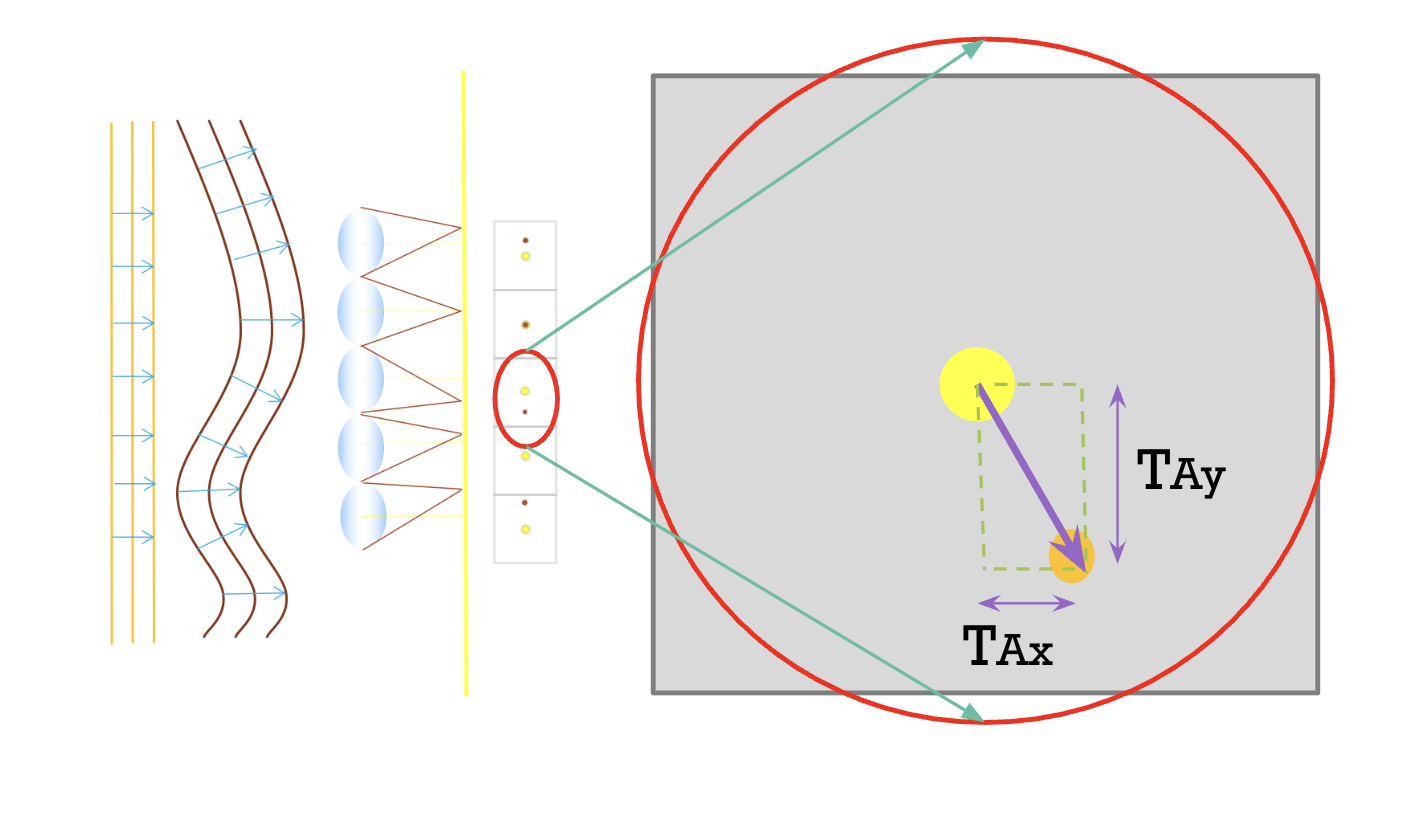
\includegraphics[width=0.95\linewidth]{cap2-aberracion-transversal.png}
  \caption{Aberración transversal en el sensor Shack-Hartmann. \textbf{Izquierda}: un
  frente de onda plano (líneas amarillas) y uno aberrado (líneas cafés) inciden sobre el
  arreglo de microlentes; cada microlente enfoca una mancha sobre el plano del detector,
  donde se registran la posición de referencia (punto amarillo) y el centroide medido
  (punto oscuro). \textbf{Derecha}: acercamiento a una celda del detector; el
  desplazamiento del centroide medido respecto a la referencia (flecha) se descompone en
  las componentes $T_{Ax}$ y $T_{Ay}$, que corresponden a $(T_x, T_y)$ de la
  Ec.~\ref{eq:aberracion-transversal-cap2}.}
  \label{fig:aberracion-transversal-cap2}
\end{figure}

La pendiente local del frente de onda en la microlente se relaciona con la aberración transversal (Ec.~\ref{eq:pendiente-local-cap2}) y, en términos del frente de onda $W$, se escribe:
\begin{equation}
 \frac{\partial W}{\partial x} \approx \frac{T_x}{f_L}, \qquad \frac{\partial W}{\partial y} \approx \frac{T_y}{f_L}.
\label{eq:pendiente-aberracion-cap2}
\end{equation}

La integración numérica de estas pendientes (paso 5) reconstruye el frente de onda salvo
una constante de pistón. La implementación concreta de este flujo en el contexto del
método de corrimiento de puntos se desarrolla en el Capítulo~\ref{cap:metodologia}.

\section{Diseño}

Respecto al flujo clásico de la Sección~\ref{sec:eval-clasica-SH}, el método de
corrimiento de puntos modifica únicamente el paso (1), la captura: en lugar de una sola
imagen se adquieren $k$ imágenes con desplazamientos controlados del sensor, y los pasos
(2) a (5) se aplican al patrón compuesto de $kN$ puntos resultante. El frente de onda bajo
prueba puede ser cualquiera; en este trabajo lo genera el espejo deformable del montaje
(Sección~\ref{sec:sistema-optico}).

El propósito del experimento es implementar el corrimiento de puntos en una prueba óptica
tipo Shack-Hartmann para muestrear más puntos del frente de onda. Para este propósito, se
pueden plantear diferentes formas, por ejemplo, desplazar el arreglo de microlentes en las
direcciones principales de las lentes sobre el mismo plano con control micrométrico. Sin
embargo, esto genera diferentes problemas debido a que se introducen dos grados de
libertad en el control biaxial del arreglo, ya que se requieren dos datos por medición (el
desplazamiento en cada una de las dos direcciones).

Por lo anterior, se utiliza un método que permita generar un muestreo denso del arreglo a
partir únicamente del desplazamiento en una dirección. La propuesta fue realizada por
Rufino Díaz en su trabajo \cite{Rufinoangulo}. Para conseguir esto, se rota de forma
calculada el arreglo de microlentes y se generan desplazamientos que ayudan a crear un
patrón final más denso de puntos, como se muestra en la Fig.~\ref{fig:rotacion} b).

\begin{figure}[htbp!]
	\centering
	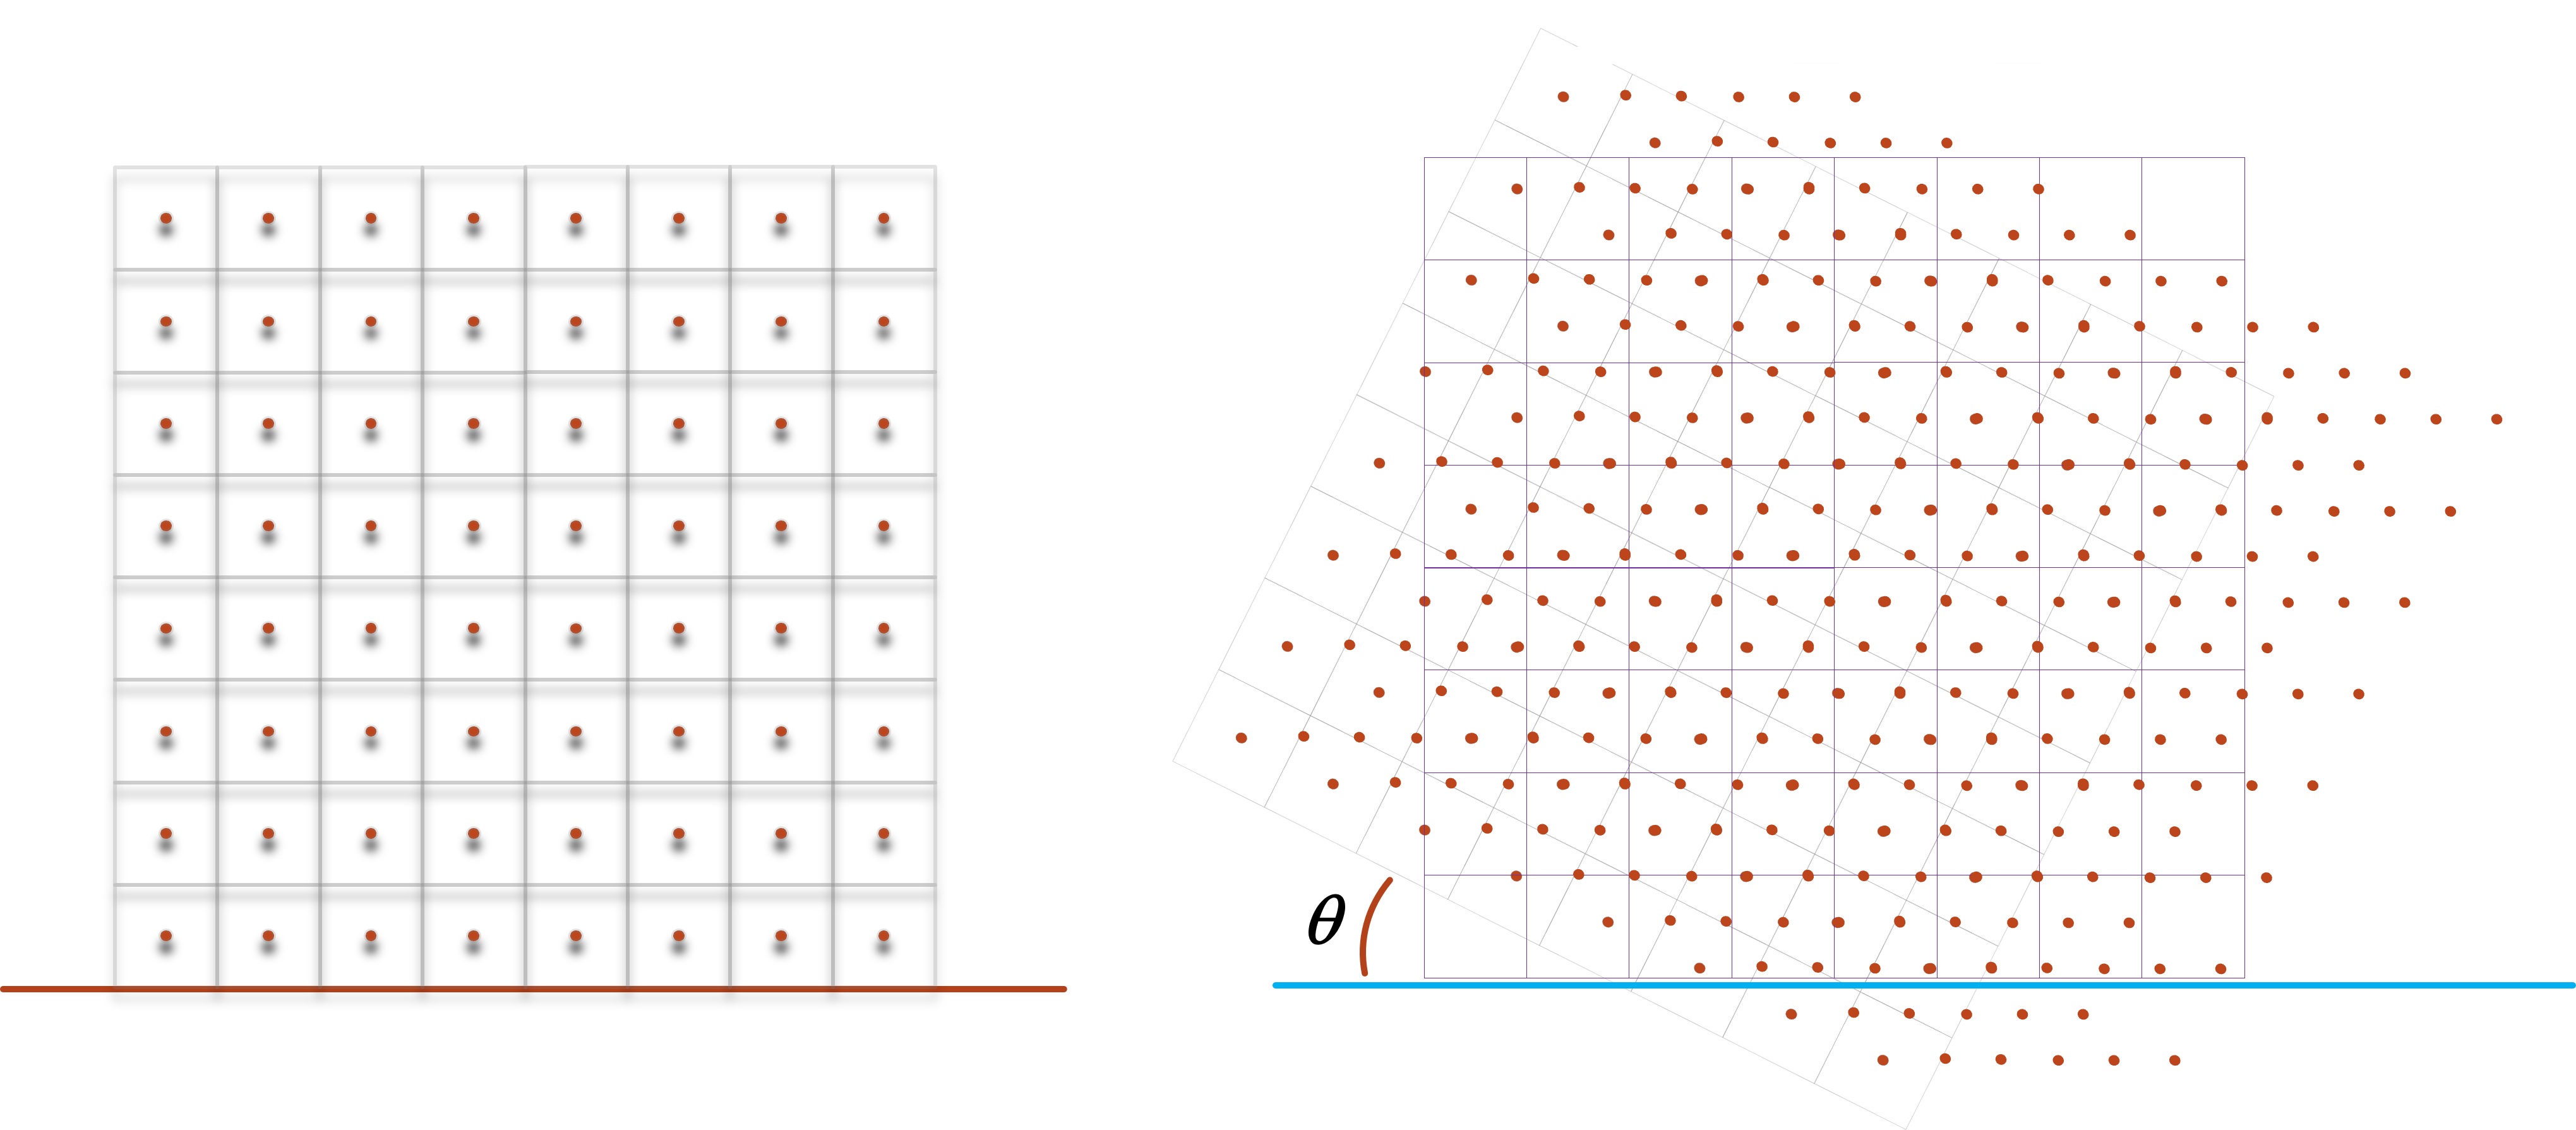
\includegraphics[width=0.8\linewidth]{Rotacion.png}
	\caption{Ejemplo de rotación de arreglo de microlentes}
	\label{fig:rotacion}
\end{figure}

El ángulo de rotación $\theta_r$ debe escogerse de modo que la dirección del
desplazamiento pase periódicamente por los centros de microlentes del arreglo. Para
formalizar esta condición introducimos un sistema de coordenadas asociado a la retícula:
sus dos \textbf{direcciones principales}, que llamaremos $M$ (vertical) y $N$
(horizontal), coinciden con los ejes del arreglo periódico cuadrado de microlentes, y la
unidad de distancia se toma como el paso o separación entre centros de lentes adyacentes
($P_L$, \textit{pitch}). En este sistema, el centro de cualquier microlente queda
identificado por un par de enteros $(m,n)$, donde $m$ cuenta el número de lentes a lo
largo de $M$ y $n$ a lo largo de $N$. Elegir un par concreto $(m,n)$ cumple un doble
propósito: identifica simultáneamente (i) la \emph{microlente objetivo} y (ii) la
dirección del desplazamiento del sensor. La microlente objetivo es aquella vecina de la
microlente de partida cuyo centro se alcanza al completar los $\varepsilon$ corrimientos:
la distancia total recorrida iguala exactamente la separación entre la microlente de
partida y dicha vecina, de modo que un corrimiento adicional reproduciría el patrón
original de puntos. Esta condición de cierre es la que garantiza que las $\varepsilon$
posiciones intermedias se repartan de forma periódica y homogénea sobre la retícula. La
condición involucra únicamente la dirección y el paso de la traslación: en el montaje, la
rotación que fija $\theta_r$ se realiza una sola vez antes del barrido y el sensor no
vuelve a girar durante las $\varepsilon$ capturas, de modo que un eje de giro que no pase
por el centro del arreglo sólo traslada el arreglo completo en una cantidad constante, sin
efecto sobre el cierre; una inclinación residual del plano del sensor respecto al haz
(cabeceo) no altera la retícula y se manifiesta como una inclinación global del frente de
onda reconstruido, que se trata en la Sección~\ref{sec:comparacion}. El ángulo de rotación
necesario para alinear el eje de traslación con la microlente objetivo, medido desde la
dirección horizontal $N$, se obtiene como:

\begin{equation}
\theta_r = \arctan\!\left(\frac{m}{n}\right), \qquad (m,n) \in \mathbb{Z}^2 \setminus \{(0,0)\}, \quad \mcd(m,n) = 1
\label{Eq: angulo}
\end{equation}

donde la condición $\mcd(m,n)=1$ (Máximo Común Divisor, MCD, igual a uno: primos
relativos) garantiza que cada par defina una dirección única; por ejemplo, $(2,4)$
apuntaría en la misma dirección que $(1,2)$ y por eso se descarta. Sin pérdida de
generalidad, basta considerar pares con $m, n > 0$, ya que la simetría cuadrada del
arreglo hace que los demás cuadrantes generen rotaciones equivalentes. Por la misma
simetría, asignar el papel de $M$ a una dirección u otra es convencional: las
orientaciones $\arctan(m/n)$ y $\arctan(n/m)$ describen reticulados densificados
equivalentes, intercambiados por una rotación de $90^\circ$. Aquí se adopta $\arctan(m/n)$
por consistencia con la implementación numérica empleada en el
Capítulo~\ref{cap:metodologia} y con los valores reportados durante el alineamiento del
montaje.

\begin{figure}[htbp!]
	\centering
	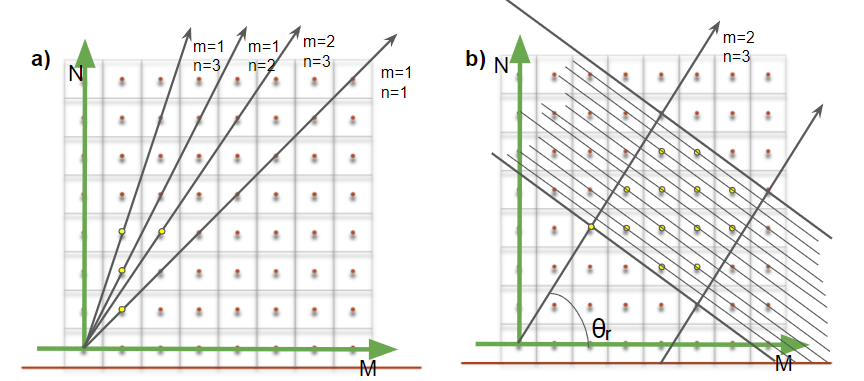
\includegraphics[width=0.9\linewidth]{Img_rotacion-v2.png}
	\caption{Imagen representativa, a) direcciones de barrido, b) número de corrimientos para
	ese ángulo de barrido.}
	\label{fig:imgrotacion}
\end{figure}


Una vez elegido el ángulo de rotación mediante la Ec.~\ref{Eq: angulo}, se asegura que la
dirección del desplazamiento pase por los centros de dos lentes del arreglo inicial. Esto
permite determinar con precisión la distancia entre estos puntos, que corresponde a
$\sqrt{m^2+n^2}$ veces la distancia entre lentes adyacentes en las direcciones
principales. El siguiente paso es subdividir este espacio de forma equitativa para obtener
un arreglo de puntos con distancias iguales, que se replicará a lo largo de todo el
sensor.

Sin embargo, si esta subdivisión se realiza arbitrariamente, la mayor parte de estas
divisiones generarán un patrón desordenado. En muchos casos, si se eligen mal los
espaciamientos, las distancias en la dirección vertical quedarán más pequeñas que las de
la dirección horizontal sobre el plano de las lentes, como se muestra en la
Fig.~\ref{fig:divisiones} a). Para obtener un patrón rectangular de puntos con
espaciamiento uniforme, se encontró que es necesario elegir un número específico de
particiones $\varepsilon$.

\begin{figure}[htbp!]
	\centering
	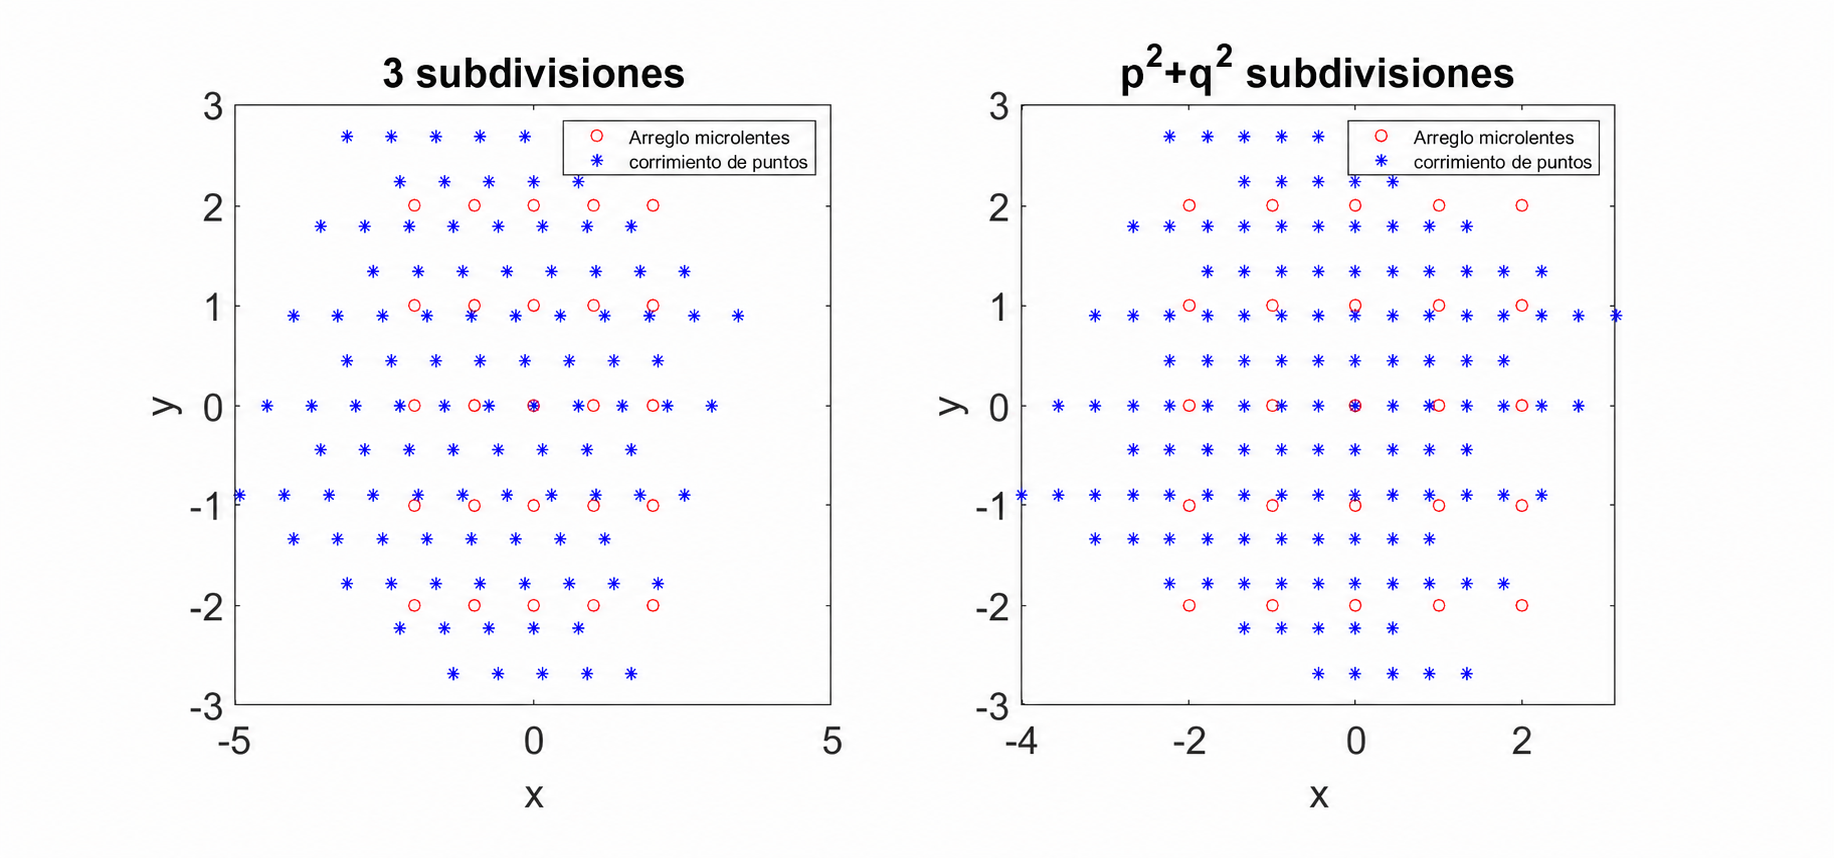
\includegraphics[width=.8\linewidth]{Divisiones2.png}
	\caption{Ejemplo de corrimientos, con $m=1$, $n=1$}
	\label{fig:divisiones}
\end{figure}

Para determinar este número óptimo de particiones, se analiza la geometría del arreglo. A
partir de ${m,n} \neq 0$ y conociendo la posición de la siguiente lente en esa dirección
$(m,n)$, se traza una línea en la dirección perpendicular, que quedará en la dirección
(-n,m), como se muestra en la Fig.~\ref{fig:imgrotacion}b. Dado que los vectores $(m,n)$ y
$(-n,m)$ son perpendiculares y de igual magnitud $\sqrt{m^2+n^2}$, estas dos direcciones
forman un cuadrado cuyos vértices coinciden exactamente con centros de lentes. Cerrando
este cuadrado con líneas paralelas, se define una región donde las lentes contenidas no
coincidirán con ninguna otra línea de desplazamiento, lo que determina el número de
particiones necesarias en la dirección elegida. Este número es igual al área de la región
cuadrada enmarcada por las líneas y se calcula como:

\begin{equation}
\varepsilon = \sqrt{(m^2+n^2)}^2=m^2+n^2
\end{equation}

Así se garantiza la uniformidad en la distribución muestral del frente de onda, de manera
que se pueda tener el mismo margen de error en ambas direcciones, obteniendo un arreglo
regular como el mostrado en la Fig.~\ref{fig:divisiones} b), con una distancia por
corrimiento $\sigma$ igual a:

\begin{equation}
\sigma=\frac{P_L}{\sqrt{\varepsilon}},
\label{eq:distdesp}
\end{equation}

donde $P_L$ es el paso del arreglo (\textit{pitch}) y $\varepsilon$ es el número de
corrimientos.

En la práctica, este proceso puede abordarse también de manera inversa. Es posible
determinar primero el número de desplazamientos deseados, basándose en cuánto se quiere
aumentar la densidad de puntos o en el tamaño de paso aproximado que se requiere para una
aplicación específica. A partir de este número de particiones objetivo, se pueden
seleccionar valores de $m$ y $n$ que sean primos relativos entre sí y cuya suma de
cuadrados ($m^2 + n^2$) sea igual o se aproxime al número de corrimientos deseado. Una vez
determinados estos valores, se obtiene el ángulo $\theta_r$ mediante la Ec.~\ref{Eq:
angulo}. Este enfoque práctico permite adaptar el método a las necesidades específicas de
cada experimento, optimizando la relación entre el aumento de la densidad de muestreo y la
complejidad operativa.

La Tabla~\ref{tab:mn-configuraciones} resume, para los primeros pares $(m,n)$ admisibles,
el ángulo de rotación, el número de corrimientos y el paso resultante, calculados con las
Ecs.~\ref{Eq: angulo} y \ref{eq:distdesp} para el paso $P_L = 0.150$~mm del arreglo
utilizado en este trabajo. El paso por corrimiento $\sigma = P_L/\sqrt{\varepsilon}$
coincide con la separación efectiva entre puntos vecinos del reticulado densificado.

\begin{table}[htbp]
\centering
\caption{Configuraciones de barrido para los primeros pares $(m,n)$ con $\mcd(m,n)=1$:
ángulo de rotación $\theta_r$, número de corrimientos $\varepsilon = m^2+n^2$ y paso por
corrimiento $\sigma = P_L/\sqrt{\varepsilon}$ (para $P_L = 0.150$~mm). Las dos
configuraciones marcadas son las empleadas en las evaluaciones del
Capítulo~\ref{cap:resultados}.}
\label{tab:mn-configuraciones}
\begin{tabular}{ccccl}
\hline
$\boldsymbol{(m,n)}$ & $\boldsymbol{\theta_r}$ & $\boldsymbol{\varepsilon}$ & $\boldsymbol{\sigma}$ \textbf{(mm)} & \textbf{Uso en este trabajo} \\
\hline
$(1,1)$ & $45.00^\circ$ & $2$  & $0.1061$ & --- \\
$(1,2)$ & $26.57^\circ$ & $5$  & $0.0671$ & Evaluaciones 1 y 2 \\
$(1,3)$ & $18.43^\circ$ & $10$ & $0.0474$ & Evaluación 3 \\
$(2,3)$ & $33.69^\circ$ & $13$ & $0.0416$ & --- \\
$(1,4)$ & $14.04^\circ$ & $17$ & $0.0364$ & --- \\
\hline
\end{tabular}
\end{table}



\section{Procedimiento experimental}

A partir del diseño geométrico desarrollado en la sección anterior, el procedimiento de
evaluación con corrimiento de puntos consta de seis pasos conceptuales:

\begin{enumerate}
	\item Elegir un par de índices $(m,n)$ con $\mcd(m,n)=1$ que defina la dirección de barrido y, mediante la Ec.~\ref{Eq: angulo} y la relación $\varepsilon = m^2+n^2$, determinar el ángulo de rotación $\theta_r$ y el número de corrimientos requeridos.

	\item Rotar el sensor en torno a su eje óptico hasta alinearlo con la dirección $\theta_r$ calculada. Como sólo importa la \emph{dirección}, es decir, la recta definida por $\theta_r$ y no el sentido en que se recorre, es indistinto trabajar con $\theta_r$ o $\theta_r+180^\circ$, lo que permite aprovechar la geometría natural del montaje. Como nota práctica, rotar el sensor puede modificar su altura respecto al plano del haz, por lo que el método admite (aunque no requiere intrínsecamente) una mesa de altura variable como ajuste auxiliar.

	\item Alinear el haz incidente para que llegue centrado al sensor.

	\item Generar un frente de onda bajo prueba. En este trabajo se obtiene con el espejo deformable del kit de óptica adaptativa (Sección~\ref{sec:sistema-optico}); no necesita conocerse en sentido absoluto porque la validación del método es relativa (Sección~\ref{sec:comparacion}).

	\item Adquirir un conjunto de centroides en cada una de las $\varepsilon$ posiciones de corrimiento del sensor a lo largo de la dirección $\theta_r$, con un paso $\sigma$ dado por la Ec.~\ref{eq:distdesp}.

	\item Componer los $\varepsilon$ conjuntos de centroides en un único patrón densificado, sobre el que se aplica la reconstrucción numérica del frente de onda.
\end{enumerate}

La implementación concreta de estos pasos (el equipo utilizado, los ajustes mecánicos
secundarios y el procesamiento de los datos) se describe en detalle en el
Capítulo~\ref{cap:metodologia}.








\chapter{Arreglo experimental}

En este capítulo se presenta en detalle el arreglo experimental utilizado para llevar a
cabo las mediciones mediante el método Shack-Hartmann con corrimiento de puntos. El
objetivo principal de este sistema es permitir la caracterización de frentes de onda
ópticos con mayor resolución espacial sin comprometer el rango dinámico del sensor.

El arreglo experimental integra diversos componentes ópticos, mecánicos y electrónicos que
trabajan conjuntamente para lograr mediciones precisas. Los elementos fundamentales
incluyen: (1) el sensor Shack-Hartmann (Fig.~\ref{fig:sh-sensor}), que proporciona las
mediciones básicas de la pendiente local del frente de onda; (2) un sistema de
posicionamiento angular y lineal de alta precisión (Figs.~\ref{fig:sistema-angular}
y~\ref{fig:sistema-optico}), que permite realizar el corrimiento controlado del sensor;
(3) un sistema óptico adaptativo basado en un espejo deformable
(Figs.~\ref{fig:espejo-deformable-MP} y~\ref{fig:optica-adaptativa}), que genera los
frentes de onda de prueba; y (4) un sistema de control y adquisición de datos que gestiona
todos estos componentes (Sección~\ref{sec:control-adquisicion}).

En particular, se describen los elementos utilizados para el control y movilidad del
sensor Shack-Hartmann, así como el sistema empleado para generar el frente de onda bajo
prueba.

\section{Visión general del sistema}

El arreglo experimental desarrollado para este trabajo integra múltiples subsistemas que
funcionan coordinadamente para implementar el método de corrimiento de puntos en un sensor
Shack-Hartmann. La Fig.~\ref{fig:sistema-optico} muestra el sistema montado en
laboratorio, donde se pueden apreciar los componentes principales y su disposición física.

\begin{figure}[H]
	\centering
	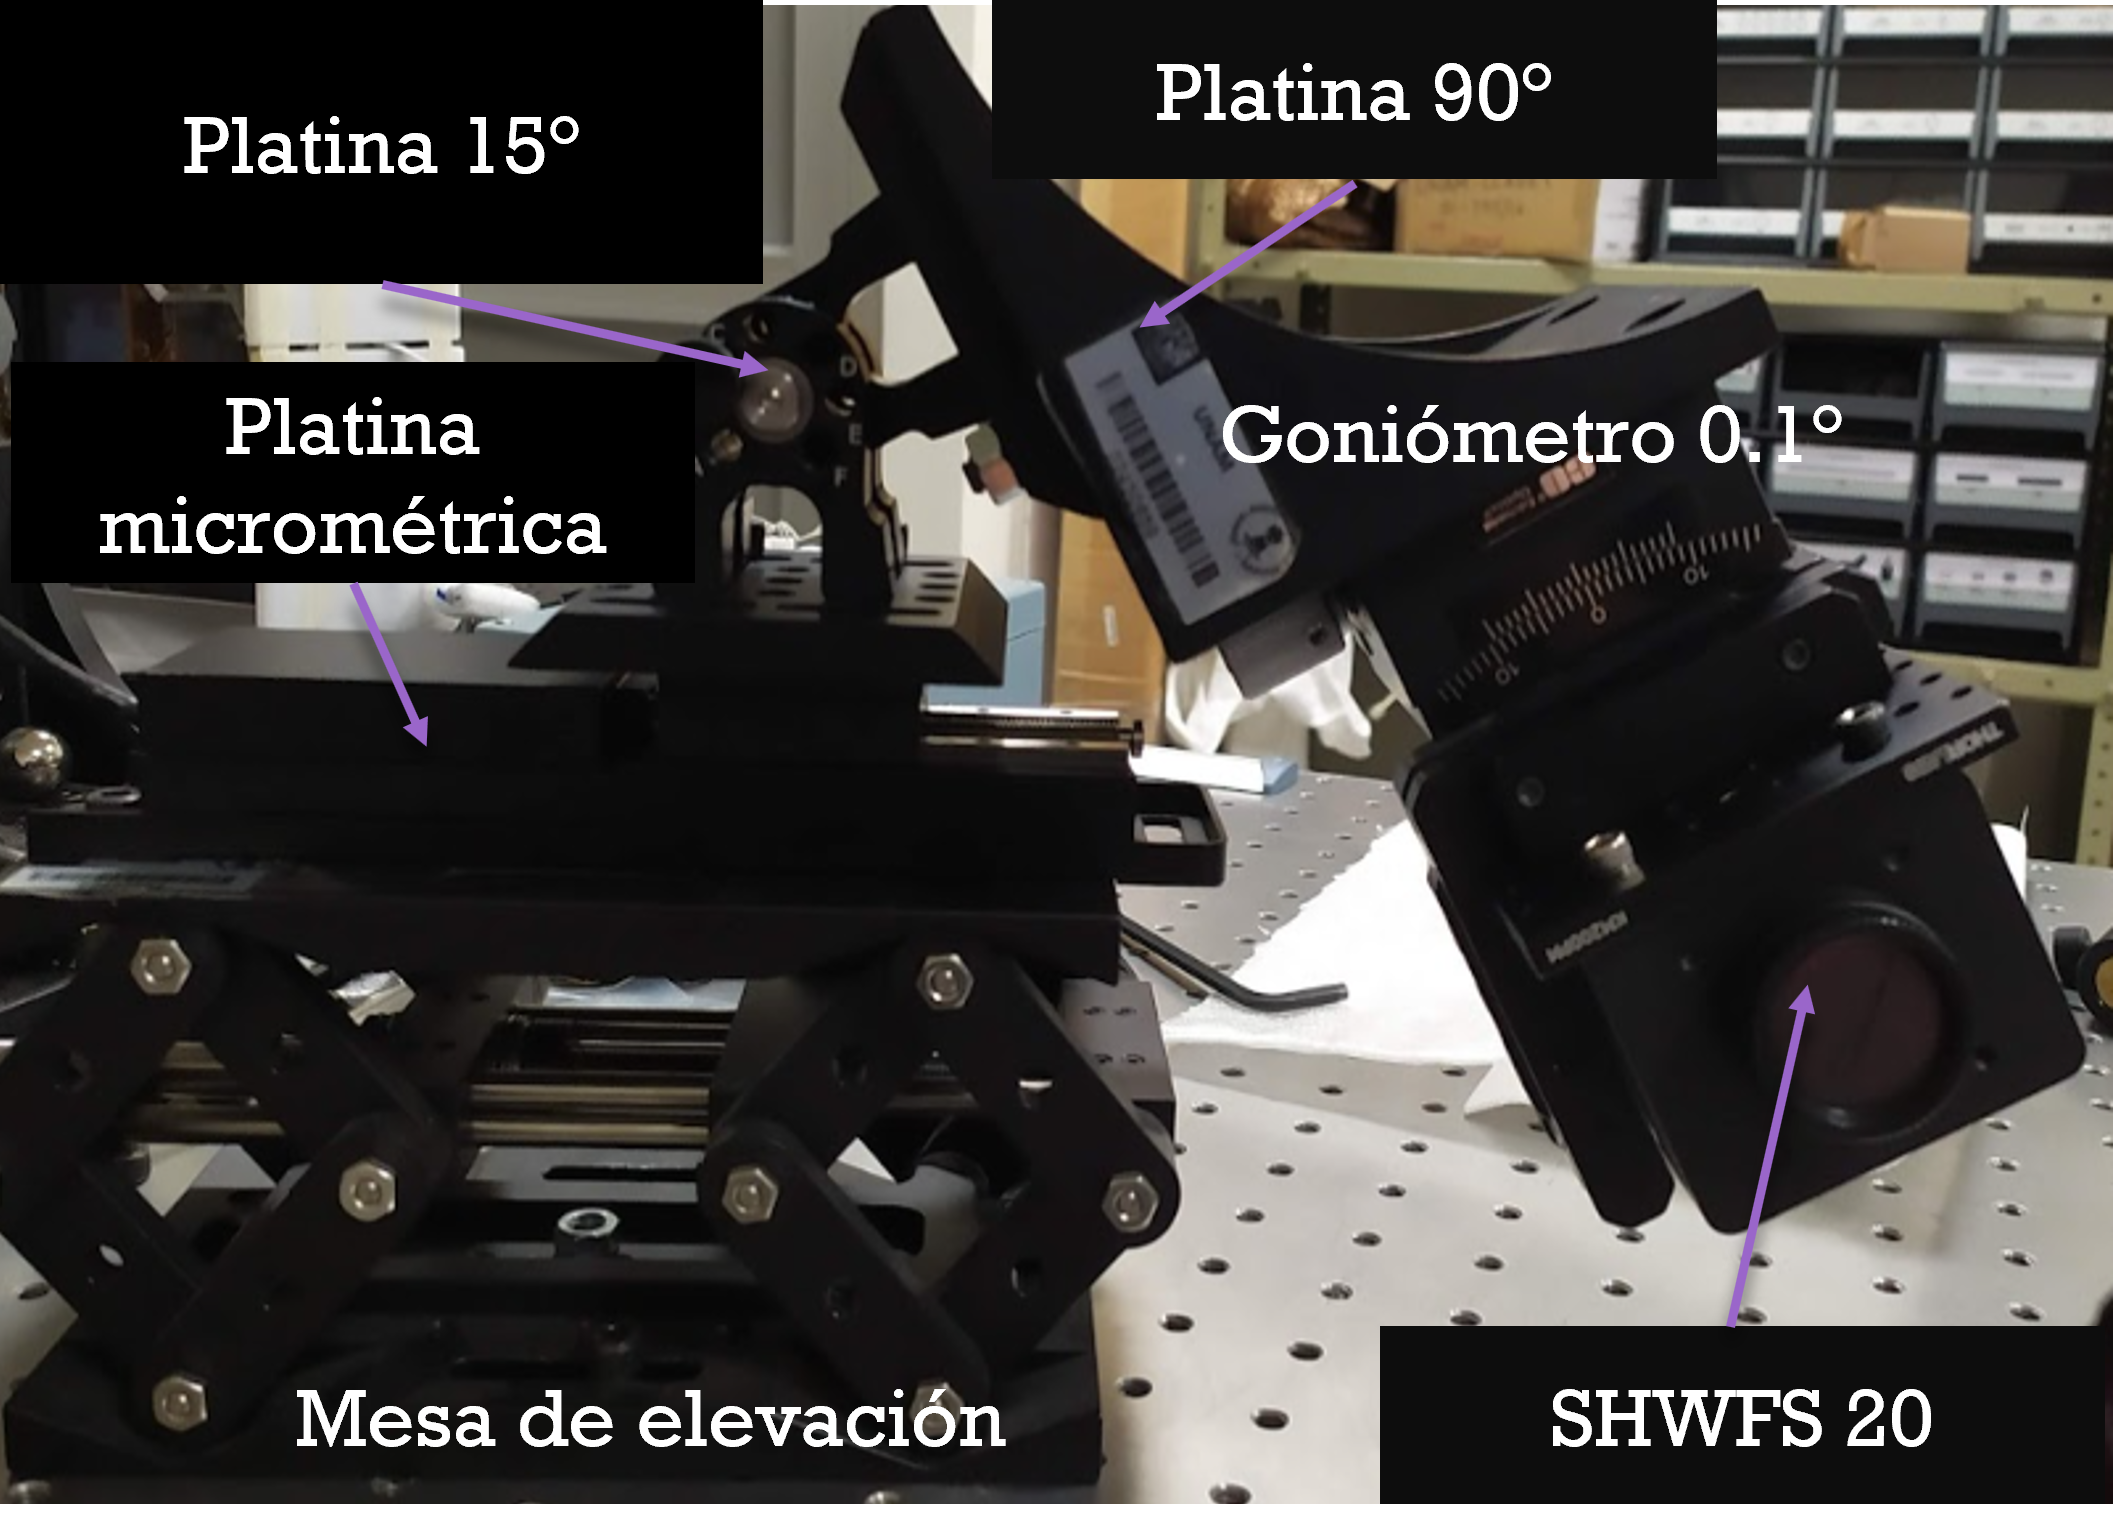
\includegraphics[width=0.6\linewidth]{sistema optico.png}
	\caption{Sensor Shack-Hartmann y montaje en sistema de control espacial}
	\label{fig:sistema-optico}
\end{figure}

El flujo de trabajo del sistema comienza con la generación de un haz láser colimado que se
refleja en el espejo deformable, donde se modifica intencionalmente para crear un frente
de onda aberrado de forma controlada. Este frente de onda es dirigido hacia el sensor
Shack-Hartmann, montado sobre un sistema de posicionamiento de alta precisión que permite
desplazamientos tanto angulares como lineales. La Fig.~\ref{fig:foto-montaje} muestra el
montaje real sobre la mesa óptica.

\begin{figure}[htbp]
	\centering
	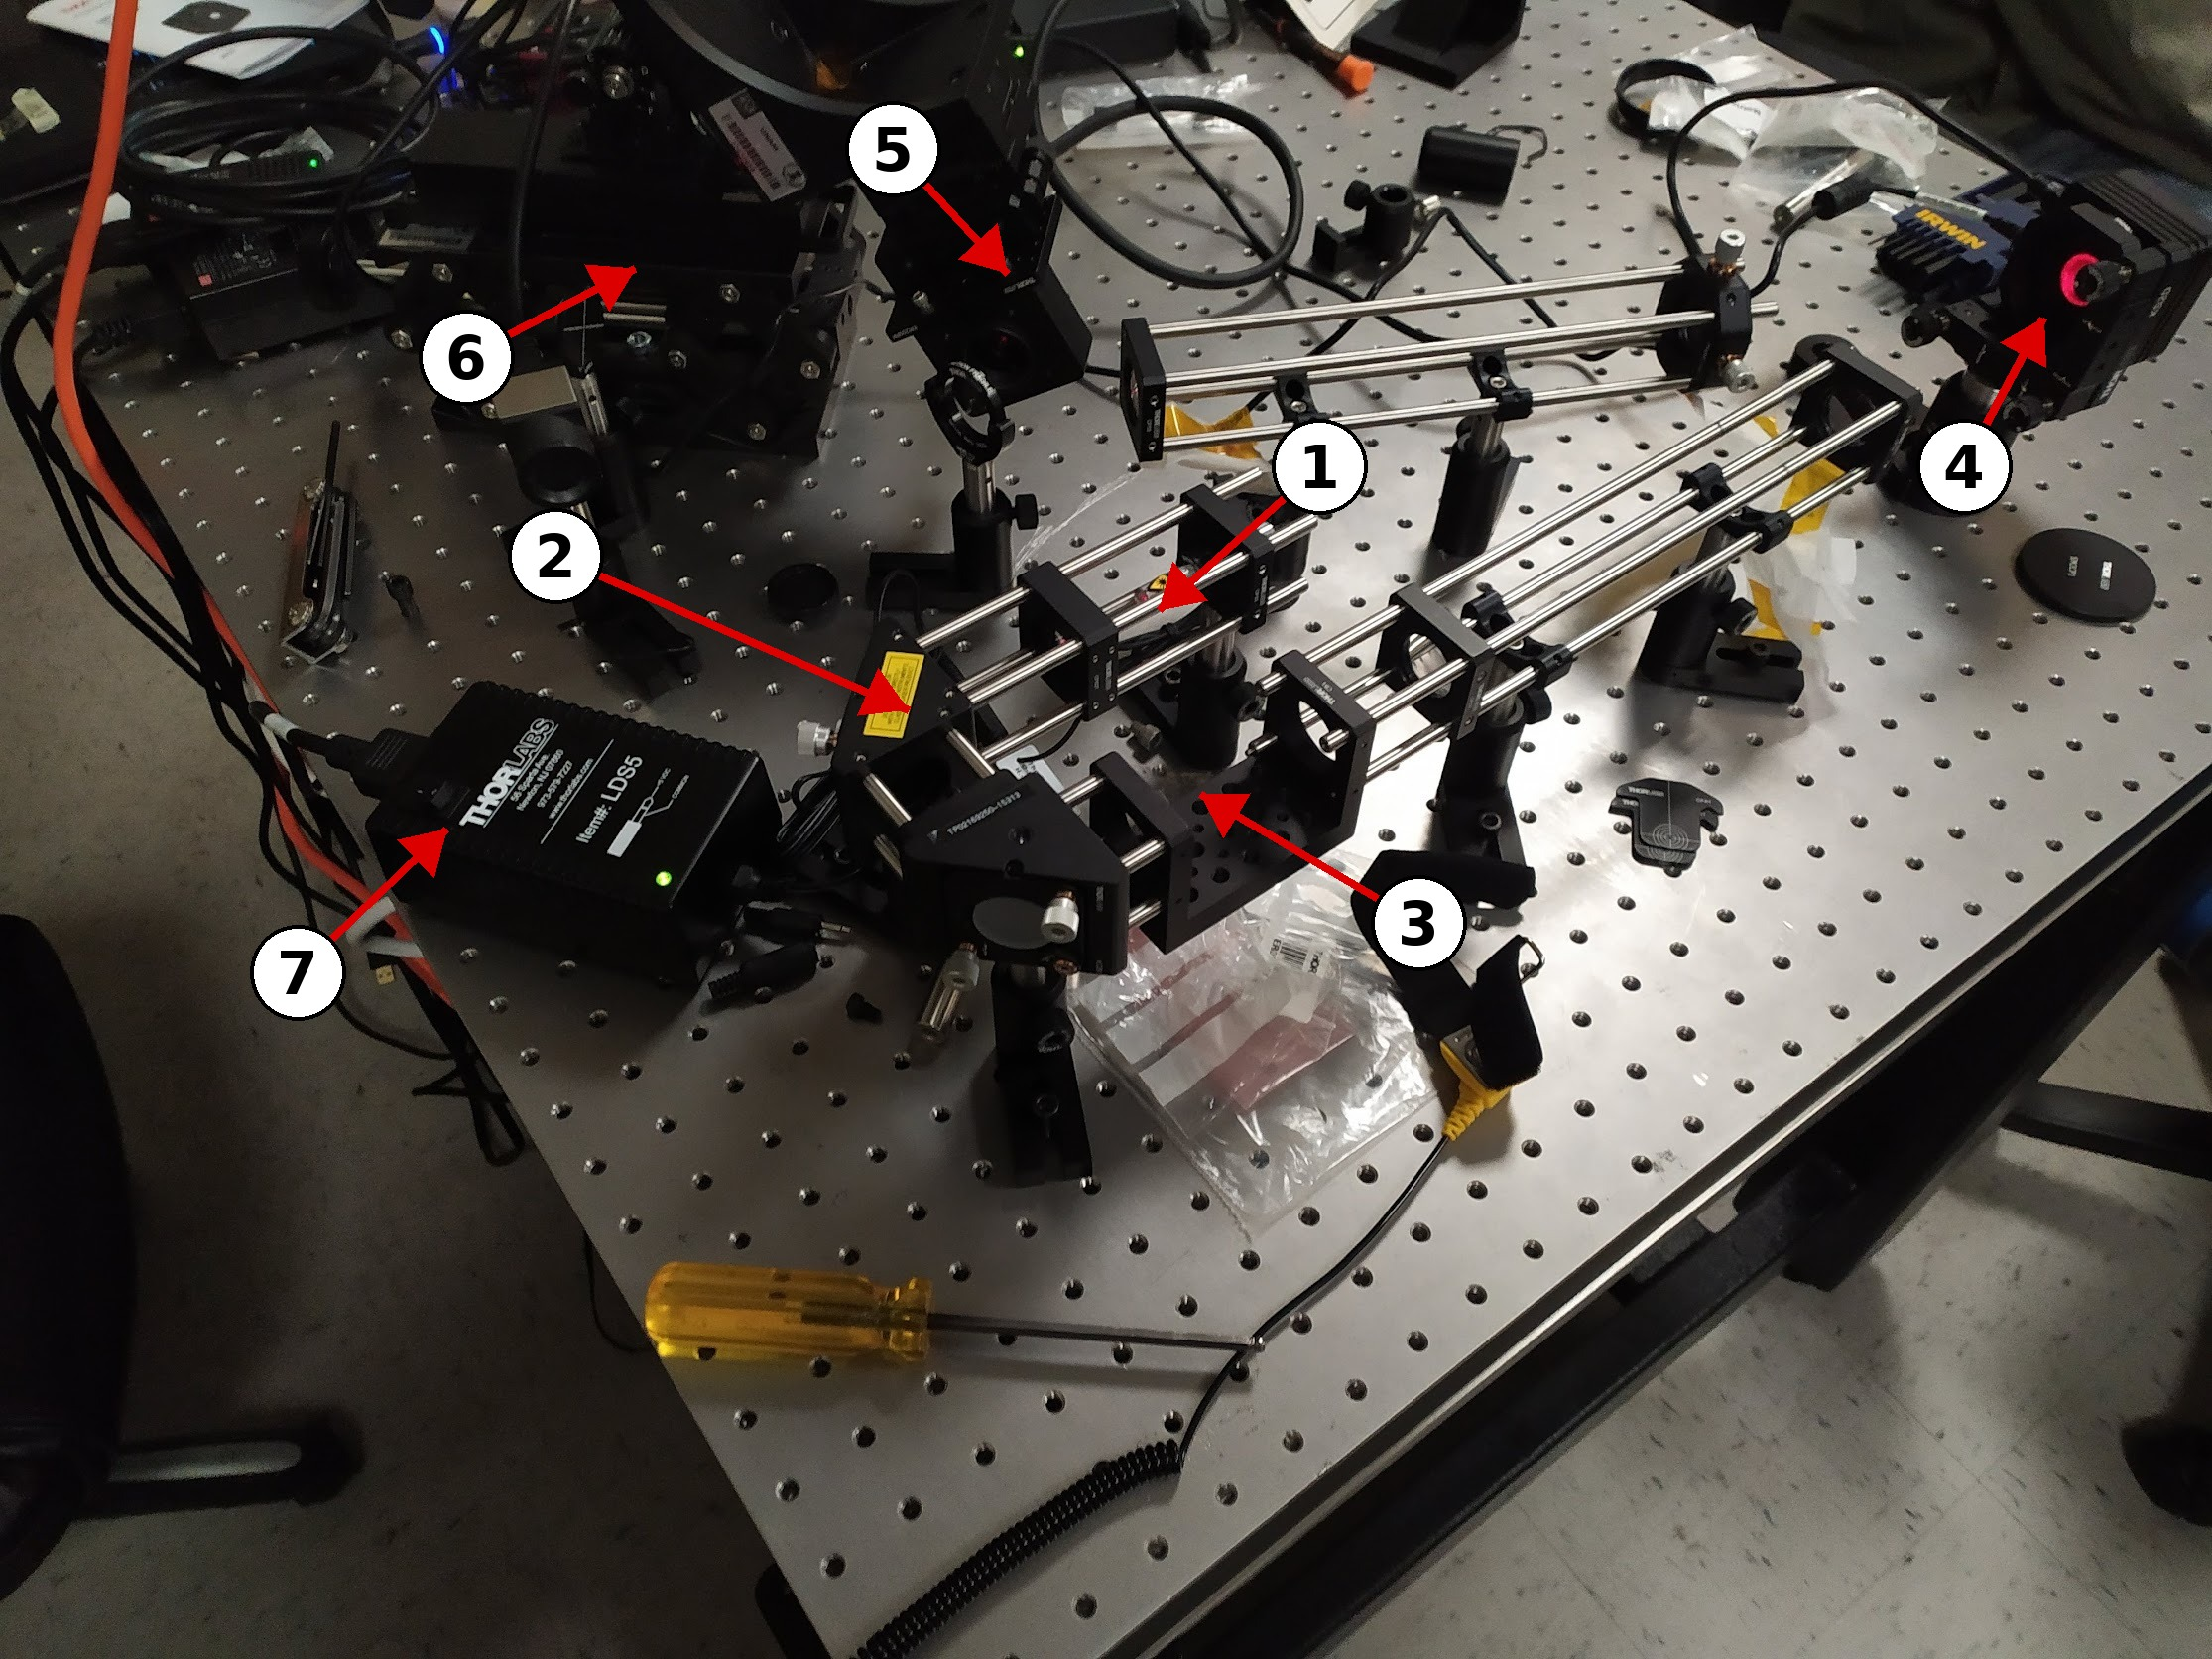
\includegraphics[width=\linewidth]{fotos/foto-montaje-completo-anotada.jpg}
	\caption{Vista general del montaje experimental sobre la mesa óptica. (1) Fuente de diodo
	láser (635 nm), apenas visible al inicio del camino; (2) espejos ajustables de la sección
	de expansión del kit AOK5/M; (3) plano de muestra, vacío en este trabajo; (4) espejo
	deformable DMP40-FM1 (el anillo rojo es el haz expandido desbordando su apertura); (5)
	sensor Shack-Hartmann WFS20-5C, parcialmente oculto tras su montura; (6) montura del
	sensor; (7) fuente de alimentación LDS5 del láser. El kit se emplea aquí únicamente para
	expandir y colimar el haz sobre el espejo deformable (Sección~\ref{sec:sistema-optico});
	no hay elemento bajo prueba en el plano de muestra. En esta toma el sensor descansa sobre
	un poste sencillo; el subsistema de posicionamiento con el que se realizaron los barridos
	se muestra en la Fig.~\ref{fig:foto-torre}.}
	\label{fig:foto-montaje}
\end{figure}

El sistema de posicionamiento realiza desplazamientos controlados del sensor siguiendo
patrones específicos determinados por los parámetros del método de corrimiento de puntos.
Para cada posición, el sensor Shack-Hart\-mann captura la información del frente de onda,
y los datos son almacenados por el sistema de adquisición para su posterior procesamiento.

La exactitud del sistema depende fundamentalmente de la alineación de cada componente
(Sección~\ref{sec:alineacion-sistema}) y de la secuencia manual de desplazamiento y
captura en cada posición del barrido (Sección~\ref{sec:adquisicion-datos}). A
continuación, se describen en detalle cada uno de estos subsistemas y sus características
técnicas.

\section{Sensor}

El sensor SH se compone de dos elementos principales. El primero es un sensor CMOS con una
resolución de 1440$\times$1080, un área sensible de 7.20$\times$5.40 mm y píxeles
cuadrados de 5$\mu m$, capaz de capturar hasta 1120 fps. El segundo elemento es un anillo
con un arreglo de microlentes planoconvexas de sílice fundida (MLA150-5C), el cual ha sido
previamente ajustado y calibrado por el fabricante, incluyendo un certificado de
calibración. Las microlentes son lentes esféricas de distancia focal 4.1 mm con 150$\mu m$
de separación entre estas, regular en ambas direcciones.

\begin{figure}[H]
	\centering
	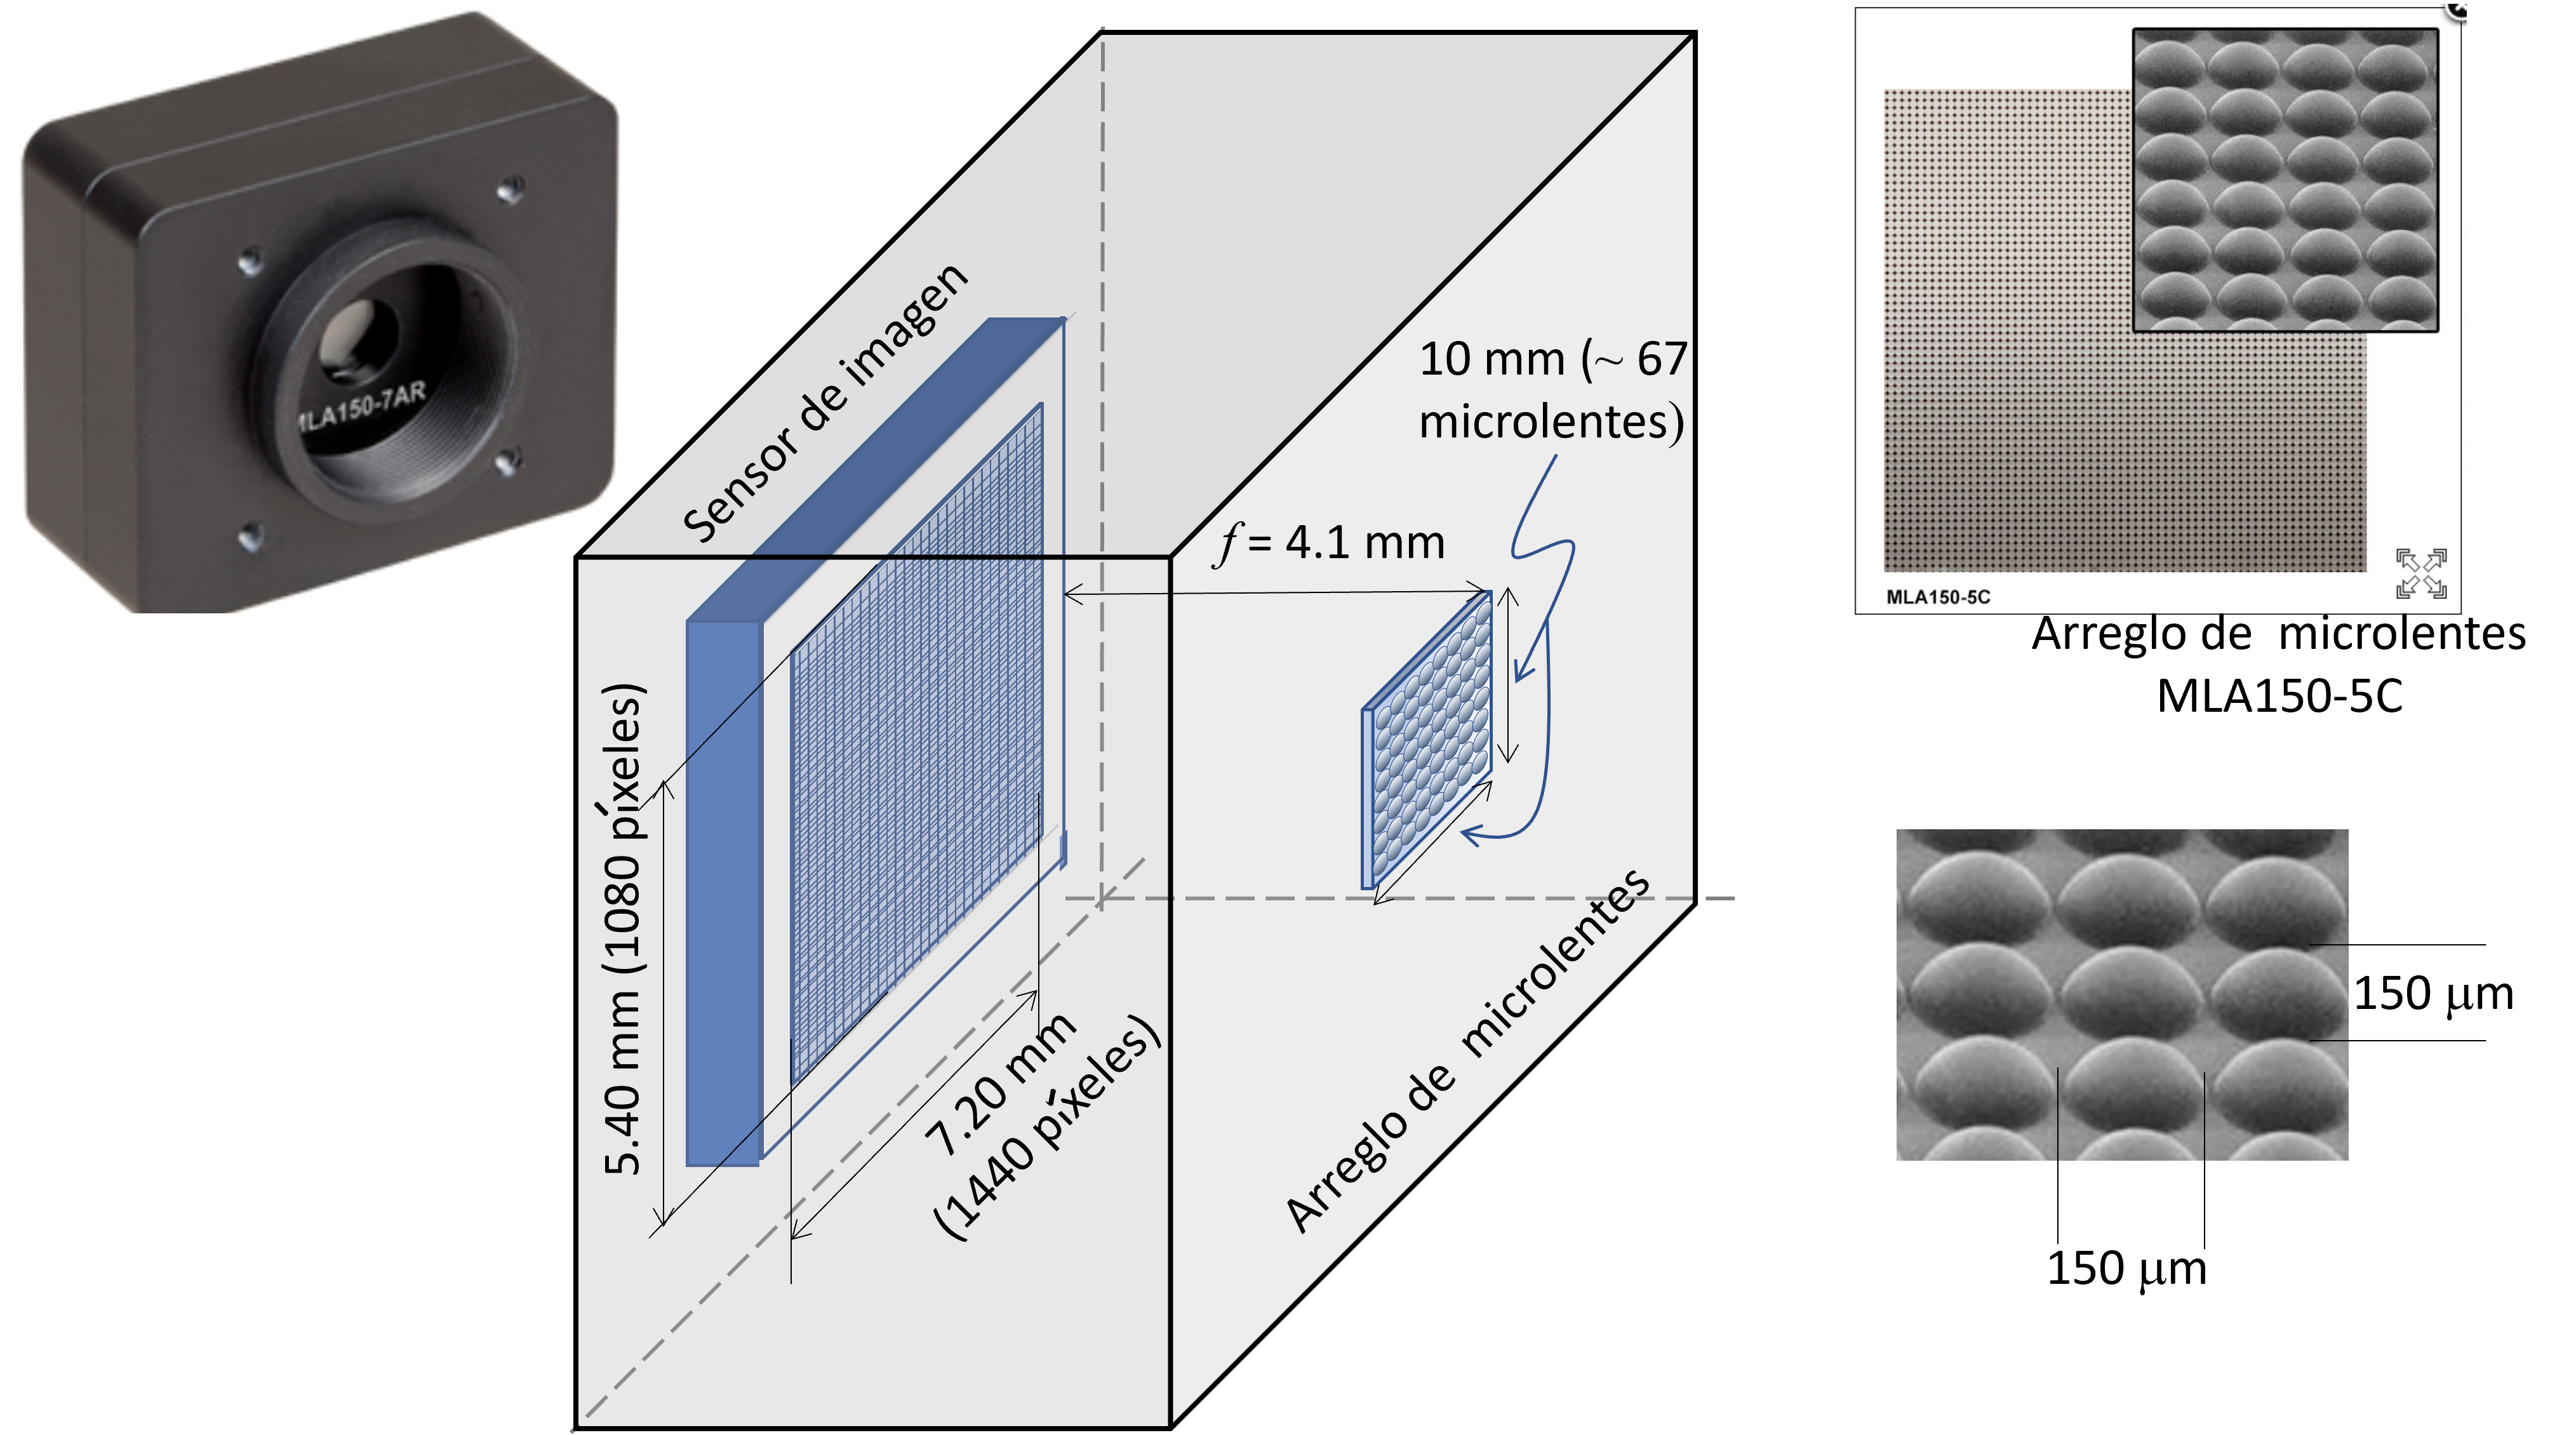
\includegraphics[width=0.85 \linewidth]{SH-Sensor-v2.png}
	\caption{Sensor Shack-Hartmann WFS20-5C (imagen tomada del catálogo del
	fabricante~\cite{ThorlabsCatalog}).}
	\label{fig:sh-sensor}
\end{figure}

Estos elementos conforman el sensor Shack-Hartmann (WFS20-5C) fabricado por Thorlabs, el
cual tiene una precisión de $\lambda/30$ RMS y una sensibilidad de hasta $\lambda/100$ RMS
utilizando su software.

\section{Sistema de posicionamiento y control}

\subsection{Ajuste de giro}

El sensor Shack-Hartmann WFS20-5C se entrega como una unidad cerrada con orificios de
montaje estándar, sin mecanismos propios para ajustar su inclinación, rotación o
desplazamiento fino. El método de corrimiento de puntos requiere, sin embargo, desplazar
el sensor con precisión micrométrica y rotarlo de forma controlada para acceder a las
distintas direcciones $(m,n)$ del muestreo. El subsistema de posicionamiento no fue
producto de un diseño previo, sino de una integración guiada por la necesidad: lo que
importaba era que el haz incidiera sobre el sensor, que el ángulo del sensor pudiera
fijarse con precisión suficiente y que los barridos de corrimiento fueran posibles; de ahí
la platina de desplazamiento motorizada y el goniómetro. Como el goniómetro limita el giro
a su recorrido, se añadió la platina de ángulo ajustable AP180 (pasos de $15^\circ$) para
alcanzar las direcciones $(m,n)$ requeridas; y como el apilamiento elevaba el sensor por
encima de la línea del haz, se agregaron la platina fija de $90^\circ$ y la mesa de altura
variable. Los componentes son los disponibles en el laboratorio (catálogos de Thorlabs y
Edmund Optics); con elementos de mayor rango o precisión el sistema de captura podría ser
más simple.

La montura del sensor se fijó a una platina de ajuste KM200PM con control de inclinación
en los dos ejes (\textit{tip} y \textit{tilt}) (ver Fig.~\ref{fig:KM200PM}). Esta platina
se acopló a su vez a un goniómetro Edmund Optics 66-526, que proporciona el ajuste fino
del ángulo: un recorrido de $\pm 10^\circ$ con resolución de 5 minutos de arco ($\approx
0.08^\circ$) según la ficha del fabricante~\cite{EdmundCatalog}, alineado al plano del
sensor como se muestra en la Fig.~\ref{fig:goniometroEdmun}.

\begin{figure}[htbp]
	\centering
	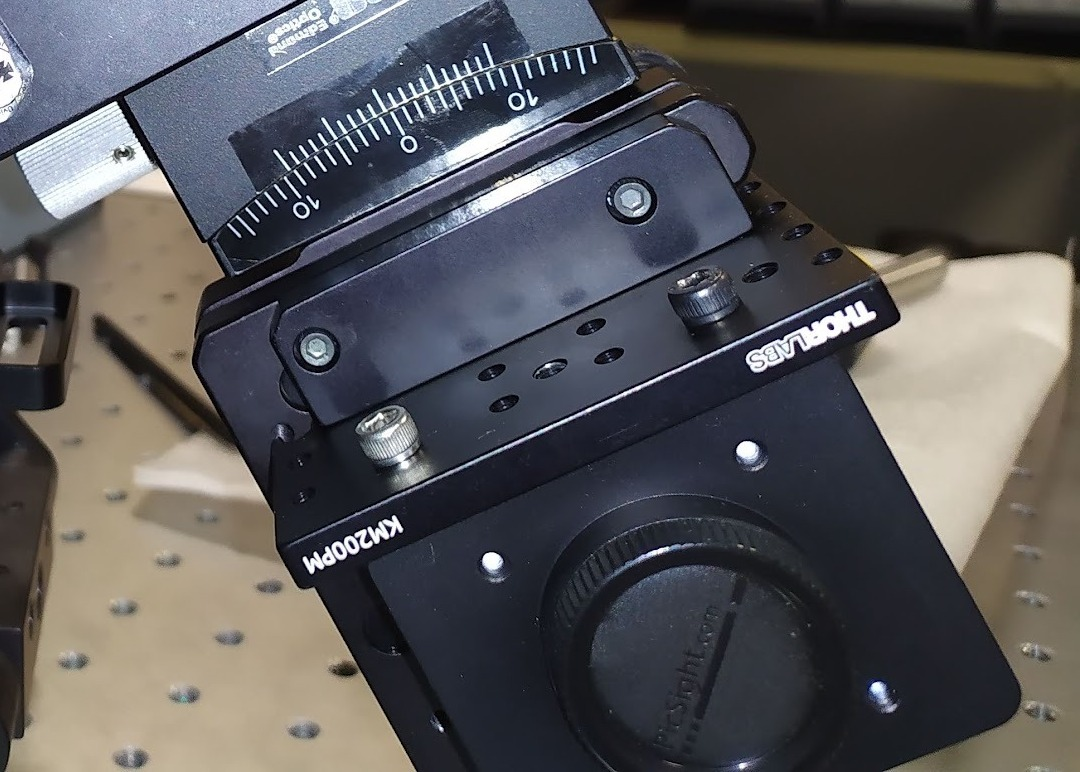
\includegraphics[width=0.45 \textwidth]{fotos/foto-km200pm-recorte.jpg}
	\caption{Montura de ajuste \textit{tip-tilt} KM200PM que sujeta al sensor (detalle del
	montaje; el conjunto está invertido, por lo que la etiqueta se lee al revés). Arriba se
	aprecia la escala del goniómetro.}
	\label{fig:KM200PM}
\end{figure}

\begin{figure}[htbp]
	\centering
	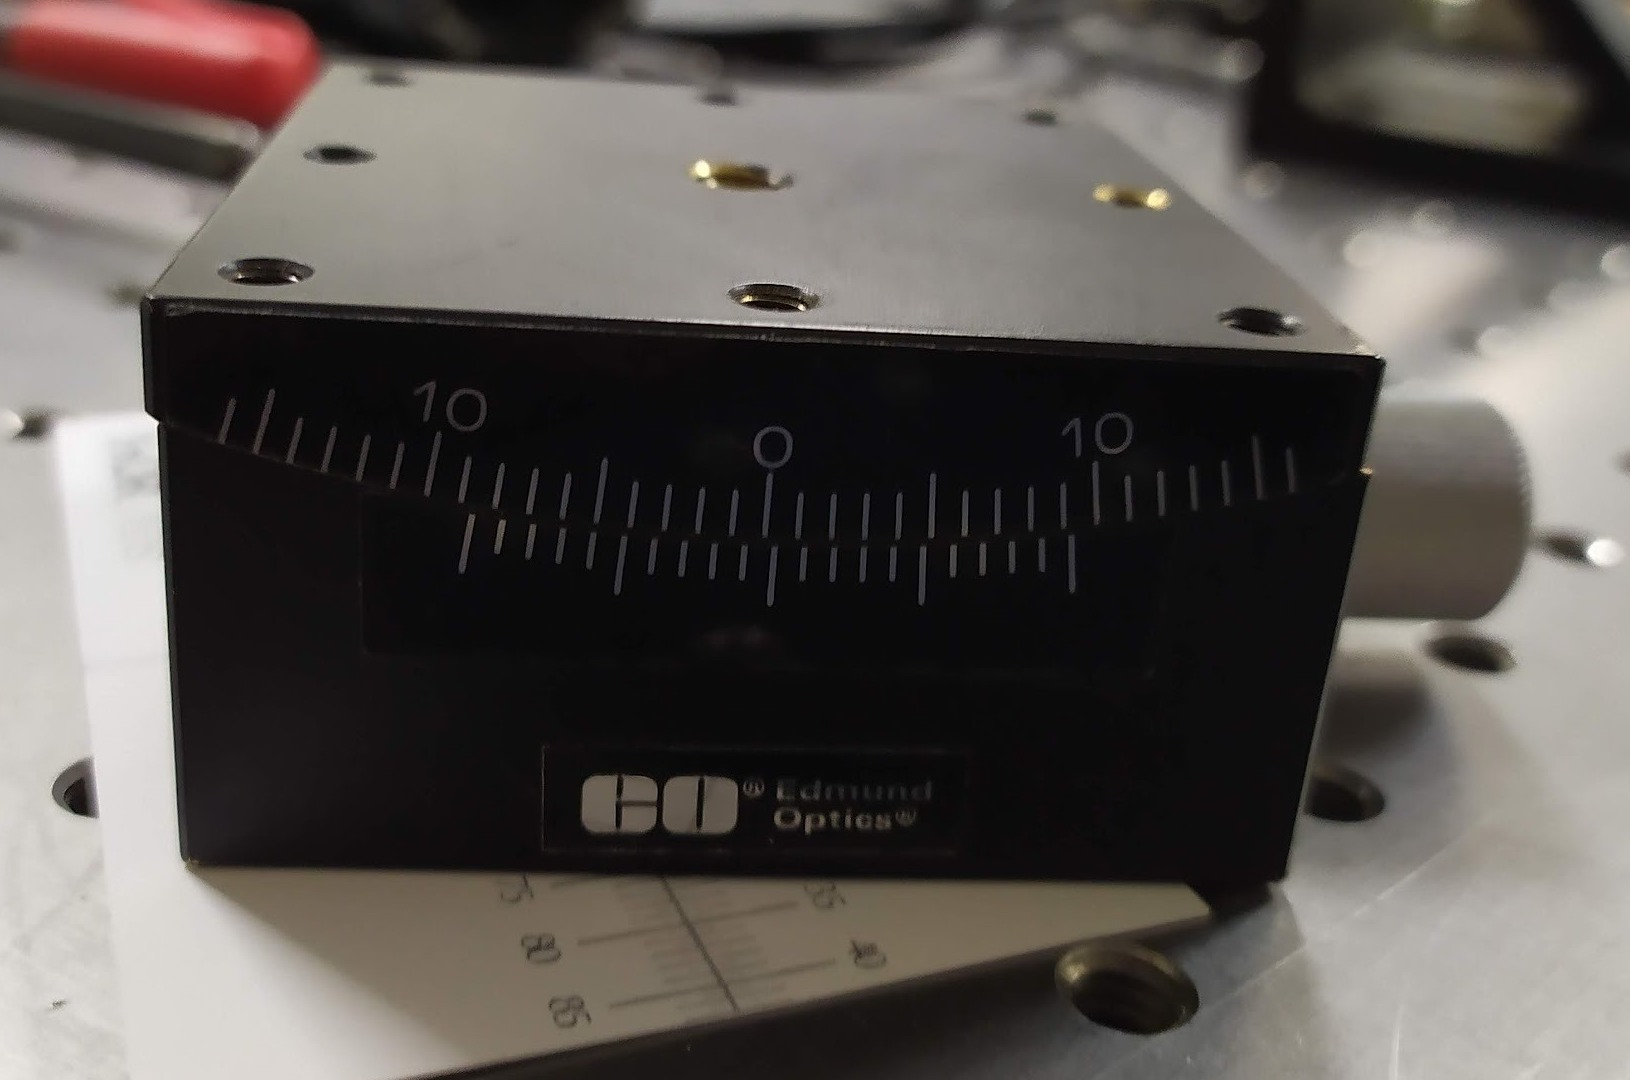
\includegraphics[width=0.5 \textwidth]{fotos/foto-goniometro-recorte.jpg}
	\caption{Goniómetro Edmund Optics 66-526 empleado para el ajuste fino del ángulo del
	sensor. Se aprecia la escala de $\pm 10^\circ$ y el nonio con el que se lee la resolución
	de 5 minutos de arco~\cite{EdmundCatalog}.}
	\label{fig:goniometroEdmun}
\end{figure}

El goniómetro se montó sobre una platina de ángulo ajustable Thorlabs AP180, que
proporciona el ajuste grueso: trece posiciones discretas cada $15^\circ$ a lo largo de
$180^\circ$, fijadas con un pasador, con una precisión de $\pm 18'$ ($\approx \pm
0.3^\circ$) según el fabricante~\cite{ThorlabsCatalog} (ver Fig.~\ref{fig:APT180}). Los
dos elementos trabajan en conjunto: la AP180 lleva el sensor al múltiplo de $15^\circ$ más
cercano al ángulo de barrido requerido y el goniómetro corrige la diferencia, que por
construcción nunca supera $7.5^\circ$ y cabe dentro de su recorrido. Así el ángulo de
barrido se fija con la resolución del goniómetro sobre todo el rango de la AP180.

\begin{figure}[htbp]
	\centering
	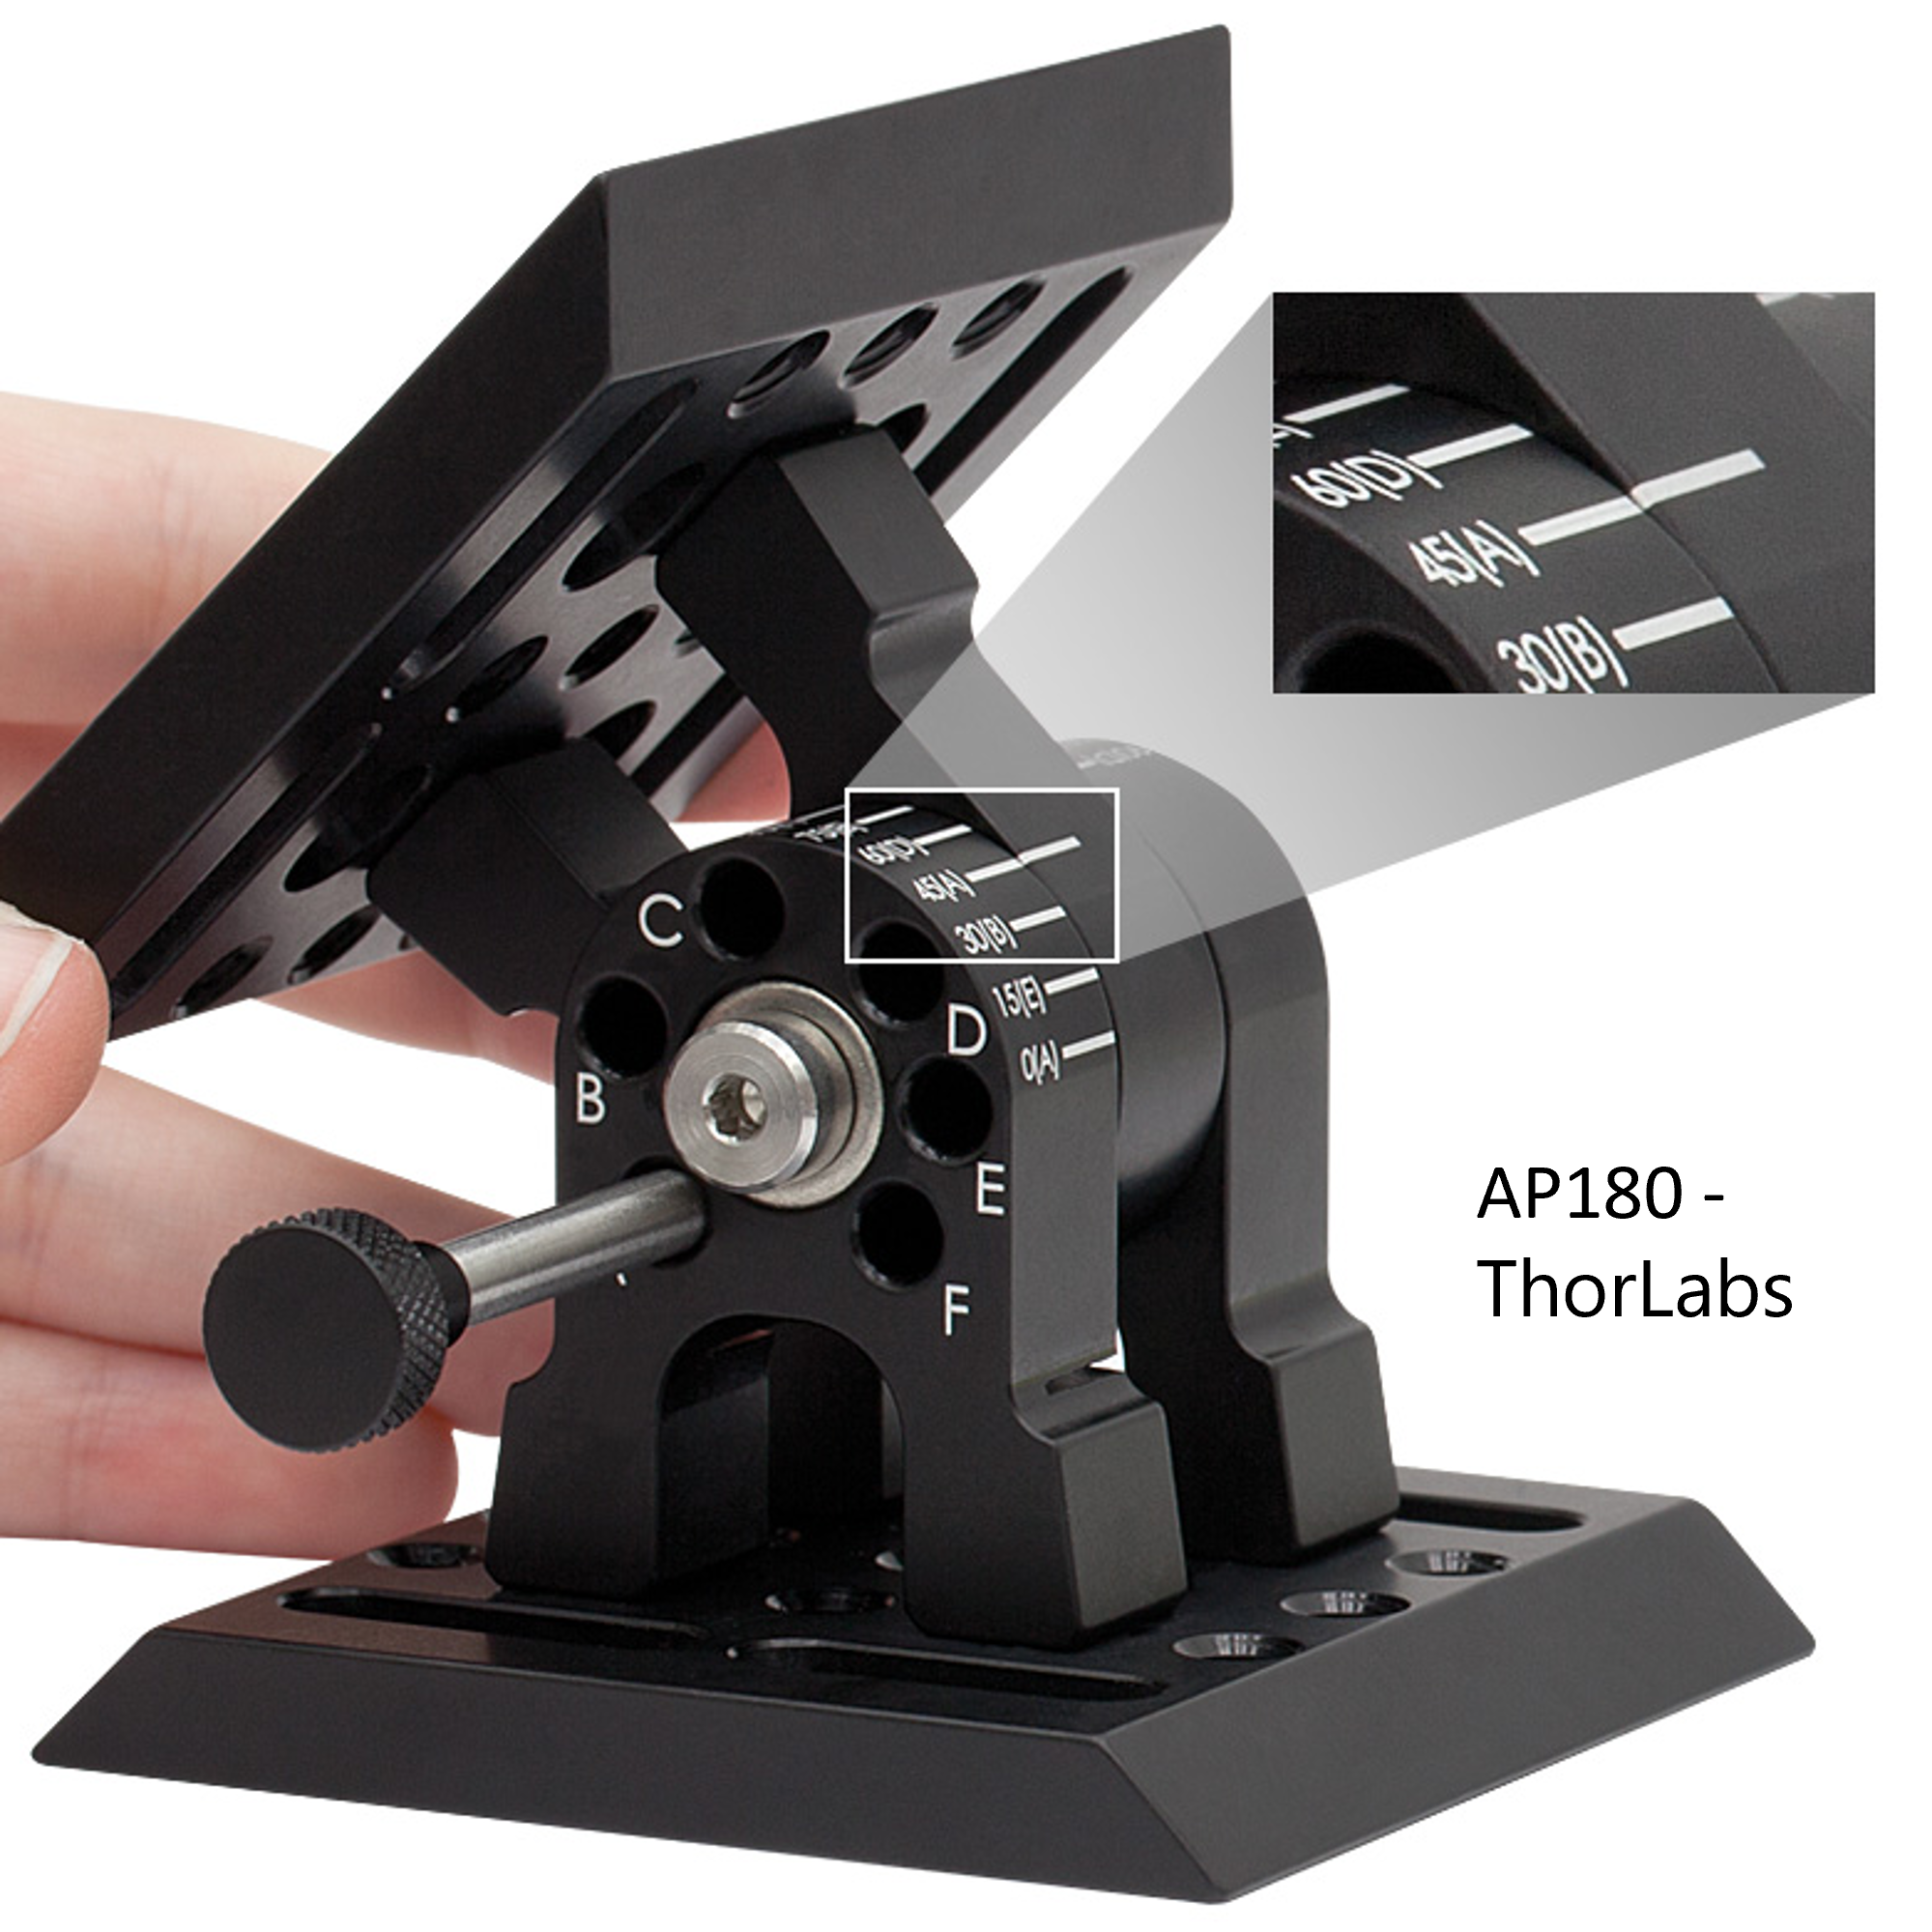
\includegraphics[width=0.3 \textwidth]{APT180.png}
	\caption{Platina de rotación de ángulo ajustable AP180 (imagen tomada del catálogo del
	fabricante~\cite{ThorlabsCatalog}).}
	\label{fig:APT180}
\end{figure}

Entre el goniómetro y la AP180 se intercaló una platina fija de $90^\circ$. Su función es
práctica: apilados, el goniómetro y la AP180 dejaban el sensor muy por encima de la línea
del haz; con la AP180 fijada a $90^\circ$ hacia abajo, la placa de $90^\circ$ invierte el
conjunto completo y el sensor queda colgando a la altura del haz (ver
Fig.~\ref{fig:sistema-angular} y las fotografías de la Fig.~\ref{fig:foto-torre}). Esa
posición invertida, con el goniómetro en cero, es la referencia desde la que se miden
todos los ángulos de barrido (Sección~\ref{sec:ajuste-angulo}). La inversión no afecta a
la medición: lo que importa es la dirección de desplazamiento en el plano del sensor, que
es la misma recta con el conjunto invertido o no, y la distancia entre posiciones
consecutivas; el sentido se registra siempre respecto a la platina de desplazamiento, sin
ninguna corrección de signo. Como cada cambio de ángulo modifica la altura efectiva del
sensor (el centro de giro no coincide con el plano de detección), el conjunto descansa
sobre una mesa de altura variable Thorlabs L490 que permite devolver el sensor al plano
del haz tras cada ajuste (ver Fig.~\ref{fig:mesaVariable}).

\begin{figure}[H]
	\centering
	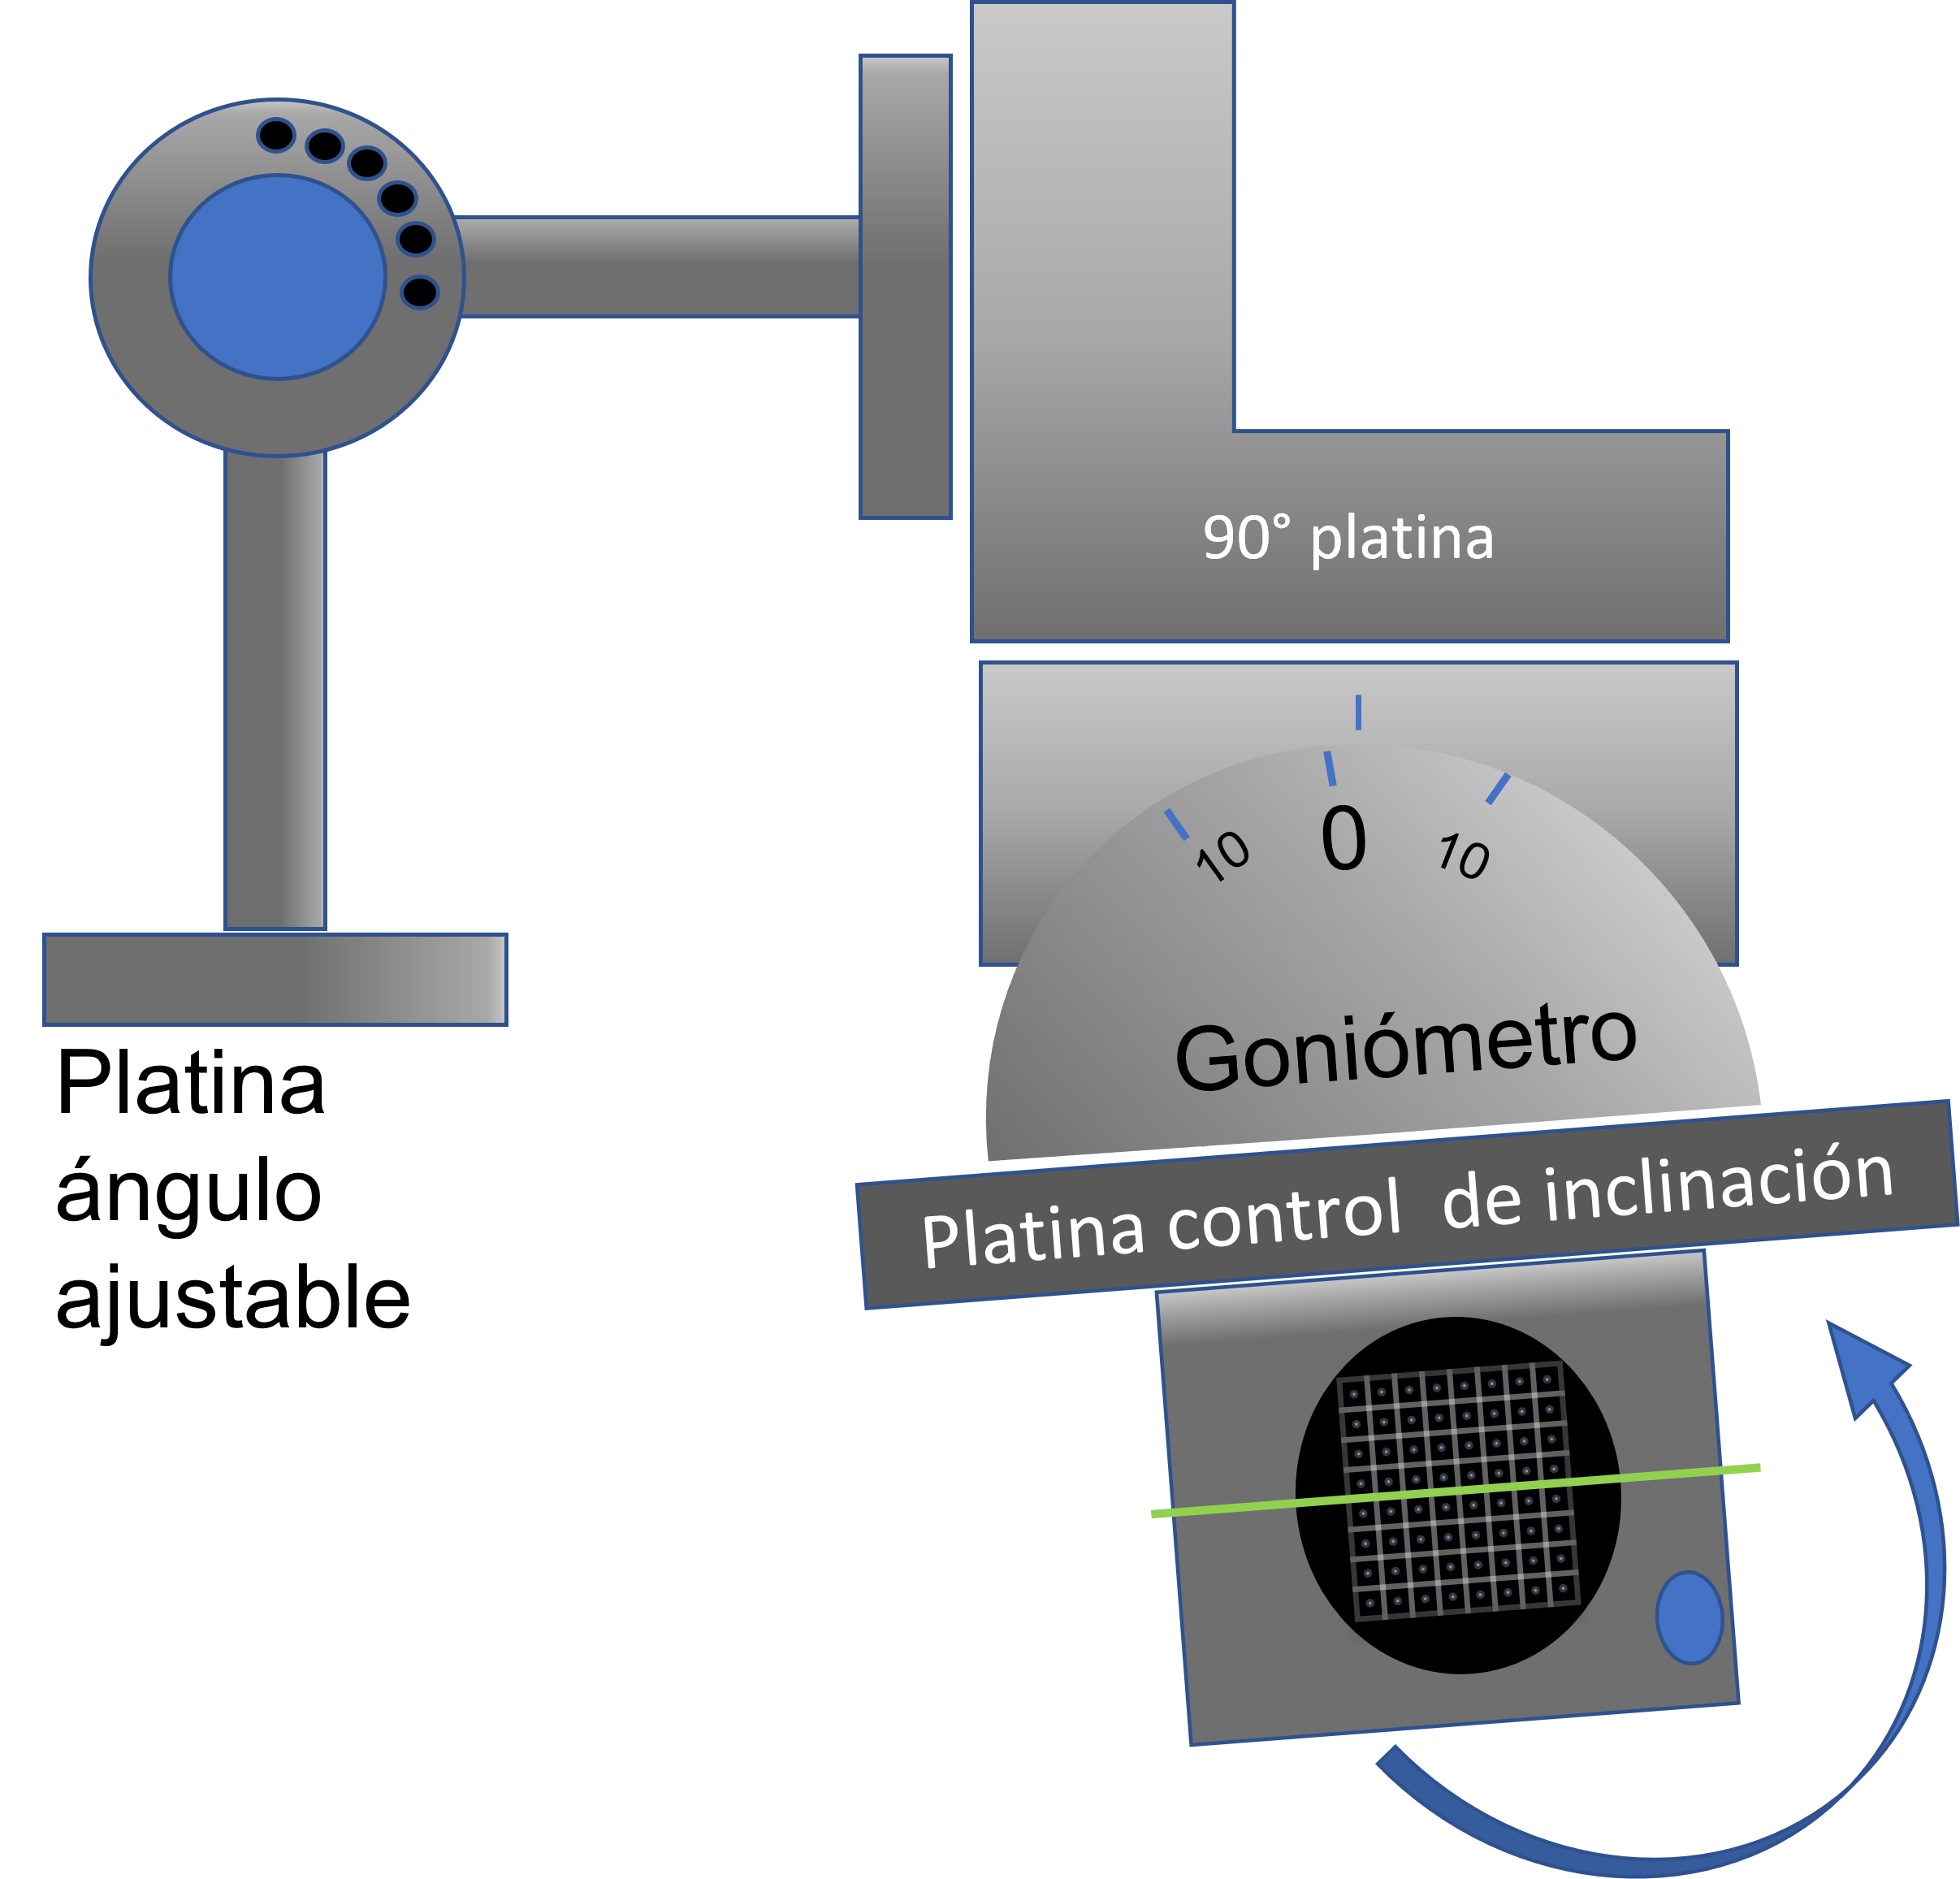
\includegraphics[width=0.4\linewidth]{Sistema ángular-v2.png}
	\caption{Diagrama del control y sistema angular}
	\label{fig:sistema-angular}
\end{figure}

\begin{figure}[htbp]
	\centering
	\begin{minipage}[t]{0.49\linewidth}
		\centering
		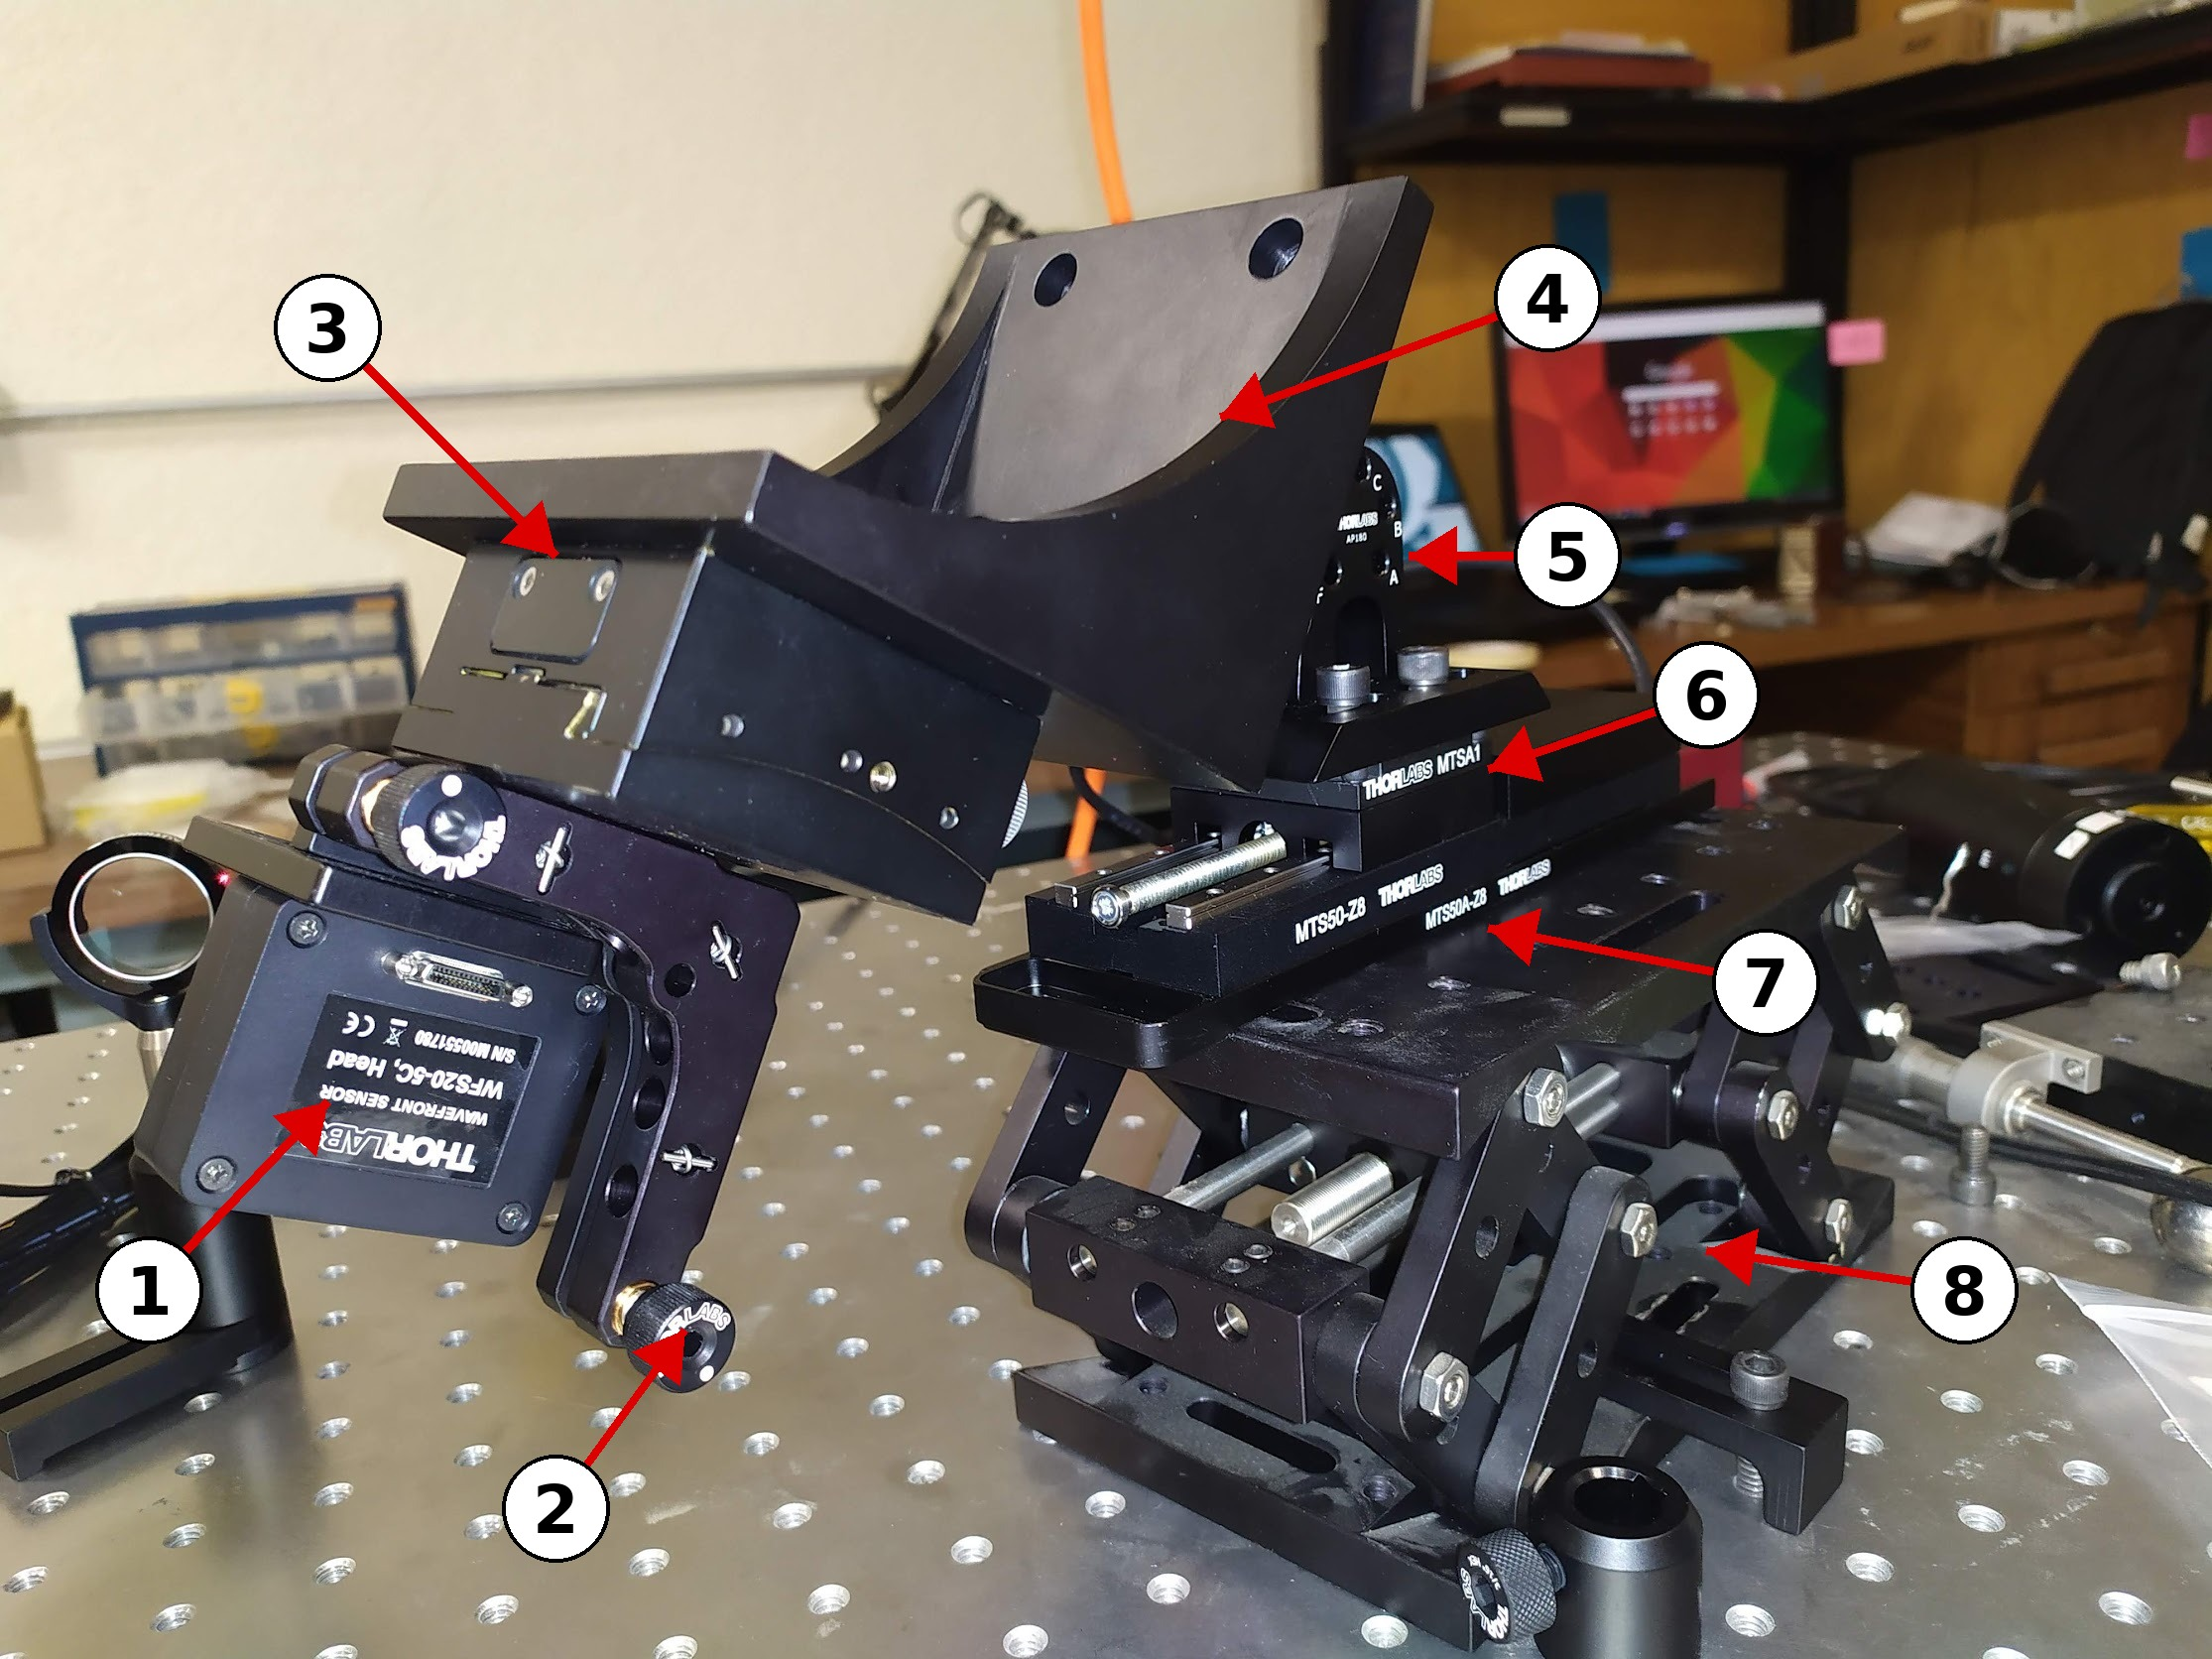
\includegraphics[width=\linewidth]{fotos/foto-torre-final-anotada.jpg}\\[2pt]
		\textbf{(a)}
	\end{minipage}\hfill
	\begin{minipage}[t]{0.49\linewidth}
		\centering
		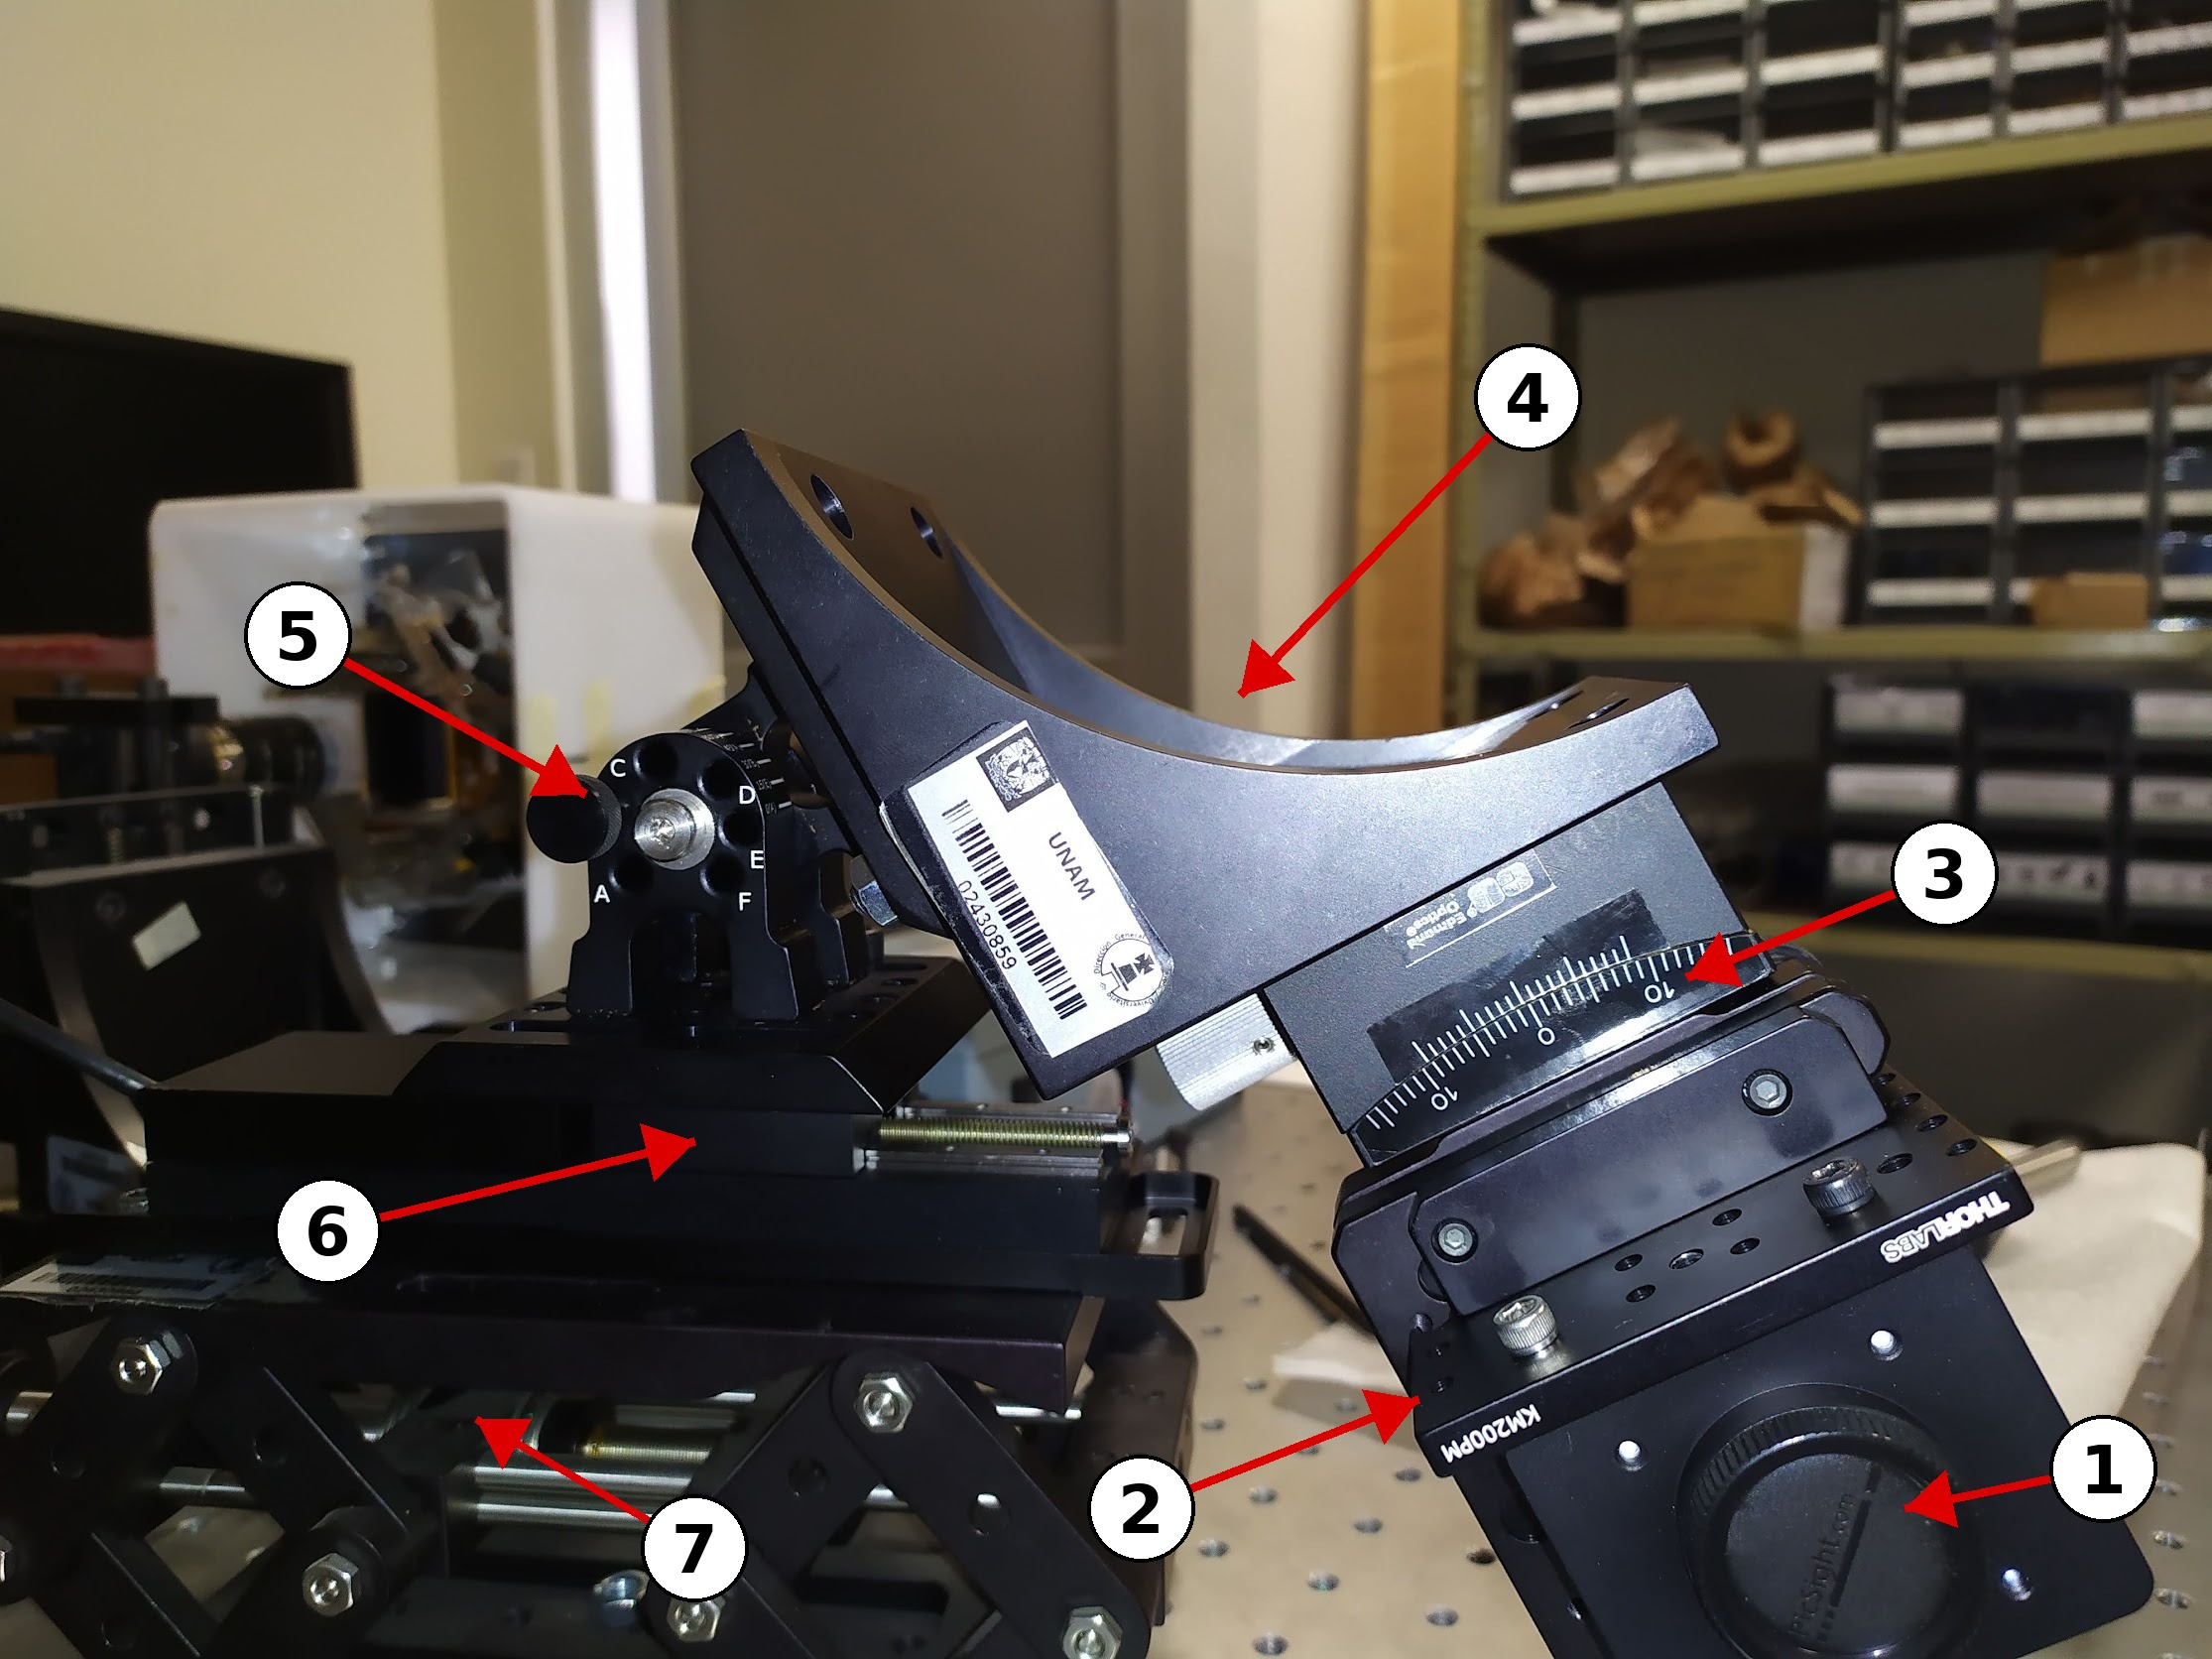
\includegraphics[width=\linewidth]{fotos/foto-torre-detalle-anotada.jpg}\\[2pt]
		\textbf{(b)}
	\end{minipage}
	\caption{Subsistema de posicionamiento del sensor. \textbf{(a)} Configuración completa:
	(1) sensor WFS20-5C, montado invertido; (2) montura de inclinación \textit{tip-tilt}; (3)
	goniómetro Edmund Optics 66-526, visto por detrás; (4) placa fija de $90^\circ$; (5)
	platina de ángulo ajustable AP180, con pasador cada $15^\circ$; (6) placa adaptadora
	MTSA1; (7) platina motorizada MTS50-Z8, que ejecuta los corrimientos; (8) mesa de altura
	variable L490. \textbf{(b)} El mismo conjunto visto desde el lado opuesto: (1) sensor;
	(2) montura de inclinación; (3) escala del goniómetro, $10\cdot 0\cdot 10$ ($\pm
	10^\circ$); (4) placa de $90^\circ$; (5) AP180, con el pasador en una de las posiciones
	A--F; (6) platina MTS50-Z8; (7) mesa L490. La dirección de barrido se fija con la AP180 y
	el goniómetro antes de medir; durante el barrido sólo se mueve la platina motorizada.}
	\label{fig:foto-torre}
\end{figure}

\subsection{Control de desplazamiento y altura}\label{sec:control-desplazamiento-altura}

\begin{figure}[htbp]
	\centering
	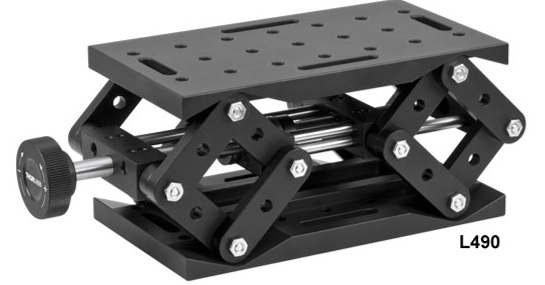
\includegraphics[width=0.35 \textwidth]{mesaVaraible.png}
	\caption{Mesa de altura variable L490 (imagen tomada del catálogo del
	fabricante~\cite{ThorlabsCatalog}).}
	\label{fig:mesaVariable}
\end{figure}

El sistema de control angular descrito anteriormente fue colocado sobre una platina de
desplazamiento motorizada por pasos (MTS50-Z8, Fig.~\ref{fig:platinadesplazamiento}), que
permite un desplazamiento en una dimensión vertical, con un rango de movimiento de 50 mm,
un movimiento mínimo alcanzable de 0.05 $\mu$m, un incremento mínimo repetible de 0.8
$\mu$m y una repetibilidad bidireccional de 1.6 $\mu$m. La platina soporta una carga
horizontal recomendada menor a 10 kg con un máximo de 12 kg. Para controlar su movimiento
se emplea un controlador de servomotor KDC101 (ver Fig.~\ref{fig:Motor}), cuyo software
dedicado permite configurar con precisión la distancia de cada paso de acuerdo con los
parámetros calculados para el método de corrimiento de puntos.

\begin{figure}[htbp]
	\centering
	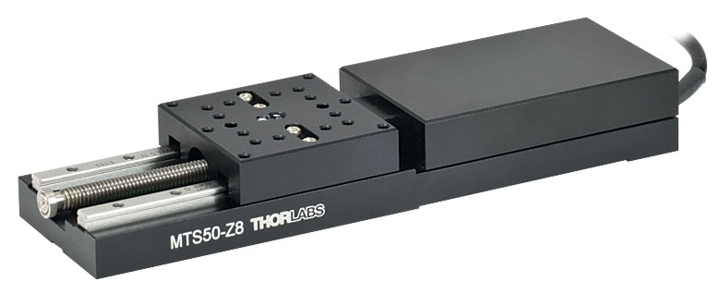
\includegraphics[width=0.8\linewidth]{platinaDesplazamiento.png}
	\caption{Platina de desplazamiento motorizada MTS50-Z8 (imagen tomada del catálogo del
	fabricante~\cite{ThorlabsCatalog}).}
	\label{fig:platinadesplazamiento}
\end{figure}

Finalmente, la platina descansa sobre una mesa de altura variable que permite el reajuste
de altura, como se muestra en la Fig.~\ref{fig:sistema-optico}. Debido al movimiento en
altura generado por el goniómetro y la platina de giro de 15°, la altura del sensor varía
considerablemente, lo que puede causar que el sensor salga del plano de propagación del
haz bajo prueba.

\begin{figure}[htbp]
	\centering
	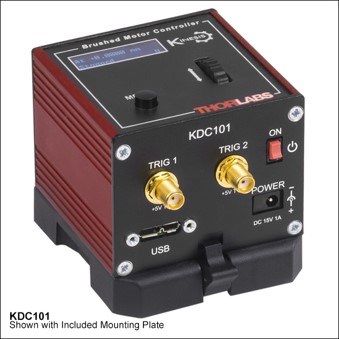
\includegraphics[width=0.3 \textwidth]{Motor.jpg}
	\caption{Controlador de servomotor KDC101 (imagen tomada del catálogo del
	fabricante~\cite{ThorlabsCatalog}).}
	\label{fig:Motor}
\end{figure}

Para alimentar el controlador KDC101 y el sistema de óptica adaptativa descrito en la
sección siguiente se emplea una fuente de alimentación estabilizada PPT2415, que
suministra el voltaje requerido por ambos componentes.

\section{Sistema óptico}\label{sec:sistema-optico}

Este trabajo emplea el kit Sistema de Óptica Adaptativa Ensamblado (AOK5/M) proporcionado
por Thorlabs, una elección basada en las capacidades avanzadas del kit. En particular, el
sistema permite la generación de frentes de onda con deformaciones controlables y
repetibles a través de los actuadores del espejo deformable, lo que resulta crucial para
producir frentes de onda con modos de Zernike de orden alto de manera consistente y poder
así someter al método de corrimiento de puntos a aberraciones fuertes en condiciones
reproducibles.

\begin{figure}[htbp]
	\centering 
	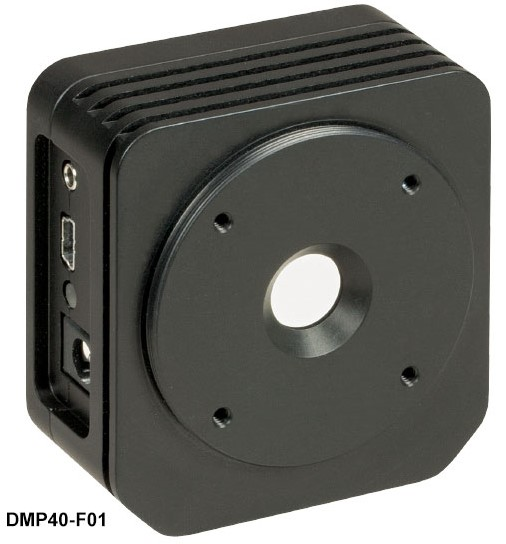
\includegraphics[width=0.3 \textwidth]{EspejoDeformable.jpg}
	\caption{Espejo deformable DMP40-FM1 (imagen tomada del catálogo del
	fabricante~\cite{ThorlabsCatalog}).}
	\label{fig:espejo-deformable-MP}
\end{figure}

El kit AOK5(/M) se ofrece originalmente con un Multi-DM (DM140A-35-P01, 140 actuadores
MEMS); en este trabajo dicho espejo fue sustituido por un DMP40-FM1, un espejo deformable
piezoeléctrico de 40 actuadores que ofrece mayor amplitud de deformación; la histéresis
propia de los actuadores piezoeléctricos se maneja mediante la compensación por software
del controlador del fabricante. Esta sustitución es favorable para el método de
corrimiento de puntos, ya que permite imponer aberraciones de gran amplitud con órdenes
Zernike altos de manera reproducible. El manual del kit contempla esta configuración y
especifica una distancia de alineación de aproximadamente 73 mm para el DMP40.

El espejo deformable, conocido por su modelo DMP40-FM1, está compuesto por una superficie
reflejante que puede ser flexionada y adaptada gracias a sus 40 actuadores distribuidos en
una configuración circular. Esto permite no solo reflejar la luz, sino también modificar
activamente el frente de onda de la luz reflejada. Una característica destacada de este
espejo es su conectividad USB, permitiendo a una computadora enviar comandos y ajustar la
forma del espejo deformable en tiempo real. Mediante el software proporcionado por
Thorlabs, es posible tener un control preciso sobre la deformación del espejo, permitiendo
ajustar individualmente cada actuador o seguir formas predefinidas (modos de Zernike), con
control de los términos $Z_4$ a $Z_{15}$ en la convención que se detalla en la
Sección~\ref{sec:convencion-zernike}.

En este trabajo, el espejo deformable es la fuente de los frentes de onda bajo prueba. Un
haz colimado con frente de onda plano incide sobre él y, al deformarse su superficie según
la configuración de sus actuadores, el espejo modifica la fase del frente de onda
reflejado; el resto del sistema de óptica adaptativa sólo expande y colima el haz sobre el
espejo. Visto desde el sensor, el conjunto equivale a una fuente de luz cuyo frente de
onda tiene una fase ajustable, y ésa es la única función que cumple aquí. \emph{Ajustable}
no significa \emph{conocida}: lo que se fija y se conoce es la configuración del espejo
—el modo de Zernike activado en el software de control y la amplitud de su deslizador
(Sección~\ref{sec:convencion-zernike})—, no el frente de onda resultante, que no se
caracteriza de forma independiente en esta tesis; por qué esto basta para validar el
método se discute en la Sección~\ref{sec:comparacion}. El objeto de evaluación es, por
tanto, el frente de onda que el espejo produce y no la superficie del espejo: en reflexión
próxima a la normal, la aberración del frente de onda es el doble de la deformación local
de la superficie~\cite{BribiescasTesis}. Que el espejo pueda generar aberraciones de gran
amplitud es, además, una decisión de diseño del experimento: permite poner a prueba el
método en condiciones exigentes, y por ello las evaluaciones del
Capítulo~\ref{cap:resultados} usan los modos $Z_{11}$ y $Z_{13}$ cerca de su amplitud
negativa máxima.

Dentro del kit, las secciones vienen prealineadas de fábrica. Estas secciones, diseñadas
para funcionar en conjunto, forman el sistema de óptica adaptativa:

\begin{enumerate}
	\item La primera sección del kit AOK5(/M) es la encargada de la generación y expansión del haz de luz. Incluye una fuente de diodo láser que emite luz de 635 nm de longitud de onda, con una potencia aproximada de 0.3 mW. Esta luz pasa inicialmente por una lente LA1131-B de 50 mm de longitud focal, que forma un foco intermedio del haz láser sobre el plano de muestra alojado dentro de la caja CBB1 (vacío en este trabajo). El haz divergente desde ese foco es reflejado y redireccionado por dos espejos PF10-03-P01 con recubrimiento de plata protegida, de alta reflectancia en un rango amplio de longitudes de onda, y finalmente una lente LA1608-B de 75 mm de longitud focal recolima el haz expandido (de aproximadamente 2 cm de diámetro) para que sobrepase la apertura del espejo deformable.
	
	\item La segunda sección es un relevo de dos lentes LA1608-B de 75 mm de distancia focal que conduce el haz expandido y colimado hasta el espejo deformable; en el diseño del kit, el haz a su salida tiene unos 2 cm de diámetro y cubre por completo la apertura del espejo~\cite{ThorlabsAOKManual}.
	
	\item La tercera sección, el brazo de retorno, recoge el haz reflejado por el espejo deformable con otras dos lentes de 75 mm de distancia focal y lo lleva al divisor de haz y al sensor. En el diseño del kit este relevo forma la imagen del espejo sobre el arreglo de microlentes cuando la distancia de la última lente al arreglo, pasando por el divisor, es de unos 75 mm~\cite{ThorlabsAOKManual}.
\end{enumerate}

Las posiciones del espejo deformable y del brazo de retorno se fijaron con las distancias
y el ángulo nominales que el manual del kit indica para el DMP40: unos 73 mm entre la
última lente de la segunda sección y la superficie del espejo, y $35^\circ$ entre el haz
incidente y el brazo de retorno~\cite{ThorlabsAOKManual}. El ángulo se trazó por
trigonometría sobre la mesa y la trayectoria reflejada se alineó con un puntero láser y un
espejo plano colocado provisionalmente en la posición del espejo deformable, usando las
propias monturas del kit como referencia. El brazo de retorno se montó girado hacia el
lado opuesto al del manual, imagen especular del arreglo original, lo que no altera
distancias ni ángulos y sólo invierte lateralmente la imagen del espejo sobre el sensor,
algo irrelevante para una comparación entre reconstrucciones del mismo frente de onda. Al
montar el subsistema de posicionamiento del sensor se procuró conservar la distancia
nominal de la última lente al sensor, pero no se midió ni se ajustó con ese fin: la
conjugación entre el espejo y el arreglo de microlentes es la del diseño del kit y no se
verificó en este trabajo. Tampoco se midió la colimación del haz por separado: las
secciones del kit se emplearon prealineadas de fábrica. Ninguna de las dos cosas afecta a
la validación del método, que compara dos reconstrucciones del mismo frente de onda a
partir de los mismos centroides (Sección~\ref{sec:comparacion}).

Una vez que la luz ha pasado por estas secciones, un divisor de haz de película delgada
BP108 8:92 (R:T) refleja una fracción de la luz hacia el sensor Shack-Hartmann, como en el
arreglo del manual; la fracción transmitida se bloquea o puede redirigirse a otra
aplicación. La Fig.~\ref{fig:foto-divisor} muestra este tramo final del sistema óptico en
el montaje real.

\begin{figure}[htbp]
	\centering
	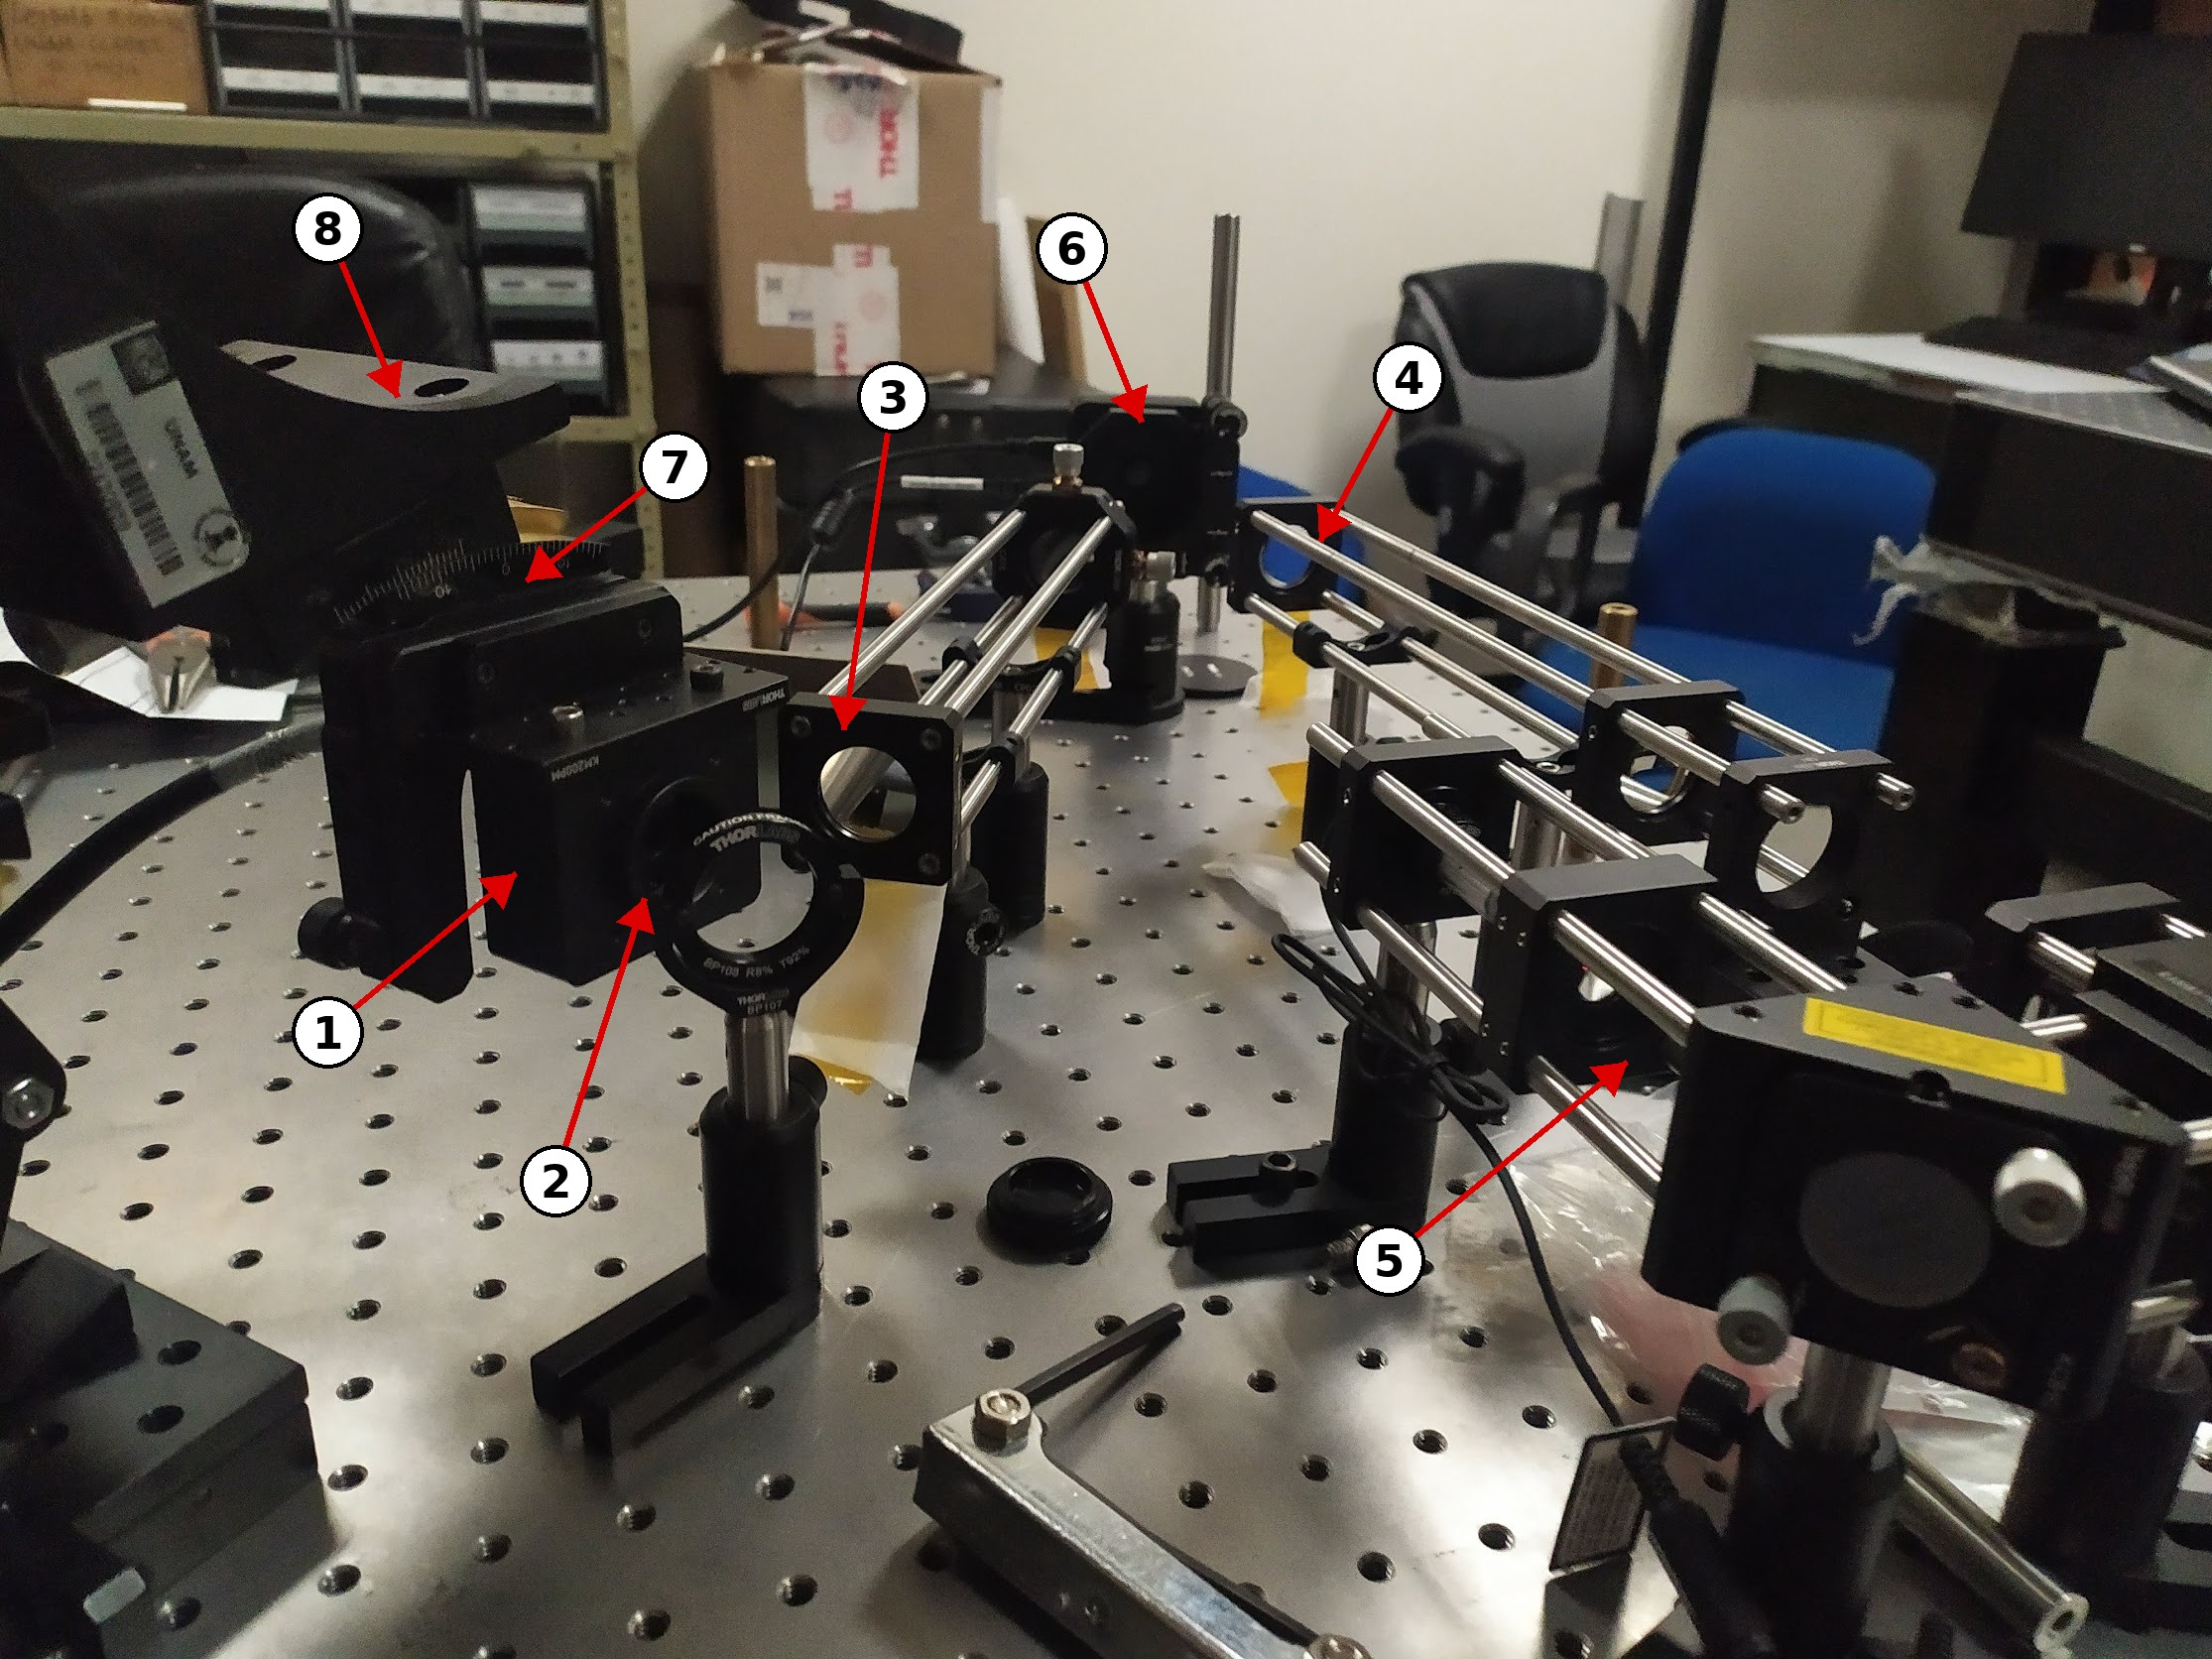
\includegraphics[width=\linewidth]{fotos/foto-divisor-sensor-anotada.jpg}
	\caption{Tramo final del sistema óptico. (1) Sensor WFS20-5C en su montura de
	inclinación; (2) divisor de haz de película delgada BP108 (R 8~\% / T 92~\%); (3) última
	placa de jaula del kit antes del divisor; (4) barras de jaula de las secciones del kit;
	(5) módulo de diodo láser (etiqueta de precaución); (6) espejo deformable DMP40-FM1, al
	fondo, al final de las secciones de jaula; (7) escala del goniómetro ($10\cdot 0\cdot
	10$); (8) placa fija de $90^\circ$ del subsistema de posicionamiento.}
	\label{fig:foto-divisor}
\end{figure}

El esquema del kit se mostró en la Fig.~\ref{fig:optica-adaptativa}; las
Figs.~\ref{fig:foto-montaje} y~\ref{fig:foto-divisor} muestran el montaje real.

\subsection{Convención de Zernike del software de control y modos evaluados}\label{sec:convencion-zernike}

Los índices $Z_k$ con los que se designan los modos del espejo deformable en este trabajo corresponden a la numeración del software de control (Thorlabs, DMP40-FM1), que coincide con la del software del sensor (\textit{WFS Series Wavefront Analysis Software}). Ambos utilizan los polinomios de Zernike en la nomenclatura ANSI Z80.28-2010 \cite{ThorlabsAOKManual}, con la salvedad de que el índice único comienza en $Z_1$ (pistón) en lugar de $j=0$; es decir, $Z_k^{\text{Thorlabs}} = Z_{j}^{\text{ANSI}}$ con $k = j + 1$. En esta convención, el polinomio de índices radial $n$ y meridional $m$ es
\begin{equation}
Z_n^m(\rho,\theta) = N_n^m\, R_n^{|m|}(\rho)\, M(m\theta),
\qquad
N_n^m = \sqrt{(2-\delta_{0,m})(n+1)},
\label{eq:zernike-ansi}
\end{equation}
con $M(m\theta)=\cos(m\theta)$ para $m \ge 0$ y $M(m\theta)=\sen(|m|\theta)$ para $m < 0$. El software del espejo permite controlar los términos $Z_4$ a $Z_{15}$ con amplitudes relativas en el intervalo $[-1, +1]$.

Los dos modos del espejo activados en las evaluaciones del Capítulo~\ref{cap:resultados},
con su expresión analítica explícita y su nombre estándar, son los de la
Tabla~\ref{tab:modos-dm}. Nótese que en el índice ANSI base 0 el valor $j=13$ corresponde
al astigmatismo secundario-$x$, un modo distinto del $Z_{13}$ del software; la relación
$k=j+1$ resuelve esta ambigüedad de numeración.

\begin{table}[htbp]
\centering
\caption{Modos del espejo deformable evaluados en este trabajo. El índice $Z_k$ es el del
software de Thorlabs (pistón $=Z_1$); $j$ es el índice único ANSI equivalente.}
\label{tab:modos-dm}
\setlength{\tabcolsep}{4pt}
\begin{tabularx}{\textwidth}{cccc>{\raggedright\arraybackslash}X}
\hline
\textbf{Modo del DM} & $\boldsymbol{j}$ \textbf{(ANSI)} & $\boldsymbol{(n,m)}$ & \textbf{Forma analítica} & \textbf{Nombre} \\
\hline
$Z_{11}$ (\textit{TetY}) & $10$ & $(4,-4)$ & $\sqrt{10}\,\rho^4\sen 4\theta$ & Tetrafoil-$y$ \\
$Z_{13}$ (\textit{SAb3}) & $12$ & $(4,0)$  & $\sqrt{5}\,(6\rho^4-6\rho^2+1)$ & Esférica primaria \\
\hline
\end{tabularx}
\end{table}

\section{Sistema de control y adquisición de datos}\label{sec:control-adquisicion}

El sistema de control y adquisición de datos utilizado en el experimento está compuesto
por una computadora desde la cual se operan simultáneamente tres interfaces de software.
La primera corresponde al software del sensor Shack-Hartmann provisto por Thorlabs
(\textit{WFS Series Wavefront Analysis Software}), que permite visualizar el patrón de
spots, la vista del haz, la reconstrucción del frente de onda y los coeficientes de
Zernike, además de reportar métricas como PV (pico-valle), RMS (valor cuadrático medio) y
wRMS (RMS ponderado). Esta misma interfaz permite registrar y exportar los datos de
centroides asociados a cada microlente para cada corrimiento. En este trabajo no se
desarrolló ni se modificó la rutina de detección de centroides: el cálculo de centroides
es propio del software del fabricante y aquí se utiliza tal cual; lo que se desarrolla en
los capítulos siguientes es la reconstrucción del frente de onda a partir de esos
centroides mediante el método de corrimiento de puntos. Más adelante se compara el
resultado del método propuesto con la reconstrucción Zernike que el propio software
entrega, como referencia cuantitativa (RMS). La segunda interfaz corresponde al control
del espejo deformable, desde donde se imponen aberraciones del frente de onda mediante
amplitudes y combinaciones de modos Zernike. La tercera es el software APT asociado al
controlador KDC101 de la platina MTS50-Z8, utilizado para programar la distancia de
desplazamiento, ejecutar cada corrimiento y monitorear la posición del actuador durante la
medición.

\section{Fuente de luz}

El haz de luz utilizado en el experimento (Fig.~\ref{fig:generacion-haz}) es el del módulo
de diodo láser incluido en el kit de óptica adaptativa: 635 nm de longitud de onda y 0.30
mW de potencia (láser Clase 1) \cite{ThorlabsAOKManual}. La expansión y colimación del haz
corren a cargo de la primera sección del propio kit, descrita en la Sección del Sistema
óptico: a la salida de ese subsistema el haz es, por diseño del kit, colimado y de un
diámetro que cubre la apertura del espejo deformable, que es justamente el requisito del
experimento: disponer de un frente de onda nominalmente plano sobre la superficie activa
del espejo. Las secciones se usaron prealineadas de fábrica y la colimación no se midió
por separado (Sección~\ref{sec:sistema-optico}). Con ese haz colimado dentro del sistema
óptico adaptativo: cuando el espejo deformable se encuentra relajado (plano) actúa como un
simple espejo plano y el frente de onda que llega al sensor Shack-Hartmann sigue siendo
plano; cuando los actuadores deforman su superficie, el frente de onda reflejado se
modifica de forma controlada antes de incidir en el sensor.

\begin{figure}[H]
	\centering
	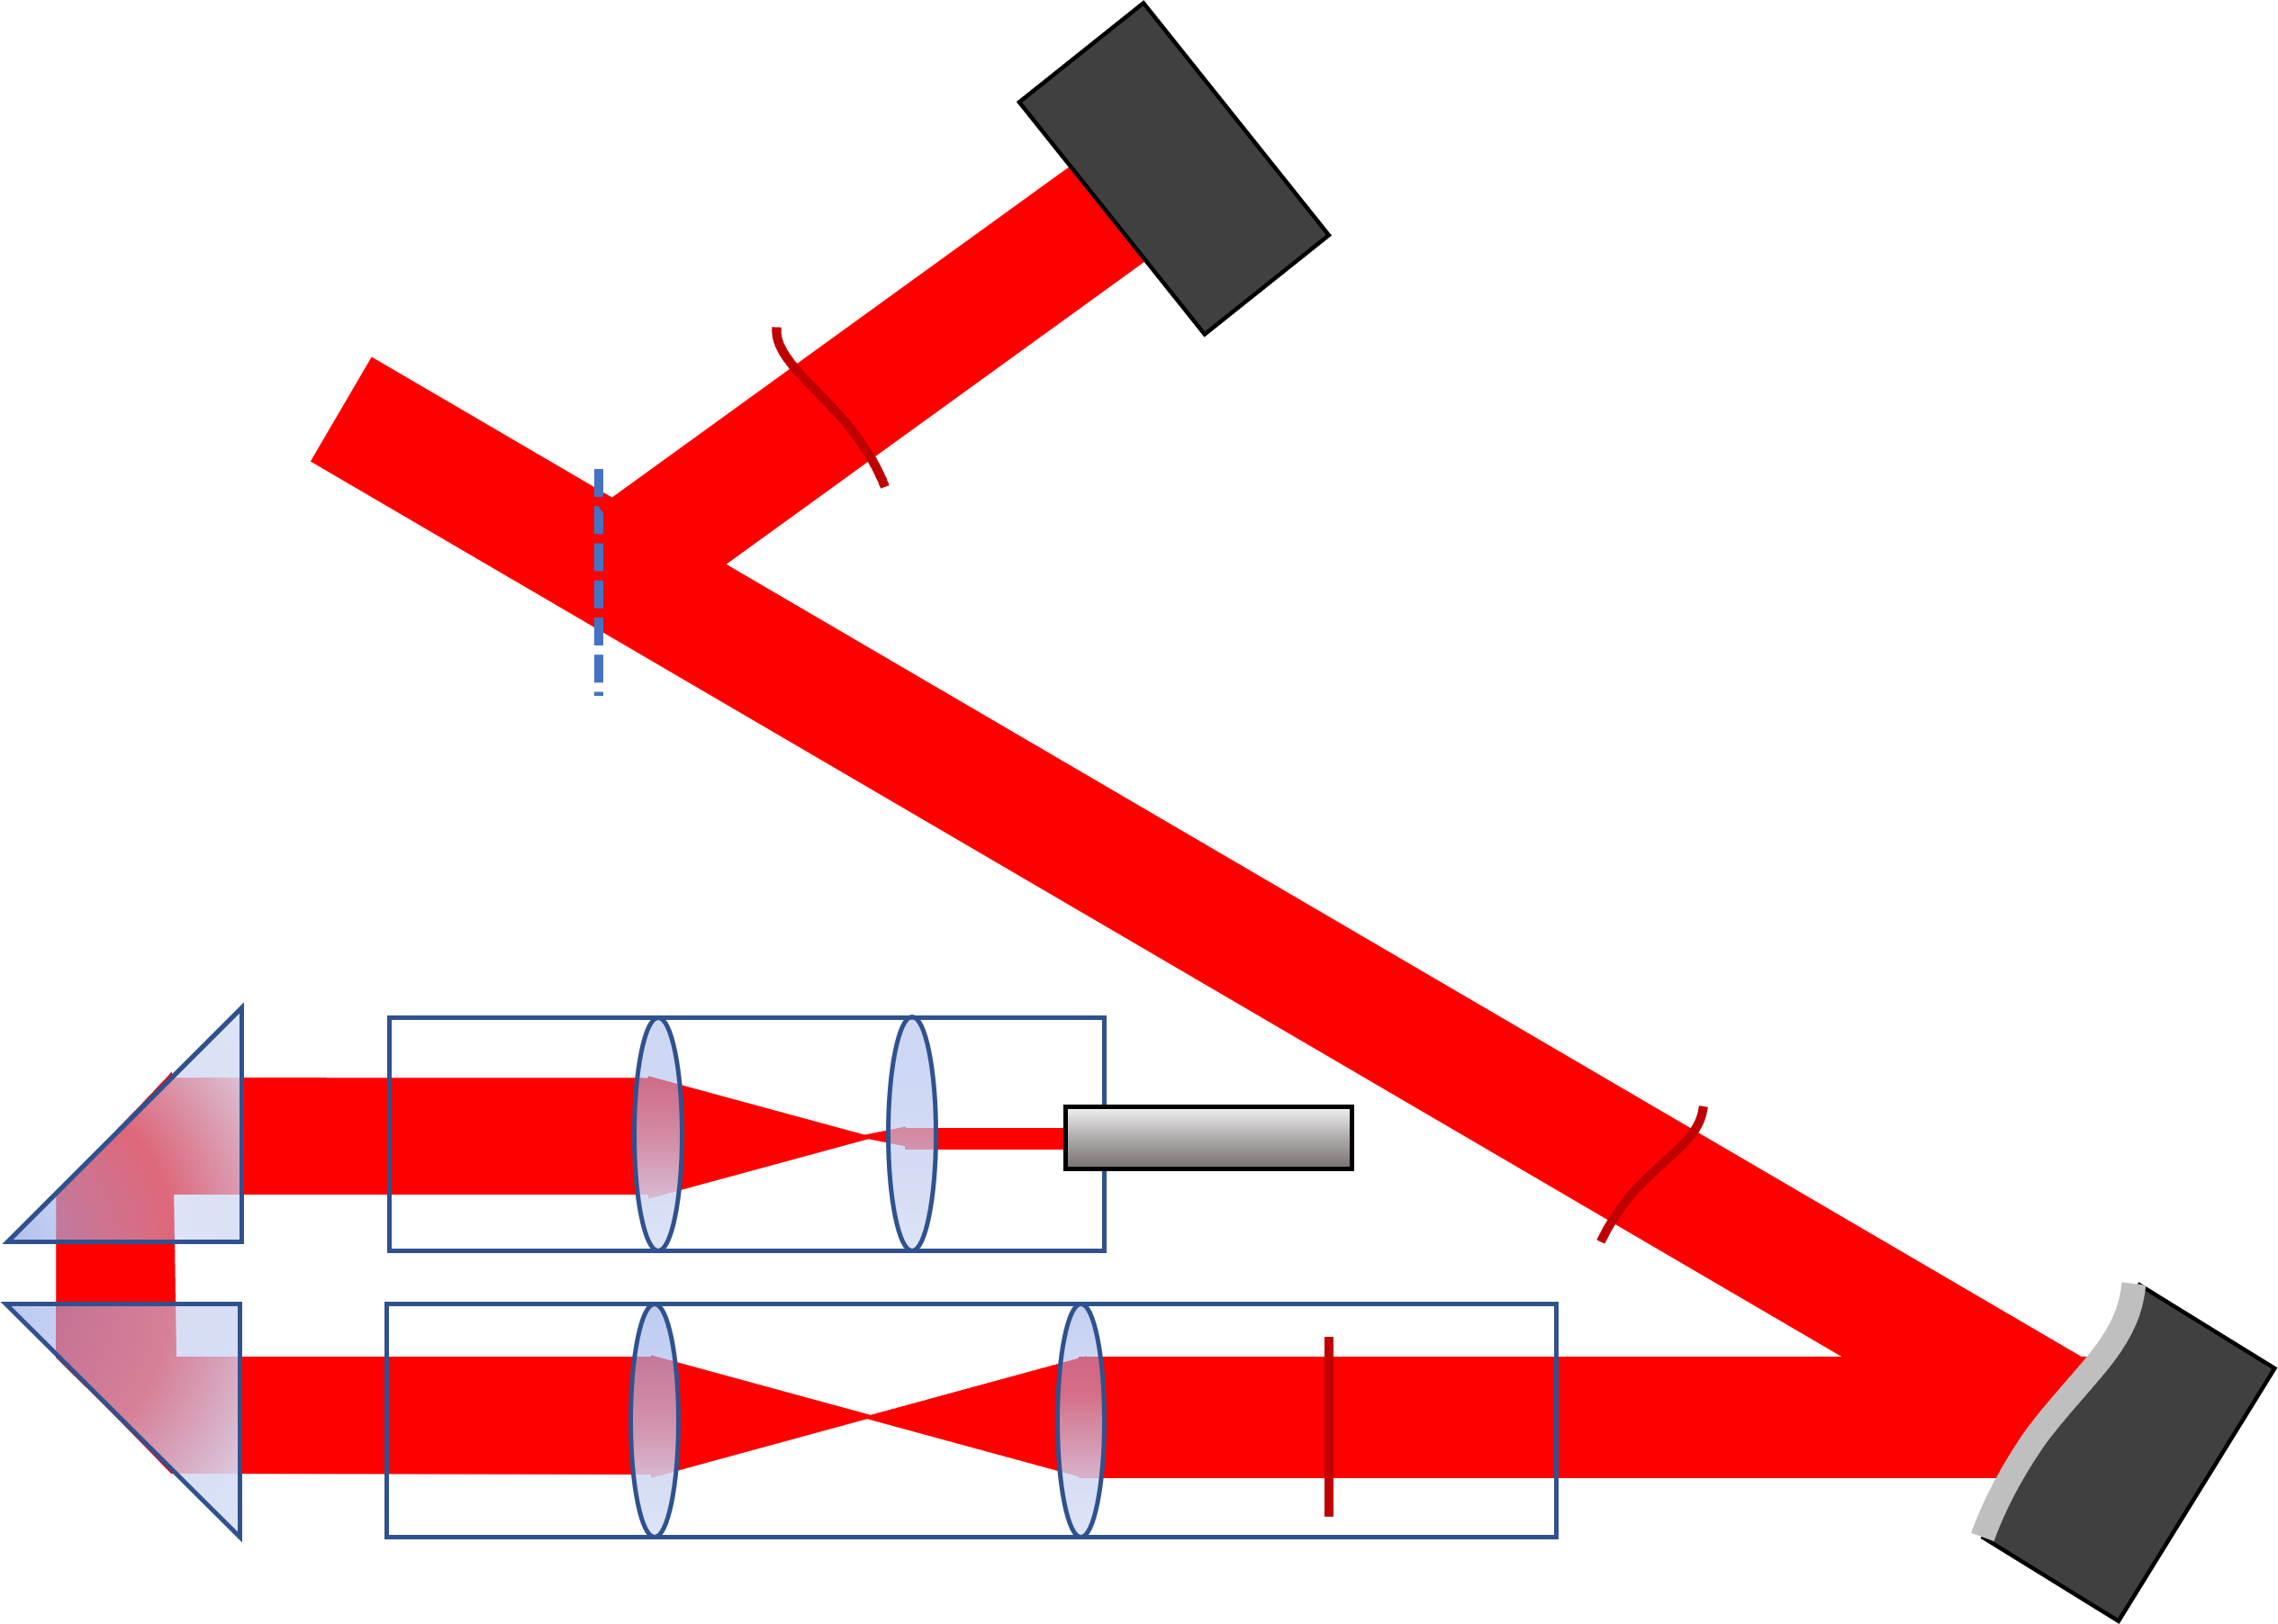
\includegraphics[width=0.5\linewidth]{GeneracionDelHaz.png}
	\caption{Generación del haz de luz utilizado en el experimento}
	\label{fig:generacion-haz}
\end{figure}

\section{Resumen}

En este capítulo se ha detallado el arreglo experimental utilizado para la evaluación por
el método Shack-Hartmann con corrimiento de puntos. Se ha explicado el funcionamiento del
sensor Shack-Hartmann, el sistema de óptica adaptativa, el sistema de control y
adquisición de datos, la generación del haz de luz, y la montura y control del sensor.

La integración de estos componentes forma un sistema que permite implementar el método de
corrimiento de puntos para mejorar la resolución transversal del sensor Shack-Hartmann. El
sistema de posicionamiento proporciona los grados de libertad necesarios para realizar los
desplazamientos controlados del sensor, mientras que el sistema óptico adaptativo basado
en el espejo deformable permite generar frentes de onda aberrados de forma controlada para
validar el método.

La alineación cuidadosa de todos los componentes asegura la precisión y reproducibilidad
de las mediciones, aspectos fundamentales para demostrar las ventajas del método de
corrimiento de puntos en la caracterización de frentes de onda ópticos.

En los próximos capítulos se explicará en detalle la metodología de evaluación y se
presentarán los resultados obtenidos con este sistema experimental.

\chapter{Metodología de evaluación}\label{cap:metodologia}
\section{Procedimiento experimental}

\subsection{Paso 1: Ajuste del ángulo de barrido}\label{sec:ajuste-angulo}

Experimentalmente, el primer paso de la metodología consiste en ajustar con precisión el
ángulo para el barrido deseado. Para ilustrar el procedimiento, describiremos una
evaluación específica con dirección $(m,n) = (1,2)$, que corresponde a un ángulo $\theta_r
= \arctan(m/n) \approx 26.57^\circ$ según la Ec.~\ref{Eq: angulo}, valor matemáticamente
exacto que se redondea a $26.6^\circ$ por presentación. Para el método de corrimiento de
puntos importa únicamente la \emph{dirección} (entendida como la recta infinita definida
por el ángulo $\theta$ sobre el plano coordenado, análoga a la dirección $x$ o $y$) y no
el \emph{sentido} en que se recorre. Sumar $180^\circ$ al ángulo no cambia la dirección:
mantiene la misma recta y sólo invierte cuál mitad se toma como positiva. Por ello $\theta
\approx 26.57^\circ$ y $\theta + 180^\circ \approx 206.57^\circ$ son equivalentes y
generan el mismo reticulado final. Sin embargo, esta misma metodología se aplicó para
diferentes direcciones de barrido y números de corrimientos, adaptando los parámetros
según los requerimientos de cada experimento.

Antes de asignar valores angulares hay que fijar la convención de signos, pues el signo de
una rotación depende del punto de vista del observador. En este trabajo los ángulos se
refieren a un observador que mira en la misma dirección en que observa el lente de la
cámara (a lo largo de su eje óptico), tomando como referencia el eje de desplazamiento; en
esa referencia, las contribuciones de la platina fija y de la AP180 resultan negativas, y
la corrección del goniómetro toma el signo que requiera cada dirección. Si el sistema se
observa de frente a la cámara, los mismos giros cambian de signo; las magnitudes, desde
luego, son las mismas (en el Capítulo~3 los componentes se describieron por su magnitud,
sin signo).

Hay que considerar que la posición inicial de la cámara está invertida a $-180^\circ$ (ver
Fig.~\ref{fig:invertido-met}). Esta orientación se construye apilando dos elementos del
sistema de control angular descrito en el Capítulo~3: una platina fija de $-90^\circ$,
sobre la que se monta la platina de rotación de ángulo ajustable (AP180) también a
$-90^\circ$, sumando $-180^\circ$ en total. Esta inversión inicial es deliberada, pues
sirve como punto de partida para generar el ángulo de barrido sumándole inclinación.

Gracias a esta inversión, para obtener la dirección de barrido $(1,2)$ basta con añadir
$26.6^\circ$ a la posición de referencia. Como la AP180 sólo se fija cada $15^\circ$, esto
se hace en dos pasos: la AP180 pasa de $90^\circ$ a $60^\circ$ hacia abajo, es decir,
aporta un giro grueso de $30^\circ$ (dos pasos), y el goniómetro retrocede $3.4^\circ$ en
sentido contrario, con lo que el sensor queda a $26.6^\circ$ de la referencia. Para la
dirección $(1,3)$, con $\theta_r \approx 18.4^\circ$, la AP180 aporta un paso de
$15^\circ$ y el goniómetro añade los $3.4^\circ$ restantes. En todos los casos la
corrección del goniómetro queda dentro de su recorrido de $\pm 10^\circ$. Para otras
direcciones de barrido, los ángulos se calculan con la Ec.~\ref{Eq: angulo} y se ajustan
siguiendo el mismo procedimiento.

Rotar la platina AP180 modifica la altura efectiva del sensor respecto al plano del haz,
ya que el centro de giro del conjunto no coincide con el plano de detección. Para mantener
al sensor sobre el plano de propagación del haz a lo largo del barrido, se utiliza la mesa
de altura variable L490 descrita en la Sección~\ref{sec:control-desplazamiento-altura},
ajustando la altura tras cada cambio de ángulo. Esta corrección no forma parte del método
teórico (Capítulo~2), sino del montaje físico requerido para implementarlo.

\begin{figure}[htbp!]
	\centering
	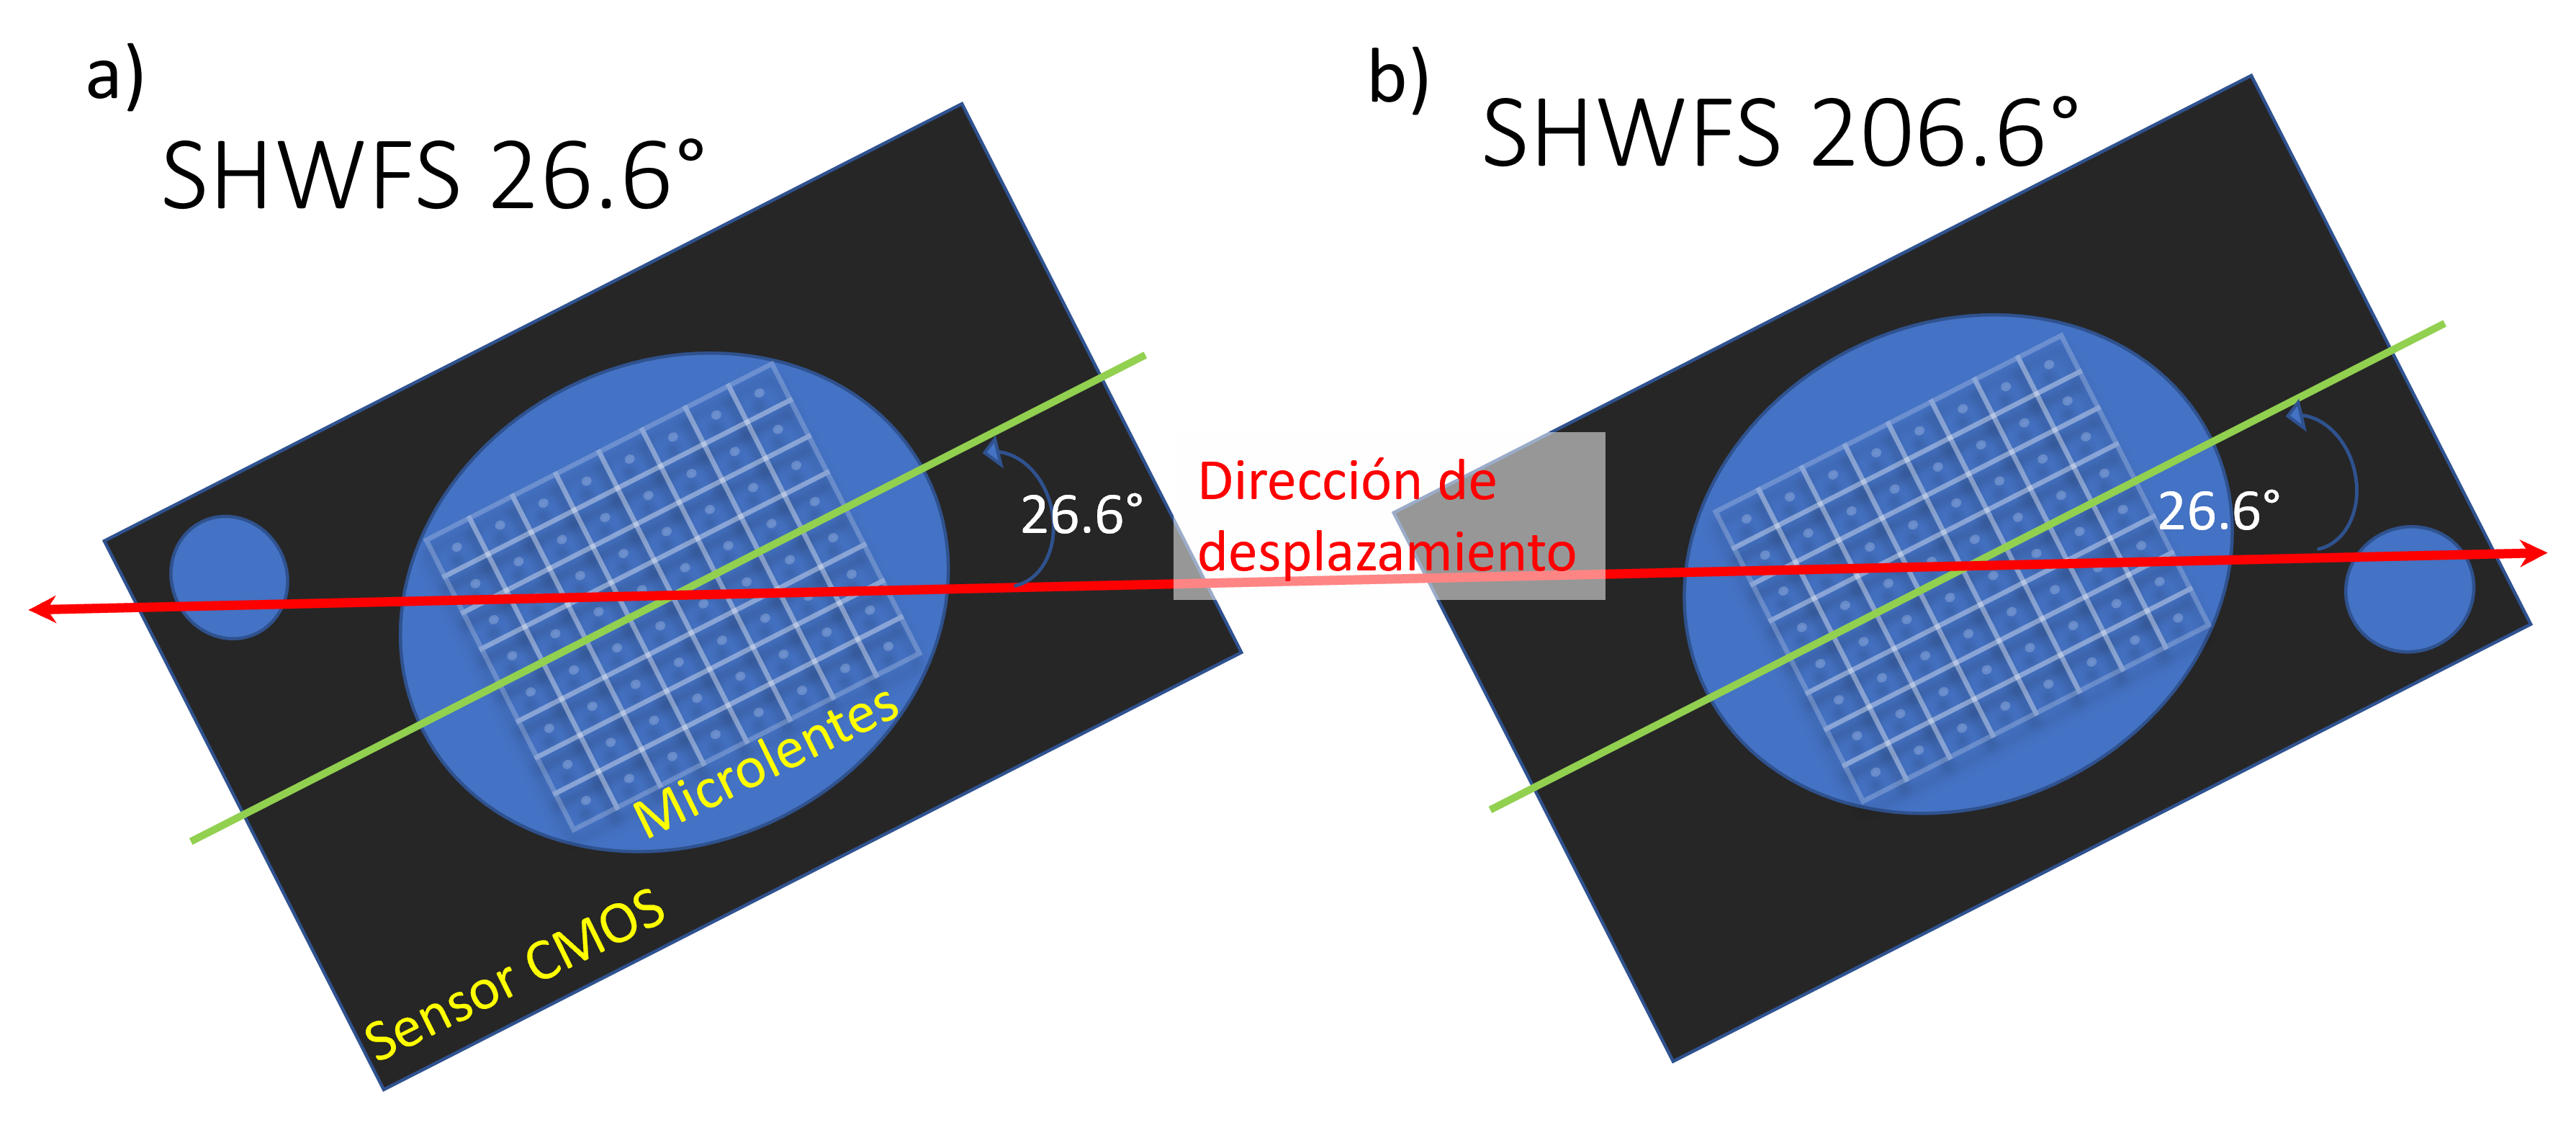
\includegraphics[width=0.7\linewidth]{fig.invertido.png}
	\caption{Evaluación con dirección $(m,n)=(1,2)$: a) recorrido en el sentido $\theta_r
	\approx 26.6^\circ$; b) recorrido en el sentido opuesto $\theta_r+180^\circ \approx
	206.6^\circ$, obtenido con la cámara invertida. Ambas configuraciones definen la misma
	dirección (la misma recta) y generan el mismo reticulado; sólo difieren en cuál sentido
	se toma como positivo.}
	\label{fig:invertido-met}
\end{figure}

\subsection{Paso 2: Alineación del sistema}\label{sec:alineacion-sistema}

Una vez establecido el ángulo de barrido, el siguiente paso crítico es alinear con
precisión el haz láser para que incida centralmente sobre el sensor. Esta alineación se
realiza utilizando el software del fabricante (\textit{WFS Series Wavefront Analysis
Software}, Thorlabs; descrito en la Sección~\ref{sec:control-adquisicion}), que permite
visualizar en tiempo real el centroide de la intensidad lumínica captada por el sensor.
Mediante esta herramienta se ajustan la altura y la posición del sensor hasta que el haz
queda centrado en la apertura del arreglo de microlentes, usando como guía el círculo de
la pupila y el centroide global que muestra el software. Se trata de un centrado visual,
sin un punto de referencia absoluto, de modo que la posición inicial no se reproduce
exactamente de una evaluación a otra; lo que el método requiere es que esa posición se
mantenga durante el barrido, no que coincida entre evaluaciones.

Durante este proceso de alineación el espejo deformable ya se encuentra en posición dentro
del montaje óptico, pero configurado en su estado plano, es decir, sin aplicar ningún
índice de deformación. Esto permite que el espejo actúe simplemente como un espejo plano,
sin introducir aberraciones al haz durante la fase de alineación del sistema.

\subsection{Paso 3: Deformación del frente de onda}

El tercer paso consiste en generar una deformación controlada del frente de onda plano que
entrega el kit. Si bien existen diversos métodos para lograr esto, como la introducción de
una lente bajo evaluación o un sistema óptico completo, para este trabajo se optó por
utilizar el espejo deformable DMP40-FM1 integrado en el sistema de óptica adaptativa,
gobernado desde el software de control del espejo de Thorlabs
(Sección~\ref{sec:convencion-zernike}), en el que se selecciona el modo de Zernike y la
amplitud de su deslizador; las configuraciones utilizadas en las evaluaciones se listan en
la Tabla~\ref{tab:modos-dm}. Esta elección permite un control reproducible sobre las
aberraciones introducidas en el haz láser, facilitando así la evaluación del método de
corrimiento de puntos.

\subsection{Paso 4: Adquisición de datos}\label{sec:adquisicion-datos}

Con el sistema correctamente configurado y alineado, se procede a la adquisición de datos
utilizando el software de Thorlabs específicamente calibrado para el sensor Shack-Hartmann
empleado. Este software proporciona información detallada sobre los centroides de
intensidad asociados a cada microlente del arreglo. La Fig.~\ref{fig:shg-crudo} muestra
ejemplos del Shack-Hartmanngrama en crudo registrado por el sensor en distintas
configuraciones del espejo deformable, manteniendo fija la dirección de barrido.

Para realizar los desplazamientos secuenciales, se programa el servomotor con la distancia
de movimiento calculada según la Ec.~\ref{eq:distdesp} para la dirección seleccionada. El
número de corrimientos depende directamente de los valores $m$ y $n$ elegidos, según la
relación $\varepsilon = m^2 + n^2$, lo que permite adaptar la densidad del muestreo a las
necesidades específicas de cada evaluación.

\begin{figure}[htbp!]
	\centering
	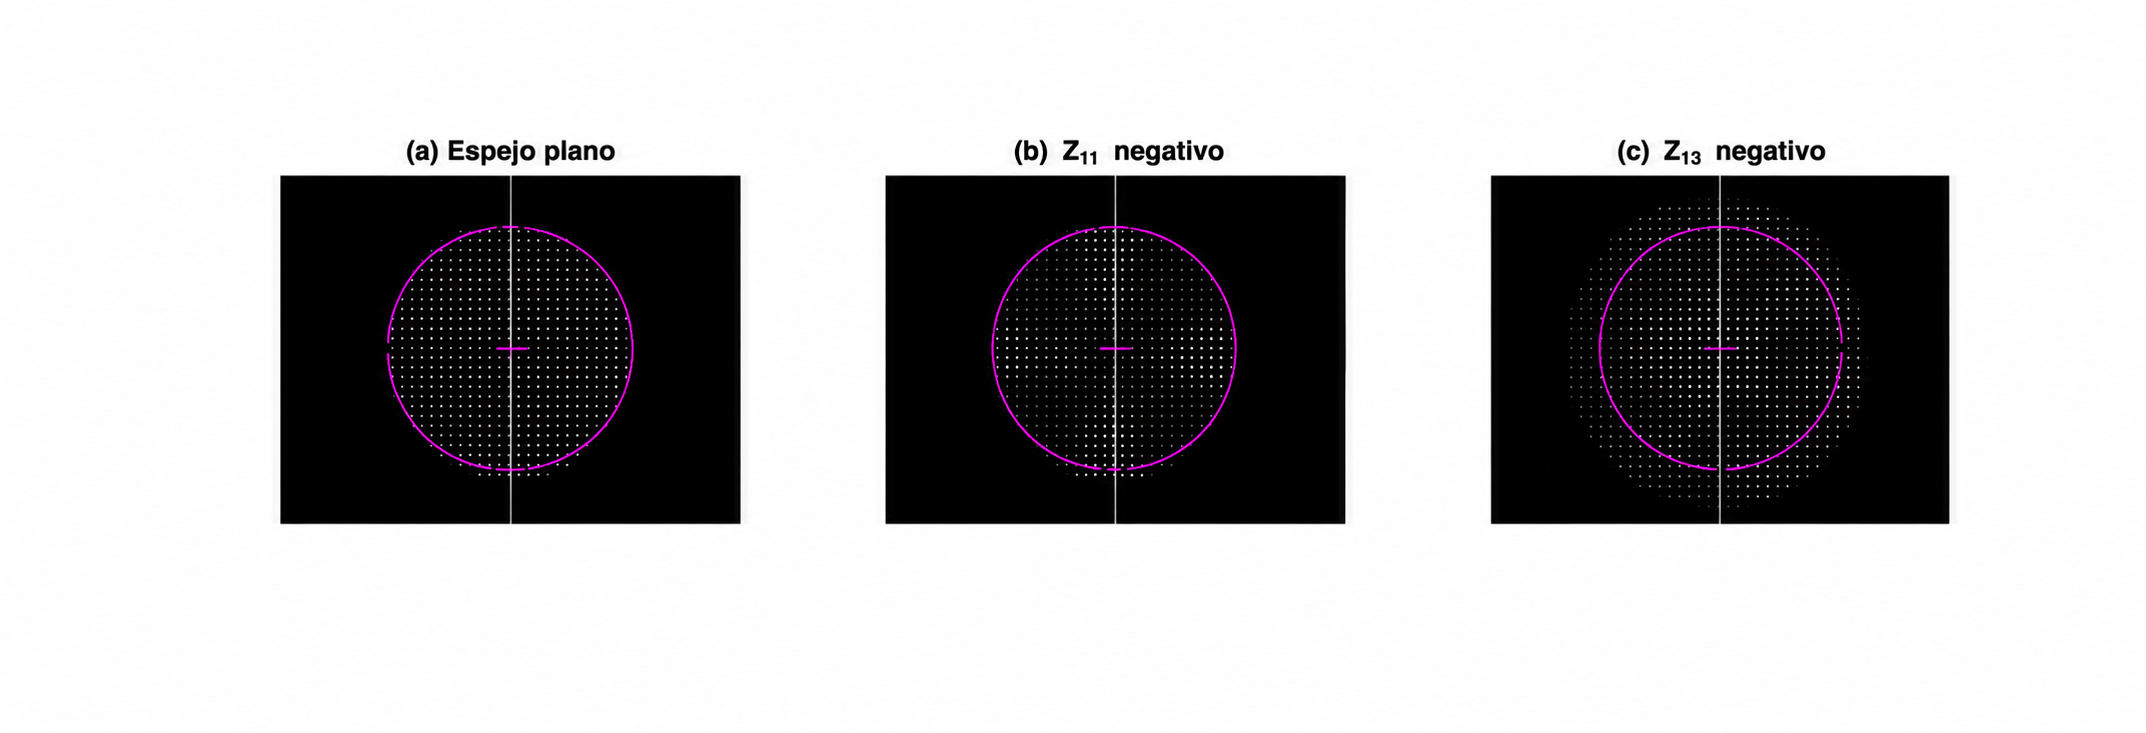
\includegraphics[width=\linewidth]{cap4-shg-crudo-2.png}
	\caption{Shack-Hartmanngramas en crudo del sensor para tres configuraciones del espejo
	deformable, todas con dirección de barrido $(m,n)=(1,2)$ y corrimiento central
	($\sigma=0$): a) espejo plano (referencia sin aberración); b) modo Zernike $Z_{11}$
	(tetrafoil) con amplitud negativa ($-0.99$); c) modo Zernike $Z_{13}$ (esférica primaria)
	con amplitud negativa ($-0.97$) (convención y formas analíticas en la
	Tabla~\ref{tab:modos-dm}). El círculo y la cruz superpuestos provienen del software de
	adquisición de Thorlabs y delimitan la pupila y el centro óptico del sensor.}
	\label{fig:shg-crudo}
\end{figure}

Cada desplazamiento se realiza en condiciones controladas de laboratorio, con la
iluminación ambiental apagada para minimizar la luz espuria. Este procedimiento se repitió
de manera consistente para todas las configuraciones de barrido evaluadas en este trabajo.

Antes de cada evaluación, con el espejo deformable en su estado plano, se ajustan la
altura y la posición del sensor hasta que el haz incide centrado sobre el arreglo de
microlentes; esa posición define la captura central (\texttt{d+0}). Los corrimientos se
realizan después en ambos sentidos a partir de ella (primero negativos, luego positivos)
en lugar de avanzar $\varepsilon$ pasos en un solo sentido, de modo que las posiciones
muestreadas queden distribuidas alrededor del centro del haz; esto no cambia el patrón
resultante, pero aprovecha mejor la región central, dado que el arreglo de microlentes es
finito.

En cada posición del barrido se captura y almacena un archivo con los datos de los centroides. Los archivos se nombran con el patrón \texttt{cent d$\pm$k $\pm$NNNN.csv}, donde:
\begin{itemize}
	\item \texttt{cent} indica que el archivo contiene centroides; con el mismo patrón se guardan el mallado de reconstrucción del fabricante (\texttt{mesh}), la distribución de potencia por microlente (\texttt{pow}) y la imagen del spotgrama (\texttt{.bmp});
	\item \texttt{d$\pm$k} es el índice del corrimiento, con signo según el sentido del desplazamiento (\texttt{d+0} es la posición central);
	\item \texttt{$\pm$NNNN} es el desplazamiento acumulado respecto a la posición central, en décimas de micra (\texttt{+0671} corresponde a $+0.0671$~mm y \texttt{-1342} a $-0.1342$~mm).
\end{itemize}
Por ejemplo, la evaluación en la dirección $(1,2)$ produce los archivos \texttt{cent d-2 -1342.csv}, \texttt{cent d-1 -0671.csv}, \texttt{cent d+0 +0000.csv}, \texttt{cent d+1 +0671.csv} y \texttt{cent d+2 +1342.csv}. Simultáneamente, se registran las condiciones de control del espejo deformable para asegurar la trazabilidad y reproducibilidad de las mediciones.

Finalmente, tras recopilar todos los archivos CSV de centroides correspondientes a los
$\varepsilon = m^2 + n^2$ pasos de la evaluación, esta información se procesa y se
organiza. A la lista de centroides de cada corrimiento $k$ se le suma el vector de
desplazamiento del sensor en esa captura, $(\sigma_k\cos\theta,\ \sigma_k\sen\theta)$, de
modo que todos los centroides queden expresados en un mismo sistema de coordenadas; al
concatenar las $\varepsilon$ listas así desplazadas se obtiene el patrón densificado
(Sección~\ref{sec:composicion-corrimientos}). Sin embargo, a menudo el archivo de
centroides puede contener puntos adicionales originados por regiones de baja intensidad
lumínica o por luz espuria, como se muestra en la Fig.~\ref{fig:seleccion-met}~a). Por
esta razón, se restringe el análisis a una región circular que corresponde al haz real; el
criterio con que se fija su radio se describe en la Sección~\ref{sec:seleccion-region}. De
esta acción resultan los puntos delimitados que representan la región específica que se
desea estudiar.

\begin{figure}[htbp!]
	\centering
	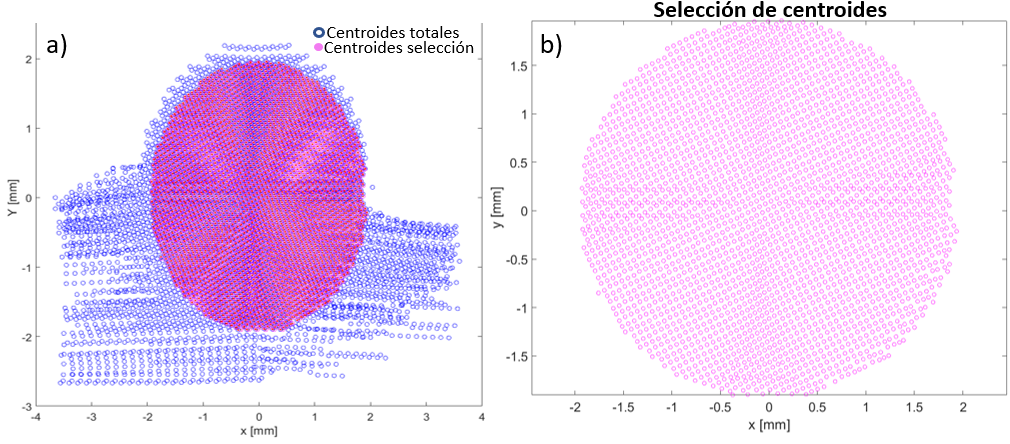
\includegraphics[width=0.9\linewidth]{Selección.png}
	\caption{a) Centroides totales arrojados por el software de Thorlabs en azul y la
	selección del área del haz en rosa; b) selección final de centroides, se puede observar
	la acumulación de puntos en algunas zonas efecto de la deformación del frente de onda}
	\label{fig:seleccion-met}
\end{figure}


Utilizando estos puntos, que ya se encuentran relacionados con la posición central de la
microlente que los generó, se obtienen los caminos de integración y, a partir de ellos, se
procede a integrar la aberración transversal para obtener el frente de onda o la
aberración del frente de onda.

\section{Recuperación y tratamiento de datos}

Para cada corrimiento, el software de Thorlabs entrega un archivo \texttt{CSV} con las
posiciones $(x,y)_{\text{pix}}$ de los centroides de cada microlente del arreglo. Esta
sección describe cómo, a partir de esos $\varepsilon$ archivos en crudo, se obtiene la
lista única de pendientes locales que alimenta la integración numérica. El procesamiento
se descompone en cuatro etapas: definición de los datos de entrada y las constantes del
sensor (Sección~\ref{sec:datos-entrada}), conversión de los centroides a aberración
transversal (Sección~\ref{sec:cent-a-aberracion}), composición de los $\varepsilon$
corrimientos en un patrón densificado (Sección~\ref{sec:composicion-corrimientos}) y
selección de la región útil (Sección~\ref{sec:seleccion-region}).

\newpage

\subsection{Datos de entrada y constantes del sensor}\label{sec:datos-entrada}

\begin{figure}[htbp]
  \centering
  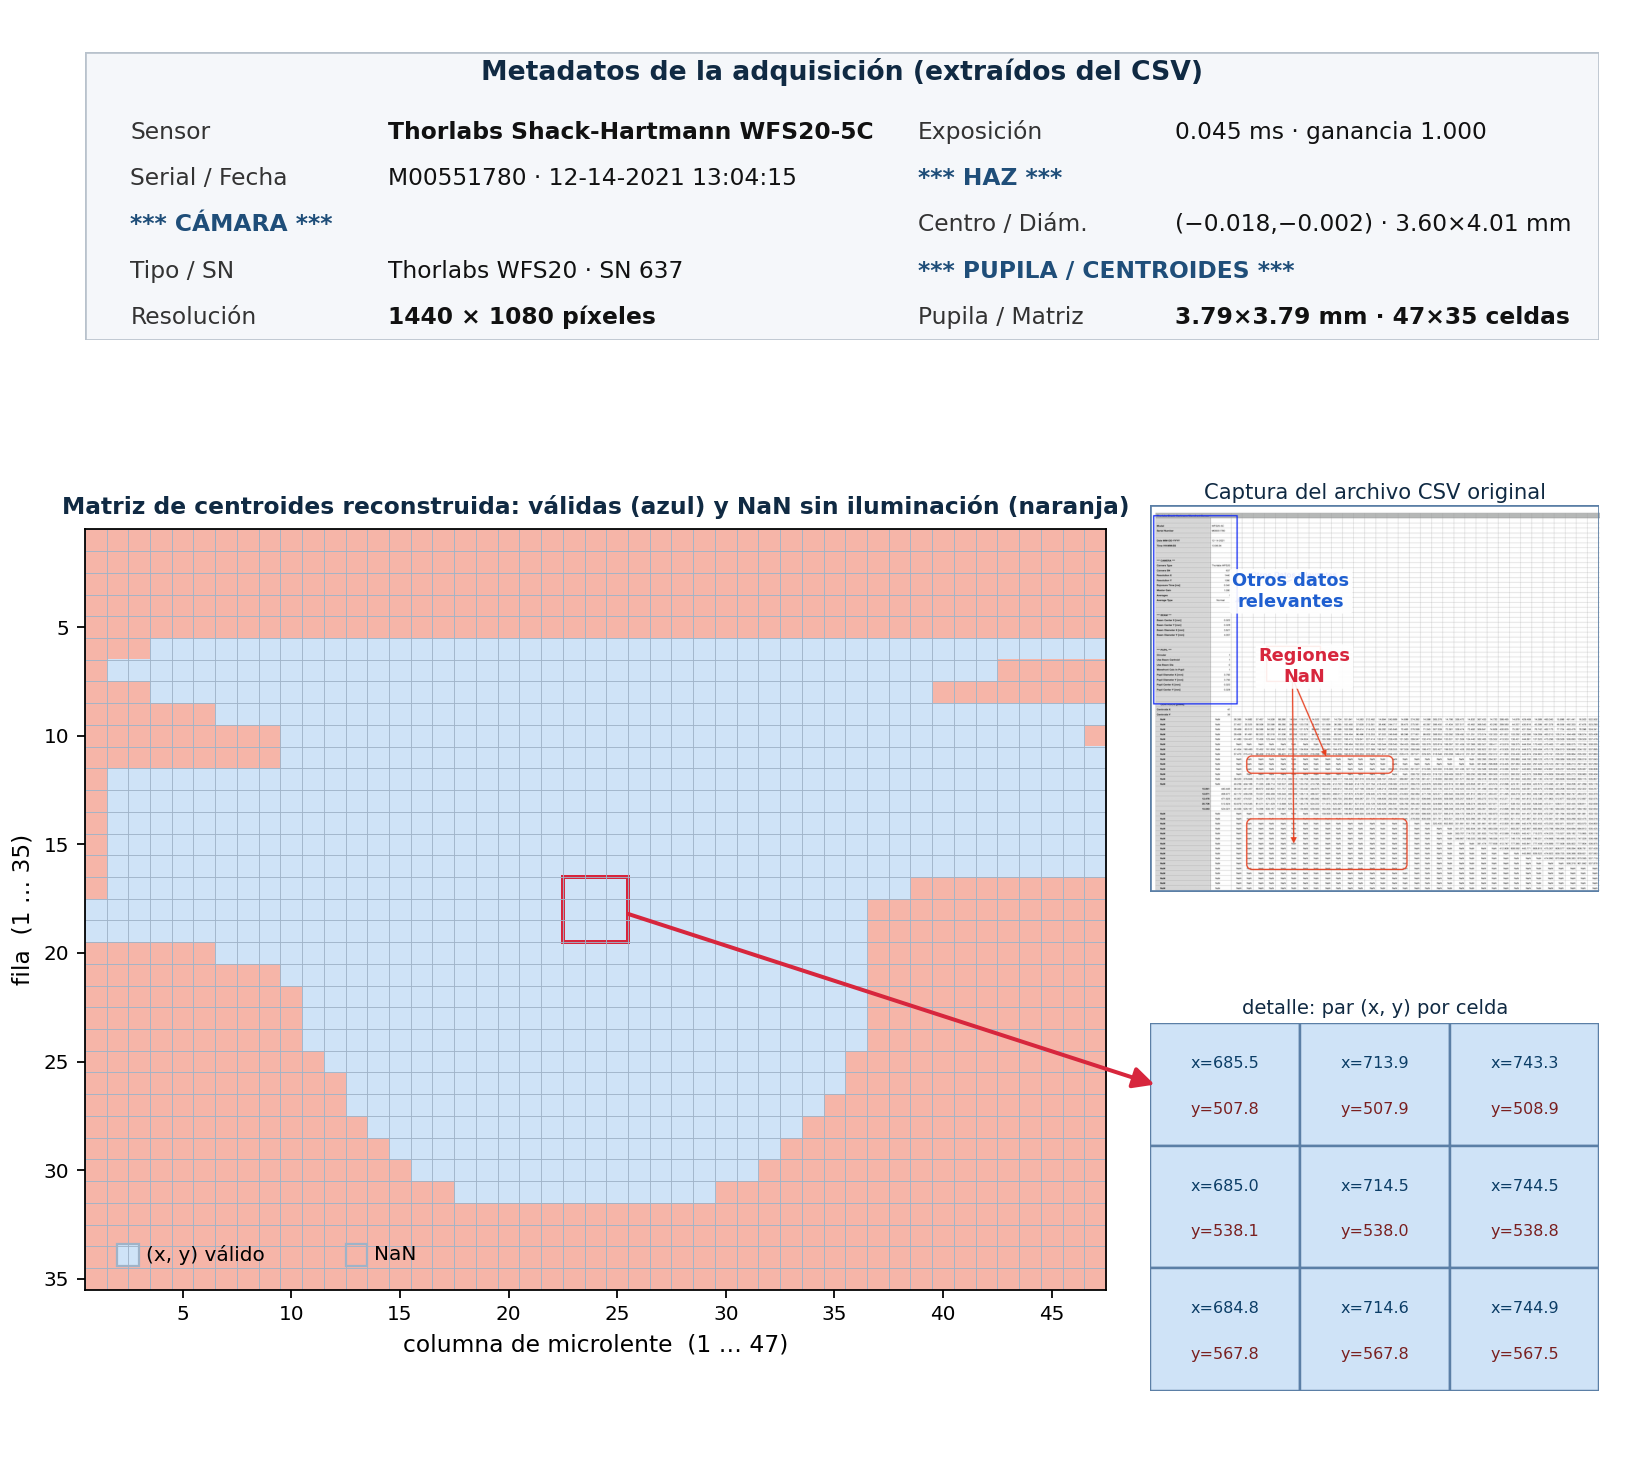
\includegraphics[width=0.9\linewidth]{cap4-centroides-nan-v2.png}
  \caption{Datos de centroides del archivo \texttt{CSV} que entrega el software de
  Thorlabs (captura original arriba a la derecha). De ese archivo se extraen los metadatos
  de la adquisición (arriba a la izquierda) y la matriz de $47\times35$ microlentes: cada
  celda guarda el par de coordenadas $(x,y)$ del centroide en píxeles (detalle a la
  derecha) y las celdas \texttt{NaN} corresponden a microlentes sin iluminación válida,
  fuera del haz, que se descartan durante el procesamiento
  (Sección~\ref{sec:cent-a-aberracion}). La representación gráfica de la matriz se
  reconstruyó a partir de los pares ordenados del archivo con ayuda de inteligencia
  artificial.}
  \label{fig:centroides-nan}
\end{figure}

La entrada al procesamiento son los $\varepsilon$ archivos \texttt{CSV} generados por el
software de Thorlabs, uno por cada posición de corrimiento. Cada archivo contiene una
matriz de pares ordenados $(x,y)_{\text{pix}}$ correspondientes a los centroides de las
microlentes del arreglo. El software ya está calibrado para el número de microlentes del
sensor, de modo que cada celda de la matriz queda asociada a una microlente específica.
Aquellas celdas correspondientes a microlentes con iluminación insuficiente o saturada
aparecen marcadas como nulas (\texttt{NaN}). La Fig.~\ref{fig:centroides-nan} muestra un
archivo real de centroides abierto como hoja de cálculo: el encabezado concentra los
metadatos de la adquisición (modelo y número de serie del sensor, parámetros de la cámara,
del haz y de la pupila), y la matriz inferior contiene las posiciones de los centroides,
con regiones de celdas \texttt{NaN} en las zonas del arreglo sin iluminación válida,
típicamente fuera del área del haz o en sus bordes.

Los centroides se entregan en el sistema de coordenadas del sensor: el origen $(0,0)$ de
nuestro sistema coordenado se ubica en la esquina superior izquierda del arreglo de
píxeles, con $x$ creciendo hacia la derecha y $y$ creciendo hacia abajo. Para convertir
cada centroide a coordenadas espaciales reales, así como para reconstruir la posición de
los centros de las microlentes, se utilizan las constantes geométricas y ópticas del
sensor WFS20-5C que se listan en la Tabla~\ref{tab:constantes-sensor}.

\begin{table}[htbp]
\centering
\caption{Constantes del sensor Shack-Hartmann WFS20-5C utilizadas en el procesamiento.}
\label{tab:constantes-sensor}
\begin{tabular}{l l l}
\hline
Símbolo & Descripción & Valor \\
\hline
$P_{sx}$ & Tamaño del píxel en $x$ & $5\,\mu\text{m}$ \\
$P_{sy}$ & Tamaño del píxel en $y$ & $5\,\mu\text{m}$ \\
$N_x$ & Número de píxeles del sensor en $x$ & $1440$ \\
$N_y$ & Número de píxeles del sensor en $y$ & $1080$ \\
$P_L$ & Distancia entre microlentes (\textit{lens pitch}) & $150\,\mu\text{m}$ \\
$f$ & Distancia focal de las microlentes & $4.1\,\text{mm}$ \\
\hline
\end{tabular}
\end{table}

\subsection{De centroides a aberración transversal}\label{sec:cent-a-aberracion}

A partir de la matriz de centroides en píxeles entregada por el software, esta etapa
produce, para cada corrimiento, una lista en la que cada renglón corresponde a una
microlente y contiene la posición del centroide medido, la posición del centro de la
microlente y la aberración transversal local. La transformación se realiza en cuatro
pasos.

\paragraph{Conversión a coordenadas espaciales.} Cada centroide $(x,y)_{\text{pix}}$ se lleva a coordenadas espaciales del sensor multiplicando por el tamaño del píxel:
\begin{equation}
x_c = x_{\text{pix}} \cdot P_{sx}, \qquad y_c = y_{\text{pix}} \cdot P_{sy}.
\label{eq:px-to-mm}
\end{equation}
Las celdas marcadas como nulas (microlentes sin iluminación válida) se conservan provisionalmente y se filtran al final de la etapa.

\paragraph{Cálculo de los centros de microlente.} Las posiciones de los centros de microlente no se miden: se reconstruyen a partir de la geometría conocida del arreglo. Las microlentes ocupan una retícula cuadrada de paso $P_L$ con 47 columnas en $x$ y 35 filas en $y$ sobre el sensor, de modo que sus centros nominales forman la malla
\begin{equation}
\bigl(x_\ell^{(i,j)}, y_\ell^{(i,j)}\bigr) = (i \cdot P_L + \delta_x, \; j \cdot P_L + \delta_y),
\quad i = 1,\dots,47, \quad j = 1,\dots,35,
\label{eq:lens-grid}
\end{equation}
donde $\delta_x, \delta_y$ son corrimientos de calibración que alinean la malla con la posición real del arreglo sobre el sensor. A continuación se traslada el origen de coordenadas a la microlente central del arreglo $(i,j)=(24,18)$, de modo que $(0,0)$ coincide con su centro:
\begin{equation}
(x,\,y) \;\leftarrow\; \bigl(x - x_\ell^{(24,18)},\; y - y_\ell^{(24,18)}\bigr).
\label{eq:traslacion-origen}
\end{equation}
La misma traslación se aplica tanto a los centros de microlente de la malla como a los centroides convertidos en el paso anterior, para que ambos conjuntos de coordenadas compartan origen.

\paragraph{Aberración transversal.} Siguiendo la definición dada en la Sección~\ref{sec:eval-clasica-SH} (Ec.~\ref{eq:aberracion-transversal-cap2}), la aberración transversal se calcula para cada microlente como
\begin{equation}
T_x = x_\ell - x_c, \qquad T_y = y_\ell - y_c.
\label{eq:aberracion-transversal}
\end{equation}
La relación con la pendiente local del frente de onda (Ec.~\ref{eq:pendiente-aberracion-cap2}) se utiliza más adelante en la integración numérica (Sección~\ref{sec:integracion}).

\paragraph{Filtrado de microlentes inválidas.} Se descartan los renglones cuyo centroide
es nulo, originados por regiones del sensor con iluminación insuficiente o saturada. El
resultado es una lista de seis columnas $\bigl[x_c, y_c, x_\ell, y_\ell, T_x, T_y\bigr]$,
una entrada por cada microlente válidamente detectada en este corrimiento. Esta lista es
la unidad básica de procesamiento que se concatena con las correspondientes a los demás
corrimientos en la siguiente etapa.

\subsection[Composición de los \texorpdfstring{$\varepsilon$}{epsilon} corrimientos]{Composición de los $\varepsilon$ corrimientos}\label{sec:composicion-corrimientos}

En esta sección y en el resto del documento, $\varepsilon = m^2 + n^2$ designa el
\textbf{número de corrimientos} del barrido, es decir, el número de posiciones del sensor
en las que se adquiere un conjunto de centroides (Ec.~\ref{eq:distdesp} y
Tabla~\ref{tab:mn-configuraciones}). Tras procesar individualmente los $\varepsilon$
archivos según la Sección~\ref{sec:cent-a-aberracion}, se cuenta con $\varepsilon$ listas
de microlentes válidas, cada una correspondiente a una posición del sensor a lo largo del
barrido. La composición consiste en aplicar a cada lista el desplazamiento del sensor
respectivo y concatenar las $\varepsilon$ listas en un único patrón densificado.

La idea geométrica que justifica esta operación es que, aunque en cada corrimiento se
mueve el sensor, lo que se busca caracterizar es un único frente de onda estático. En el
sistema de referencia del frente de onda, mover el sensor a lo largo de una dirección
equivale a mantener el sensor fijo y observar el frente de onda a través de un arreglo
virtual de microlentes en posiciones desplazadas. Los $\varepsilon$ conjuntos de
centroides pueden entonces interpretarse como muestras del mismo frente de onda tomadas
con un arreglo de $\varepsilon$ veces más microlentes.

Para cada corrimiento $i \in \{1,\dots,\varepsilon\}$, el servomotor registra un desplazamiento $\sigma_i$ a lo largo de la dirección de barrido. Sus componentes cartesianas son
\begin{equation}
\Delta x_i = \sigma_i \cos\theta, \qquad \Delta y_i = \sigma_i \sen\theta,
\label{eq:desplazamiento-cartesiano}
\end{equation}
donde $\theta$ es el ángulo realmente alcanzado por la combinación de la platina AP180 y el goniómetro fino, no el valor teórico $\theta_r$ de la Ec.~\ref{Eq: angulo}. La distinción es relevante porque $\theta_r$ es un ángulo continuo (por ejemplo, $\arctan(1/2) \approx 26.565^\circ$), y el montaje sólo permite ajustarlo dentro de su resolución mecánica: la AP180 fija los múltiplos de $15^\circ$ con una precisión de $\pm 0.3^\circ$ y el goniómetro fino aporta la corrección residual con una resolución de $5'$ ($\approx 0.08^\circ$). Las componentes $(\Delta x_i, \Delta y_i)$ se calculan con $\theta$ porque ese es el ángulo a lo largo del cual el sensor se desplaza efectivamente.

Una vez calculadas las componentes, se suman tanto a los centroides como a los centros de microlente de la lista del corrimiento $i$:
\begin{equation}
\begin{aligned}
x_c^{(i)} &\leftarrow x_c^{(i)} + \Delta x_i, & y_c^{(i)} &\leftarrow y_c^{(i)} + \Delta y_i, \\
x_\ell^{(i)} &\leftarrow x_\ell^{(i)} + \Delta x_i, & y_\ell^{(i)} &\leftarrow y_\ell^{(i)} + \Delta y_i.
\end{aligned}
\label{eq:aplicacion-sigma}
\end{equation}
La aberración transversal $(T_x, T_y)$ permanece invariante: al ser la diferencia entre dos posiciones que se trasladan rígidamente la misma cantidad, la traslación se cancela.

Con las $\varepsilon$ listas posicionadas en el sistema común se concatenan en una única
lista de seis columnas que reúne todas las muestras del frente de onda recogidas durante
el barrido. Esta lista densificada es la entrada de la siguiente etapa.

\subsection{Selección de la región útil}\label{sec:seleccion-region}

La lista densificada de la Sección~\ref{sec:composicion-corrimientos} contiene todas las
microlentes válidas de los $\varepsilon$ corrimientos, pero su densidad espacial no es
uniforme: la región central queda cubierta por todos los corrimientos, mientras que los
bordes solo reciben muestras de algunos. Incluir las regiones de baja densidad en la
integración introduciría error, por lo que se restringen los datos a una región circular
centrada en el origen donde la densidad es aproximadamente homogénea.

Para ello se define un radio de selección $R$ y se conservan únicamente las microlentes cuyo centro $(x_\ell, y_\ell)$ cumple
\begin{equation}
x_\ell^2 + y_\ell^2 \le R^2.
\label{eq:seleccion-circular}
\end{equation}
La elección de $R$ depende del par $(m,n)$ utilizado: cuanto mayor es $\varepsilon$, mayor es la densidad alcanzable y mayor puede tomarse $R$ sin sacrificar uniformidad. El radio se fijó de forma visual, no mediante un criterio numérico. Sobre la gráfica de todos los centroides del patrón densificado se aprecian dos tipos de defecto en la periferia: cerca de las esquinas y los bordes del arreglo, las microlentes no tienen vecinas hacia las que apunte el barrido, de modo que el corrimiento no alcanza otra lente y sólo aparecen sus $\varepsilon$ puntos aislados; y hay zonas sin centroide válido (\texttt{NaN}) en alguno de los corrimientos. Se varió $R$ buscando abarcar la mayor área posible sin incluir esos defectos: un círculo menor desperdiciaría puntos de densidad uniforme y uno mayor incorporaría puntos aislados, saltos de densidad o celdas vacías. Los puntos fuera del círculo, incluidos los espurios originados por luz parásita o baja intensidad, se descartan por el mero hecho de quedar fuera. En las evaluaciones de este trabajo $R$ resultó del orden de $13$ a $14$ veces el paso del arreglo de microlentes ($R = 1.95$ y $2.10$~mm, para $P_L = 0.150$~mm), de modo que la región queda contenida en la zona donde todos los corrimientos reportan centroides válidos y cubre aproximadamente la región sobre la que el software del fabricante entrega su reconstrucción de referencia. La Fig.~\ref{fig:seleccion-met}~a) muestra la gráfica de los puntos densificados antes de la selección y la región circular elegida; la Fig.~\ref{fig:seleccion-met}~b) presenta el conjunto resultante, que se utiliza como entrada de la integración numérica (Sección~\ref{sec:integracion}).


\section{Integración numérica}\label{sec:integracion}

A partir de la lista densificada y recortada producida en la
Sección~\ref{sec:seleccion-region}, esta sección reconstruye numéricamente el frente de
onda $W(x,y)$. El procedimiento se descompone en tres etapas: la relación entre la
aberración transversal y la pendiente del frente de onda
(Sección~\ref{sec:T-a-pendiente}), la generación de los caminos de integración sobre el
patrón densificado (Sección~\ref{sec:caminos-integracion}) y la aplicación de la regla del
trapecio a lo largo de cada camino (Sección~\ref{sec:trapecio}). El enfoque adoptado en
esta tesis es \emph{zonal} (integración acumulativa sobre trayectorias); un tratamiento
alternativo basado en la expansión \emph{modal} de los patrones de pendiente de Hartmann y
Shack-Hartmann en polinomios ortogonales se presenta en \cite{HernandezGomez}.

\subsection{De la aberración transversal a la pendiente del frente de onda}\label{sec:T-a-pendiente}

La aberración transversal $(T_x, T_y)$ obtenida en la Sección~\ref{sec:cent-a-aberracion} se relaciona con la pendiente local del frente de onda según la Ec.~\ref{eq:pendiente-aberracion-cap2} (Sección~\ref{sec:eval-clasica-SH}). La forma del frente de onda se recupera integrando esa pendiente a lo largo de un camino sobre el plano del sensor: para una trayectoria $C$ que une un punto de referencia $r_0$ con un punto $r_p$,
\begin{equation}
W(r_p) - W(r_0) = \int_{C}\left( \frac{T_x}{f}\, dx + \frac{T_y}{f}\, dy \right),
\label{eq:integral-camino}
\end{equation}
donde la integral de línea se evalúa a lo largo de la trayectoria $C$; la construcción concreta de estas trayectorias sobre el patrón densificado se describe en la Sección~\ref{sec:caminos-integracion}.
Esta forma de la ecuación es paraxial: identifica el cociente $T/f$ con la tangente del ángulo de pendiente y es válida mientras las aberraciones transversales sean pequeñas frente a la distancia focal; un tratamiento vectorial exacto, aplicable a frentes de onda fuertemente aberrados fuera del régimen de pequeño ángulo, se presenta en~\cite{HuertaCarranza}. La integración numérica requiere entonces dos elementos: definir el conjunto de caminos que conecta cada punto del patrón densificado con la referencia y aplicar una regla de cuadratura a lo largo de cada uno.

\subsection{Generación de los caminos de integración}\label{sec:caminos-integracion}

Los caminos se generan mediante una rutina desarrollada por el autor, cuyo funcionamiento
se describe de forma autocontenida a lo largo de esta sección. La idea, en breve, es la
siguiente: se construye la matriz de distancias entre todos los puntos del patrón
densificado, se identifican como vecinos los pares cuya separación no excede una cota
geométrica, y desde un punto de referencia central se traza, hacia cada punto del patrón,
una trayectoria que avanza de vecino en vecino acercándose en cada paso al destino; al
final se descartan las trayectorias redundantes. La rutina fue empleada originalmente en
otro contexto (la evaluación de superficies asféricas con pantallas nulas y corrimiento de
puntos \cite{ValderramaTesis2020}); aquel trabajo y el presente comparten la idea general
del corrimiento de puntos pero corresponden a pruebas ópticas distintas y no guardan una
relación de continuación directa. La entrada de la rutina es la lista densificada de la
Sección~\ref{sec:composicion-corrimientos}, restringida a la región circular descrita en
la Sección~\ref{sec:seleccion-region}; la salida es un conjunto de caminos en el que cada
camino es una secuencia ordenada de índices que apuntan a entradas de la lista, de modo
que la integración se lleva a cabo sobre los pares $(T_x, T_y)$ asociados.

\paragraph{Matriz de distancias.} Se construye la matriz simétrica $D$ cuyo elemento $D_{ij}$ es la distancia euclidiana entre los centros de microlente $i$ y $j$ del patrón densificado:
\begin{equation}
D_{ij} = \sqrt{(x_\ell^{(i)} - x_\ell^{(j)})^2 + (y_\ell^{(i)} - y_\ell^{(j)})^2}.
\label{eq:matriz-distancias}
\end{equation}

\paragraph{Identificación de vecinas.} Como criterio de adyacencia se establece una cota $h$ que delimita los pares considerados vecinos:
\begin{equation}
h = \frac{P_L\,\sqrt{2}}{\sqrt{\varepsilon}}.
\label{eq:cota-vecinas}
\end{equation}
Esta cota corresponde a la diagonal de una celda del patrón densificado: con $\varepsilon$ corrimientos a lo largo de la dirección definida por $(m,n)$, la separación efectiva entre microlentes contiguas se reduce desde $P_L$ hasta $P_L/\sqrt{\varepsilon}$, y la distancia máxima entre dos vecinas en una retícula cuadrada de ese paso es $P_L\sqrt{2}/\sqrt{\varepsilon}$. Cualquier par $(i,j)$ con $D_{ij} \le h$ se considera vecino y constituye un paso elemental admisible para los caminos.

\paragraph{Punto de referencia.} El frente de onda se reconstruye a menos de una constante
aditiva, por lo que es necesario fijar un origen para la integración. Se elige como punto
de referencia $r_0$ la microlente del patrón densificado más cercana al origen del sistema
de coordenadas (centro del sensor tras la traslación realizada en la
Sección~\ref{sec:cent-a-aberracion}), donde se asigna $W(r_0) = 0$.

\paragraph{Trayectoria por avance voraz.} Para cada microlente $r_p$ del patrón se
construye un camino que comienza en $r_0$ y, en cada paso, avanza al vecino que más reduce
la distancia restante hasta $r_p$. Un algoritmo \emph{voraz} (\textit{greedy} en la
literatura en inglés) es aquel que, en cada decisión, elige la opción que mejor optimiza
un criterio local sin explorar alternativas ni revisar decisiones previas; produce
soluciones rápidas y simples de implementar, aunque no necesariamente óptimas en sentido
global. En el caso aquí descrito, la construcción es voraz porque en cada nodo se elige el
siguiente paso que más acerca al destino $r_p$ y no se consideran trayectorias
alternativas; sobre la rejilla regular del patrón densificado, el camino así obtenido
coincide en la práctica con el camino más corto. El camino termina al llegar a $r_p$ y
queda registrado como la secuencia ordenada de índices visitados. Que el camino no sea
óptimo en sentido global no sesga el resultado: si las pendientes fueran exactas, la
integral sería independiente del camino; con pendientes medidas, un camino más largo sólo
acumula más error aleatorio de integración, y por eso se prefieren caminos cortos entre
vecinos (cota $h$), no porque la optimalidad sea necesaria.

\paragraph{Eliminación de trayectorias redundantes.} Por construcción, dos microlentes
cercanas tienden a producir caminos cuyos prefijos coinciden a lo largo de muchos nodos.
Esos caminos podrían integrarse sin problema; se descartan porque no aportan nada nuevo:
un camino cuyo recorrido completo está contenido como prefijo en otro más largo ya queda
integrado, nodo a nodo, al recorrer el largo, y conservarlo sólo repetiría el mismo
segmento. El conjunto resultante cubre todo el patrón densificado con caminos no
redundantes que comparten el origen $r_0$.

La Fig.~\ref{fig:caminos-ejemplo} muestra un ejemplo ilustrativo del resultado de este
procedimiento sobre un patrón densificado: las trayectorias parten del punto de referencia
y se abren en abanico hacia cada punto del patrón, avanzando de vecino en vecino.

\begin{figure}[htbp]
  \centering
  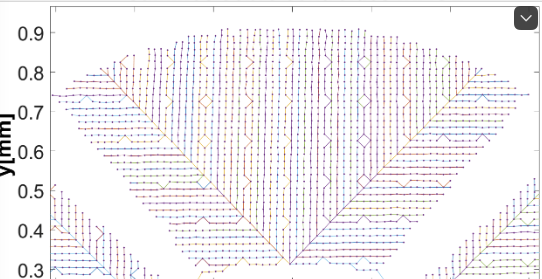
\includegraphics[width=0.85\linewidth]{cap4-caminos-ejemplo.png}
  \caption{Ejemplo de caminos de integración sobre un patrón densificado: cada trayectoria
  parte del punto de referencia y avanza de vecino en vecino hasta su destino. Tomada de
  un trabajo previo del autor \cite{ValderramaTesis2020}; el algoritmo es el mismo que se
  emplea aquí.}
  \label{fig:caminos-ejemplo}
\end{figure}

\subsection{Integración numérica por la regla del trapecio}\label{sec:trapecio}

Sobre cada camino se aplica la regla del trapecio a la integral de la Ec.~\ref{eq:integral-camino}. Para un camino $\bigl(r_0, r_1, \dots, r_p\bigr)$ con $r_i = (x_i, y_i)$ y aberración transversal $(T_x^{(i)}, T_y^{(i)})$ en cada nodo, la regla del trapecio entrega
\begin{equation}
W(r_p) = \sum_{i=0}^{p-1} \frac{1}{2f}\,\Bigl[\,(T_x^{(i)} + T_x^{(i+1)})(x_{i+1} - x_i) + (T_y^{(i)} + T_y^{(i+1)})(y_{i+1} - y_i)\,\Bigr],
\label{eq:trapecio_2}
\end{equation}
recordando que $W(r_0) = 0$ por la elección del punto de referencia. La operación es acumulativa: el frente de onda en cualquier nodo intermedio queda registrado en el momento en que se atraviesa, de modo que el algoritmo entrega simultáneamente $W$ en todas las microlentes del patrón densificado al recorrer el conjunto de caminos.

El producto final es la terna $(x_\ell, y_\ell, W)$ por microlente. Esta nube de puntos
describe el frente de onda reconstruido y constituye la entrada del análisis de resultados
del Capítulo~\ref{cap:resultados}.

\section{Comparación cuantitativa con la reconstrucción del fabricante}\label{sec:comparacion}

La comparación cuantitativa del método contra la reconstrucción del fabricante
(\textit{WFS Series Wavefront Analysis Software}, Thorlabs) se realiza sobre las mismas
mediciones: ambas reconstrucciones parten de los mismos centroides, quedan en el mismo
sistema de coordenadas y son directamente comparables. La métrica resultante es, por
construcción, relativa entre ambas reconstrucciones y no absoluta respecto a un frente de
onda teórico ideal. Esta elección es deliberada. El frente de onda bajo prueba lo genera
el espejo deformable con una fase ajustable pero no conocida en sentido absoluto
(Sección~\ref{sec:sistema-optico}). Determinarlo habría exigido colocar el sensor en el
plano conjugado del espejo y estudiar con más detalle el sistema de óptica adaptativa;
además, el método de corrimiento de puntos rota el sensor para cada dirección de barrido,
de modo que cada evaluación observa el frente de onda en un marco de referencia distinto,
y relacionar esos marcos requeriría conocer el centro físico del espejo y un análisis de
la rotación de frentes de onda —con las dificultades que presentan los polinomios de
Zernike en la frontera de la pupila— que queda fuera del alcance de este trabajo. Nada de
eso es necesario para validar el método: basta con que el frente de onda sea repetible
entre las capturas de una evaluación, y la comparación con el fabricante mide entonces
cuánto difieren dos reconstrucciones del mismo frente de onda obtenidas de las mismas
mediciones. La consistencia cualitativa del frente de onda reconstruido bajo distintas
configuraciones del espejo ofrece un criterio complementario de validez, y la
reconstrucción en vivo del software del fabricante que se muestra en el
Capítulo~\ref{cap:resultados} es sólo una referencia visual del estado del experimento. La
métrica adoptada es el valor cuadrático medio (RMS) de la diferencia entre ambos frentes
de onda, calculada después de eliminar el término global de inclinación que pueda quedar
entre ellos.

\subsection{Diferencia entre reconstrucciones}\label{sec:diferencia}

Sea $W(x,y)$ el frente de onda reconstruido por el método de corrimiento de puntos (Sección~\ref{sec:trapecio}) y $W_\text{TL}(x,y)$ el reconstruido por el software del fabricante para el mismo conjunto de mediciones; $W_\text{TL}$ se toma del archivo de mallado (\texttt{mesh}) que el software exporta junto con los centroides de la captura central (\texttt{d+0}), con las alturas evaluadas en los centros canónicos de microlente $(X_{TL},Y_{TL})$. Como los dos dominios de muestreo tienen densidades distintas (la lista densificada frente a la malla canónica del fabricante), la comparación punto a punto se realiza mediante un \emph{emparejamiento por vecino más cercano}: ambas reconstrucciones se restringen primero al mismo radio de selección $R$, y cada punto de una se empareja con el punto espacialmente más cercano de la otra (búsqueda de vecino más cercano, \texttt{knnsearch} en la implementación); las diferencias se evalúan sobre esos pares. La diferencia punto a punto es
\begin{equation}
\Delta W(x,y) = W(x,y) - W_\text{TL}(x,y).
\label{eq:diferencia-W}
\end{equation}
$\Delta W$ recoge dos contribuciones: errores locales propios del método de corrimiento de puntos (el residuo de interés) y un término global de inclinación. Este término no procede del frente de onda físico —es el mismo frente de onda, medido con el mismo sensor— sino de la referencia de fase plana que adopta cada reconstrucción: la integración por la regla del trapecio (Sección~\ref{sec:trapecio}) parte de $W(r_0)=0$ y recupera el frente de onda salvo una constante de pistón, sin fijar su inclinación absoluta, mientras que el ajuste modal del fabricante fija la suya con su propio criterio. Una inclinación residual del plano del sensor respecto al haz, en cambio, afecta por igual a ambas reconstrucciones y no genera inclinación relativa entre ellas. Como estos \textit{tip} y \textit{tilt} aparentes no contienen información sobre la calidad del método, el término debe removerse antes de cuantificar el residuo.

\subsection{Eliminación de \textit{tip} y \textit{tilt} por ajuste de plano}\label{sec:tip-tilt}

Para aislar el residuo local, a cada una de las dos reconstrucciones se le ajusta por mínimos cuadrados, sobre los puntos de su propio dominio, un plano que captura su inclinación y su desplazamiento vertical residuales:
\begin{equation}
W(x,y) \approx a\,x + b\,y + c, \qquad W_\text{TL}(x,y) \approx a_\text{TL}\,x + b_\text{TL}\,y + c_\text{TL},
\label{eq:plano-ajuste}
\end{equation}
donde en cada caso los coeficientes $a$ y $b$ corresponden a las pendientes residuales (\textit{tip} y \textit{tilt}) y el término constante $c$ absorbe el pistón. Nótese que $a$ y $b$ son pendientes, es decir, cocientes de longitud entre longitud (mm/mm), y por tanto adimensionales, mientras que $c$ tiene unidades de longitud (mm); en lo sucesivo, los coeficientes de plano se reportan sin repetir estas unidades. Cada frente de onda se corrige restándole su propio plano, y la diferencia entre los frentes de onda así corregidos, evaluada sobre los pares del emparejamiento (Sección~\ref{sec:diferencia}), es
\begin{equation}
\Delta W'(x,y) = \bigl[W(x,y) - (a\,x + b\,y + c)\bigr] - \bigl[W_\text{TL}(x,y) - (a_\text{TL}\,x + b_\text{TL}\,y + c_\text{TL})\bigr].
\label{eq:residuo}
\end{equation}
$\Delta W'$ representa la discrepancia entre las dos reconstrucciones una vez removida la inclinación global de cada una, y es la magnitud físicamente relevante para juzgar la fidelidad del método. Los coeficientes de ambos planos se reportan en las tablas resumen de cada evaluación del Capítulo~\ref{cap:resultados}.

\subsection{Indicador escalar (RMS)}\label{sec:rms}

El indicador final de fidelidad es el RMS del residuo sobre las $N$ microlentes incluidas en la región útil (Sección~\ref{sec:seleccion-region}):
\begin{equation}
\text{RMS} = \sqrt{\frac{1}{N} \sum_{i=1}^{N} \bigl[\Delta W'_i\bigr]^2}.
\label{eq:rms}
\end{equation}
Este valor es el que se reporta como métrica cuantitativa de la comparación en cada una de las evaluaciones del Capítulo~\ref{cap:resultados}. Hay que subrayar que, en una evaluación con aberración impuesta no nula, el RMS de un frente de onda individual describe la magnitud de la aberración bajo prueba, no la calidad del método; la fidelidad solo queda definida al comparar contra una referencia, y por ello la métrica reportada es siempre el RMS de la \emph{diferencia} entre reconstrucciones. El procedimiento, junto con el tratamiento adicional descrito en la Sección~\ref{sec:segundo-tratamiento} cuando es aplicable, constituye la cadena completa de comparación cuantitativa empleada en este trabajo.

\subsection{Tratamiento del pistón residual entre reconstrucciones sobre dominios asimétricos}\label{sec:segundo-tratamiento}

El procedimiento de remoción de tip, tilt y pistón descrito en la
Sección~\ref{sec:tip-tilt} se aplica de manera estándar a cada una de las dos
reconstrucciones por separado, ajustando un plano de mejor ajuste por mínimos cuadrados a
su propio dominio. Cuando los dos dominios coinciden en densidad de muestreo, los planos
individuales se compatibilizan de forma natural y la diferencia residual queda libre de
modos lineales globales. Sin embargo, cuando los dos dominios difieren sustancialmente en
densidad (situación habitual al comparar la lista densificada producida por el método de
corrimiento de puntos contra el mallado canónico que entrega el software del fabricante)
los planos por mínimos cuadrados se ajustan ponderando de forma desigual las regiones de
la pupila donde cada método tiene más muestras, pudiendo dejar un offset relativo entre
las dos superficies residuales que no proviene del frente de onda físico bajo prueba sino
del propio procedimiento de remoción de modos bajos.

Para corregir este sesgo se aplica un segundo tratamiento directamente sobre la diferencia. El tratamiento se aplica en todas las evaluaciones; su efecto es apreciable cuando los dominios de ambas reconstrucciones difieren y la aberración tiene media no nula sobre el disco, como la esférica $Z_{13}$ (evaluaciones 2 y 3), y resulta nulo cuando la media angular de la aberración se anula para cualquier radio, como en el tetrafoil $Z_{11}$ (evaluación 1), porque entonces el pistón relativo entre dominios distintos desaparece por simetría. La idea es la siguiente: si después de la remoción individual de TTP la diferencia $\Delta W'$ aún contiene un plano residual $a'x + b'y + c'$ (tip, tilt y pistón \emph{relativos} entre las dos reconstrucciones), ese plano no proviene del frente de onda físico (ambas reconstrucciones miden el mismo frente de onda) sino del propio procedimiento de remoción, y debe eliminarse antes de calcular la métrica. Para ello se ajusta por mínimos cuadrados un único plano a $\Delta W'$ sobre el conjunto de puntos emparejados y se le resta:
\begin{equation}
\Delta W''(x,y) = \Delta W'(x,y) - (a'\,x + b'\,y + c'),
\label{eq:residuo-doble}
\end{equation}
y el RMS final de fidelidad se calcula sobre $\Delta W''$ con la misma expresión de la Ec.~\ref{eq:rms}. Dos propiedades sostienen este procedimiento. Primero, es algebraicamente equivalente a corregir cualquiera de los dos frentes de onda con ese mismo plano, pues $\Delta W' - P = (W' - P) - W'_\text{TL}$. Segundo, el resultado no depende del orden de las operaciones: como todos los términos removidos son planos, ajustar y restar un plano a la diferencia al final elimina por completo la componente plana de $\Delta W$, cualesquiera hayan sido los planos restados antes a cada frente de onda por separado. En los casos en que los dominios de muestreo son compatibles, los coeficientes $(a', b', c')$ resultan despreciables y el segundo tratamiento no altera la métrica, como se verifica en el Capítulo~\ref{cap:resultados}.

\chapter{Resultados}\label{cap:resultados}

En este capítulo se presentan las tres evaluaciones experimentales realizadas con el
arreglo descrito en el Capítulo~\ref{cap:metodologia}, correspondientes a las superficies
caracterizadas en el alcance del presente trabajo. Cada evaluación combina una dirección
de barrido $(m,n)$ con una configuración del espejo deformable, y produce un conjunto de
centroides corridos sobre el cual se aplica la metodología de las
Secciones~\ref{sec:cent-a-aberracion}--\ref{sec:rms}: composición de los $\varepsilon$
corrimientos, selección de la región útil, integración numérica por la regla del trapecio,
eliminación de \textit{tip} y \textit{tilt} por ajuste de plano, y comparación
cuantitativa basada en el RMS de las diferencias calculadas punto a punto contra la
reconstrucción reportada por el software del fabricante, como se describió en el capítulo
anterior (Secciones~\ref{sec:diferencia}--\ref{sec:rms}). La primera evaluación se
documenta paso a paso para fijar el procedimiento; las dos restantes condensan los pasos
repetidos.

Antes de describir las evaluaciones hay que precisar la convención de notación que se
emplea en este capítulo. Cuando en este capítulo se hace referencia a una ``aberración
impuesta $Z_{11}$'' o ``aberración impuesta $Z_{13}$'' se designa el modo del software de
control del espejo deformable que fue activado para generar el frente de onda bajo prueba
(Sección~\ref{sec:control-adquisicion}); estas etiquetas identifican la configuración
experimental del espejo, no coeficientes Zernike obtenidos por descomposición posterior de
la reconstrucción. El método de corrimiento de puntos aquí desarrollado entrega la
reconstrucción como una nube de puntos $(x_l,\,y_l,\,W)$ y no incluye un ajuste modal
sobre el frente de onda reconstruido; por tanto, en este trabajo no se reportan
coeficientes Zernike calculados a partir de los datos. La razón es de alcance, no de
incompatibilidad: lo que se propone es el muestreo denso y su integración directa por la
regla del trapecio, la forma más simple de reconstruir a partir de los puntos; sobre la
misma lista densificada podría aplicarse cualquier otro método de integración, incluido un
ajuste modal, y hacerlo queda fuera de la extensión de este trabajo. La descomposición
Zernike que el software del fabricante muestra en las capturas de la interfaz en vivo se
incluye en las figuras de estado experimental únicamente como referencia del setup, sin
entrar en el análisis cuantitativo. La convención de índices de Zernike empleada por el
software y las formas analíticas de los modos evaluados quedaron establecidas en la
Sección~\ref{sec:convencion-zernike} (Tabla~\ref{tab:modos-dm}).

\section[Primera evaluación: dirección (m,n)=(1,2), aberración Z11 negativa]{Primera evaluación: dirección \mbox{$(m,n)=(1,2)$}, aberración $Z_{11}$ negativa}\label{sec:eval-z11-m1n2}

\begin{figure}[htbp]
  \centering
  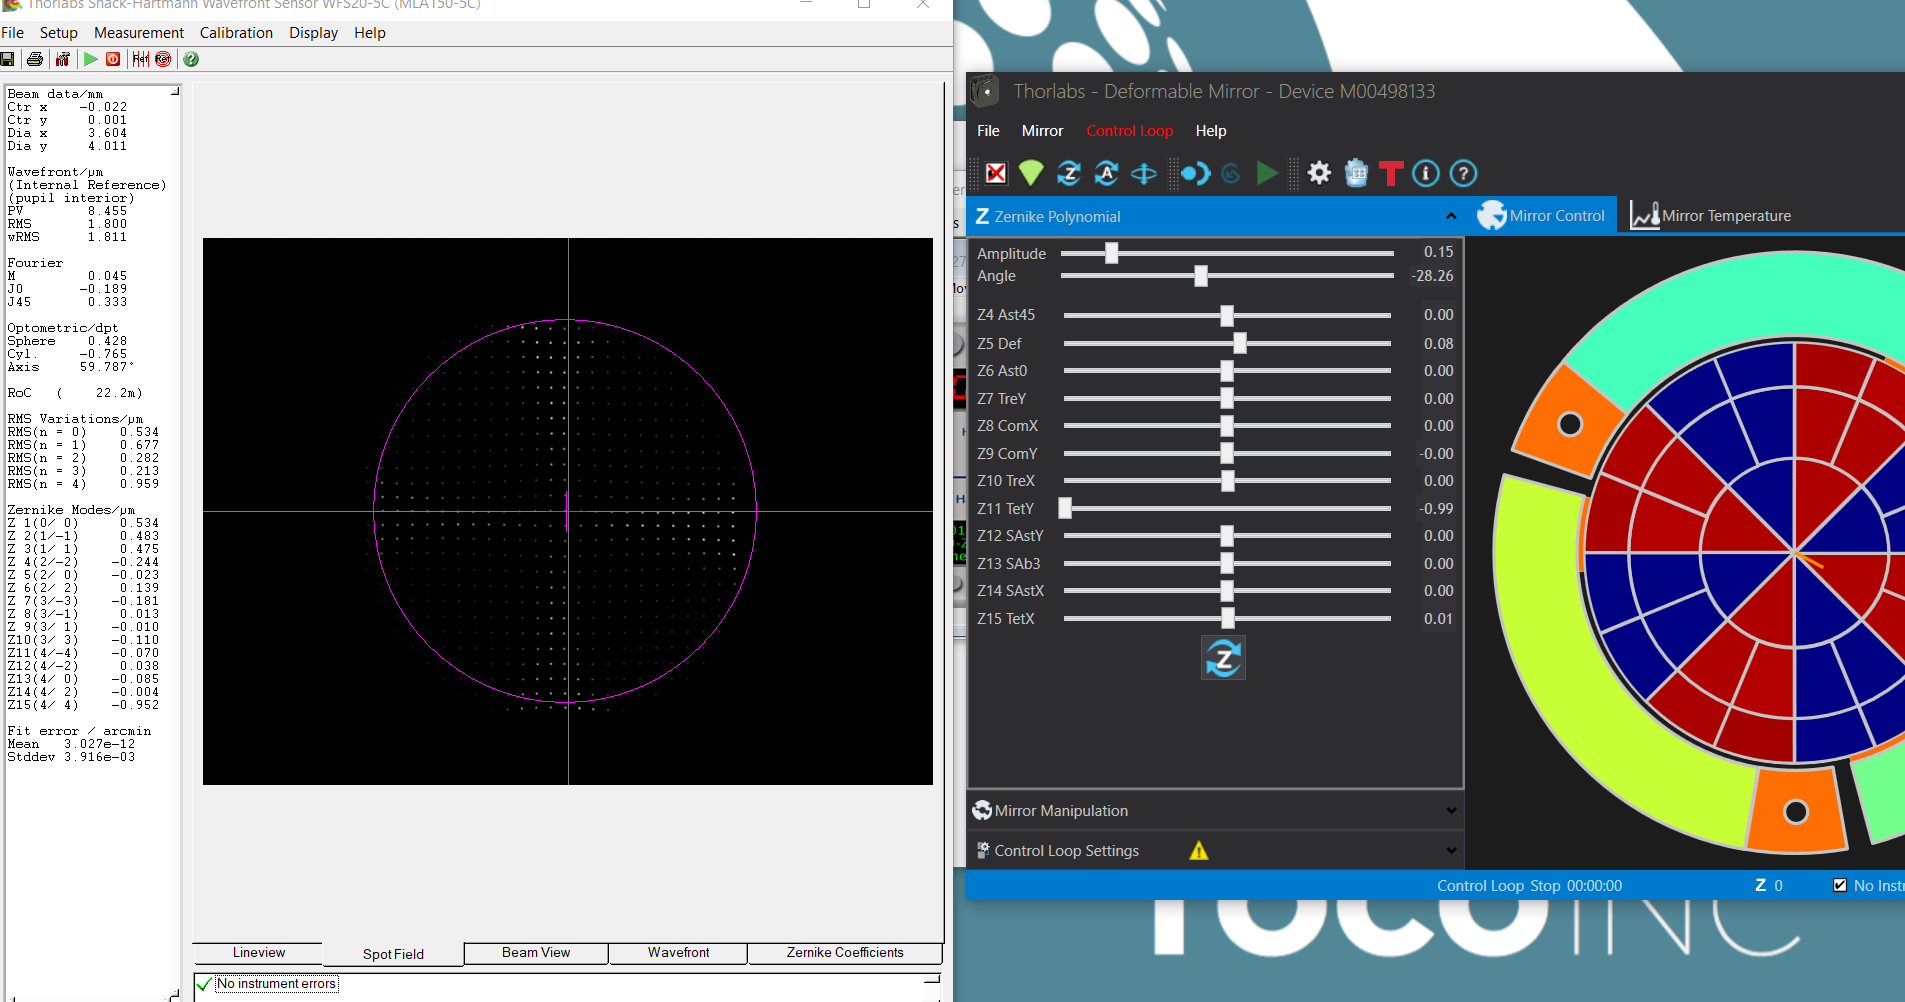
\includegraphics[width=0.95\linewidth]{cap5-fig5_0-setup-inicial-thorlabs.png}
  \caption{Estado inicial del experimento para la primera evaluación, capturado desde la
  interfaz en vivo del software del fabricante (\textit{WFS Series Wavefront Analysis
  Software}, Thorlabs) en la posición central del barrido ($\sigma=0$, sin corrimiento) y
  con el espejo deformable configurado en el modo $Z_{11}$ (tetrafoil,
  Tabla~\ref{tab:modos-dm}) con el deslizador de amplitud del software en $-0.99$. La
  captura muestra simultáneamente el shack-hartmanngrama, la reconstrucción del frente de
  onda y los coeficientes de Zernike reportados por el software. Esta figura se incluye
  como referencia del estado experimental; no se utiliza en el análisis cuantitativo
  posterior. Los datos del shack-hartmanngrama (panel izquierdo de la captura) son
  procesados por el software de Thorlabs; de ese procesamiento se obtienen los centroides
  canónicos que se muestran en el panel izquierdo de la Fig.~\ref{fig:cap5-fig5-1-1}.}
  \label{fig:cap5-fig5-0}
\end{figure}

La primera evaluación corresponde a la dirección de barrido $(m,n)=(1,2)$, para la cual el
factor de densificación es $\varepsilon = m^2 + n^2 = 5$. El espejo deformable se
configura para imponer el modo $Z_{11}$ (tetrafoil, Tabla~\ref{tab:modos-dm}) en amplitud
negativa, con el deslizador del software en $-0.99$ dentro de su intervalo $[-1,+1]$, de
modo que el frente de onda incidente sobre la matriz de microlentes sea repetible aunque
no de magnitud absoluta conocida (véase Sección~\ref{sec:sistema-optico}). Para esta
configuración se registran cinco spotgramas (los patrones de puntos del sensor, como los
Shack-Hartmanngramas de la Fig.~\ref{fig:shg-crudo}), correspondientes a los
desplazamientos acumulados $\sigma_i \in
\{-0.1342,\allowbreak\,-0.0671,\allowbreak\,0,\allowbreak\,+0.0671,\allowbreak\,+0.1342\}$~mm
(múltiplos del paso $\sigma = 0.0671$~mm de la Ec.~\ref{eq:distdesp}) a lo largo de la
dirección $(1,2)$.

Como punto de partida, la Fig.~\ref{fig:cap5-fig5-0} documenta el estado del sistema
previo a la adquisición. La captura corresponde a la interfaz en vivo del software del
fabricante (\textit{WFS Series Wavefront Analysis Software}, Thorlabs) en la posición
central $\sigma=0$, con el haz alineado y el espejo deformable configurado en $Z_{11}$ con
amplitud $-0.99$. El software entrega simultáneamente el shack-hartmanngrama, la
reconstrucción del frente de onda y la descomposición en coeficientes de Zernike. Esta
visualización no se utiliza en el análisis cuantitativo posterior, pero sirve como
referencia del estado experimental sobre el que se realiza la evaluación.

\subsection{Datos en crudo: centroides corridos y referencia del fabricante}\label{sec:z11-datos-crudos}

El primer producto experimental son los conjuntos de centroides extraídos de los cinco
spotgramas. La Fig.~\ref{fig:cap5-fig5-1-1} superpone, sobre el plano del sensor, dos
conjuntos de puntos obtenidos del mismo experimento físico pero tratados de forma
distinta: en color, los centroides corridos resultantes de aplicar la composición de la
Sección~\ref{sec:composicion-corrimientos} a los cinco spotgramas (lista densificada de
$\varepsilon$ veces más muestras); en negro, los centroides de la toma central $\sigma=0$
tal como los entrega el software de Thorlabs (en adelante, los puntos \emph{canónicos}; es
decir, los del arreglo original sin densificar), que constituyen la referencia con la que
se contrastará la reconstrucción al final de la sección. Esta superposición ilustra dos
observaciones que sostienen el resto del análisis: primero, que ambos conjuntos provienen
de la misma adquisición y comparten los puntos de la toma central, lo que garantiza que la
comparación final no recae sobre experimentos distintos sino sobre dos estrategias de
muestreo aplicadas al mismo frente de onda; segundo, que el corrimiento de puntos
multiplica por $\varepsilon = 5$ el número de muestras (reduciendo el paso efectivo entre
puntos en un factor $\sqrt{\varepsilon}$) sin necesidad de modificar la geometría del
arreglo de microlentes, condición indispensable para preservar el rango dinámico angular
del sensor (Ec.~\ref{eq:alphamax}).

\begin{figure}[htbp]
  \centering
  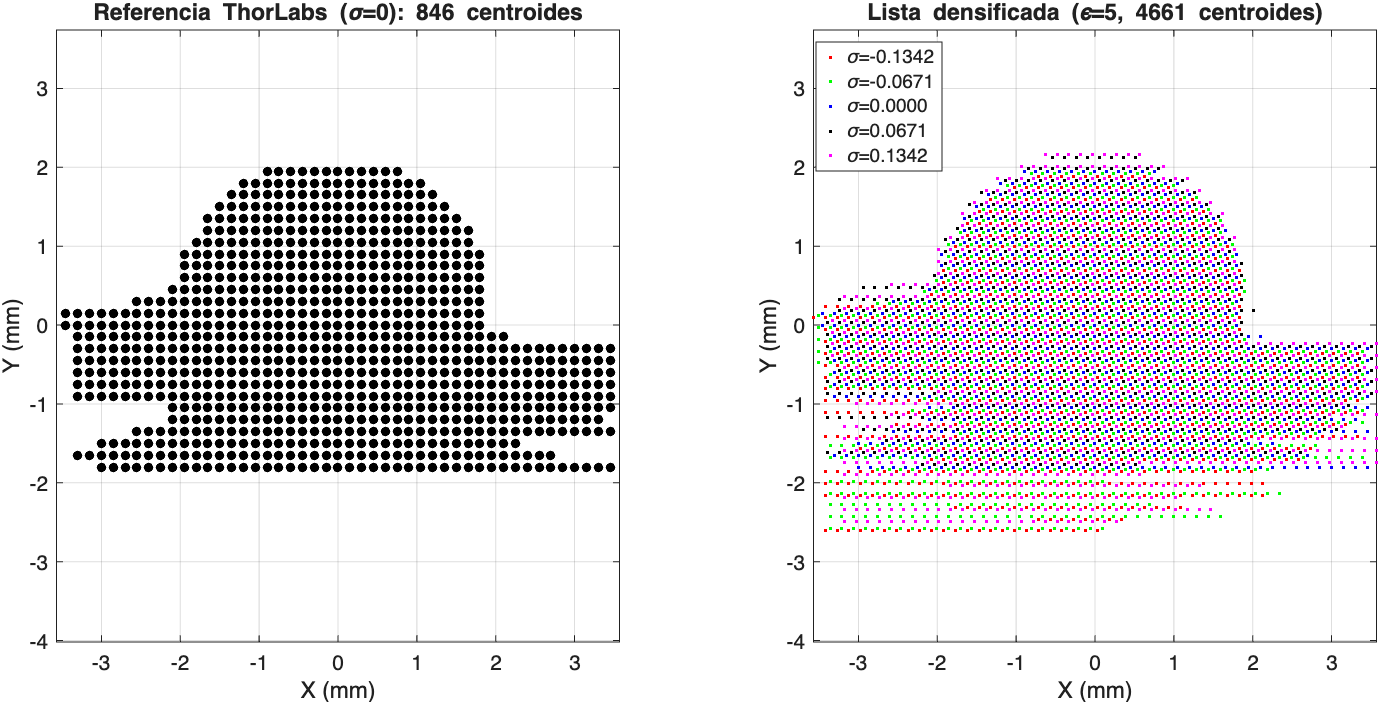
\includegraphics[width=0.95\linewidth]{cap5-fig5_1_1-thorlabs-vs-densificada.png}
  \caption{Centroides extraídos del experimento de la primera evaluación, presentados
  sobre el plano del sensor. \textbf{Izquierda}: centroides de la toma central $\sigma=0$
  tal como los entrega el software de Thorlabs, que constituyen la referencia con la que
  se contrastará la reconstrucción al final de la sección. \textbf{Derecha}: lista
  densificada de centroides corridos correspondiente a los cinco spotgramas tras aplicar
  la composición de la Sección~\ref{sec:composicion-corrimientos} ($\varepsilon=5$), con
  cada conjunto coloreado según su desplazamiento $\sigma_i$. Ambos conjuntos provienen
  del mismo experimento físico. Conviene señalar que los ejes coordenados $x$-$y$ de esta
  figura, en el plano transversal a la dirección de propagación, están rotados un ángulo
  $\theta$ respecto al sistema coordenado del espejo deformable que genera los modos de
  Zernike (Sección~\ref{sec:convencion-zernike}).}
  \label{fig:cap5-fig5-1-1}
\end{figure}

\subsection{Acercamiento a la lista densificada}\label{sec:z11-acercamiento}

A la escala de la Fig.~\ref{fig:cap5-fig5-1-1} la separación entre puntos vecinos no es
discernible visualmente, lo que dificulta apreciar el efecto de densificación introducido
por el método. La Fig.~\ref{fig:cap5-fig5-1-2} muestra un recorte de la misma lista
densificada sobre una subregión del campo del sensor: en ella se distinguen los grupos de
$\varepsilon=5$ centroides que aporta cada microlente y la geometría con la que el
corrimiento $(m,n)=(1,2)$ los distribuye dentro de cada celda. El recorte sirve como
evidencia visual de que el aumento de muestreo se obtiene sin alterar la geometría física
del arreglo de microlentes.

\begin{figure}[htbp]
  \centering
  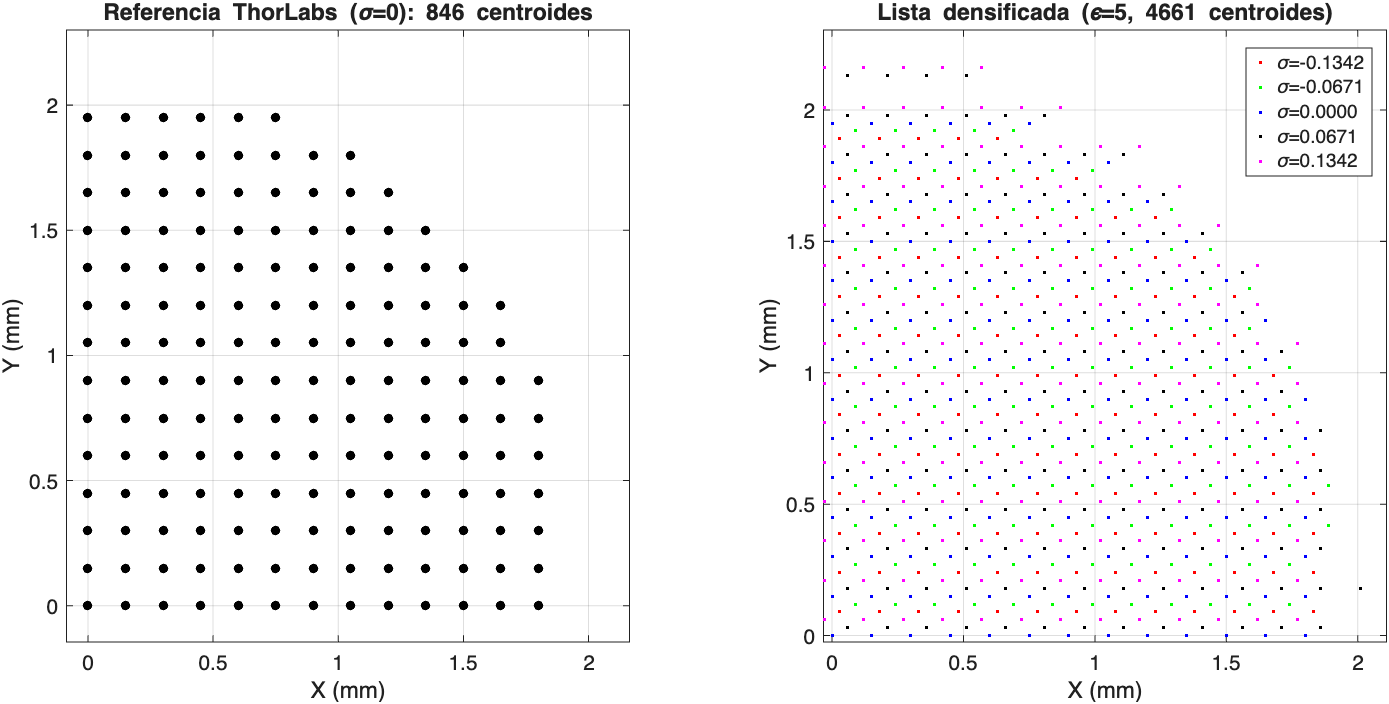
\includegraphics[width=0.85\linewidth]{cap5-fig5_1_2-densificada-zoom.png}
  \caption{Acercamiento a una subregión de la lista densificada de la
  Fig.~\ref{fig:cap5-fig5-1-1}. Cada celda de microlente aporta $\varepsilon=5$ centroides
  distribuidos a lo largo de la dirección $(m,n)=(1,2)$ por efecto del corrimiento
  controlado del haz.}
  \label{fig:cap5-fig5-1-2}
\end{figure}

\subsection{Selección de la región útil}\label{sec:z11-seleccion}

La lista densificada de la Fig.~\ref{fig:cap5-fig5-1-1} no es directamente integrable:
contiene microlentes cuyo centroide no pudo extraerse en alguna de las cinco tomas
(registrados como \texttt{NaN} al componer la lista) y, hacia los bordes del campo
iluminado, regiones donde los puntos válidos quedan desconectados de la nube central.
Ambos efectos son problemáticos para la reconstrucción por integración numérica descrita
en la Sección~\ref{sec:integracion}: las trayectorias voraces sobre las que se aplica la
regla del trapecio requieren conectividad entre vecinos válidos, y un punto aislado o un
\texttt{NaN} interrumpen el camino y propagan la inconsistencia al resto de la malla.

Por esta razón se recorta la lista a una región circular centrada en el campo del sensor,
siguiendo el procedimiento definido en la Sección~\ref{sec:seleccion-region} del
Capítulo~\ref{cap:metodologia}. La elección de una región circular no es arbitraria, ya
que respeta la simetría natural del frente de onda incidente, garantiza la conectividad de
la nube de puntos sobre la que se realiza la integración, y permite descartar de forma
uniforme las celdas con datos faltantes en los bordes sin sesgar direccionalmente el
resultado. El radio se fija de modo que la región resultante quede contenida dentro de la
zona donde los cinco spotgramas reportan centroides válidos. La Fig.~\ref{fig:cap5-fig5-2}
muestra la lista densificada de centroides antes y después de aplicar esta selección,
junto con la frontera circular utilizada como criterio. Hay que precisar que los puntos
graficados son centroides, es decir, las posiciones de las manchas de luz registradas en
la cámara, no los centros geométricos de las microlentes; estos últimos son posiciones
matemáticas conocidas \textit{a priori} y no aparecen en la figura.

\begin{figure}[htbp]
  \centering
  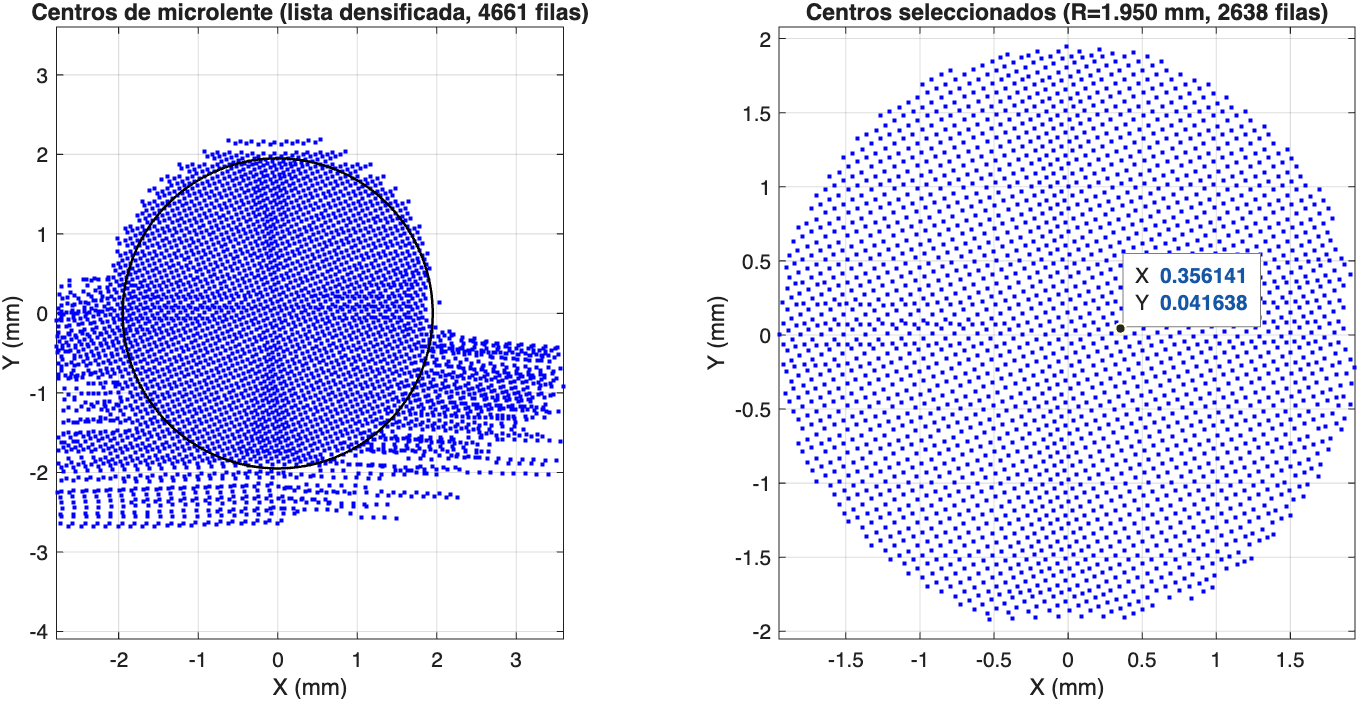
\includegraphics[width=0.95\linewidth]{cap5-fig5_2-region-seleccionada.png}
  \caption{Selección de la región útil sobre la lista densificada de centroides.
  \textbf{Izquierda}: lista completa con la frontera circular de radio $R$ superpuesta
  como criterio de selección. \textbf{Derecha}: centroides sobrevivientes tras descartar
  las celdas cuyo dato cae fuera del círculo o no pudo extraerse en alguna toma. Los
  puntos graficados son centroides (manchas de luz en la cámara); la selección define qué
  celdas de microlente contribuyen a la integración numérica descrita en la
  Sección~\ref{sec:integracion}.}
  \label{fig:cap5-fig5-2}
\end{figure}

\subsection{Centros, centroides y caminos de integración}\label{sec:z11-caminos}

Una vez fijada la región útil, la lista densificada queda definida por dos conjuntos de
puntos sobre el plano del sensor que hay que distinguir explícitamente antes de proceder a
la integración. Por un lado, los \emph{centros de microlente} $(x_l,\,y_l)$ son las
posiciones matemáticas de los vértices del arreglo de microlentes, conocidas \textit{a
priori} a partir de la geometría del sensor (paso $0.150$~mm); por el otro, los
\emph{centroides} $(x_c,\,y_c)$ son las posiciones medidas de las manchas de luz que cada
microlente forma sobre la cámara. La diferencia $(T_x, T_y) = (x_l - x_c,\, y_l - y_c)$
entre ambos en una misma celda codifica la pendiente local del frente de onda incidente
sobre esa microlente, y es la cantidad sobre la que opera el integrador de la
Sección~\ref{sec:integracion}. La Fig.~\ref{fig:cap5-fig5-3}\,a) presenta ambos conjuntos
superpuestos sobre la región seleccionada: la separación visible entre cada par de puntos
es la manifestación gráfica de la deflexión transversal que produce la aberración impuesta
por el espejo deformable.

\begin{figure}[htbp]
  \centering
  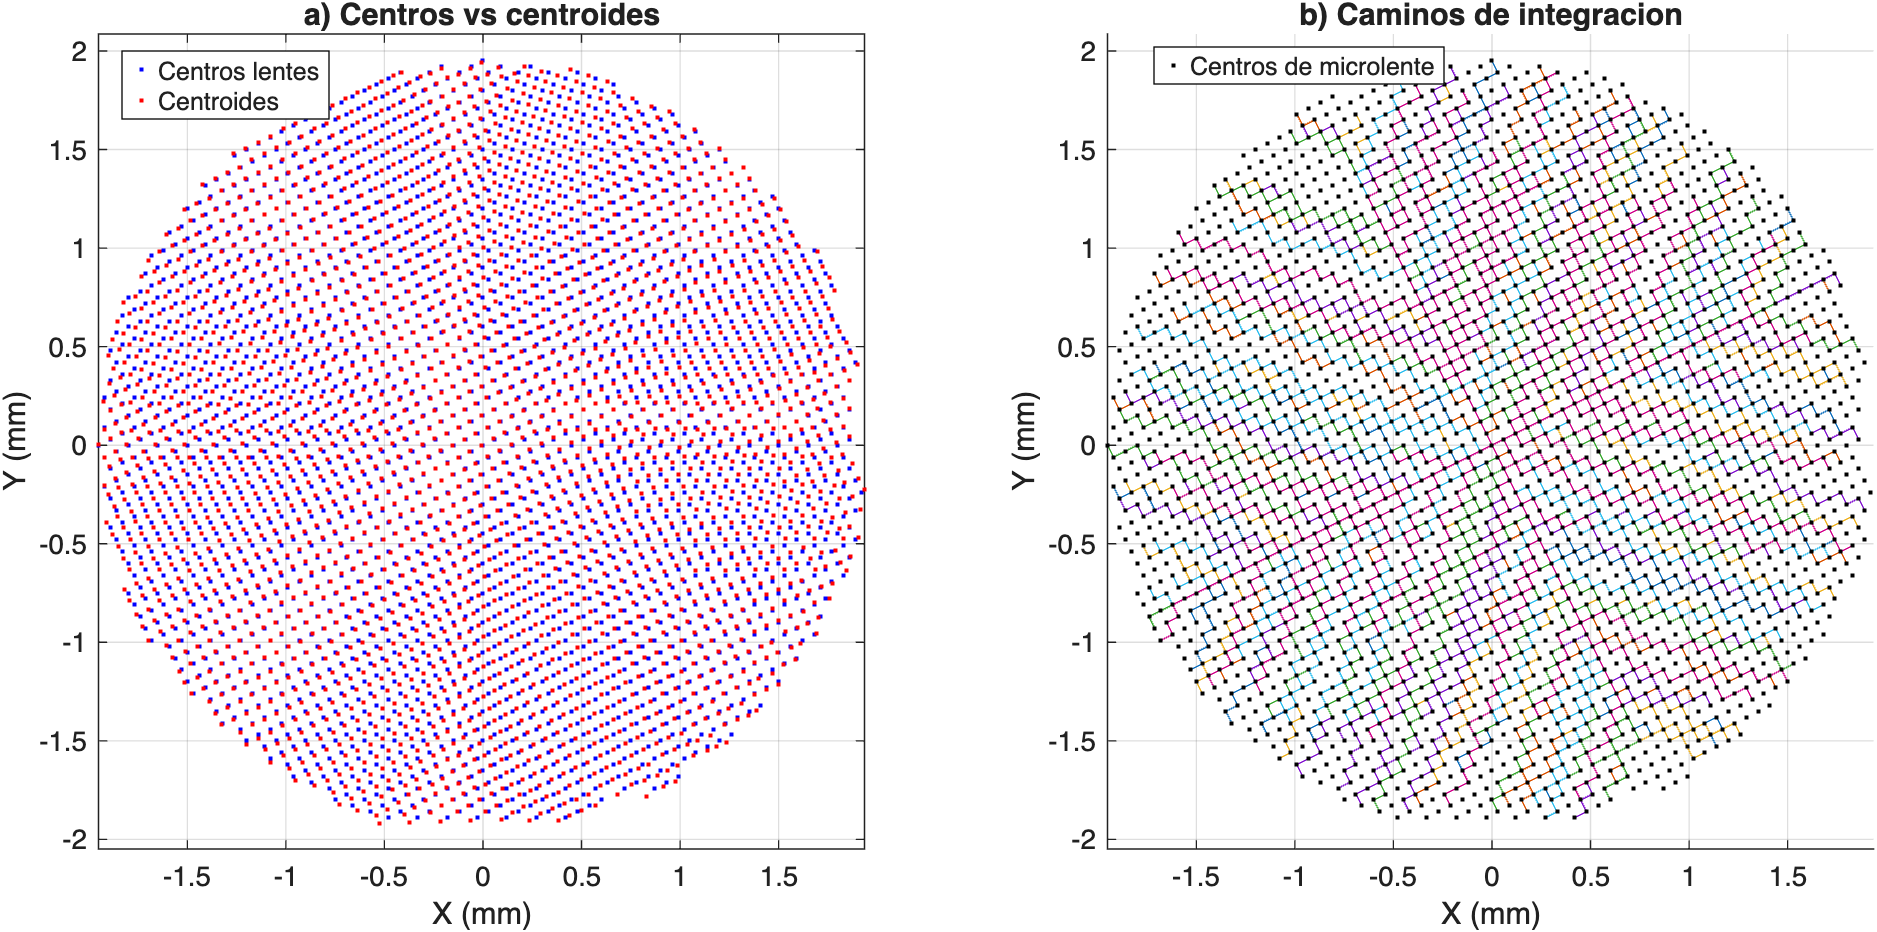
\includegraphics[width=\linewidth]{cap5-centros-centroides-caminos.png}
  \caption{Estructura geométrica utilizada por la integración numérica sobre la región
  seleccionada. \textbf{a)} Centros de microlente $(x_l,\,y_l)$ (azul) y centroides
  medidos $(x_c,\,y_c)$ (rojo) superpuestos; la separación dentro de cada celda codifica
  la pendiente local del frente de onda. \textbf{b)} Caminos de integración depurados
  (cada uno en un color, con paleta cíclica de siete colores) trazados sobre los centros
  de microlente; por legibilidad se muestra una de cada tres trayectorias, aunque la
  integración utiliza el conjunto completo.}
  \label{fig:cap5-fig5-3}
\end{figure}

Sobre los centros de microlente se construyen las trayectorias de integración requeridas
por la regla del trapecio. La función \texttt{intpath} genera, para cada punto de la
región seleccionada, una secuencia voraz de vecinos contiguos que parte del centro
geométrico de la nube y avanza hasta el punto destino, usando como umbral de vecindad la
cota $h = P_L\sqrt{2}/\sqrt{m^2+n^2}$ definida en la Sección~\ref{sec:caminos-integracion}
(Ec.~\ref{eq:cota-vecinas}). Las trayectorias así generadas se depuran eliminando las
redundantes, como se describe en la Sección~\ref{sec:caminos-integracion}. La
Fig.~\ref{fig:cap5-fig5-3}\,b) ilustra el resultado: cada camino se traza en un color
distinto (paleta cíclica de siete colores) y, para no saturar la figura, se muestra una de
cada tres trayectorias depuradas; la integración numérica posterior, sin embargo, utiliza
el conjunto completo. Estos caminos son los que alimentan la regla del trapecio para
producir el frente de onda reconstruido que se presenta en la siguiente subsección.

\subsection{Reconstrucción inicial del frente de onda}\label{sec:z11-reconstruccion-inicial}

\begin{figure}[htbp]
  \centering
  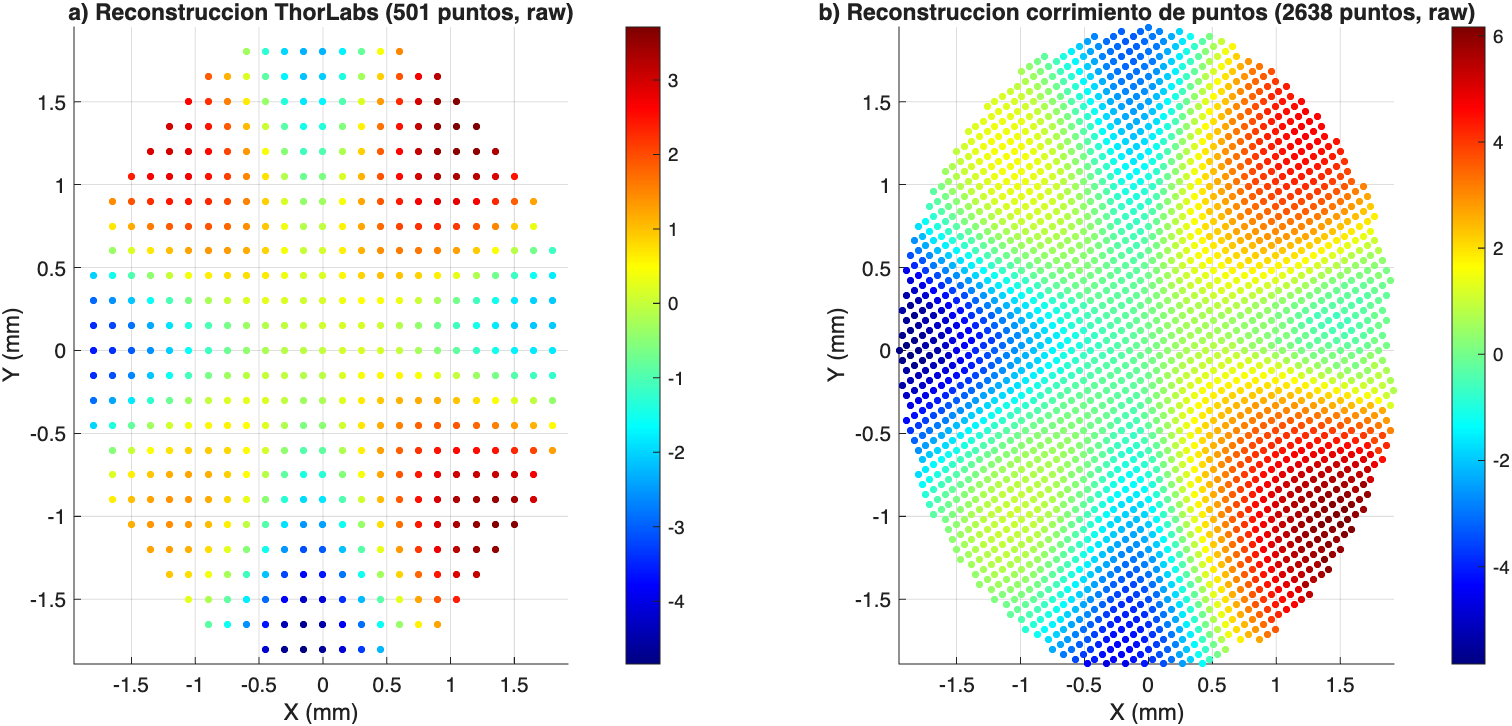
\includegraphics[width=\linewidth]{cap5-fig5_4_2-reconstruccion-mapa-colores.png}
  \caption{Reconstrucción inicial del frente de onda en vista cenital, ambas previas a
  cualquier remoción de modos bajos. \textbf{a)} Reconstrucción de Thorlabs
  $(X_{TL},Y_{TL},Z_{TL})$ sobre la malla canónica de microlentes (501 puntos).
  \textbf{b)} Reconstrucción por el método de corrimiento de puntos $(x_l,y_l,W)$ sobre la
  lista densificada (2638 puntos). El color codifica la altura del frente de onda; la
  diferencia de densidad entre paneles es el efecto del factor $\varepsilon=5$.}
  \label{fig:cap5-fig5-4-2}
\end{figure}

Aplicando la regla del trapecio a lo largo de los caminos de integración de la
Fig.~\ref{fig:cap5-fig5-3}\,b) sobre los pares $(T_x,T_y)$ asociados a cada microlente, se
obtiene el frente de onda $W(x_l,y_l)$ reconstruido por el método de corrimiento de
puntos. Para juzgar la calidad de la reconstrucción, no basta con mirarla en aislado: hay
que confrontarla contra el frente de onda que entrega el software de Thorlabs sobre las
mismas mediciones, calculado por su propio algoritmo de reconstrucción modal y reportado
como un mallado de alturas. La Fig.~\ref{fig:cap5-fig5-4-2} presenta ambas
reconstrucciones en vista cenital, con el color codificando la altura del frente de onda
en cada centro de microlente; la disposición lado a lado deja en evidencia tanto la
estructura espacial común a ambas reconstrucciones como el aumento de densidad de muestreo
que aporta el corrimiento de puntos respecto al mallado canónico del fabricante.

La vista cenital es útil para apreciar la densidad y el patrón de iluminación, pero pierde
la magnitud relativa entre regiones del frente de onda. La Fig.~\ref{fig:cap5-fig5-4-1}
muestra las mismas dos reconstrucciones en perspectiva tridimensional, con el eje $z$
ahora explícito en micrómetros.

\begin{figure}[htbp]
  \centering
  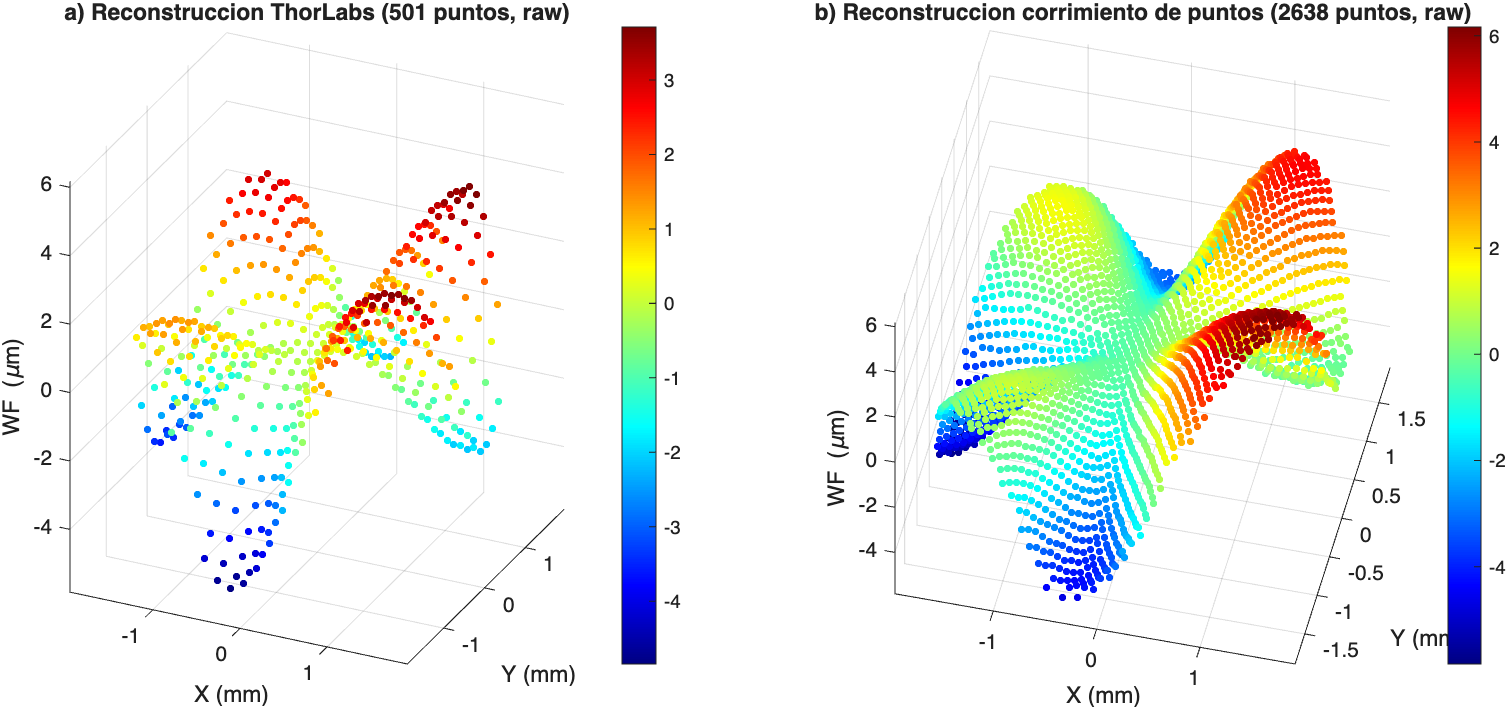
\includegraphics[width=\linewidth]{cap5-fig5_4_1-reconstruccion-perspectiva.png}
  \caption{Reconstrucción inicial del frente de onda en perspectiva tridimensional, ambas
  previas a la remoción de tip, tilt y pistón. \textbf{a)} Reconstrucción de Thorlabs.
  \textbf{b)} Reconstrucción por el método de corrimiento de puntos. El eje $z$ se reporta
  en micrómetros para mejor lectura. La inclinación global visible en ambas nubes
  corresponde a tip y tilt residuales del montaje y de la integración (recuperación salvo
  una constante de pistón), no a la aberración impuesta por el espejo deformable; su
  efecto sobre la diferencia entre reconstrucciones se discute en el cuerpo del texto.}
  \label{fig:cap5-fig5-4-1}
\end{figure}

En esta vista se hace evidente que ambas reconstrucciones, además de la curvatura asociada
a la aberración impuesta por el espejo deformable, presentan una inclinación global
aparente: las dos nubes de puntos no descansan sobre un plano horizontal sino sobre planos
ligeramente inclinados. Esta inclinación no es una propiedad del frente de onda físico
bajo prueba, sino tip y tilt residuales que cada método arrastra de la cadena de medición
y de la propia integración (que recupera el frente de onda salvo una constante de pistón).
El RMS de la diferencia punto a punto entre ambas reconstrucciones, calculado en esta
etapa previa al procesado mediante el emparejamiento por vecino más cercano descrito en la
Sección~\ref{sec:diferencia}, resulta de $1.16~\mu$m. Este valor es marcadamente mayor que
la magnitud típica de los residuos esperables del método y refleja, en su mayor parte, la
diferencia de tip, tilt y pistón entre las dos reconstrucciones más que el residuo real de
interés. Es por esta razón que, antes de cuantificar la fidelidad del método, se remueven
tip, tilt y pistón sobre ambos frentes de onda según el procedimiento de la
Sección~\ref{sec:tip-tilt}; el resultado se presenta en la siguiente subsección.

\subsection{Reconstrucción tras la remoción de tip, tilt y pistón}\label{sec:z11-reconstruccion-sin-ttp}

\begin{figure}[htbp]
  \centering
  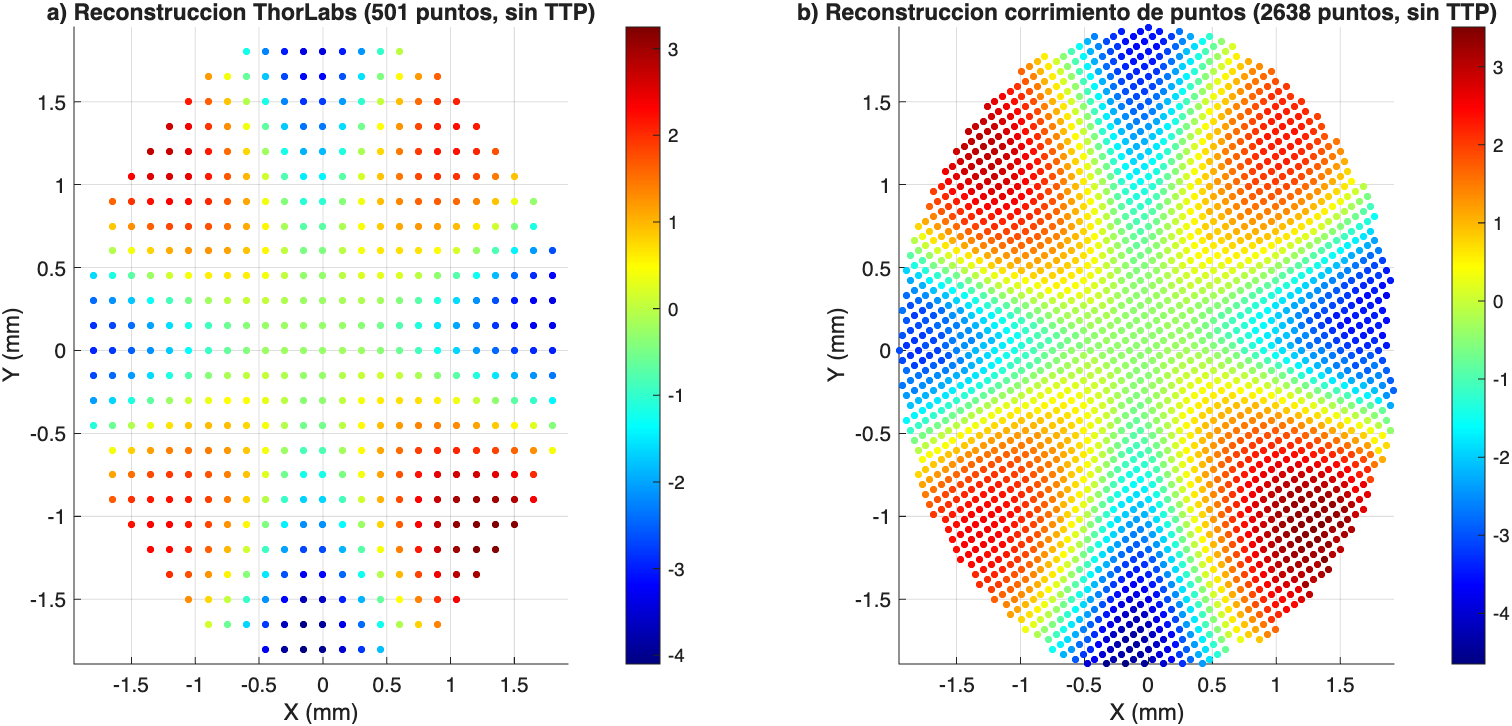
\includegraphics[width=\linewidth]{cap5-fig5_5_1-reconstruccion-sin-ttp-mapa.png}
  \caption{Reconstrucción del frente de onda en vista cenital tras la remoción de tip,
  tilt y pistón. \textbf{a)} Reconstrucción de Thorlabs (501 puntos). \textbf{b)}
  Reconstrucción por el método de corrimiento de puntos (2638 puntos). El color codifica
  la altura del frente de onda residual; la escala es ahora consistente con la magnitud de
  la aberración impuesta y permite comparar la estructura espacial de ambos frentes de
  onda en igualdad de condiciones.}
  \label{fig:cap5-fig5-5-1}
\end{figure}

A cada uno de los dos frentes de onda reconstruidos se le ajusta, por mínimos cuadrados
sobre los puntos de su propio dominio, un plano de la forma $z = aX + bY + c$ que captura
la inclinación global y el desplazamiento vertical residuales
(Sección~\ref{sec:tip-tilt}). Los coeficientes $(a, b, c)$ son las dos pendientes y el
pistón definidos en la Sección~\ref{sec:tip-tilt} (las pendientes son adimensionales y $c$
se da en mm). Para esta evaluación los planos restados son $(a, b, c) = (1.6\times
10^{-3},\, \approx 0,\, 5\times 10^{-4})$ para la reconstrucción por corrimiento de puntos
y $(5.06\times 10^{-4},\, 5.14\times 10^{-4},\, 2.58\times 10^{-4})$ para la
reconstrucción de Thorlabs; cada frente de onda se corrige con su propio plano y el frente
de onda residual conserva únicamente la curvatura asociada a la aberración bajo prueba. La
Fig.~\ref{fig:cap5-fig5-5-1} muestra el resultado en vista cenital y la
Fig.~\ref{fig:cap5-fig5-5-2} en perspectiva tridimensional. La inclinación global que en
la Fig.~\ref{fig:cap5-fig5-4-1} hacía que ambas nubes descansaran sobre planos distintos
desaparece, y las dos reconstrucciones quedan ahora sobre superficies cuya escala vertical
es la propia del modo tetrafoil $Z_{11}$ impuesto por el espejo deformable.

\begin{figure}[htbp]
  \centering
  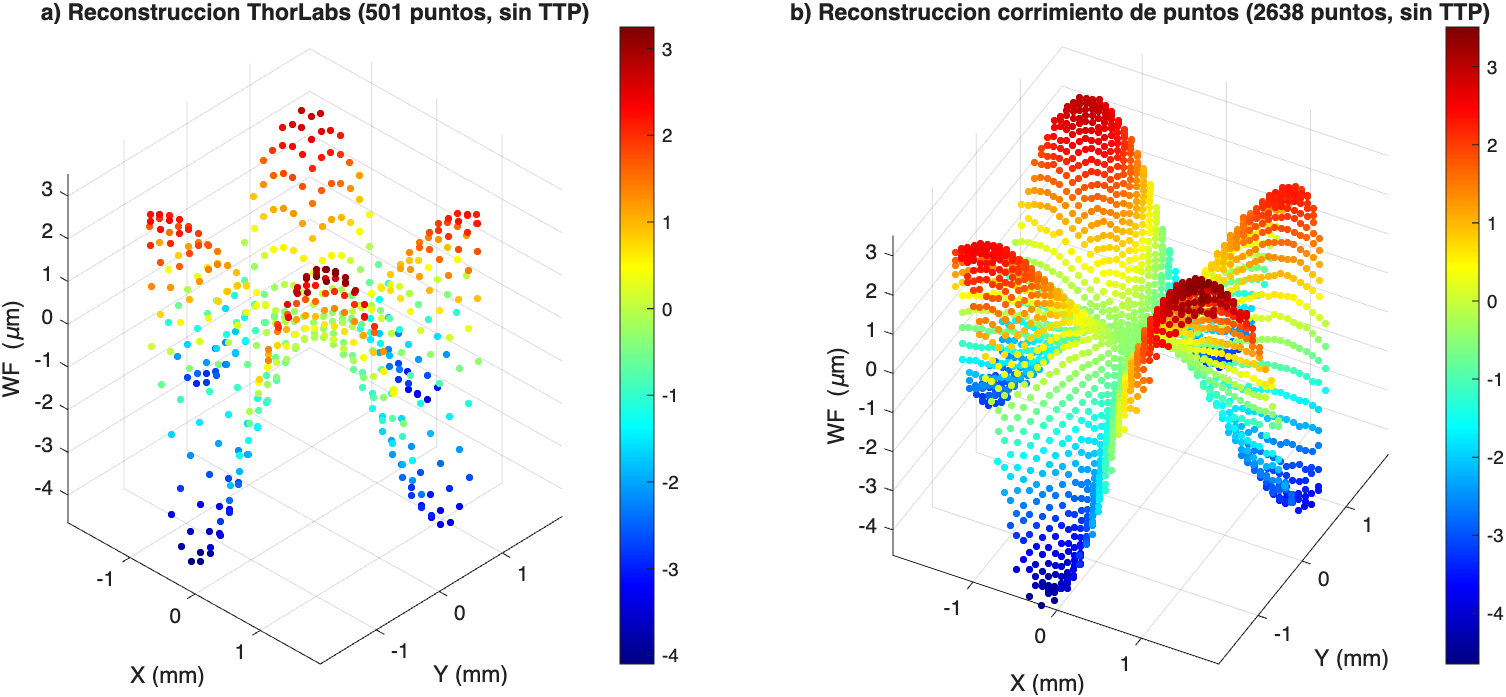
\includegraphics[width=\linewidth]{cap5-fig5_5_2-reconstruccion-sin-ttp-perspectiva.png}
  \caption{Reconstrucción del frente de onda en perspectiva tridimensional tras la
  remoción de tip, tilt y pistón. \textbf{a)} Reconstrucción de Thorlabs. \textbf{b)}
  Reconstrucción por el método de corrimiento de puntos. Eliminada la inclinación residual
  visible en la Fig.~\ref{fig:cap5-fig5-4-1}, ambos frentes de onda muestran la estructura
  asociada al modo tetrafoil $Z_{11}$ con magnitudes y formas comparables.}
  \label{fig:cap5-fig5-5-2}
\end{figure}

Tras la remoción de tip, tilt y pistón, la diferencia punto a punto entre ambas
reconstrucciones se reduce de los $1.16~\mu$m de la etapa previa al procesado
(Sección~\ref{sec:z11-reconstruccion-inicial}) a $0.145~\mu$m, evaluada por el mismo
procedimiento de emparejamiento por vecino más cercano. Esta reducción de casi un orden de
magnitud confirma cuantitativamente lo que la inspección visual sugiere: la mayor parte
del residuo directo correspondía al desajuste de modos bajos entre los dos métodos, no a
un error genuino del método de corrimiento de puntos. La atribución no es intuitiva sino
aritmética: el ajuste de plano tiene sólo tres grados de libertad (tip, tilt y pistón) y
no puede absorber estructura de orden superior, de modo que la caída de $1.16$ a
$0.145~\mu$m indica que cerca del 88~\% del residuo directo estaba en esos tres términos;
y esos términos no son información del frente de onda que se pierda, porque ninguno de los
dos métodos los mide de forma absoluta (Sección~\ref{sec:diferencia}). El residuo restante
de $0.145~\mu$m es la métrica de fidelidad sobre la que se realiza la validación
cuantitativa del método para esta primera evaluación. Como orden de magnitud, equivale a
$\lambda/4.4$ a $635$~nm; es mayor que la exactitud nominal del sensor ($\lambda/30$,
Tabla~\ref{tab:ap-wfs}), lo cual es esperable porque no mide el error del sensor sino la
diferencia entre dos algoritmos de reconstrucción distintos aplicados sobre dominios de
muestreo distintos.

\subsection{Comparación como superficie continua: incremento de resolución espacial}\label{sec:z11-trisurf}

Las visualizaciones por nube de puntos de las
Secciones~\ref{sec:z11-reconstruccion-inicial} y~\ref{sec:z11-reconstruccion-sin-ttp}
permiten comparar la magnitud y la forma global del frente de onda, pero la diferencia en
densidad de muestreo entre ambas reconstrucciones queda parcialmente oculta cuando los
puntos se solapan. Para hacer evidente esa diferencia representamos cada reconstrucción
como una superficie triangulada continua, obtenida por triangulación de Delaunay sobre los
puntos disponibles. La Fig.~\ref{fig:cap5-fig5-6-1} muestra esta representación en
perspectiva tridimensional para ambos frentes de onda residuales (sin tip, tilt ni
pistón). Vista a esta escala, las dos superficies presentan la misma forma global asociada
al modo tetrafoil $Z_{11}$ y una amplitud vertical comparable; la diferencia entre ellas,
$0.145~\mu$m RMS según la subsección anterior, es pequeña frente a esa amplitud.

\begin{figure}[htbp]
  \centering
  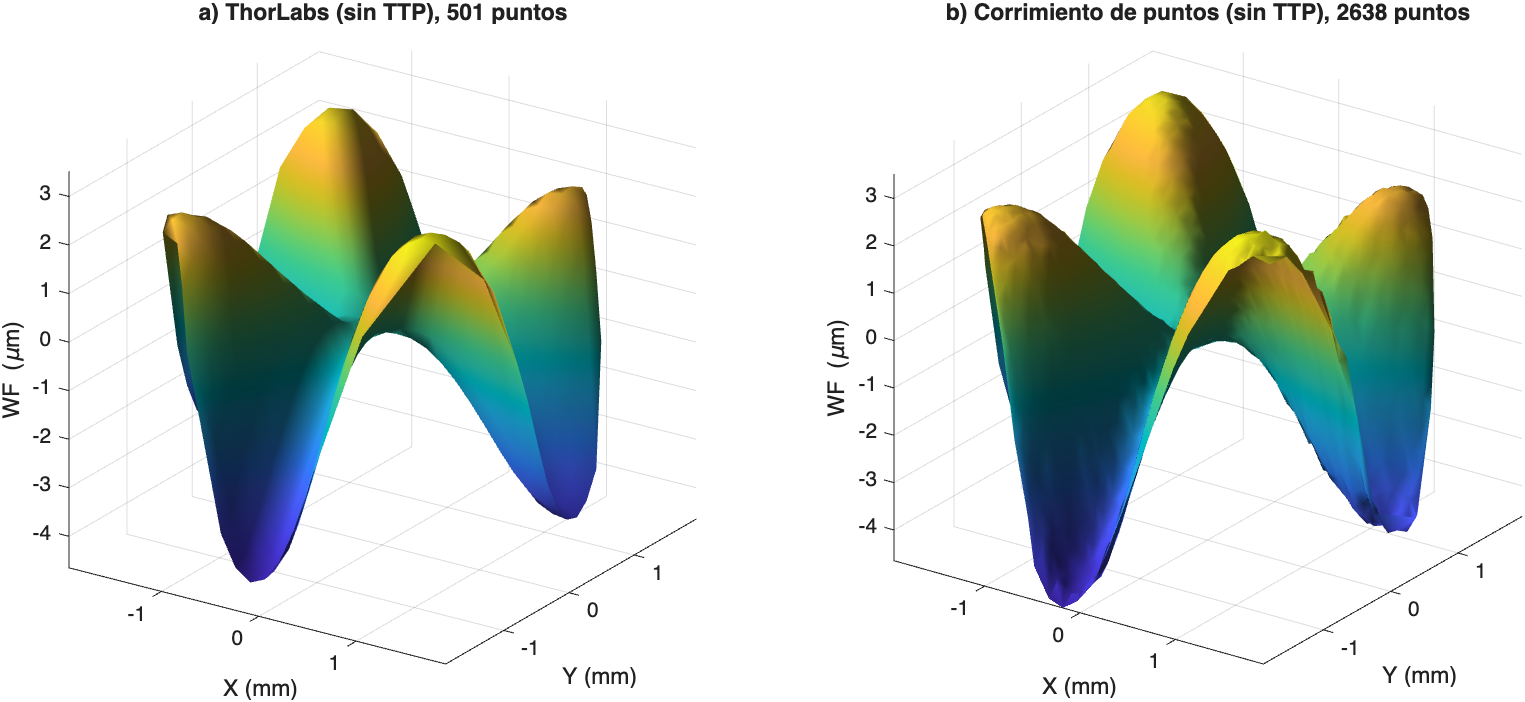
\includegraphics[width=\linewidth]{cap5-fig5_6_1-trisurf-perspectiva-lejos.png}
  \caption{Reconstrucción del frente de onda como superficie triangulada (Delaunay), con
  tip, tilt y pistón removidos. \textbf{a)} Reconstrucción de Thorlabs sobre la malla
  canónica de microlentes (501 puntos). \textbf{b)} Reconstrucción por el método de
  corrimiento de puntos sobre la lista densificada (2638 puntos). Ambas superficies
  presentan la misma forma global asociada al modo tetrafoil $Z_{11}$.}
  \label{fig:cap5-fig5-6-1}
\end{figure}

La diferencia entre ambas reconstrucciones, que a la escala completa de la pupila no se
aprecia visualmente, se vuelve evidente al examinar regiones acotadas de la superficie.
Las Figs.~\ref{fig:cap5-fig5-6-2} y~\ref{fig:cap5-fig5-6-3} muestran dos acercamientos a
regiones distintas del frente de onda reconstruido. En el panel izquierdo de cada figura,
la superficie del fabricante es una malla triangular cuyos vértices son los $501$ centros
de microlente del arreglo canónico: posiciones matemáticas definidas por el paso de
$0.150$~mm que declara el fabricante, no posiciones medidas. En el panel derecho, la
superficie obtenida por corrimiento de puntos tiene como vértices los $2638$ centroides de
la lista densificada, con una separación efectiva de $0.150/\sqrt{5} \approx 0.067$~mm, de
modo que cada triángulo tiene aproximadamente la quinta parte del área. Esta densificación
no es una interpolación de los datos canónicos: cada vértice adicional de la superficie
corresponde a un centroide medido en uno de los cinco spotgramas registrados, y la
pendiente local sobre la que se integró ese vértice proviene de una medida física
independiente. La triangulación únicamente conecta esos puntos para visualizar la
superficie, pero la información que define cada vértice es una observación experimental
directa, no una estimación interpolada a partir de los vecinos.

\begin{figure}[htbp]
  \centering
  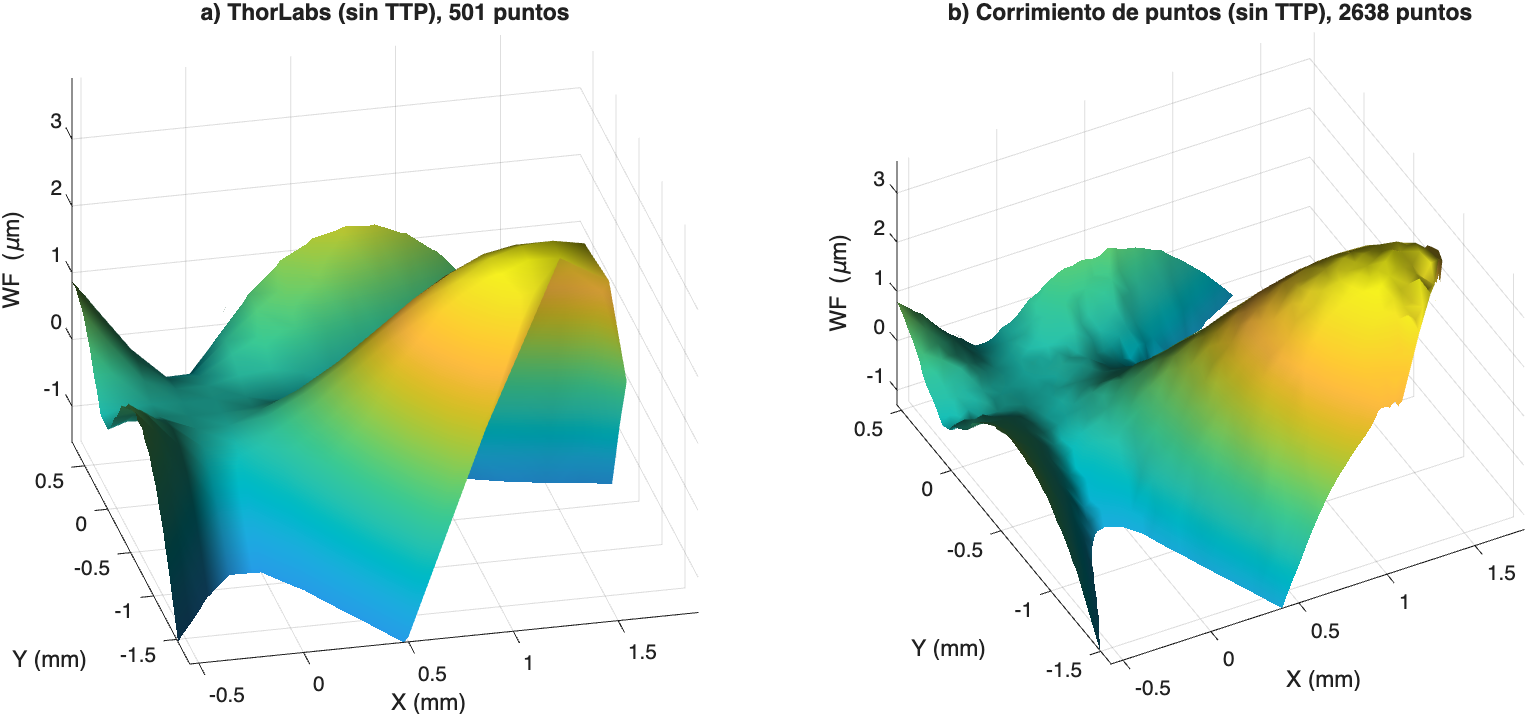
\includegraphics[width=\linewidth]{cap5-fig5_6_2-trisurf-closeup-1.png}
  \caption{Acercamiento a una primera región de la reconstrucción de la
  Fig.~\ref{fig:cap5-fig5-6-1}. \textbf{a)} Superficie triangulada sobre los puntos de
  Thorlabs. \textbf{b)} Superficie triangulada sobre los puntos del método de corrimiento
  de puntos. La densidad de muestreo es aproximadamente cinco veces mayor en \textbf{b)},
  conforme al factor $\varepsilon = m^2 + n^2 = 5$.}
  \label{fig:cap5-fig5-6-2}
\end{figure}

\begin{figure}[htbp]
  \centering
  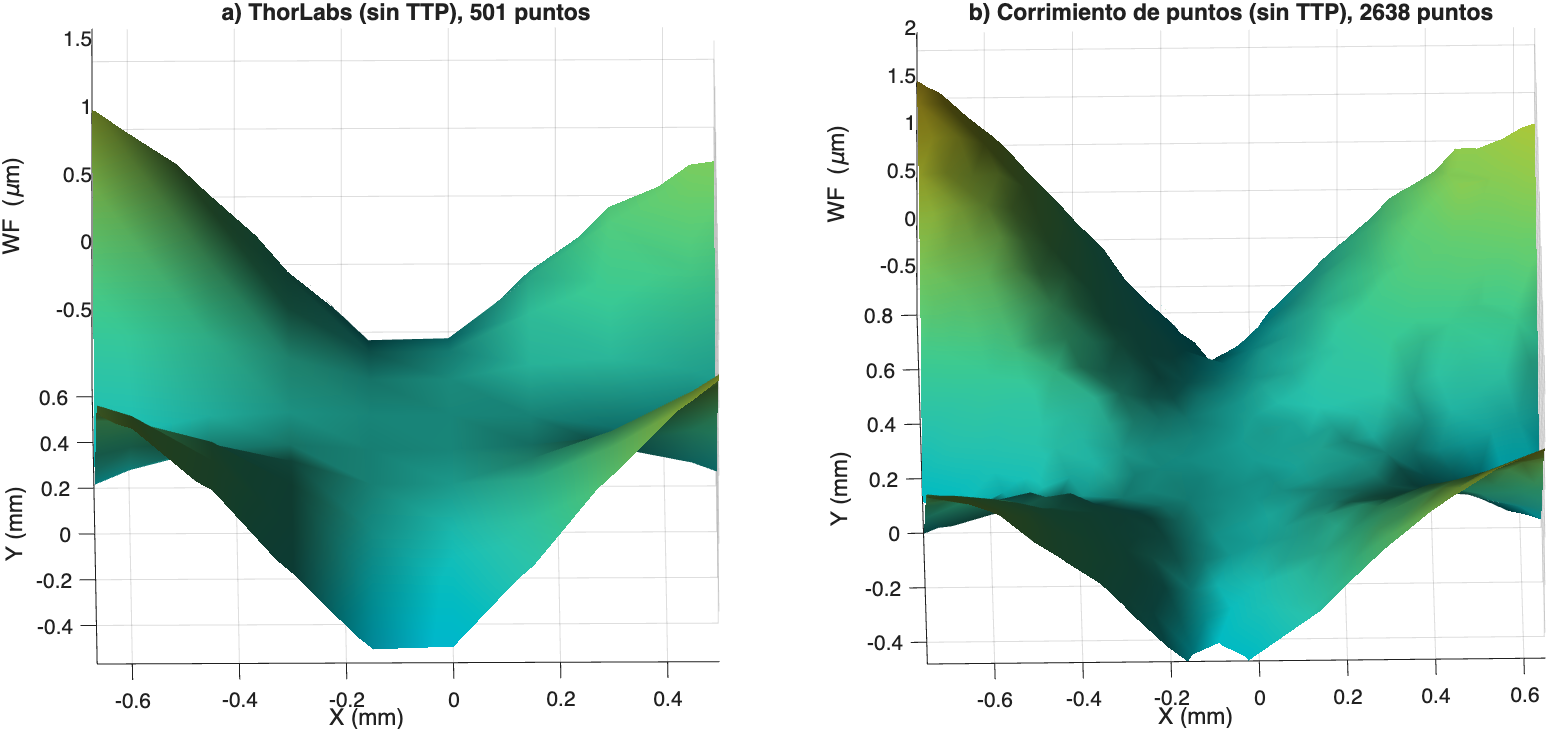
\includegraphics[width=\linewidth]{cap5-fig5_6_3-trisurf-closeup-2.png}
  \caption{Acercamiento a una segunda región de la reconstrucción de la
  Fig.~\ref{fig:cap5-fig5-6-1}. \textbf{a)} Thorlabs. \textbf{b)} Corrimiento de puntos.
  Cada vértice adicional de la superficie en \textbf{b)} corresponde a un centroide medido
  en uno de los cinco spotgramas adquiridos, no a una interpolación de los datos
  canónicos.}
  \label{fig:cap5-fig5-6-3}
\end{figure}

\subsection{Resumen cuantitativo de la primera evaluación}\label{sec:z11-tabla-resumen}

La Tabla~\ref{tab:cap5-resumen-eval1} concentra los parámetros geométricos de la región
evaluada, los planos (tip, tilt y pistón) restados a cada reconstrucción y las dos
métricas de fidelidad usadas en este trabajo: el RMS de la diferencia entre ambas
reconstrucciones antes y después de la remoción de tip, tilt y pistón. Solo se reportan
estas dos métricas porque, como se argumentó en la Sección~\ref{sec:rms}, en una
evaluación con aberración no nula el RMS de un único frente de onda describe la magnitud
de la aberración impuesta, no la fidelidad del método; la fidelidad sólo queda definida
cuando se compara contra una referencia. Esa referencia no es aquí un frente de onda
conocido de antemano, que no se tiene (Sección~\ref{sec:sistema-optico}), sino la
reconstrucción que el software del fabricante produce a partir de las mismas mediciones:
dos algoritmos distintos aplicados a los mismos centroides deben describir el mismo frente
de onda, y la métrica de fidelidad mide cuánto difieren después de remover los términos
que ninguno de los dos fija de forma absoluta (Sección~\ref{sec:comparacion}).

\begin{table}[htbp]
\centering
\caption{Resumen cuantitativo de la primera evaluación: dirección $(m,n)=(1,2)$,
aberración $Z_{11}$ (tetrafoil), amplitud relativa del software $-0.99$.}
\label{tab:cap5-resumen-eval1}
\small
\begin{tabularx}{\textwidth}{>{\raggedright\arraybackslash}Xl}
\hline
\textbf{Cantidad} & \textbf{Valor} \\
\hline
Puntos reconstruidos (lista densificada) & $2638$ \\
Puntos canónicos (referencia Thorlabs)   & $501$ \\
Caminos de integración depurados         & $1271$ \\
Radio de selección $R$                   & $1.95$~mm \\
Cota de vecindad                         & $0.0948$~mm \\
\hline
Plano restado, corrimiento de puntos $(a, b, c)$ & $(1.6\times 10^{-3},\ \approx 0,\ 5\times 10^{-4})$ \\
Plano restado, Thorlabs $(a, b, c)$              & $(5.06\times 10^{-4},\ 5.14\times 10^{-4},\ 2.58\times 10^{-4})$ \\
\hline
RMS diferencia directa                   & $1.16~\mu$m \\
RMS diferencia tras TTP independiente    & $0.145~\mu$m \\
\hline
\end{tabularx}
\end{table}

\section[Segunda evaluación: dirección (m,n)=(1,2), aberración Z13 negativa]{Segunda evaluación: dirección \mbox{$(m,n)=(1,2)$}, aberración $Z_{13}$ negativa}\label{sec:eval-z13-m1n2}

La segunda evaluación mantiene la dirección de barrido $(m,n)=(1,2)$ con factor de
densificación $\varepsilon = 5$ y los mismos cinco desplazamientos $\sigma_i \in
\{-0.1342,\allowbreak\,-0.0671,\allowbreak\,0,\allowbreak\,+0.0671,\allowbreak\,+0.1342\}$~mm;
lo que cambia respecto a la primera evaluación es la aberración impuesta por el espejo
deformable: el modo $Z_{13}$ (esférica primaria, Tabla~\ref{tab:modos-dm}) con amplitud
relativa del software en $-0.97$. Por compartir dirección y número de corrimientos con la
evaluación anterior, los pasos del procedimiento son idénticos y se reportan aquí de
manera condensada, presentando únicamente las figuras y métricas que dan cuenta del
resultado.

\begin{figure}[htbp]
  \centering
  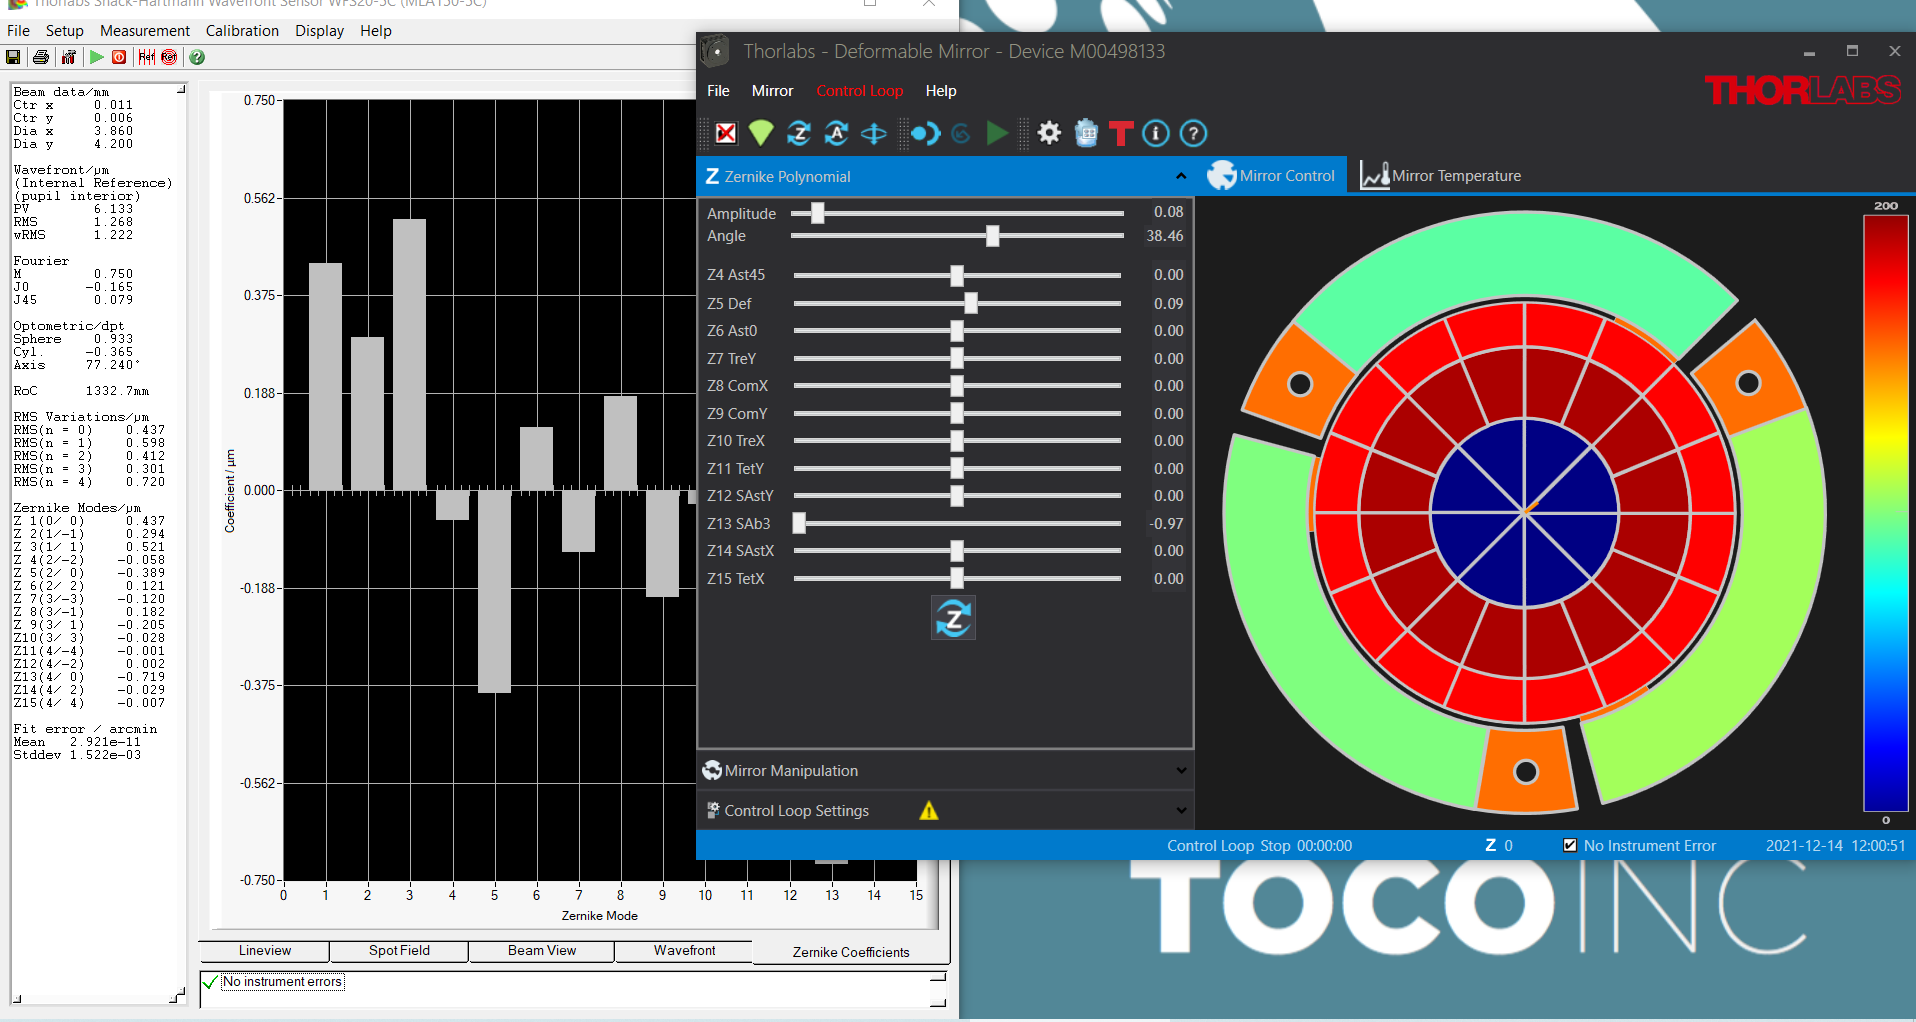
\includegraphics[width=0.95\linewidth]{cap5-eval2-fig1-setup-thorlabs.png}
  \caption{Estado inicial del experimento para la segunda evaluación, capturado desde la
  interfaz en vivo del software del fabricante (\textit{WFS Series Wavefront Analysis
  Software}, Thorlabs) en la posición central $\sigma=0$, con el espejo deformable
  configurado en el modo $Z_{13}$ (\textit{SAb3}, esférica primaria;
  Tabla~\ref{tab:modos-dm}) en su valor negativo. La captura muestra simultáneamente el
  shack-hartmanngrama, la reconstrucción del frente de onda y los coeficientes de Zernike
  reportados por el software. Esta figura se incluye como referencia del estado
  experimental; no se utiliza en el análisis cuantitativo.}
  \label{fig:cap5-eval2-fig1}
\end{figure}

De partida, la Fig.~\ref{fig:cap5-eval2-fig1} documenta el estado experimental, capturada
desde la interfaz en vivo del software del fabricante en la posición central $\sigma=0$.
La pestaña de control del espejo deformable muestra el modo $Z_{13}$ (\textit{SAb3},
esférica primaria) en su deslizador de amplitud en $-0.97$, configuración que se mantiene
fija durante la adquisición de los cinco spotgramas; los demás modos del espejo permanecen
en cero. La descomposición en coeficientes de Zernike reportada por el software se incluye
únicamente como referencia del estado experimental y no se utiliza en el análisis
cuantitativo.

Sobre los cinco spotgramas adquiridos se aplica el procedimiento descrito en el
Capítulo~\ref{cap:metodologia}: composición de los $\varepsilon$ corrimientos, recorte a
una región circular y reconstrucción del frente de onda mediante integración por la regla
del trapecio sobre los caminos depurados. Para esta evaluación el radio de selección se
fija en $R = 2.10$~mm (correspondiente a $14$ veces el paso del arreglo de microlentes),
elección que se discute más adelante a la luz de la región efectiva en la que el software
del fabricante entrega su reconstrucción. La Fig.~\ref{fig:cap5-eval2-fig2} muestra la
lista densificada de centroides con la frontera circular superpuesta y el frente de onda
reconstruido en vista cenital, todavía con tip, tilt y pistón residuales presentes.

\begin{figure}[htbp]
  \centering
  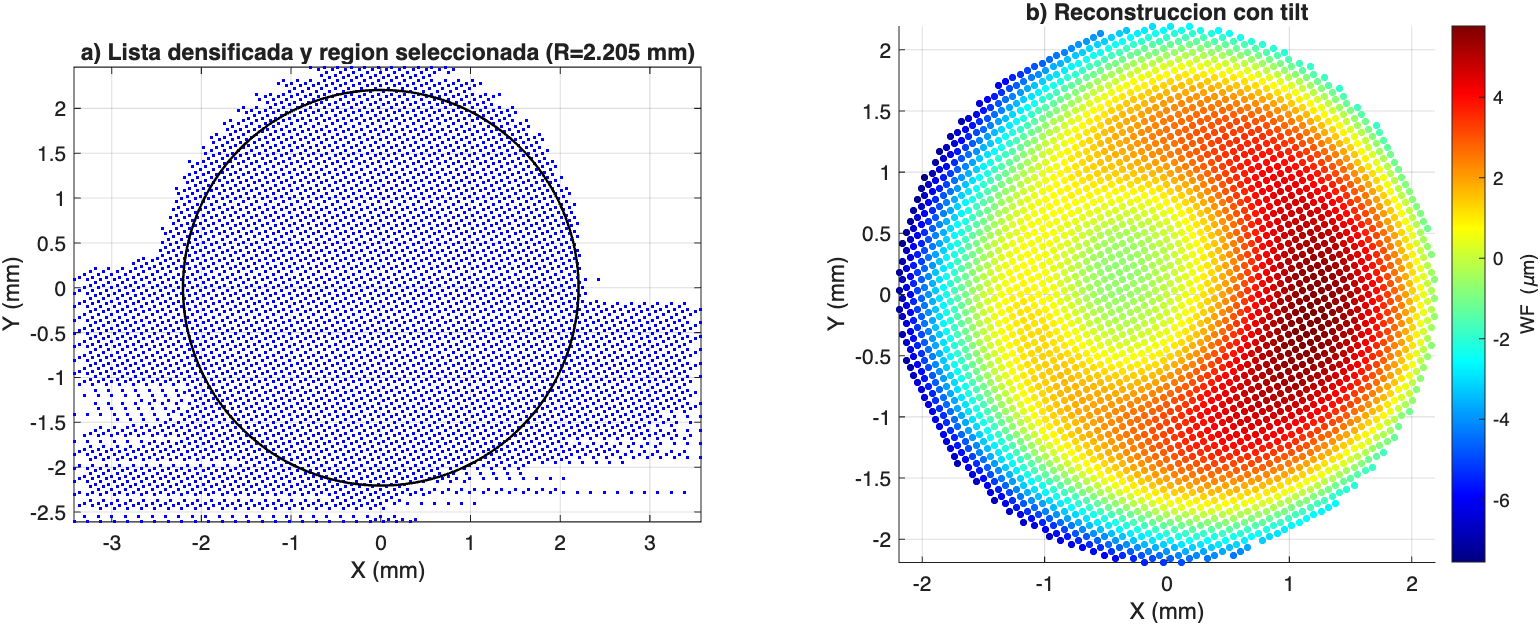
\includegraphics[width=\linewidth]{cap5-eval2-fig2-seleccion-recon-tilt.png}
  \caption{\textbf{a)} Lista densificada de centroides obtenida por composición de los
  cinco corrimientos, con la frontera circular de radio $R=2.10$~mm superpuesta como
  criterio de selección. \textbf{b)} Reconstrucción inicial del frente de onda en vista
  cenital, todavía con tip, tilt y pistón residuales; el color codifica la altura del
  frente de onda reconstruido en cada centro de microlente.}
  \label{fig:cap5-eval2-fig2}
\end{figure}

Tras la remoción de tip, tilt y pistón a cada frente de onda por mínimos cuadrados, las
dos reconstrucciones quedan en una escala vertical comparable. La
Fig.~\ref{fig:cap5-eval2-fig3} las presenta lado a lado en vista cenital, con el color
codificando la altura: en ambos paneles se distingue la estructura del modo esférico
$Z_{13}$, con un borde anular elevado y una depresión central casi simétrica de revolución
sobre la pupila. La diferencia en densidad espacial entre los $503$ puntos canónicos del
fabricante y los $3082$ puntos de la lista densificada se manifiesta.

\begin{figure}[htbp]
  \centering
  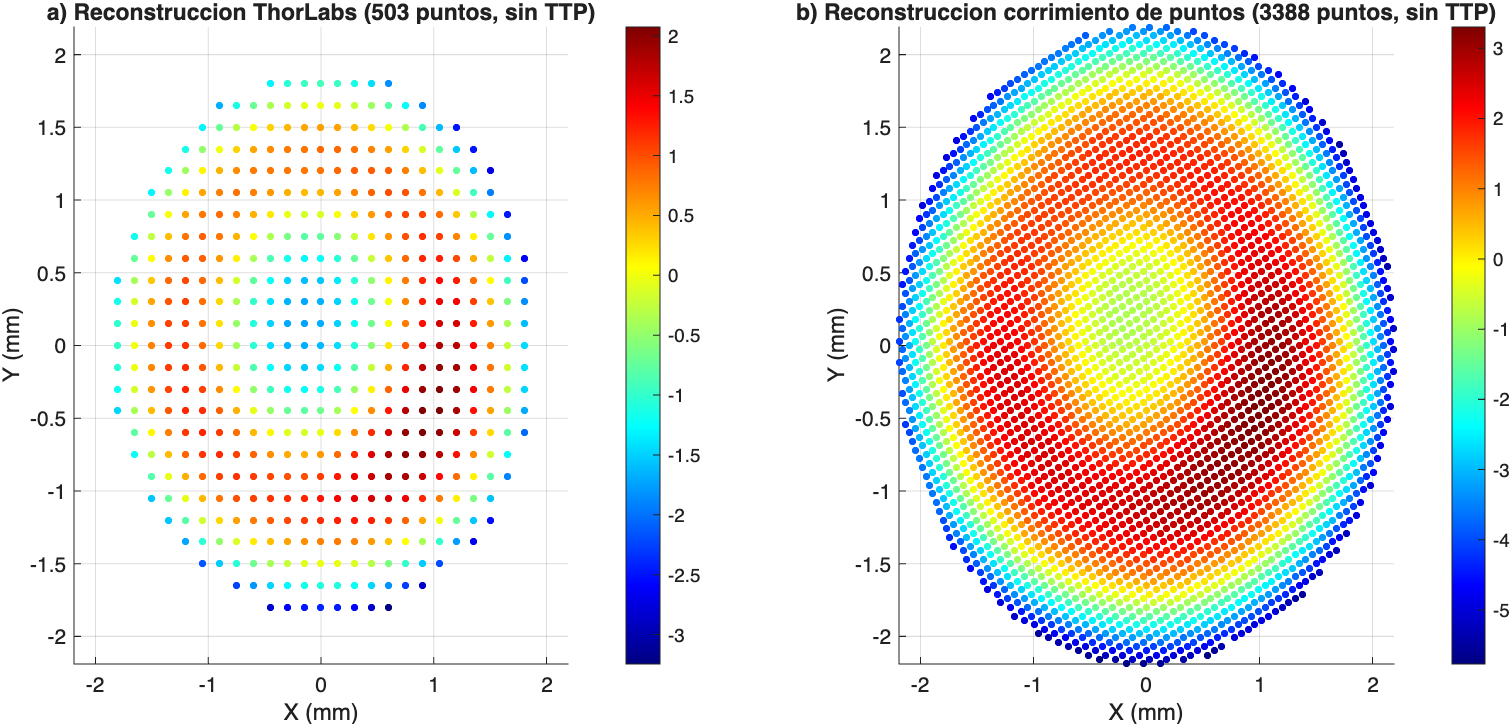
\includegraphics[width=\linewidth]{cap5-eval2-fig3-colorbar.png}
  \caption{Reconstrucción del frente de onda en vista cenital tras la remoción de tip,
  tilt y pistón. \textbf{a)} Reconstrucción de Thorlabs sobre la malla canónica de
  microlentes ($503$ puntos). \textbf{b)} Reconstrucción por el método de corrimiento de
  puntos sobre la lista densificada ($3082$ puntos). El color codifica la altura del
  frente de onda residual; ambos paneles comparten escala de color para comparación visual
  directa.}
  \label{fig:cap5-eval2-fig3}
\end{figure}

Una particularidad de esta evaluación, no observada con la misma claridad en la primera,
es que la región sobre la que el software del fabricante entrega su reconstrucción es
notablemente menor que la región sobre la que registra centroides válidos. La
Fig.~\ref{fig:cap5-eval2-fig4} ilustra esta diferencia: el panel \textbf{a)} muestra los
centroides medidos en la toma central $\sigma=0$ tal como los entrega el sensor (los
puntos cuya posición fue extraída satisfactoriamente), mientras que el panel \textbf{b)}
muestra únicamente los puntos del mallado de salida que el software del fabricante
reconstruye y reporta en su archivo de mesh. La diferencia entre ambos conjuntos no es
introducida por nuestro procesamiento: el sensor recoge centroides en una región más
amplia que la que el algoritmo modal del fabricante decide finalmente reconstruir. Esto
significa que, aunque el método de corrimiento de puntos puede reconstruir el frente de
onda en un área que se extiende hasta la frontera circular de selección, la comparación
cuantitativa contra Thorlabs queda restringida al área donde el fabricante reporta datos.
Para que el RMS de la diferencia se calcule sobre la misma región en ambos lados, los
puntos de Thorlabs se filtran por el radio $R$ antes del emparejamiento por vecino más
cercano, asegurando que sólo se comparen puntos dentro del círculo común; los puntos
extras que nuestra reconstrucción produce en la franja exterior no contribuyen a la
métrica reportada.

\begin{figure}[htbp]
  \centering
  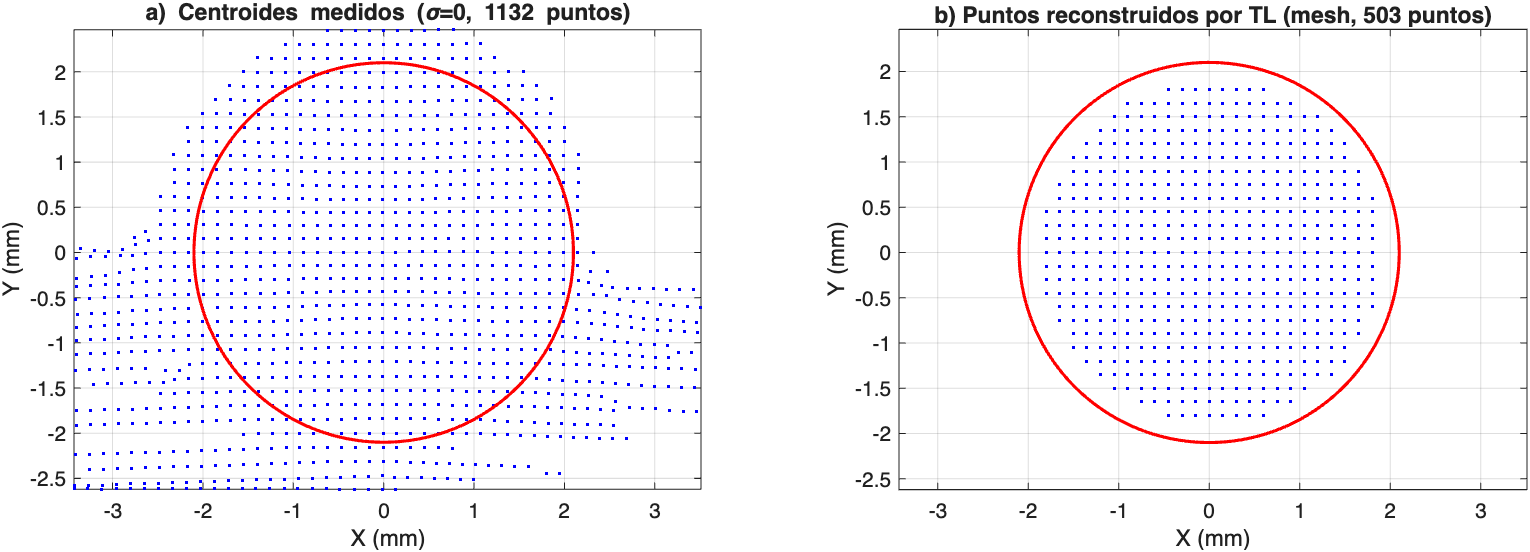
\includegraphics[width=\linewidth]{cap5-eval2-fig4-centroides-vs-mesh-tl.png}
  \caption{Comparación entre los centroides medidos por el sensor y los puntos que el
  software del fabricante reconstruye. \textbf{a)} Centroides extraídos de la toma central
  $\sigma=0$ tal como los entrega el sensor, con la frontera circular de radio $R$
  superpuesta. \textbf{b)} Puntos del mallado de salida que Thorlabs entrega en su archivo
  de reconstrucción, con la misma frontera. El subconjunto que el software reconstruye es
  notablemente más pequeño que el conjunto de centroides medidos; esta diferencia depende
  del algoritmo del fabricante y delimita la región sobre la que se realiza la comparación
  cuantitativa.}
  \label{fig:cap5-eval2-fig4}
\end{figure}

La Fig.~\ref{fig:cap5-eval2-fig5} presenta las mismas dos reconstrucciones de la
Fig.~\ref{fig:cap5-eval2-fig3} en perspectiva tridimensional, donde el eje $z$ explícito
en micrómetros permite apreciar la magnitud y la forma de la aberración esférica impuesta.
Ambas superficies comparten el mismo patrón global y escalas verticales del mismo orden,
lo que es coherente con la diferencia RMS reportada en la tabla resumen al final de esta
sección.

\begin{figure}[htbp]
  \centering
  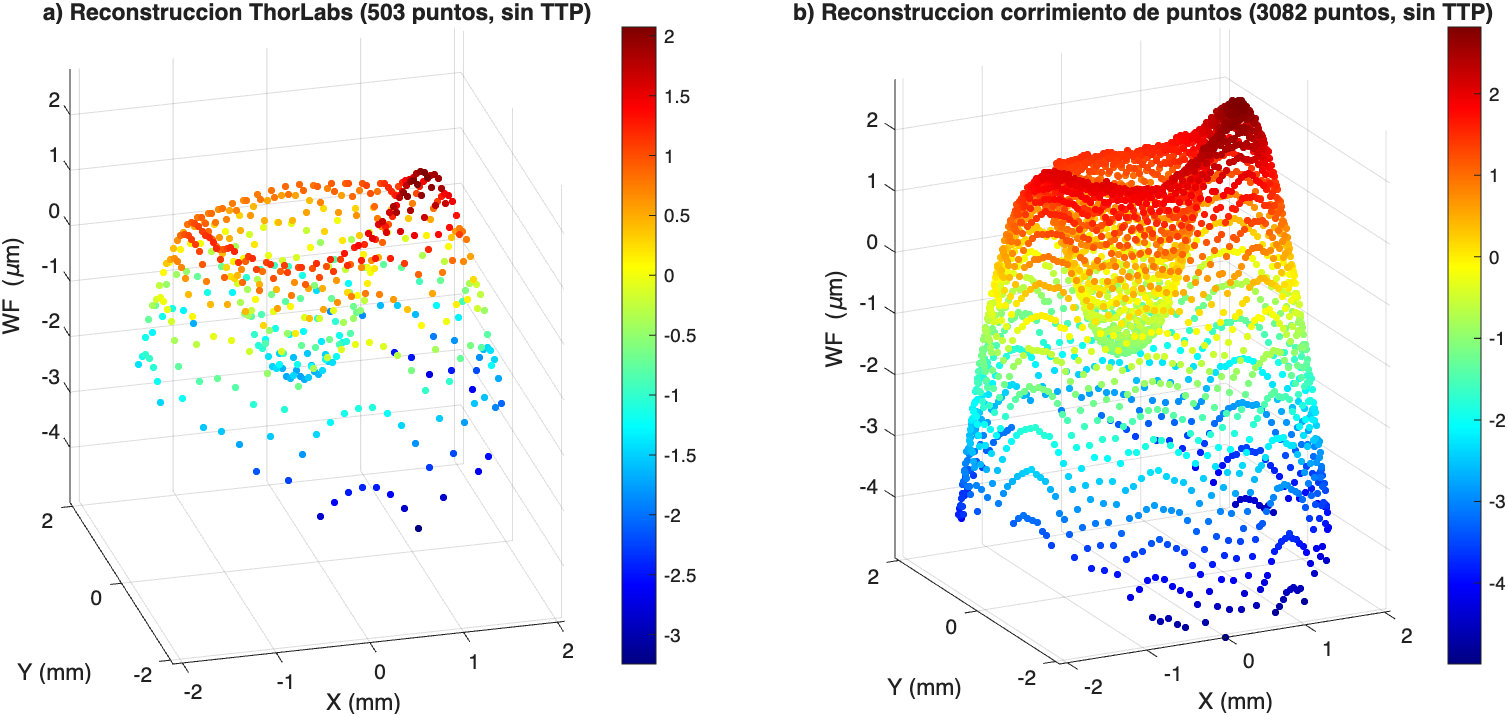
\includegraphics[width=\linewidth]{cap5-eval2-fig5-perspective-sin-ttp.png}
  \caption{Reconstrucción del frente de onda en perspectiva tridimensional tras la
  remoción de tip, tilt y pistón. \textbf{a)} Reconstrucción de Thorlabs. \textbf{b)}
  Reconstrucción por el método de corrimiento de puntos. Ambas superficies muestran el
  modo esférico $Z_{13}$ con magnitudes y formas comparables; la diferencia visible en
  densidad de muestreo entre paneles refleja el factor $\varepsilon=5$.}
  \label{fig:cap5-eval2-fig5}
\end{figure}

Para hacer evidente el incremento de resolución espacial representamos ambos frentes de
onda como superficies trianguladas (Delaunay) sin colormap por altura. La
Fig.~\ref{fig:cap5-eval2-fig6} muestra la vista global, donde las dos superficies
comparten la misma forma asociada al modo esférico.

\begin{figure}[htbp]
  \centering
  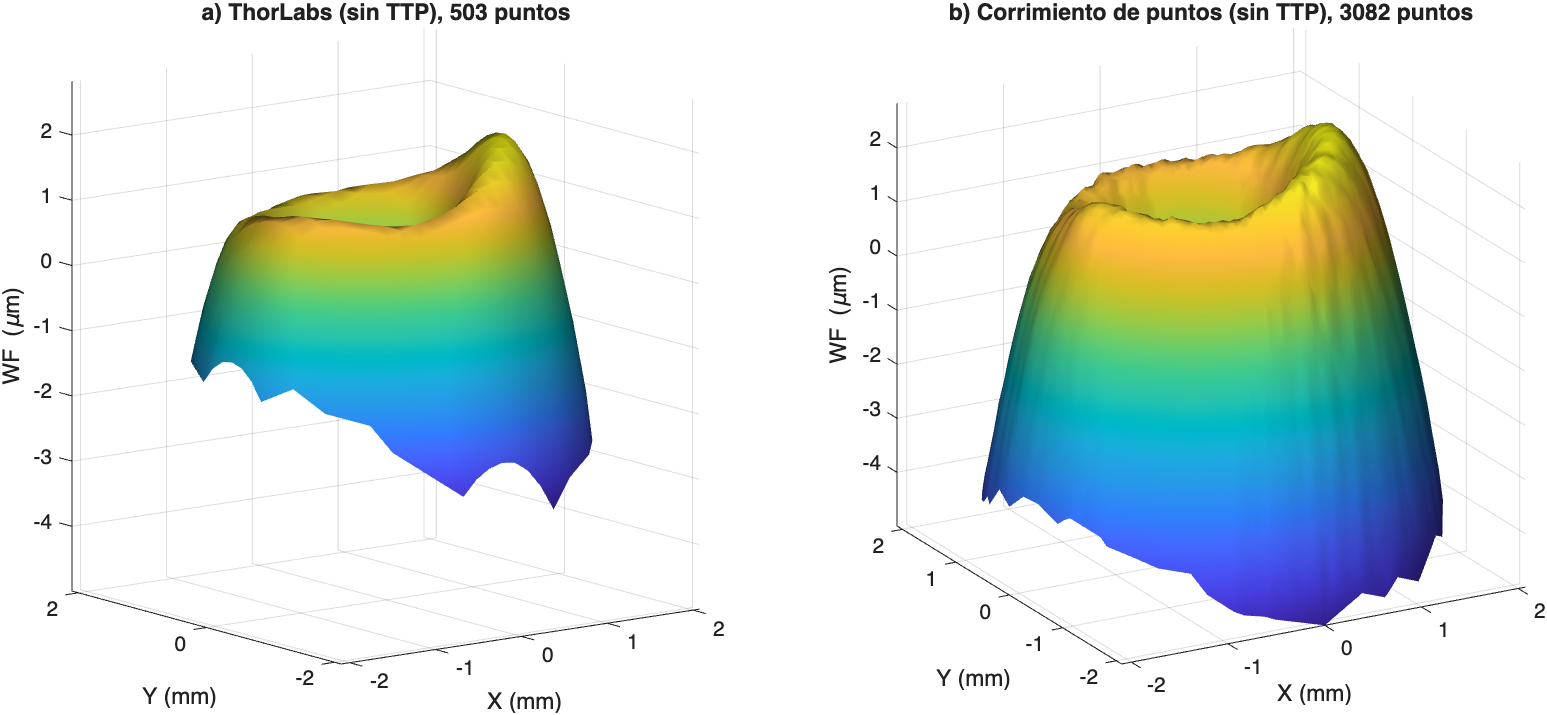
\includegraphics[width=\linewidth]{cap5-eval2-fig6-trisurf-sin-ttp.png}
  \caption{Reconstrucción del frente de onda como superficie triangulada (Delaunay), con
  tip, tilt y pistón removidos. \textbf{a)} Reconstrucción de Thorlabs. \textbf{b)}
  Reconstrucción por el método de corrimiento de puntos. Ambas superficies presentan la
  misma forma global asociada al modo esférico $Z_{13}$.}
  \label{fig:cap5-eval2-fig6}
\end{figure}

A escala completa de la pupila las dos superficies se ven prácticamente equivalentes; la
diferencia entre ambas se vuelve evidente al examinar regiones acotadas. La
Fig.~\ref{fig:cap5-eval2-fig7} muestra un acercamiento donde la diferencia en densidad de
la triangulación se hace inmediata, con caras de aproximadamente la quinta parte del área
en el panel del método de corrimiento de puntos. Como ya fue mencionado en la primera
evaluación, esta densificación no es interpolación: cada vértice adicional corresponde a
un centroide medido en uno de los cinco spotgramas adquiridos.

\begin{figure}[htbp]
  \centering
  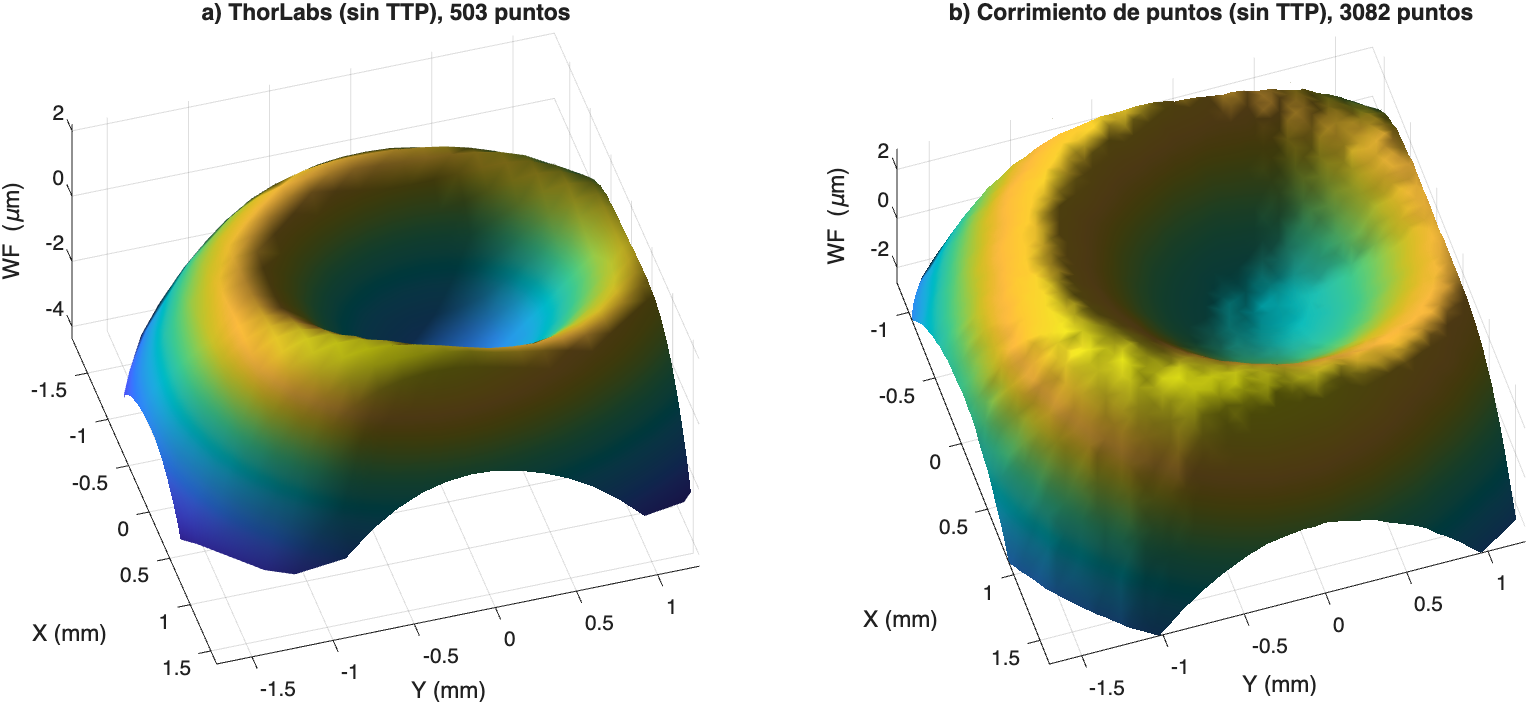
\includegraphics[width=\linewidth]{cap5-eval2-fig7-trisurf-acercamiento.png}
  \caption{Acercamiento a una región de la reconstrucción de la
  Fig.~\ref{fig:cap5-eval2-fig6}. \textbf{a)} Thorlabs. \textbf{b)} Corrimiento de puntos.
  La densidad de triangulación es aproximadamente cinco veces mayor en \textbf{b)},
  conforme al factor $\varepsilon=5$; cada vértice adicional corresponde a un centroide
  medido en uno de los cinco spotgramas, no a una interpolación.}
  \label{fig:cap5-eval2-fig7}
\end{figure}

\subsection{Análisis posterior: pistón residual entre superficies por muestreo asimétrico}\label{sec:eval2-segundo-tratamiento}

Al calcular el RMS de la diferencia tras la remoción de tip, tilt y pistón con el
procedimiento estándar (un ajuste de plano independiente para cada frente de onda) se
obtiene un valor de $0.67~\mu$m. Este valor es sensiblemente mayor que el residuo de la
primera evaluación ($0.145~\mu$m), y es más de lo que se puede atribuir únicamente al
cambio de aberración entre $Z_{11}$ y $Z_{13}$, así que antes de aceptar el resultado como
definitivo revisamos los datos. Revisando valor a valor en distintas regiones de la
pupila, se observa que la diferencia entre nuestro frente de onda y el del fabricante es
aproximadamente constante: en el centro $(0,0)$ es de $+0.54~\mu$m y en la cresta
$(0.75,-0.75)$ es de $+0.68~\mu$m. Las dos superficies tienen formas comparables pero
quedan desplazadas verticalmente entre sí en una cantidad casi uniforme; pese al ajuste de
plano por mínimos cuadrados aplicado a cada frente de onda, persiste un \emph{pistón
residual} entre las dos reconstrucciones.

Para visualizar este sesgo y diseñar una corrección, se mapea la diferencia $\Delta = W -
W_{\text{TL}}$ punto a punto sobre la pupila, primero como aparece directamente y después
tras cada paso de procesado. La Fig.~\ref{fig:cap5-eval2-diferencias-tres-etapas}
concentra esa información en tres paneles.

\begin{figure}[htbp]
  \centering
  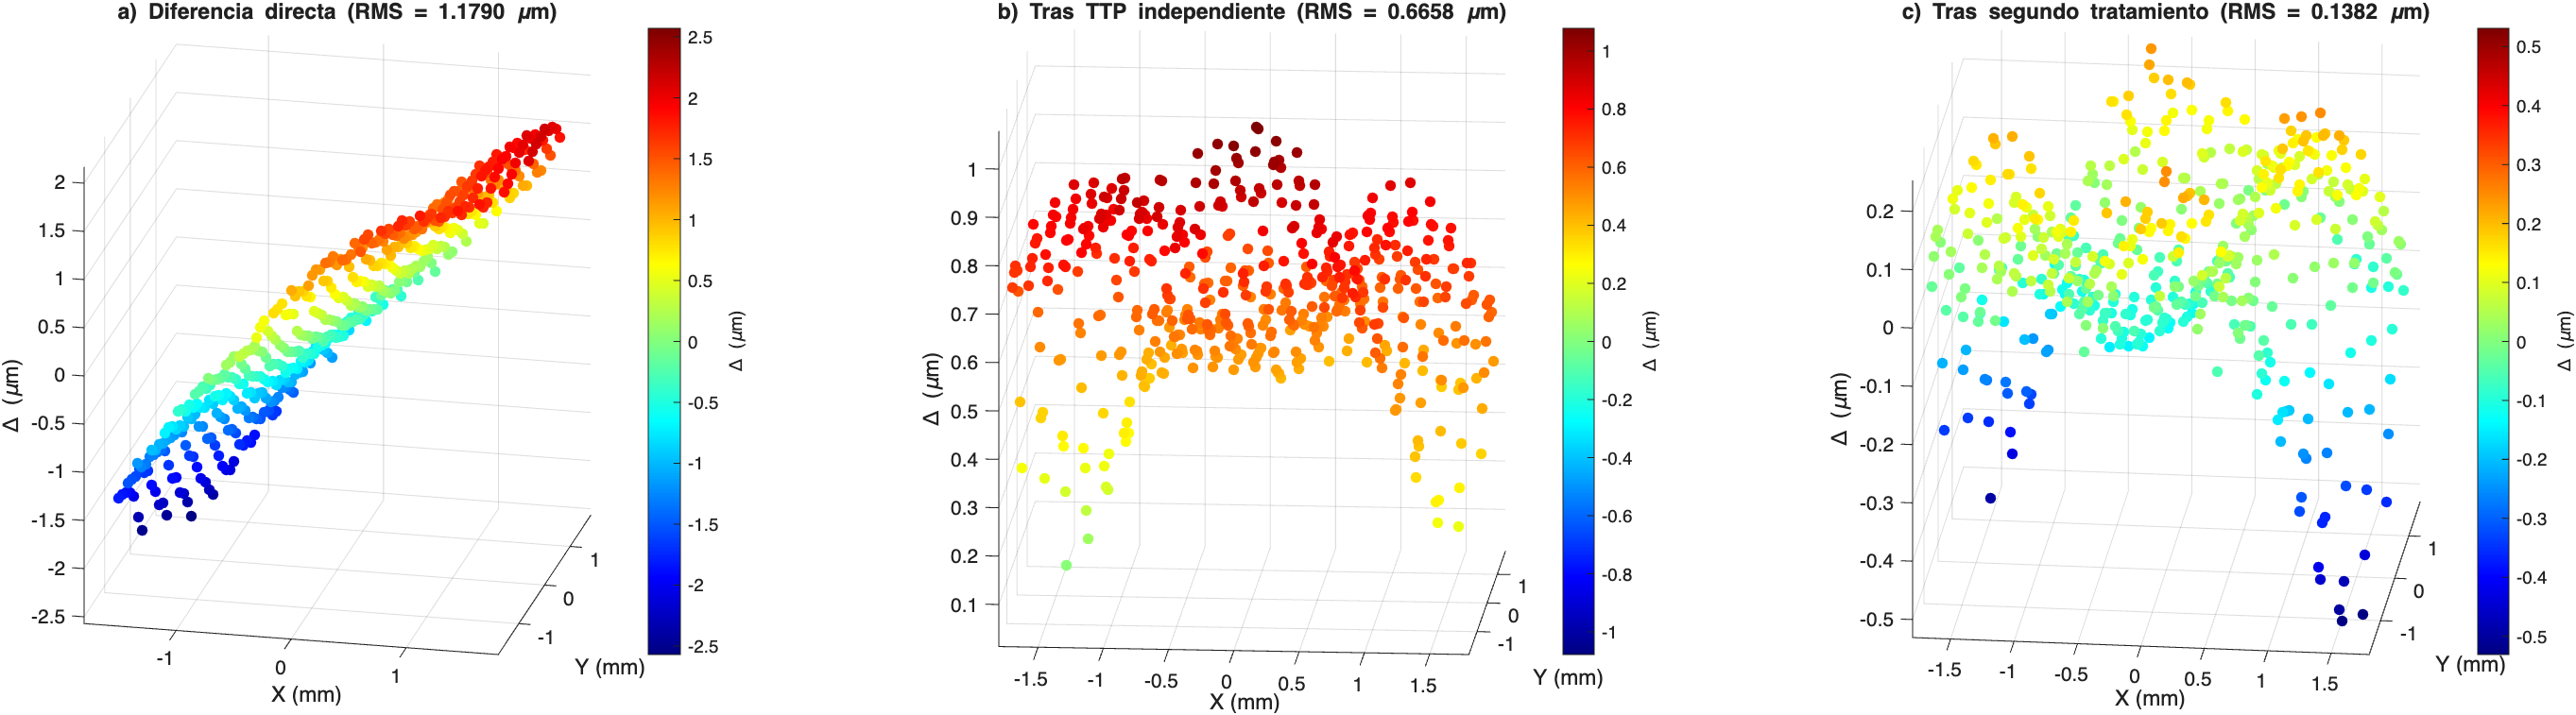
\includegraphics[width=\linewidth]{cap5-eval2-diferencias-tres-etapas.png}
  \caption{Diferencia $\Delta = W - W_{\text{TL}}$ punto a punto sobre la pupila, en tres
  etapas sucesivas de procesado, cada una con su escala de color simétrica alrededor de
  cero. \textbf{a)} Diferencia directa, antes de cualquier corrección, dominada por la
  pendiente común del montaje (RMS = $1.18~\mu$m). \textbf{b)} Tras ajuste TTP
  independiente a cada frente de onda: tip y tilt removidos, pero persiste un pistón
  relativo de $\sim 0.6~\mu$m (RMS = $0.67~\mu$m). \textbf{c)} Tras el segundo
  tratamiento: plano ajustado a la diferencia y restado; el pistón residual desaparece
  (RMS = $0.14~\mu$m).}
  \label{fig:cap5-eval2-diferencias-tres-etapas}
\end{figure}

El panel \textbf{(a)} corresponde a la diferencia directa y muestra una pendiente clara
que recorre la pupila de un extremo al otro: tip y tilt residuales del montaje son los
modos dominantes en este punto del análisis, con un RMS de $1.18~\mu$m. El panel
\textbf{(b)} es el resultado del procedimiento estándar de remoción de TTP: la pendiente
desaparece, pero queda un offset prácticamente uniforme cuyo valor coincide con la
diferencia constante observada en la inspección punto a punto. Es exactamente este pistón
residual el que el ajuste TTP independiente no es capaz de cancelar, y la razón es
directa: los planos de mejor ajuste se calculan sobre dominios de muestreo distintos
($3082$ puntos densificados frente a $503$ puntos canónicos de Thorlabs) y la diferencia
de densidad pondera de forma desigual las regiones donde cada método tiene más muestras,
dejando los planos resultantes ligeramente inclinados de forma distinta y, por tanto,
dejando un offset relativo cuando se restan a sus respectivos frentes de onda. El panel
\textbf{(c)} muestra el efecto del segundo tratamiento: en lugar de ajustar dos planos
individuales, se ajusta un único plano por mínimos cuadrados a la propia diferencia
$\Delta$ y se le resta. El pistón relativo desaparece y el RMS cae a $0.14~\mu$m, una
reducción de aproximadamente cuatro veces respecto al estado anterior.

Una vez identificada y corregida la fuente del sesgo, repetimos la comparación
tridimensional entre las dos reconstrucciones para verificar visualmente que la corrección
es consistente con lo observado en los datos numéricos. La
Fig.~\ref{fig:cap5-eval2-post-2do-desplazamiento} presenta esa comparación final, en tres
vistas, sobre la misma región evaluada por Thorlabs.

\begin{figure}[htbp]
  \centering
  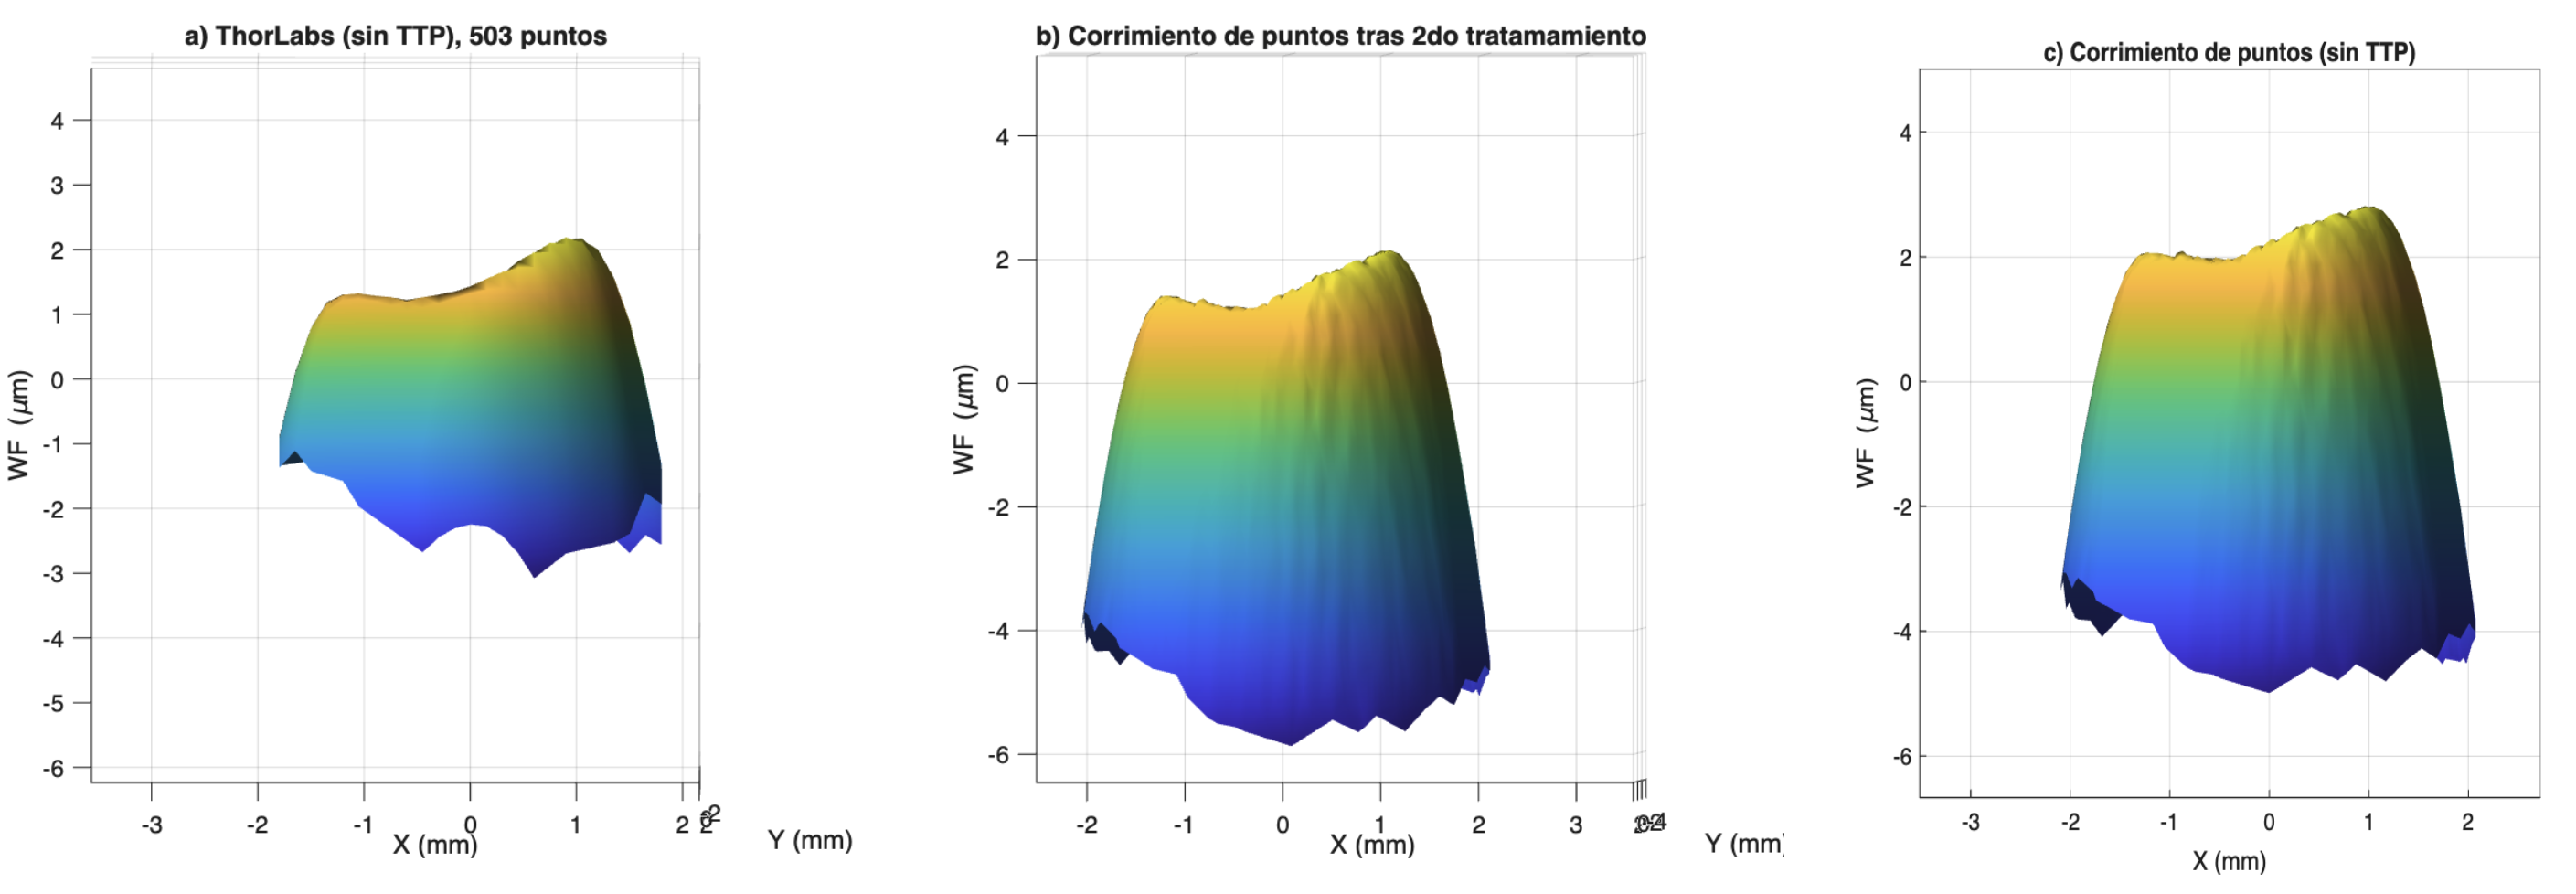
\includegraphics[width=\linewidth]{cap5-eval2-trisurf-post-2do-desplazamiento.png}
  \caption{Reconstrucción del frente de onda tras el segundo tratamiento, en tres vistas
  (a, b, c). La forma del modo esférico $Z_{13}$ aparece preservada en ambas
  reconstrucciones, ahora alineadas verticalmente; el método de corrimiento de puntos
  cubre la misma región evaluada por Thorlabs con un número considerablemente mayor de
  puntos.}
  \label{fig:cap5-eval2-post-2do-desplazamiento}
\end{figure}

Las dos reconstrucciones presentan ahora la misma forma del modo esférico $Z_{13}$ y a la
misma altura, sin el desplazamiento relativo que las separaba antes. Hay que precisar que
esta comparación se hace explícitamente sobre el área que Thorlabs reconstruye, no sobre
toda la región que el método de corrimiento de puntos cubre; en esa misma área, nuestra
reconstrucción contiene un número considerablemente mayor de puntos (lista densificada
frente al mallado canónico del fabricante), de modo que entrega una versión espacialmente
más resuelta del mismo frente de onda sobre el mismo dominio comparable. La concordancia
visual y el descenso del RMS de $0.67$ a $0.14~\mu$m sostienen, en conjunto, que el
segundo tratamiento era necesario para que la métrica reportada describa el error real
entre las dos reconstrucciones y no el sesgo de pistón introducido por la diferencia de
muestreos. La cifra de $0.14~\mu$m es la métrica de fidelidad representativa de esta
evaluación.

\subsection{Resumen cuantitativo de la segunda evaluación}\label{sec:z13-tabla-resumen}

La Tabla~\ref{tab:cap5-resumen-eval2} recoge los valores resultantes del análisis para
referencia.

\begin{table}[htbp]
\centering
\caption{Resumen cuantitativo de la segunda evaluación: dirección $(m,n)=(1,2)$,
aberración $Z_{13}$ (esférica primaria), amplitud relativa del software $-0.97$.}
\label{tab:cap5-resumen-eval2}
\small
\begin{tabularx}{\textwidth}{>{\raggedright\arraybackslash}Xl}
\hline
\textbf{Cantidad} & \textbf{Valor} \\
\hline
Puntos reconstruidos (lista densificada) & $3082$ \\
Puntos canónicos (referencia Thorlabs)   & $503$ \\
Caminos de integración depurados         & $1484$ \\
Radio de selección $R$                   & $2.10$~mm \\
Cota de vecindad                         & $0.0948$~mm \\
\hline
Plano restado, corrimiento de puntos $(a, b, c)$ & $(1.71\times 10^{-3},\ 1.97\times 10^{-5},\ 1.07\times 10^{-3})$ \\
Plano restado, Thorlabs $(a, b, c)$              & $(5.57\times 10^{-4},\ 3.18\times 10^{-4},\ 1.61\times 10^{-3})$ \\
\hline
RMS diferencia directa                          & $1.18~\mu$m \\
RMS diferencia tras TTP independiente       & $0.67~\mu$m \\
RMS diferencia tras segundo tratamiento     & $0.14~\mu$m \\
\hline
\end{tabularx}
\end{table}

\section[Tercera evaluación: dirección (m,n)=(1,3), aberración Z13 negativa]{Tercera evaluación: dirección \mbox{$(m,n)=(1,3)$}, aberración $Z_{13}$ negativa}\label{sec:eval-z13-m1n3}

La tercera evaluación cambia la dirección de barrido a $(m,n)=(1,3)$, lo que implica un
factor de densificación $\varepsilon = m^2 + n^2 = 10$ y un ángulo de rotación del sensor
$\theta_r = \arctan(1/3) \approx 18.43^\circ$. La configuración del espejo deformable se
mantiene nominalmente igual a la de la segunda evaluación: el mismo modo $Z_{13}$
\textit{SAb3} (esférica primaria según la Tabla~\ref{tab:modos-dm}) en amplitud negativa,
con el deslizador registrado en $-0.92$ para esta adquisición (frente a $-0.97$ en la
segunda evaluación); el frente de onda incidente sobre el arreglo de microlentes es, por
tanto, de la misma forma y magnitud comparable, aunque no idéntica. Esta diferencia no
compromete la evaluación: la amplitud del deslizador es una magnitud relativa sin
calibración absoluta: es un valor del software de control, no una medida del frente de
onda (Secciones~\ref{sec:convencion-zernike} y~\ref{sec:sistema-optico}), de modo que el
frente de onda efectivamente producido queda caracterizado por la propia medición del
sensor, y en cada evaluación la comparación se realiza contra la reconstrucción del
fabricante calculada sobre esas mismas mediciones (Sección~\ref{sec:comparacion}). Las
modificaciones del montaje son consecuencia exclusivamente del cambio en la dirección de
barrido: la combinación de la platina AP180 y el goniómetro se reajusta para alcanzar el
ángulo $\theta_r = 18.43^\circ$ a partir de la posición invertida de referencia
(Sección~\ref{sec:control-desplazamiento-altura}); la altura efectiva del sensor cambia
con la rotación y se compensa con la mesa de altura variable; el paso del servomotor se
reprograma a $\sigma_{\text{step}} = P_L/\sqrt{\varepsilon} = 0.0474$~mm para producir los
$\varepsilon=10$ corrimientos requeridos por el método. Pese a la precisión nominal del
control mecánico, el cambio combinado de ángulo y altura puede introducir variaciones
residuales en la alineación que hay que tener presentes al interpretar las métricas de
fidelidad.

A diferencia de las dos evaluaciones anteriores, los $\varepsilon=10$ corrimientos no se
distribuyen simétricamente alrededor del origen geométrico: en este caso el barrido se
realizó cubriendo las posiciones $\sigma_i$ con índices enteros desde $-4$ hasta $+5$, lo
que corresponde a desplazamientos en el rango $[-0.1897,\,+0.2371]$~mm en pasos de
$0.0474$~mm. Esta asimetría es propia del esquema empleado y no afecta la validez del
método: la composición de los diez patrones produce, igualmente, una lista densificada con
$\varepsilon$ veces más muestras que el arreglo canónico de microlentes.

El estado experimental de partida se documenta en la Fig.~\ref{fig:cap5-eval3-fig1},
capturada desde la interfaz en vivo del software del fabricante en la posición central
$\sigma=0$. En ella se aprecia tanto la configuración del espejo deformable, nominalmente
igual a la de la segunda evaluación (modo $Z_{13}$ \textit{SAb3}, amplitud $-0.92$), como
el paso programado del servomotor correspondiente a la nueva dirección $(m,n)=(1,3)$.

Sobre los diez spotgramas adquiridos se aplica el procedimiento ya descrito: composición
de los $\varepsilon$ corrimientos para producir la lista densificada, recorte a una región
circular y reconstrucción del frente de onda por integración numérica sobre los caminos
depurados. Para esta evaluación el radio de selección se fija en $R = 2.10$~mm, el mismo
que en la segunda evaluación, lo que permite cubrir aproximadamente la región sobre la que
el software del fabricante reporta su reconstrucción. La Fig.~\ref{fig:cap5-eval3-fig2}
muestra la lista densificada con la frontera circular superpuesta y el frente de onda
reconstruido en vista cenital, todavía con tip, tilt y pistón residuales. La densidad
espacial es notablemente mayor que en las dos evaluaciones previas, consistente con el
factor $\varepsilon=10$.

\begin{figure}[htbp]
  \centering
  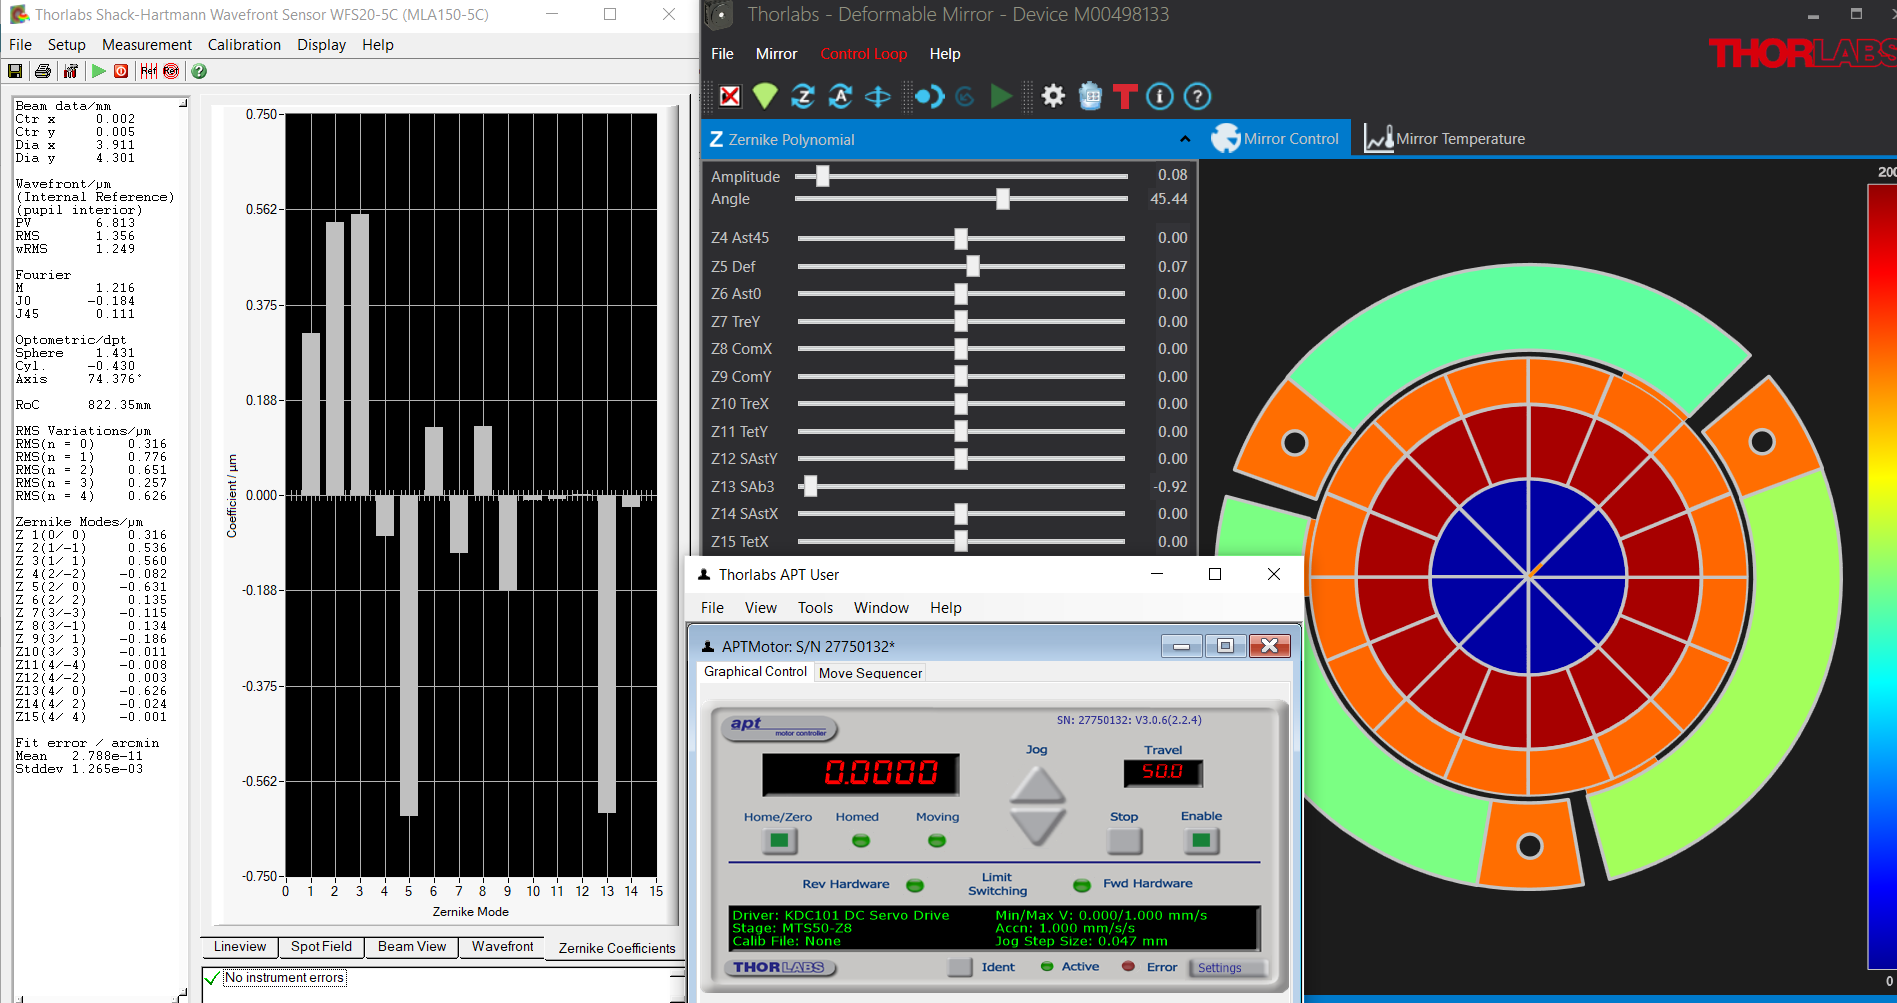
\includegraphics[width=0.95\linewidth]{cap5-eval3-fig1-setup-thorlabs.png}
  \caption{Estado inicial del experimento para la tercera evaluación, capturado desde la
  interfaz en vivo del software del fabricante (\textit{WFS Series Wavefront Analysis
  Software}, Thorlabs) en la posición central $\sigma=0$. La pestaña de control del espejo
  deformable muestra el modo $Z_{13}$ \textit{SAb3} en su valor negativo, configuración
  nominalmente igual a la utilizada en la segunda evaluación
  (Sección~\ref{sec:eval-z13-m1n2}), con el deslizador en $-0.92$; la ventana del
  controlador del servomotor (Thorlabs APT, MTS50-Z8) reporta el paso programado de
  $0.047$~mm correspondiente a la nueva dirección $(m,n)=(1,3)$. Esta figura se incluye
  como referencia del estado experimental; no se utiliza en el análisis cuantitativo.}
  \label{fig:cap5-eval3-fig1}
\end{figure}

Como en la segunda evaluación, la región sobre la que el software del fabricante entrega
su reconstrucción es notablemente menor que la región sobre la que el sensor registra
centroides válidos. La Fig.~\ref{fig:cap5-eval3-fig6} ilustra esta diferencia: el panel
\textbf{a)} muestra los centroides medidos en la toma central $\sigma=0$ tal como los
entrega el sensor, mientras que el panel \textbf{b)} muestra únicamente los puntos del
mallado de salida que el software del fabricante reconstruye. La consideración es la misma
que se discutió en la sección anterior: la comparación cuantitativa contra Thorlabs queda
restringida al área donde el fabricante reporta datos, y por ese motivo los puntos de
Thorlabs se filtran al mismo radio $R$ antes del emparejamiento por vecino más cercano.

\begin{figure}[htbp]
  \centering
  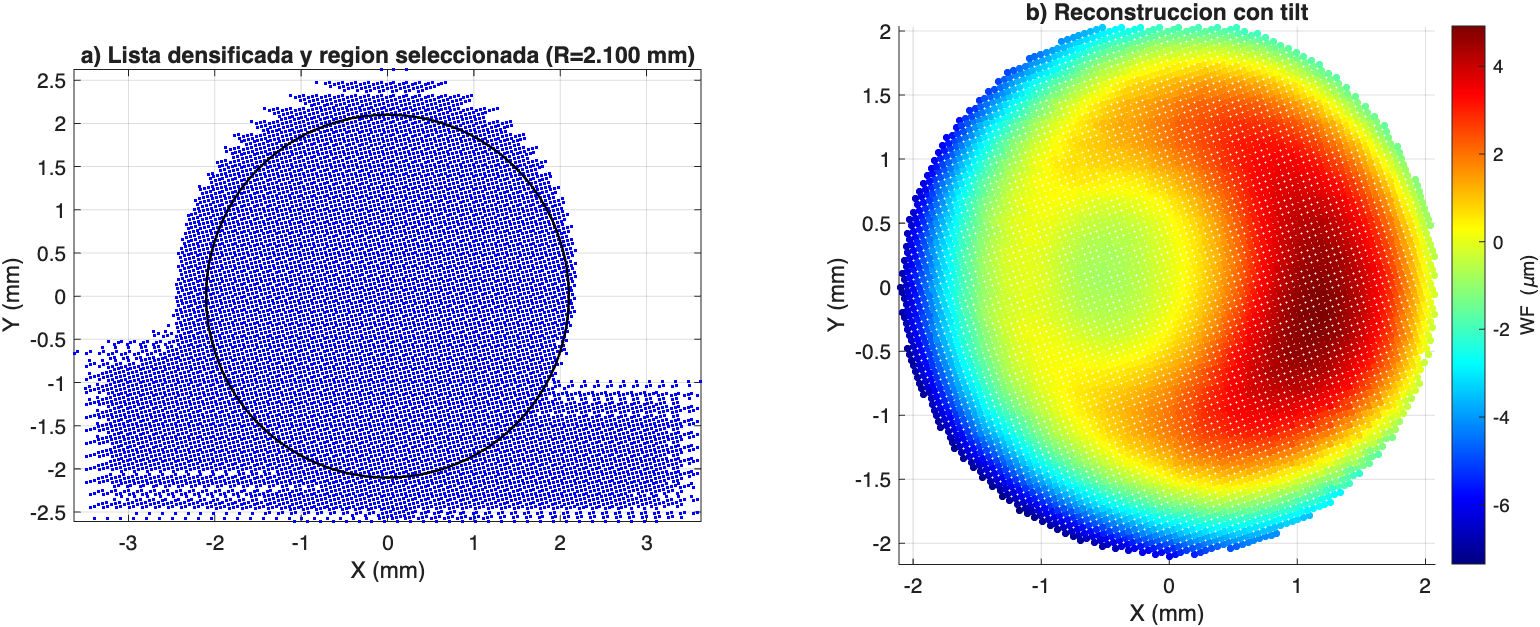
\includegraphics[width=\linewidth]{cap5-eval3-fig2-seleccion-recon-tilt.png}
  \caption{\textbf{a)} Lista densificada de centroides obtenida por composición de los
  diez corrimientos en la dirección $(m,n)=(1,3)$, con la frontera circular de radio
  $R=2.10$~mm superpuesta. \textbf{b)} Reconstrucción inicial del frente de onda en vista
  cenital, todavía con tip, tilt y pistón residuales; el color codifica la altura del
  frente de onda reconstruido en cada centro de microlente.}
  \label{fig:cap5-eval3-fig2}
\end{figure}

A partir de los datos así seleccionados, se aplica la remoción de tip, tilt y pistón a
cada frente de onda por mínimos cuadrados y, a continuación, el segundo tratamiento
descrito en la Sección~\ref{sec:eval2-segundo-tratamiento} para alinear los planos
residuales entre las dos reconstrucciones. Las condiciones que motivaron este segundo paso
en la evaluación anterior se mantienen aquí (diferencia entre dominios de muestreo, con
$6154$ puntos en la lista densificada frente a $501$ puntos canónicos del fabricante), por
lo que el procedimiento se aplica directamente sin replicar el análisis de descubrimiento.
La Fig.~\ref{fig:cap5-eval3-fig3} muestra el resultado final como nube de puntos en cuatro
vistas: la fila superior presenta la perspectiva completa (puntos canónicos del fabricante
y puntos densificados del método de corrimiento), y la fila inferior un acercamiento sobre
una región acotada de la pupila para hacer evidente el incremento en la densidad de
muestreo aportado por el factor $\varepsilon=10$.

La misma reconstrucción puede representarse como superficie triangulada para evidenciar la
continuidad del frente de onda reconstruido. La Fig.~\ref{fig:cap5-eval3-fig5} muestra el
resultado, donde ambos frentes de onda presentan la misma forma global asociada al modo
esférico $Z_{13}$ y la diferencia en densidad de la triangulación refleja directamente el
factor $\varepsilon=10$.

\begin{figure}[htbp]
  \centering
  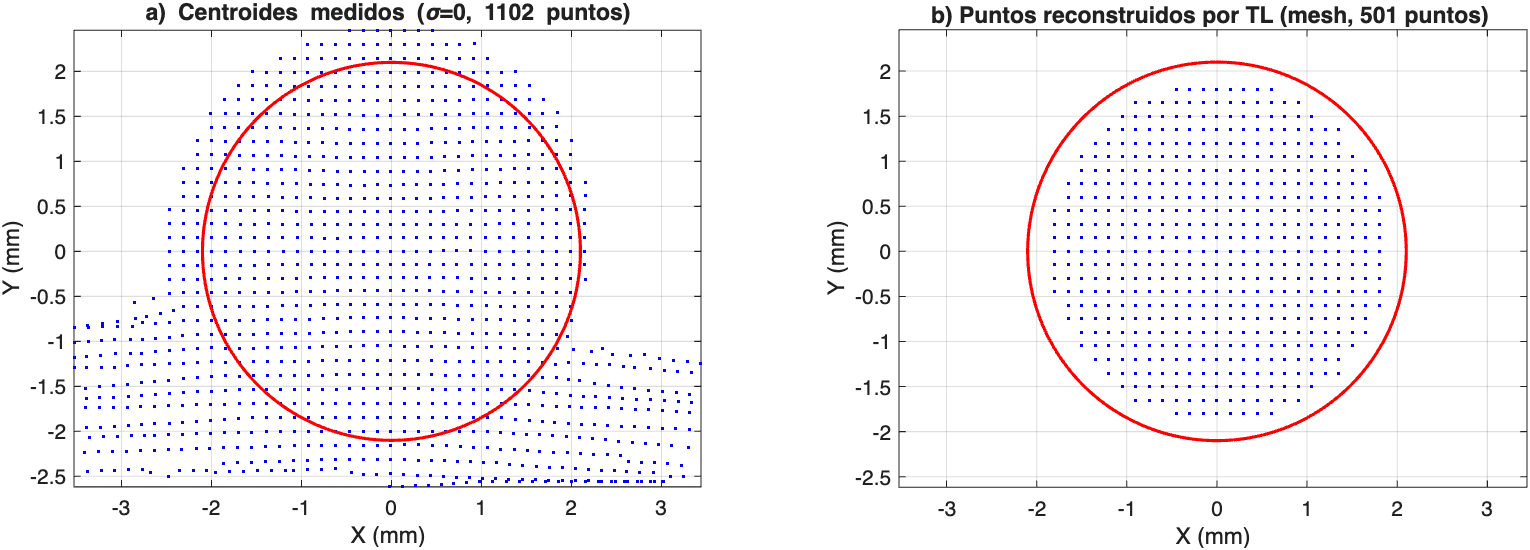
\includegraphics[width=\linewidth]{cap5-eval3-fig6-centroides-vs-mesh-tl.png}
  \caption{Comparación entre los centroides medidos por el sensor y los puntos que el
  software del fabricante reconstruye en la tercera evaluación. \textbf{a)} Centroides
  extraídos de la toma central $\sigma=0$, con la frontera circular de radio $R$
  superpuesta. \textbf{b)} Puntos del mallado de salida que Thorlabs entrega en su archivo
  de reconstrucción, con la misma frontera. El subconjunto reconstruido es notablemente
  más pequeño que el conjunto de centroides medidos.}
  \label{fig:cap5-eval3-fig6}
\end{figure}

\begin{figure}[htbp]
  \centering
  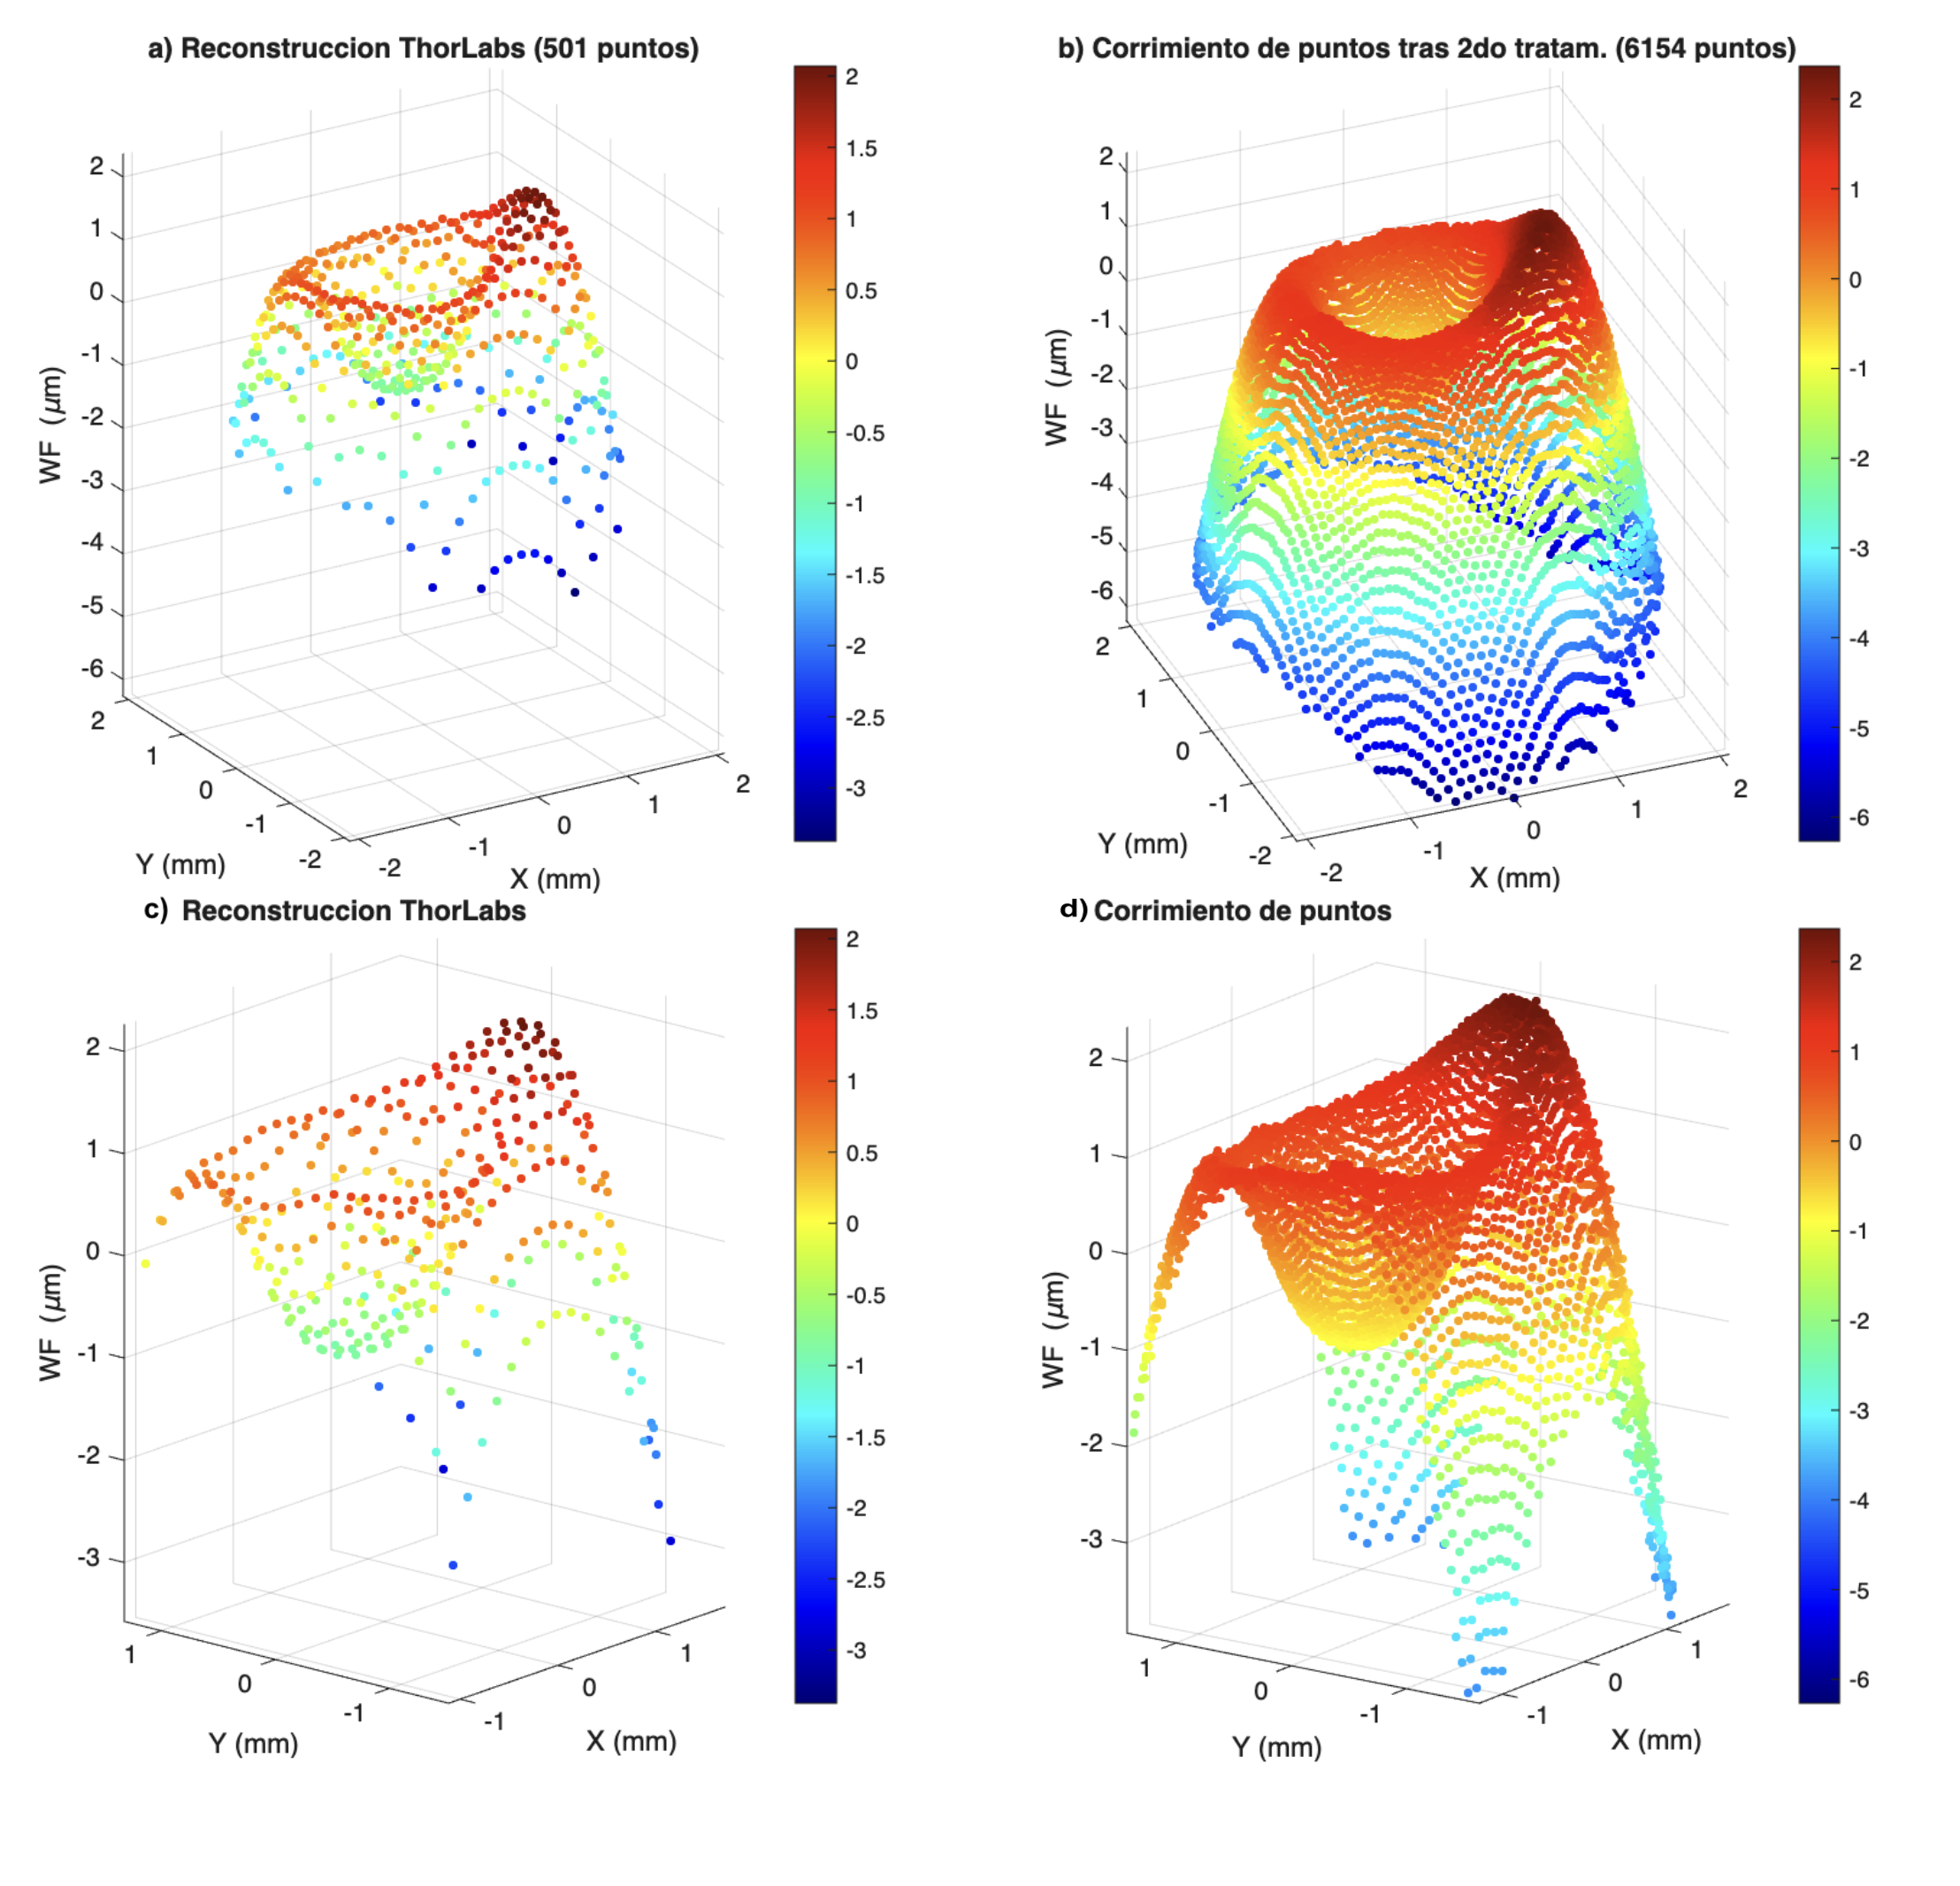
\includegraphics[width=\linewidth]{cap5-eval3-scatter-perspectiva-acercamiento.png}
  \caption{Reconstrucción del frente de onda como nube de puntos tras la remoción de tip,
  tilt y pistón y la aplicación del segundo tratamiento descrito en la
  Sección~\ref{sec:eval2-segundo-tratamiento}. Fila superior, vista en perspectiva
  completa: \textbf{a)} Thorlabs ($501$ puntos canónicos), \textbf{b)} corrimiento de
  puntos sobre la lista densificada ($6154$ puntos). Fila inferior, acercamiento a una
  región acotada de la pupila: \textbf{c)} Thorlabs (paso $0.150$~mm), \textbf{d)}
  corrimiento de puntos (paso efectivo $0.150/\sqrt{10} \approx 0.047$~mm). El factor
  $\varepsilon=10$ se aprecia directamente como aumento de densidad entre los paneles del
  fabricante y los del método propuesto.}
  \label{fig:cap5-eval3-fig3}
\end{figure}

\begin{figure}[htbp]
  \centering
  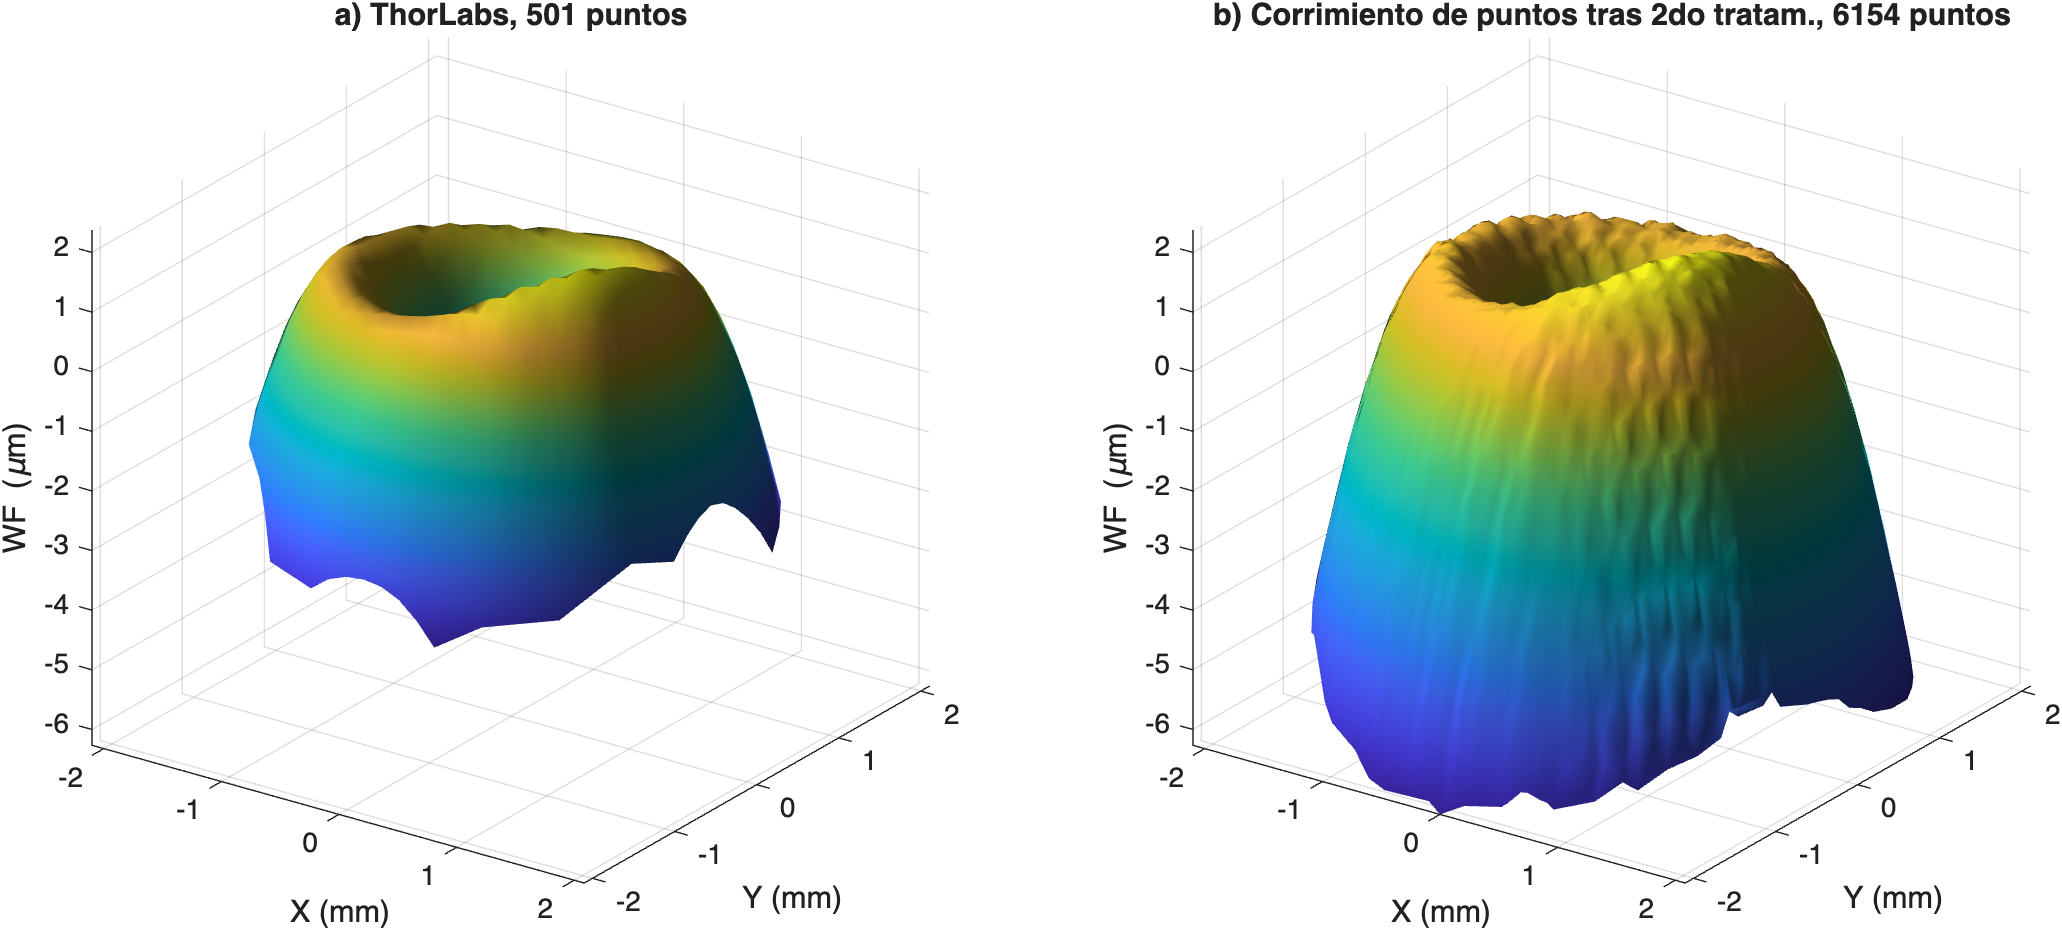
\includegraphics[width=\linewidth]{cap5-eval3-trisurf-sin-ttp.png}
  \caption{Reconstrucción del frente de onda como superficie triangulada (Delaunay), tras
  la aplicación del segundo tratamiento. \textbf{a)} Thorlabs sobre el arreglo canónico de
  microlentes ($501$ puntos, paso $0.150$~mm). \textbf{b)} Reconstrucción por el método de
  corrimiento de puntos sobre la lista densificada ($6154$ puntos, paso efectivo
  $0.150/\sqrt{10} \approx 0.047$~mm). Ambas superficies presentan la misma forma global
  asociada al modo esférico $Z_{13}$; la diferencia en densidad de la triangulación entre
  paneles refleja directamente el factor $\varepsilon=10$. Las escalas verticales de los
  paneles no coinciden porque los dominios difieren: el fabricante entrega su
  reconstrucción sólo en la región central, mientras que la lista densificada se extiende
  hasta el radio de selección $R$, donde la aberración esférica alcanza valores mayores.}
  \label{fig:cap5-eval3-fig5}
\end{figure}

\subsection{Resumen cuantitativo de la tercera evaluación}\label{sec:z13-m1n3-tabla-resumen}

La Tabla~\ref{tab:cap5-resumen-eval3} concentra los parámetros geométricos, los planos
restados a cada reconstrucción y las tres métricas de fidelidad obtenidas en orden de
procesado.

\begin{table}[htbp]
\centering
\caption{Resumen cuantitativo de la tercera evaluación: dirección $(m,n)=(1,3)$,
aberración $Z_{13}$ (esférica primaria), amplitud relativa del software $-0.92$.}
\label{tab:cap5-resumen-eval3}
\small
\begin{tabularx}{\textwidth}{>{\raggedright\arraybackslash}Xl}
\hline
\textbf{Cantidad} & \textbf{Valor} \\
\hline
Puntos reconstruidos (lista densificada) & $6154$ \\
Puntos canónicos (referencia Thorlabs)   & $501$ \\
Caminos de integración depurados         & $1477$ \\
Radio de selección $R$                   & $2.10$~mm \\
Cota de vecindad                         & $0.0670$~mm \\
\hline
Plano restado, corrimiento de puntos $(a, b, c)$ & $(1.72\times 10^{-3},\ 3.82\times 10^{-4},\ 1.37\times 10^{-4})$ \\
Plano restado, Thorlabs $(a, b, c)$              & $(6.10\times 10^{-4},\ 6.13\times 10^{-4},\ 7.83\times 10^{-4})$ \\
\hline
RMS diferencia directa                          & $1.12~\mu$m \\
RMS diferencia tras TTP independiente       & $0.71~\mu$m \\
RMS diferencia tras segundo tratamiento     & $0.13~\mu$m \\
\hline
\end{tabularx}
\end{table}

\section{Análisis de los resultados obtenidos hasta este punto}\label{sec:cap5-analisis}

Las tres evaluaciones presentadas en este capítulo permiten formular un análisis sobre el
comportamiento del método de corrimiento de puntos en condiciones de aberración no nula.
La Tabla~\ref{tab:cap5-comparativa-evals} concentra las métricas de fidelidad de las tres
evaluaciones para facilitar la lectura conjunta.

\begin{table}[htbp]
\centering
\caption{Comparativa de las tres evaluaciones reportadas. La fila ``Aberración impuesta''
designa el modo del software de control del espejo deformable que fue activado en cada
evaluación (convención y formas analíticas en la Sección~\ref{sec:convencion-zernike},
Tabla~\ref{tab:modos-dm}), no un coeficiente Zernike calculado sobre la reconstrucción. La
fila ``RMS final'' corresponde a la métrica de fidelidad principal: en la evaluación 1 al
residuo tras el ajuste TTP independiente (el segundo tratamiento resulta innecesario, como
se discute más adelante); en las evaluaciones 2 y 3, al residuo tras el segundo
tratamiento descrito en la Sección~\ref{sec:eval2-segundo-tratamiento}. En las tres
evaluaciones el modo del espejo se activó con amplitud negativa cercana al extremo del
deslizador ($-0.99$, $-0.97$ y $-0.92$ respectivamente, en el intervalo $[-1,+1]$ del
software); las dos últimas comparten el mismo modo ($Z_{13}$) pero distinta dirección de
barrido y factor de densificación.}
\label{tab:cap5-comparativa-evals}
\small
\begin{tabularx}{\textwidth}{>{\raggedright\arraybackslash}X*{3}{>{\centering\arraybackslash}p{60pt}}}
\hline
\textbf{Cantidad} & \textbf{Eval. 1} & \textbf{Eval. 2} & \textbf{Eval. 3} \\
\hline
Dirección $(m,n)$           & $(1,2)$           & $(1,2)$           & $(1,3)$           \\
Factor $\varepsilon$        & $5$               & $5$               & $10$              \\
Aberración impuesta         & $Z_{11}$ (tetrafoil) neg. máx.& $Z_{13}$ (esférica) neg. máx.& $Z_{13}$ (esférica) neg. máx.\\
Puntos reconstruidos        & $2638$            & $3082$            & $6154$            \\
\hline
RMS diferencia directa          & $1.16~\mu$m       & $1.18~\mu$m       & $1.12~\mu$m       \\
RMS diferencia post-TTP     & $0.145~\mu$m      & $0.67~\mu$m       & $0.71~\mu$m       \\
RMS diferencia final        & $0.145~\mu$m      & $0.14~\mu$m       & $0.13~\mu$m       \\
\hline
\end{tabularx}
\end{table}

La lectura conjunta de la columna de RMS final muestra un comportamiento notablemente
uniforme: las tres evaluaciones convergen a residuos del mismo orden de magnitud, todos
comprendidos entre $0.13$ y $0.145~\mu$m, es decir, por debajo de $\lambda/4$ y cercanos a
$\lambda/5$ para la longitud de onda de trabajo (635 nm). Esta consistencia se obtiene a
pesar de que las evaluaciones difieren en la aberración impuesta (modo tetrafoil $Z_{11}$
frente a esférico $Z_{13}$), en la dirección de barrido $(m,n)$ y en el factor de
densificación $\varepsilon$; es decir, el método produce frentes de onda cuya diferencia
respecto a la reconstrucción del fabricante se mantiene estable frente a cambios
sustanciales en la geometría experimental.

El comportamiento por evaluación de la columna RMS post-TTP merece un comentario, porque
entre las evaluaciones 2 y 3 y la 1 hay un salto aparente que el segundo tratamiento
corrige. En las evaluaciones 2 y 3, el ajuste TTP independiente sobre dos dominios de
muestreo distintos deja un pistón residual entre las dos reconstrucciones, según se
analizó en la Sección~\ref{sec:eval2-segundo-tratamiento}; ese pistón incrementa
artificialmente el RMS post-TTP a $0.67$ y $0.71~\mu$m respectivamente. Tras aplicar el
segundo tratamiento (un único plano ajustado a la diferencia), el residuo cae a $0.14$ y
$0.13~\mu$m. En la primera evaluación el segundo tratamiento se aplicó por completitud
pero su efecto es nulo a la precisión disponible: el plano ajustado a la diferencia
post-TTP tiene coeficientes prácticamente cero ($a \approx -2 \times 10^{-5}$, $b \approx
1 \times 10^{-6}$, $c \approx -8$ nm) y la métrica cambia de $0.145$ a $0.144~\mu$m,
dentro del ruido numérico. La magnitud del pistón residual que deja el ajuste TTP
independiente depende de cómo se distribuyen las muestras de cada dominio sobre la pupila
en cada evaluación concreta; en la primera evaluación los planos individuales resultaron
compatibles entre sí, mientras que en la segunda y la tercera no lo fueron, lo que hizo
necesaria la corrección adicional. No se identificó un criterio \emph{a priori} que
permita predecir la magnitud de este sesgo; por esta razón el segundo tratamiento se
aplica de forma sistemática y se reporta su efecto en cada caso, sea despreciable o no.

A partir de la columna de RMS final (la métrica que describe el error real de la
reconstrucción una vez resueltos los sesgos de muestreo) se desprenden las observaciones
que definen el alcance del trabajo realizado hasta aquí.

\subsection{Estabilidad del residuo al variar la dirección y el factor de densificación}\label{sec:analisis-estabilidad}

Al pasar de cinco a diez corrimientos en la misma aberración (evaluaciones 2 y 3), el
número de puntos reconstruidos prácticamente se duplica ($3082 \to 6154$), sin embargo el
RMS final de la diferencia respecto al software del fabricante se mantiene esencialmente
sin cambio: $0.14$ y $0.13~\mu$m respectivamente. La diferencia entre ambos valores ($\sim
10$~nm) está dentro del margen atribuible a las variaciones residuales del montaje al
cambiar la dirección de barrido, ya que esto implica reorientar el goniómetro, reajustar
la altura y reprogramar el paso del servomotor. Es decir, dentro del rango cubierto por
las evaluaciones, el incremento del factor de densificación no se traduce en una pérdida
ni en una ganancia cuantificable de fidelidad punto a punto: la densidad aumenta de forma
proporcional a $\varepsilon$, el residuo no.

Esta estabilidad cuantitativa, observada en el régimen experimental cubierto por las dos
evaluaciones (mismo espejo deformable, misma aberración impuesta, distintas direcciones y
factores de densificación), resulta coherente con el carácter del método de corrimiento de
puntos como un re-muestreo espacial sobre el mismo arreglo físico de microlentes: la
densificación incrementa el número de muestras del mismo frente de onda sin modificar la
precisión angular de cada medida individual. Lo que se espera de los datos reales
adicionales no es un menor residuo, sino que la información permita conocer más detalles
del frente de onda; en otros términos, que se evalúen mayores frecuencias espaciales del
frente de onda (véase la Sección~\ref{sec:trabajo-futuro}). Determinar si la estabilidad
observada se mantiene en regímenes con aberraciones de mayor curvatura, factores de
densificación más allá de los aquí evaluados o métodos de integración alternativos
requiere experimentos adicionales que quedan fuera del alcance de este trabajo.

\subsection{Posición del método respecto a la reconstrucción del fabricante}\label{sec:analisis-vs-fabricante}

Por construcción, la métrica de fidelidad reportada en este trabajo es la diferencia
respecto a la reconstrucción que el software del fabricante entrega sobre los mismos
centroides medidos. Esta elección no implica que la reconstrucción del fabricante sea
exacta: la propia documentación del sensor reconoce un margen de error en el algoritmo
modal que utiliza, y los puntos del mallado de salida sobre los que reporta sus alturas no
son uniformes en densidad ni cubren la misma área que los centroides registrados, según se
ilustró en la Sección~\ref{sec:eval-z13-m1n2} y siguientes. La afirmación que sí queda
sostenida es doble. Primero, la fidelidad: las reconstrucciones obtenidas por el método de
corrimiento de puntos difieren de la referencia del fabricante en menos de $0.15~\mu$m RMS
tras el tratamiento completo (una discrepancia directamente submicrométrica, inferior a
$\lambda/4$ y muy por debajo de la magnitud de las aberraciones impuestas), estable frente
a cambios en la dirección de barrido y el factor de densificación. Segundo, el contenido
de información: sobre esa base de acuerdo mutuo, la reconstrucción del método contiene
aproximadamente $\varepsilon$ veces más puntos medidos que la del fabricante y cubre una
región igual o mayor que la que este reporta. En este sentido, la conjetura de este
trabajo es que la reconstrucción obtenida constituye una \emph{mejor medida} del frente de
onda: no porque cada punto individual sea más exacto que el del fabricante (eso no puede
establecerse con una métrica relativa), sino porque, a igualdad de fidelidad demostrada,
describe visualmente el mismo frente de onda con un muestreo real más denso; el acceso a
estructura espacial que la malla canónica no puede representar es la expectativa que de
ello se deriva, no verificada en este trabajo. Confirmar esta conjetura en términos
absolutos requiere la validación contra una referencia independiente que se discute en el
Capítulo~\ref{cap:conclusiones}. No se afirma una mejora punto a punto sobre el
fabricante; tampoco se asume que el fabricante esté libre de error.

\subsection{Aumento de resolución espacial e implicaciones para extensiones futuras}\label{sec:analisis-resolucion}

El producto principal del método, frente a la reconstrucción del fabricante, es el aumento
del número de puntos sobre los que se entrega el frente de onda: en las tres evaluaciones,
el factor entre los puntos de la lista densificada y los puntos canónicos del fabricante
coincide aproximadamente con el factor $\varepsilon$ teórico ($2638/501 \approx 5.3$,
$3082/503 \approx 6.1$, $6154/501 \approx 12.3$, los desbalances respecto a $\varepsilon$
exacto se deben al recorte circular y a la región sobre la que el fabricante reporta
datos). Este incremento se obtiene sin modificar la geometría del arreglo de microlentes
y, por tanto, el rango dinámico angular por microlente $\alpha_{max}=P_L/(2f_L)$ se
conserva por construcción al ser idénticos el paso $P_L$ y la distancia focal $f_L$ entre
las tres evaluaciones y la reconstrucción del fabricante. Disminuir el compromiso entre
densidad de muestreo y rango dinámico es la propuesta metodológica original de la técnica.

Hay que subrayar la naturaleza de los puntos adicionales que el método aporta. La lista
densificada no se obtiene por interpolación de los datos canónicos: cada centroide
adicional corresponde a una medida experimental directa, extraída de uno de los
$\varepsilon$ spotgramas adquiridos en posiciones de barrido distintas. El método entrega,
por tanto, información real del frente de onda en posiciones intermedias entre los centros
del arreglo de microlentes, no estimaciones obtenidas a partir de los vecinos. La
triangulación que se utiliza en las superficies presentadas
(Figs.~\ref{fig:cap5-fig5-6-1}, \ref{fig:cap5-eval2-fig6} y \ref{fig:cap5-eval3-fig5})
únicamente conecta esos puntos para visualizarlos como superficie continua, sin generar
contenido nuevo entre ellos.

La integración numérica empleada (regla del trapecio sobre caminos voraces) se escogió
deliberadamente como la opción más simple disponible, para que el residuo cuantificado
refleje predominantemente la calidad de los datos y la consistencia del procedimiento
experimental, no la sofisticación del integrador. Esta elección tiene una consecuencia que
hay que anotar: el integrador trapezoidal opera sobre trayectorias unidimensionales
sucesivas y no aprovecha simultáneamente toda la densidad disponible en la lista
densificada en todas las direcciones de la pupila. Métodos de reconstrucción zonal o
ajustes locales con información adicional, que sí podrían beneficiarse de la cobertura
completa, quedan fuera del alcance del trabajo presente y se dejan como continuación
natural.

Por último, los resultados aquí reportados están sujetos a las precisiones del control
mecánico del montaje (resolución angular del goniómetro y de la platina AP180,
repetibilidad bidireccional del servomotor); la propagación cuantitativa de estas fuentes
de error a la métrica de fidelidad no se ha realizado en este trabajo y se retoma como
línea de trabajo futuro en la Sección~\ref{sec:trabajo-futuro}.


\chapter{Conclusiones}\label{cap:conclusiones}

A partir de las tres evaluaciones experimentales documentadas en el
Capítulo~\ref{cap:resultados} y del análisis presentado en la
Sección~\ref{sec:cap5-analisis}, se establecen los resultados puntuales que sostienen el
alcance del trabajo realizado.

\paragraph{Ganancia neta del método.} Con el mismo sensor, sin componentes ópticos
adicionales y con un solo eje de traslación durante el barrido (la rotación del sensor
sólo selecciona la dirección y se fija antes de medir), se obtiene un muestreo del frente
de onda $\varepsilon$ veces más denso, compuesto por mediciones reales y no por
interpolaciones, conservando por construcción el rango dinámico del arreglo de
microlentes. El costo es adquirir $\varepsilon$ imágenes en lugar de una y procesarlas en
conjunto. Se espera además que esto dé acceso a frecuencias espaciales del frente de onda
que el arreglo canónico no alcanza a muestrear, contenido que no se midió en este trabajo.

\paragraph{Comparabilidad cuantitativa con la reconstrucción del fabricante.} El método de
corrimiento de puntos, implementado con la integración numérica más simple disponible
(regla del trapecio sobre caminos voraces), produce reconstrucciones cuya diferencia RMS
respecto al software del fabricante (una vez resueltos los sesgos de muestreo mediante el
ajuste TTP independiente y, cuando las condiciones del experimento lo requieren, el
segundo tratamiento descrito en la Sección~\ref{sec:eval2-segundo-tratamiento}) queda en
las tres evaluaciones por debajo de $0.15~\mu$m, esto es, por debajo de $\lambda/4$ para
la longitud de onda de trabajo (635 nm) (Tabla~\ref{tab:cap5-comparativa-evals}). La
afirmación es relativa, no absoluta: no se sostiene una mejora sobre el fabricante ni se
asume que la reconstrucción del fabricante sea exacta; lo que se valida es que el método
arroja resultados \emph{comparables} a los del fabricante sobre las mismas mediciones, con
un residuo del mismo orden en todas las configuraciones experimentales evaluadas.

\paragraph{Aumento de resolución espacial mediante observaciones reales.} La lista
densificada producida por el método contiene, en las tres evaluaciones reportadas, un
número de puntos aproximadamente igual al factor $\varepsilon = m^2 + n^2$ veces el de la
reconstrucción del fabricante sobre la misma región: factores cercanos a cinco para las
dos primeras evaluaciones ($\varepsilon=5$) y a diez para la tercera ($\varepsilon=10$).
Cada uno de los puntos adicionales corresponde a un centroide medido directamente sobre
uno de los $\varepsilon$ spotgramas adquiridos, no a una estimación obtenida por
interpolación de los datos canónicos: el método entrega información experimental real del
frente de onda en posiciones intermedias entre los centros del arreglo de microlentes. La
triangulación que se utiliza en las visualizaciones tridimensionales únicamente conecta
esos puntos para representarlos como superficie continua, sin generar contenido nuevo
entre ellos.

\paragraph{Preservación del rango dinámico por construcción.} El paso $P_L$ y la distancia
focal $f_L$ del arreglo de microlentes son idénticos en las tres evaluaciones y en la
reconstrucción del fabricante; en consecuencia, el rango dinámico angular por microlente
$\alpha_{max}=P_L/(2f_L)$ se conserva por construcción al no modificarse ningún elemento
físico del sensor. La consistencia experimental observada entre las tres evaluaciones, con
residuos contra el fabricante en el mismo orden de magnitud y por debajo de $\lambda/4$
visible, sostiene que el aumento de la densidad de muestreo no se obtiene a costa del
rango dinámico ni introduce un sesgo cuantificable adicional sobre la fidelidad de la
reconstrucción.

\paragraph{Identificación de un pistón residual en la remoción TTP independiente sobre
dominios asimétricos.} Durante el análisis de la segunda evaluación se identificó que el
ajuste de plano por mínimos cuadrados aplicado a cada frente de onda por separado no
garantiza la cancelación del pistón relativo entre las dos reconstrucciones cuando los
dominios sobre los que se calculan los planos tienen densidades de muestreo distintas
(Sección~\ref{sec:eval2-segundo-tratamiento}). El sesgo introducido es directamente
atribuible al procedimiento de remoción de modos bajos y no al frente de onda físico bajo
prueba. Para eliminarlo es suficiente con ajustar un único plano a la diferencia entre
ambas reconstrucciones y restarlo, procedimiento que resulta algebraicamente equivalente a
corregir cualquiera de los dos frentes de onda con ese mismo plano. Este resultado,
identificado y caracterizado durante el desarrollo del trabajo, es de aplicación general
en comparaciones cuantitativas entre frentes de onda reconstruidos sobre dominios
espaciales distintos y constituye un aporte metodológico que excede el caso particular del
método de corrimiento de puntos.

\paragraph{Estabilidad del residuo en el régimen experimental cubierto.} En el rango de
configuraciones evaluadas (factores de densificación $\varepsilon=5$ y $\varepsilon=10$,
aberraciones $Z_{11}$ y $Z_{13}$ impuestas por el espejo deformable, dos direcciones de
barrido distintas) el residuo final respecto a la reconstrucción del fabricante se
mantiene en el mismo orden de magnitud, sin que el incremento del factor de densificación
se traduzca en una variación cuantificable de la fidelidad punto a punto. Esta estabilidad
debe leerse junto con la naturaleza de la ganancia del método: lo que se espera del
aumento de datos reales medidos no es una reducción del residuo respecto a la referencia,
sino que la información adicional permita conocer más detalles del frente de onda, en
otros términos, evaluar mayores frecuencias espaciales del frente de onda, contenido que
la métrica RMS punto a punto aquí empleada, calculada sobre la región común a ambas
reconstrucciones, no está diseñada para capturar. Determinar si esta estabilidad se
mantiene en regímenes con aberraciones de mayor curvatura, factores de densificación más
allá de los aquí evaluados o métodos de integración alternativos, así como cuantificar el
contenido de frecuencias espaciales efectivamente recuperado, requiere experimentos
adicionales que quedan fuera del alcance del presente trabajo. Sería deseable abordarlos
en un trabajo posterior.

\paragraph{Limitaciones y costo del método.} La limitación principal es que sólo sirve
para frentes de onda que no cambien durante las $\varepsilon$ capturas: la composición de
los corrimientos supone un único frente de onda estático
(Sección~\ref{sec:composicion-corrimientos}). Al costo de las $\varepsilon$ imágenes ya
señalado se suman tiempo y complejidad del arreglo. El método del fabricante requiere una
sola captura y reconstruye en vivo. Tal como se implementó, el corrimiento de puntos es un
prototipo con secuencia manual de desplazamiento y captura: con el montaje listo y el
frente inmóvil, cada captura toma unos 30 segundos, de modo que un barrido completo
requiere del orden de $30\,\mathrm{s}\times\varepsilon$, entre dos y tres minutos para
$\varepsilon=5$ y unos cinco para $\varepsilon=10$ (estimación del autor, no medida), sin
contar el armado del experimento; el procesamiento posterior, una vez desarrollado el
código, toma unos segundos. Un sistema semiautomatizado podría completar las $\varepsilon$
capturas en pocos segundos, pero aun así exigiría un frente de onda estable durante ese
lapso. Además requiere el sistema de posicionamiento y control del Capítulo~3, que el
fabricante no necesita. Eso es un costo real. La rotación que fija el ángulo, el reajuste
de altura que la acompaña y la inclinación del sensor se fijan antes del barrido
(Sección~\ref{sec:ajuste-angulo}); durante la medición sólo se mueve la platina de
desplazamiento. Ese ajuste y el paso de cada corrimiento son fuentes de error que una sola
imagen no tiene, y el análisis añade dos etapas: la composición de las $\varepsilon$
listas y la selección de la región útil (Sección~\ref{sec:seleccion-region}). No se
propagaron ni se separaron de las demás contribuciones al residuo; la única cifra que las
contiene es la diferencia total frente al fabricante tras el tratamiento completo
(Tabla~\ref{tab:cap5-comparativa-evals}). Ni la precisión absoluta del método ni su
repetibilidad se midieron: la única cifra de precisión disponible es la que el catálogo
declara para el sensor con su software, $\lambda/30$ RMS (Tabla~\ref{tab:ap-wfs}), no
verificada aquí, y lo medido en este trabajo es la diferencia entre ambas
reconstrucciones. La alineación inicial es un centrado visual sin referencia absoluta
(Sección~\ref{sec:alineacion-sistema}), así que dos evaluaciones no muestrean exactamente
las mismas posiciones; que sus reconstrucciones coincidan salvo una traslación es
conjetura no probada (Sección~\ref{sec:trabajo-futuro}). En los mapas de diferencia el
residuo tiende a crecer hacia el borde de la región
(Fig.~\ref{fig:cap5-eval2-diferencias-tres-etapas}\,c); promediar reconstrucciones
obtenidas desde distintos puntos de partida de la integración podría reducirlo, a costa de
un proceso más laborioso que no se intentó.

\paragraph{Cuándo conviene cada método.} Queda establecido que se obtienen $\varepsilon$
veces más puntos medidos con el mismo sensor y rango dinámico, y una diferencia respecto
al fabricante por debajo de $0.15~\mu$m RMS; en las superficies trianguladas las
transiciones de la reconstrucción densificada son visualmente más suaves y detalladas que
las de la malla del fabricante. Que esas muestras den acceso a frecuencias espaciales más
altas se apoya sólo en que se miden más puntos reales en la misma región; es una
predicción razonada, no un resultado: ese contenido no se midió en este trabajo. Tampoco
puede decidirse si un detalle que aparece sólo en la lista densificada es del frente de
onda o un error del método: la métrica RMS sobre la región común no lo captura
(Sección~\ref{sec:diferencia}); esa distinción requiere la referencia independiente
propuesta en la Sección~\ref{sec:trabajo-futuro}. El método del fabricante es el adecuado
cuando la malla canónica basta o cuando el frente de onda cambia en el tiempo; el
corrimiento de puntos conviene cuando se necesita más muestreo espacial de un frente
estable y se dispone del montaje mecánico.

\section{Trabajo futuro y perspectivas}\label{sec:trabajo-futuro}

Las líneas de continuación natural derivadas del trabajo aquí presentado se concentran en
cuatro direcciones.

\paragraph{Propagación cuantitativa del error instrumental.} Los resultados aquí
reportados están sujetos a las precisiones del control mecánico del montaje: el ajuste del
ángulo del sensor depende de la resolución del goniómetro y de la platina AP180
(Sección~\ref{sec:control-desplazamiento-altura}), y el paso de cada corrimiento depende
de la repetibilidad bidireccional del servomotor. La propagación cuantitativa del error
introducido por estas dos fuentes a la métrica de fidelidad reportada no se ha realizado
en este trabajo y es necesaria para acotar el piso de incertidumbre instrumental del
residuo de $\sim 0.13$--$0.15~\mu$m observado en las evaluaciones aberradas. Tampoco se
estudió la repetibilidad de una evaluación completa repetida desde la alineación inicial;
es de esperar que una nueva alineación produzca el mismo frente de onda reconstruido salvo
una traslación espacial, pero esta conjetura no fue puesta a prueba.

\paragraph{Métodos de reconstrucción más sofisticados.} La integración por la regla del
trapecio sobre caminos voraces (un método simple y confiable) fue escogida como la opción
más sencilla disponible para que el residuo cuantificado refleje la calidad de los datos y
no la del integrador. La densidad y la cobertura de la lista densificada son, sin embargo,
suficientes para alimentar reconstrucciones zonales, ajustes locales o esquemas de
interpolación con información adicional que sí podrían aprovechar simultáneamente toda la
información del muestreo en todas las direcciones de la pupila. Explorar este camino,
comparando el residuo obtenido con cada esquema de reconstrucción frente al ya reportado,
es una línea natural de continuación.

\paragraph{Validación contra una referencia distinta a la del fabricante.} Los datos de
este trabajo no permiten establecer cuál de las dos reconstrucciones (la del método de
corrimiento de puntos o la del fabricante) es más confiable en términos absolutos: la
métrica empleada es relativa y ambas reconstrucciones comparten la misma cadena de
medición (mismo sensor, mismo haz, mismos centroides), por lo que sus errores comunes se
cancelan parcialmente al compararlas. La métrica de fidelidad reportada en este trabajo se
construye contra la reconstrucción que entrega el software del fabricante sobre las mismas
mediciones; esta elección hace que la validación quede acotada por la propia incertidumbre
del algoritmo del fabricante. Una validación cruzada contra una referencia independiente
(por ejemplo, una simulación numérica del mismo frente de onda con los parámetros
experimentales medidos, o una caracterización interferométrica del espejo deformable)
permitiría desacoplar la calidad del método de corrimiento de puntos de la del software de
referencia y constituye una extensión deseable del análisis cuantitativo.

\paragraph{Medición de una superficie calibrada.} Las evaluaciones de este trabajo emplean
el espejo deformable como generador de frentes de onda repetibles pero no conocidos en
sentido absoluto (Sección~\ref{sec:sistema-optico}), y, aun con la compensación de
histéresis por software del controlador (Capítulo 3), la respuesta del espejo está sujeta
a efectos de histéresis residual y relajación propios de los actuadores piezoeléctricos,
de modo que la forma real del espejo no se conoce con exactitud. Medir una superficie
calibrada de forma conocida (un elemento óptico certificado en lugar del espejo
deformable) permitiría una validación absoluta del método, independiente tanto del
software de referencia como de la incertidumbre en la forma que el espejo realmente
adopta.

\appendix

\chapter{Disponibilidad de datos y código}\label{ap:disponibilidad}

El código MATLAB que implementa el método de corrimiento de puntos descrito en el
Capítulo~\ref{cap:metodologia}, junto con los datos experimentales originales y las
copias de trabajo utilizadas en las tres evaluaciones del
Capítulo~\ref{cap:resultados}, se encuentran en el siguiente repositorio público:

\begin{center}
\texttt{https://github.com/jz-VEC/shack-hartmann-point-shifting}
\end{center}

\paragraph{Estructura del repositorio.}
\begin{itemize}
\item \texttt{scripts/} --- código MATLAB del método, organizado en \texttt{functions/} (rutinas reutilizables), \texttt{config/} (gestión de rutas) y \texttt{evaluations/}. Este último contiene exclusivamente las evaluaciones \path{m1n2_z11_neg_max}, \path{m1n2_z13_neg_max} y \path{m1n3_z13_max} reportadas en el Capítulo~\ref{cap:resultados}.
\item \texttt{scripts/CONVENTIONS.md} --- documento de referencia con las convenciones de variables (centroides medidos frente a centros geométricos de microlente, estructura por columnas de la matriz de trabajo, métricas RMS, fórmula de la cota de vecindad).
\item \texttt{rawData/} --- datos experimentales originales de las tres evaluaciones, conservados con los nombres y la organización producidos durante la adquisición. La correspondencia entre esos directorios y los nombres normalizados de las evaluaciones se documenta en \texttt{DATA\_MANIFEST.md}.
\item \texttt{data/} --- copias de trabajo completas de los tres datasets, incluidos los CSV de centroides, las retículas de puntos (\textit{mesh}), los registros de potencia y los spotgramas; \texttt{DATA\_MANIFEST.md} identifica los 23 CSV consumidos directamente por los scripts.
\item \texttt{thesis/} --- fuente \LaTeX{} y figuras necesarias para compilar el presente documento. La versión pública excluye la firma del director y otros materiales administrativos.
\end{itemize}

\paragraph{Reproducibilidad de las evaluaciones.} Cada subdirectorio bajo \path{scripts/evaluations/} contiene un script principal con el mismo nombre que reproduce la totalidad del pipeline para ese dataset: lectura de los CSV, aplicación de los corrimientos, concatenación, recorte circular, generación de caminos de integración, integración por la regla del trapecio, eliminación de \textit{tip}, \textit{tilt} y pistón, y, cuando corresponde, el segundo tratamiento descrito en la Sección~\ref{sec:segundo-tratamiento}. La ejecución de los scripts \path{m1n2_z11_neg_max.m}, \path{m1n2_z13_neg_max.m} y \path{m1n3_z13_max.m} regenera las figuras y las métricas RMS reportadas en el Capítulo~\ref{cap:resultados}. Los archivos \texttt{README.md}, \texttt{REPRODUCIBILITY.md} y \texttt{DATA\_MANIFEST.md} de la versión pública especifican los requisitos, comandos y correspondencias de archivos.

\paragraph{Materiales de terceros.} Las imágenes de componentes comerciales y diagramas de
los fabricantes que aparecen en este documento (Thorlabs, Inc.\ y Edmund Optics, Inc.) se
reproducen exclusivamente con fines académicos, sin fin de lucro, con el crédito
correspondiente indicado en el pie de cada figura, en los términos del artículo 148 de la
Ley Federal del Derecho de Autor. Las capturas de pantalla del \textit{WFS Series
Wavefront Analysis Software} y del software de control del espejo deformable corresponden
a sesiones de trabajo del propio experimento. Los derechos sobre las imágenes de los
fabricantes pertenecen a sus respectivos titulares.

\paragraph{Licencia.} El repositorio se distribuye actualmente bajo \textit{All rights
reserved} (véase el archivo \texttt{LICENSE} en la raíz del repositorio); las citas
académicas breves bajo uso justo están permitidas con acreditación apropiada al autor y a
la UNAM. El régimen de licencia a partir de la publicación pública del repositorio se
determinará en su momento.

\chapter[Especificaciones del hardware]{Especificaciones consolidadas del hardware}\label{ap:hardware}

Este apéndice agrupa en formato de tabla las especificaciones técnicas de los componentes
utilizados en el arreglo experimental descrito en el Capítulo~\ref{cap:metodologia}. Los
valores reportados son los declarados por los fabricantes en los respectivos manuales y
catálogos.

\begin{table}[htbp]
\centering
\caption{Sensor Shack-Hartmann Thorlabs WFS20-5C (incluye arreglo de microlentes MLA150-5C).}
\label{tab:ap-wfs}
\begin{tabularx}{\textwidth}{>{\raggedright\arraybackslash}X l}
\hline
\textbf{Parámetro} & \textbf{Valor} \\
\hline
Resolución del sensor CMOS & $1440 \times 1080$ píxeles \\
Área sensible & $7.20 \times 5.40$ mm \\
Tamaño de píxel (cuadrado) & $5\,\mu$m \\
Frecuencia de captura máxima & $1120$ fps \\
Tipo de microlentes & planoconvexas, sílice fundida \\
Distancia focal de las microlentes $f_L$ & $4.1$ mm \\
\textit{Pitch} del arreglo $P_L$ (regular en ambas direcciones) & $150\,\mu$m \\
Precisión del sensor (RMS) & $\lambda/30$ \\
Sensibilidad con software del fabricante (RMS) & $\lambda/100$ \\
\hline
\end{tabularx}
\end{table}

\begin{table}[htbp]
\centering
\caption{Espejo deformable Thorlabs DMP40-FM1.}
\label{tab:ap-dmp40}
\begin{tabularx}{\textwidth}{l >{\raggedright\arraybackslash}X}
\hline
\textbf{Parámetro} & \textbf{Valor} \\
\hline
Tipo de actuador & piezoeléctrico (histéresis compensada por software) \\
Número de actuadores & $40$ \\
Configuración del arreglo de actuadores & circular \\
Distancia de alineación recomendada & $\sim 73$ mm \\
Conectividad con el computador & USB \\
Modos Zernike controlables por software & $Z_4$ a $Z_{15}$ ($12$ términos, Sección~\ref{sec:convencion-zernike}) \\
\hline
\end{tabularx}
\end{table}

\begin{table}[htbp]
\centering
\caption{Subsistema mecánico de posicionamiento y control angular.}
\label{tab:ap-mecanico}
\small
\begin{tabular}{@{}l p{0.55\textwidth}@{}}
\hline
\textbf{Componente} & \textbf{Función y especificaciones} \\
\hline
KM200PM (Thorlabs) & \textit{Ajuste tip-tilt del sensor.} Control fino de inclinación. \\
Goniómetro Edmund Optics 66-526 & \textit{Giro fino del sensor.} Recorrido $\pm 10^\circ$; resolución $5'$ ($\approx 0.08^\circ$). \\
AP180 (Thorlabs) & \textit{Rotación gruesa de ángulo.} Trece posiciones cada $15^\circ$ sobre $180^\circ$; precisión $\pm 18'$ ($\approx \pm 0.3^\circ$). \\
L490 (Thorlabs) & \textit{Mesa de altura variable.} Reajuste de altura del sensor tras cambio de ángulo. \\
MTS50-Z8 (Thorlabs) & \textit{Platina motorizada de translación.} Rango $50$ mm; mínimo movimiento alcanzable $0.05\,\mu$m; incremento mínimo repetible $0.8\,\mu$m; repetibilidad bidireccional $1.6\,\mu$m; carga horizontal recomendada $<10$ kg. \\
KDC101 (Thorlabs) & \textit{Controlador del servomotor.} Software dedicado APT para programar la distancia de cada corrimiento. \\
\hline
\end{tabular}
\end{table}

\begin{table}[htbp]
\centering
\caption{Sistema óptico (kit Thorlabs AOK5/M modificado), fuente de luz y alimentación.}
\label{tab:ap-optico}
\begin{tabularx}{\textwidth}{@{}l >{\raggedright\arraybackslash}X@{}}
\hline
\textbf{Componente} & \textbf{Especificación} \\
\hline
Kit base & Thorlabs AOK5/M, con el espejo deformable original (Multi-DM) sustituido por el DMP40-FM1 (Tabla~\ref{tab:ap-dmp40}). \\
Lente LA1131-B & Distancia focal $50$ mm; forma el foco intermedio del haz sobre el plano de muestra. \\
Lentes LA1608-B & Distancia focal $75$ mm; empleadas para recolimación tras el foco intermedio y en los relevos 4f del diseño del kit (del haz expandido hasta el DM y del haz reflejado hasta el sensor S-H). \\
Espejos PF10-03-P01 & Espejos planos con recubrimiento de plata protegida; alta reflectividad en banda amplia. \\
Divisor de haz BP108 & Película delgada, razón $8{:}92$ (R:T). \\
Caja CBB1 & Cage cube que aloja el plano de muestra (foco intermedio del haz); vacía en este trabajo. \\
Fuente láser & Módulo de diodo láser del kit, $\lambda = 635$ nm, $0.30$ mW (Clase 1). \\
Fuente de alimentación PPT2415 & Alimentación estabilizada compartida por el controlador KDC101 y el sistema de óptica adaptativa. \\
\hline
\end{tabularx}
\end{table}

\chapter{Catálogo de datasets utilizados}\label{ap:datasets}

Las tres evaluaciones experimentales reportadas en el Capítulo~\ref{cap:resultados} se
construyen sobre los datasets resumidos en la Tabla~\ref{tab:ap-datasets}. Cada dataset
corresponde a una configuración fija del sistema (dirección de barrido $(m,n)$ y modo del
espejo deformable) y consiste en $\varepsilon = m^2 + n^2$ archivos CSV de centroides (uno
por corrimiento) exportados por el \textit{WFS Series Wavefront Analysis Software} de
Thorlabs, más un mesh Thorlabs de referencia para la posición central $\sigma = 0$.

\begin{table}[htbp]
\centering
\caption{Datasets utilizados en las tres evaluaciones del Capítulo~\ref{cap:resultados}.
En los tres casos el modo del espejo deformable se activó con amplitud negativa cercana al
extremo del deslizador: $-0.99$, $-0.97$ y $-0.92$ respectivamente
(Sección~\ref{sec:convencion-zernike}).}
\label{tab:ap-datasets}
\small
\begin{tabular}{lcclcl}
\hline
\textbf{Dataset} & $\boldsymbol{(m,n)}$ & $\boldsymbol{\varepsilon}$ & \textbf{Modo DM} & \textbf{\# CSV} & \textbf{Sección} \\
\hline
\texttt{m1n2\_z11\_neg\_max} & $(1,2)$ & $5$  & $Z_{11}$ (tetrafoil) & 5 + mesh  & §\ref{sec:eval-z11-m1n2} \\
\texttt{m1n2\_z13\_neg\_max} & $(1,2)$ & $5$  & $Z_{13}$ (esférica)  & 5 + mesh  & §\ref{sec:eval-z13-m1n2} \\
\texttt{m1n3\_z13\_max}      & $(1,3)$ & $10$ & $Z_{13}$ (esférica)  & 10 + mesh & §\ref{sec:eval-z13-m1n3} \\
\hline
\end{tabular}
\end{table}

\paragraph{Convenciones de los archivos.} Cada archivo de centroides sigue el patrón
\texttt{cent d}$\pm k$\texttt{ }$\pm$\texttt{NNNN.csv}, donde $\pm k$ es el índice entero
del corrimiento (con $k = 0$ para la toma central, sin desplazamiento) y $\pm$NNNN el
desplazamiento físico en micrómetros con signo. El mesh Thorlabs se identifica como
\texttt{mesh d+0 +0000.csv} (con las variantes de \textit{naming} propias de cada dataset
descritas en \texttt{scripts/CONVENTIONS.md}) y contiene la reconstrucción del frente de
onda producida por el software del fabricante, expresada en micrómetros sobre la malla
regular de microlentes.

\paragraph{Modo del espejo deformable.} En los tres datasets, las etiquetas $Z_{11}$ y
$Z_{13}$ designan los modos del software del DMP40-FM1 que fueron activados al límite de
su rango (tetrafoil y esférica primaria respectivamente; convención y formas analíticas en
la Sección~\ref{sec:convencion-zernike}), no coeficientes de Zernike calculados sobre la
reconstrucción. La calibración fina del espejo y la determinación cuantitativa del frente
de onda generado para cada combinación de actuadores queda fuera del alcance de esta tesis
(Sección~\ref{sec:sistema-optico}).


\addcontentsline{toc}{chapter}{Bibliografía}
\begin{thebibliography}{100}
	
	\bibitem{Shack}
	B. C. Platt and R. V. Shack, ``Lenticular Hartmann screen,'' Optical Sciences Center Newsletter (University of Arizona) 5, 15--16 (1971).
	
	\bibitem{PlattShack}
	B. C. Platt and R. V. Shack, ``History and principles of Shack-Hartmann wavefront sensing,'' Journal of Refractive Surgery, Vol. 17, No. 5, pp. S573-S577, 2001. DOI: 10.3928/1081-597X-20010901-13.
	
	\bibitem{Tyson}
	R. K. Tyson, Principles of Adaptive Optics, 3rd ed., CRC Press, 2011.
	
	\bibitem{Hartmann}
	J. Hartmann, ``Bemerkungen über den Bau und die Justirung von Spektrographen,'' Zeitschrift für Instrumentenkunde 20, 47--58 (1900).
	
	\bibitem{Malacara}
	D. Malacara, Optical Shop Testing, 3rd ed., Wiley, 2007.
	
	\bibitem{MalacaraDoblado}
	D. Malacara-Hernández and D. Malacara-Doblado, ``What is a Hartmann test?,'' Appl. Opt. 54(9), 2296--2301 (2015). DOI: 10.1364/AO.54.002296.

	\bibitem{Goodman}
	J. W. Goodman, Introduction to Fourier Optics, 3rd ed., Roberts and Company, 2005.

	\bibitem{AkondiDubra}
	V. Akondi and A. Dubra, ``Shack-Hartmann wavefront sensor optical dynamic range,'' Opt. Express 29(6), 8417--8429 (2021). DOI: 10.1364/OE.419311.

	\bibitem{Greivenkamp}
	J. E. Greivenkamp, D. G. Smith, R. O. Gappinger, and G. A. Williby, ``Aspheric metrology with a Shack-Hartmann wavefront sensor,'' in 4th Iberoamerican Meeting on Optics and 7th Latin American Meeting on Optics, Lasers, and Their Applications, Proc. SPIE 4419, 1--4 (2001). DOI: 10.1117/12.437221.
	
	\bibitem{ScanningAberrometer}
	X. Wei and L. N. Thibos, ``Design and validation of a scanning Shack Hartmann aberrometer for measurements of the eye over a wide field of view,'' Opt. Express 18(2), 1134--1143 (2010). DOI: 10.1364/OE.18.001134.
	
	\bibitem{FuerstDivergent}
	M. E. Fuerst, E. Csencsics, N. Berlakovich, and G. Schitter, ``Automated Measurement of Highly Divergent Optical Wavefronts With a Scanning Shack--Hartmann Sensor,'' IEEE Trans. Instrum. Meas. 70, 1--9 (2021), Art. no. 7001909. DOI: 10.1109/TIM.2020.3038002.
	
	\bibitem{GuoScanning}
	W. Guo, L. Zhao, X. Li, and I-Ming Chen, ``Optimization of scanning strategy of digital Shack--Hartmann wavefront sensing,'' Appl. Opt. 51(1), 121--125 (2012). DOI: 10.1364/AO.51.000121.
	
	\bibitem{ZhangSLM}
	F. Zhang, H. Shen, and Y. Sun, ``Shack-Hartmann wavefront sensor based on a two-dimensional mixed aperture diffractive lens array,'' Opt. Express 32(17), 30724--30741 (2024). DOI: 10.1364/OE.530050.
	
	\bibitem{Largespaceopticalsystemtesting}
	H. Wei, F. Yan, X. Chen, H. Zhang, Q. Cheng, D. Xue, X. Zeng, and X. Zhang, ``Large-aperture space optical system testing based on the scanning Hartmann,'' Appl. Opt. 56(8), 2078--2083 (2017). DOI: 10.1364/AO.56.002078.
	
	\bibitem{LiuScanning}
	D. Liu, H. Huang, B. Ren, A. Zeng, Y. Yan, and X. Wang, ``Scanning Hartmann test method and its application to lens aberration measurement,'' Chin. Opt. Lett. 4(12), 725--728 (2006). DOI: 10.3788/COL20060412.0725.
	
	\bibitem{WeiMultibeam}
	H. Wei, H. Hu, F. Yan, X. Chen, Q. Cheng, D. Xue, and X. Zhang, ``Multi-beam array stitching method based on scanning Hartmann for imaging quality evaluation of large space telescopes,'' Sci. Rep. 8, 7272 (2018). DOI: 10.1038/s41598-018-25632-0.
	
	\bibitem{XuExtended}
	H. Xu and J. Wu, ``Extended aperture line-scanning Hartmann wavefront sensor,'' Appl. Opt. 60(12), 3403--3411 (2021). DOI: 10.1364/AO.421148.

	\bibitem{XuRaster}
	H. Xu and J. Wu, ``Extended-aperture Hartmann wavefront sensor with raster scanning,'' Opt. Express 29(21), 34229--34242 (2021). DOI: 10.1364/OE.440576.
	
	\bibitem{Rufinoangulo}
	Rufino Díaz-Uribe, Fermín Granados-Agustín, and Alejandro Cornejo-Rodríguez, ``Classical Hartmann test with scanning,'' Opt. Express 17 (16), 13959--13973 (2009). DOI: 10.1364/OE.17.013959.
	
	\bibitem{Takato}
	N. Takato, M. Iye, and I. Yamaguchi, ``Wavefront Reconstruction Error of Shack-Hartmann Wavefront Sensors,'' Publ. Astron. Soc. Pac. 106, 182--188 (1994).
	
	\bibitem{TysonAO}
	R. K. Tyson, ``Introduction to Adaptive Optics,'' SPIE Press, 2000.
	
	\bibitem{MorenoOliva}
	V. I. Moreno-Oliva, M. Campos-García, R. Bolado-Gómez, and R. Díaz-Uribe, ``Point shifting in the optical testing of fast aspheric concave surfaces by a cylindrical screen,'' Appl. Opt. 47(5), 644--651 (2008). DOI: 10.1364/AO.47.000644.

	\bibitem{RodriguezDyPoS}
	M. I. Rodríguez-Rodríguez, A. Jaramillo-Núñez, and R. Díaz-Uribe, ``Dynamic point shifting with null screens using three LCDs as targets for corneal topography,'' Appl. Opt. 54(22), 6698--6710 (2015). DOI: 10.1364/AO.54.006698.
	
	\bibitem{ValderramaTesis2020}
	C. E. Valderrama Juárez, ``Método de corrimiento de puntos para la evaluación de superficies asféricas en un prototipo con forma de prisma cuadrado,'' Tesis de Licenciatura en Física, Facultad de Ciencias, Universidad Nacional Autónoma de México, México, 2020. Disponible en: https://hdl.handle.net/20.500.14330/TES01000805302

	\bibitem{BribiescasTesis}
	M. G. Bribiescas Chávez, ``Medición de una superficie de forma libre con un sensor de Shack-Hartmann,'' Tesis de Licenciatura en Física, Facultad de Ciencias, Universidad Nacional Autónoma de México, México, 2025. Disponible en: https://ru.dgb.unam.mx/server/api/core/bitstreams/9d20fce0-6ca7-4ba8-af2f-02efc08862ee/content

	\bibitem{SHWS_scan}
	Carlos Enrique Valderrama-Juárez and Rufino Díaz-Uribe, ``Shack-Hartmann sensor with scanning,'' in Latin America Optics and Photonics (LAOP) Conference 2022, Technical Digest Series (Optica Publishing Group, 2022), paper W4A.24. DOI: 10.1364/LAOP.2022.W4A.24.
	
	\bibitem{Chapra}
	S. C. Chapra, Applied Numerical Methods with MATLAB for Engineers and Scientists, 4th ed., McGraw-Hill Education, 2018.
	
	\bibitem{HernandezGomez}
	G. Hernández-Gómez, Z. Malacara-Hernández, D. Malacara-Doblado, R. Díaz-Uribe, and D. Malacara-Hernández, ``Modal integration of Hartmann and Shack--Hartmann patterns,'' J. Opt. Soc. Am. A 31(4), 846--851 (2014). DOI: 10.1364/JOSAA.31.000846.
	
	\bibitem{HuertaCarranza}
	O. Huerta-Carranza, R. Díaz-Uribe, and M. Avendaño-Alejo, ``Exact equations to measure highly aberrated wavefronts with the Hartmann test,'' Opt. Express 28(21), 30928--30942 (2020). DOI: 10.1364/OE.405363.

	\bibitem{ThorlabsAOKManual}
	Thorlabs, Inc., \textit{Adaptive Optics Kits User Guide}, documento TTN240588-D02, Rev. E, julio de 2025.

	\bibitem{ThorlabsCatalog}
	Thorlabs, Inc., Catálogo de productos en línea. Disponible en: https://www.thorlabs.com (consultado en agosto de 2026).

	\bibitem{EdmundCatalog}
	Edmund Optics, Inc., Catálogo de productos en línea. Disponible en: https://www.edmundoptics.com (consultado en agosto de 2026).

\end{thebibliography}
	





\end{document}
